% =====================================================================
%  Digital Circuits and Microprocessor Fundamentals
%  From Boolean Algebra to Basic General-Purpose Microprocessors with VHDL
%  Textbook for courses 010113025 and 010153101, KMUTNB
%
%  Build:  make          (or: latexmk -xelatex main.tex)
% =====================================================================
\documentclass[11pt, twoside, openright]{book}
% =====================================================================
%  preamble.tex  --  packages, page geometry, styles and book macros
%  Compile with XeLaTeX (see latexmkrc / Makefile).
% =====================================================================

% ---------- fonts -----------------------------------------------------
\usepackage{tocloft}
\setcounter{tocdepth}{2}
\renewcommand{\cftchapfont}{\sffamily\bfseries}
\renewcommand{\cftchappagefont}{\sffamily\bfseries}
\renewcommand{\cftsecfont}{\sffamily\small}
\renewcommand{\cftsecpagefont}{\sffamily\small}
\setlength{\cftbeforechapskip}{0.9em}

\usepackage{fontspec}
\usepackage{unicode-math}
\setmainfont{texgyrepagella}[
  Extension      = .otf,
  UprightFont    = *-regular,
  BoldFont       = *-bold,
  ItalicFont     = *-italic,
  BoldItalicFont = *-bolditalic]
\setmathfont{texgyrepagella-math.otf}
\setsansfont{texgyreheros}[
  Extension      = .otf,
  UprightFont    = *-regular,
  BoldFont       = *-bold,
  ItalicFont     = *-italic,
  BoldItalicFont = *-bolditalic,
  Scale          = MatchLowercase]
\setmonofont{FiraMono-Regular.otf}[
  BoldFont       = FiraMono-Bold.otf,
  Scale          = MatchLowercase]

% ---------- page geometry --------------------------------------------
% "8-page-sheet" (8 \textit{na yok}) standard textbook size: 19 x 26.5 cm
\usepackage[
  paperwidth  = 190mm,
  paperheight = 265mm,
  inner       = 26mm,
  outer       = 20mm,
  top         = 24mm,
  bottom      = 26mm,
  headheight  = 22pt,
  headsep     = 10mm,
  footskip    = 12mm]{geometry}

\usepackage{microtype}
\usepackage{setspace}
\setstretch{1.08}
\usepackage[skip=0.55em plus 0.1em]{parskip}
\setlength{\parindent}{0pt}
\usepackage{etoolbox}

% ---------- maths, tables, graphics ----------------------------------
\usepackage{amsmath,mathtools}
\usepackage{booktabs,array,multirow,tabularx,makecell}
\usepackage{graphicx}
\usepackage[export]{adjustbox}
\usepackage{xcolor}
\usepackage{tikz}
\usetikzlibrary{arrows.meta,positioning,calc,shapes.geometric,fit,automata}
\usepackage{pgfplots}
\pgfplotsset{compat=1.18}
\usepackage[siunitx]{circuitikz}
\usepackage{siunitx}
\sisetup{group-separator={,}}
\graphicspath{{figures/}{images/}{../public/}}

% ---------- colours ---------------------------------------------------
\definecolor{kmutnborange}{HTML}{E4610F}
\definecolor{kmutnbgreen}{HTML}{0B8A3E}
\definecolor{ink}{HTML}{1F2937}
\definecolor{accent}{HTML}{9A3F0C}
\definecolor{accentlight}{HTML}{FBEBDD}
\definecolor{bluelight}{HTML}{E8EFF8}
\definecolor{blueline}{HTML}{2B5C9E}
\definecolor{greenlight}{HTML}{E6F4EA}
\definecolor{greyline}{HTML}{8A8F98}
\definecolor{codebg}{HTML}{F6F7F9}
\definecolor{codekw}{HTML}{1D4E9E}
\definecolor{codecm}{HTML}{4C7A34}
\definecolor{codestr}{HTML}{A03A1B}
\definecolor{linkblue}{HTML}{1B4F9C}

% ---------- lists -----------------------------------------------------
\usepackage[inline]{enumitem}
\setlist{nosep, topsep=0.3em, itemsep=0.15em, leftmargin=1.5em}
\newlist{exlist}{enumerate}{2}
\setlist[exlist,1]{label=\textbf{\thechapter.\arabic*}, leftmargin=2.6em, itemsep=0.5em, topsep=0.4em, nosep=false}
\setlist[exlist,2]{label=(\alph*), leftmargin=1.8em, itemsep=0.15em}

% ---------- boxes -----------------------------------------------------
\usepackage[most]{tcolorbox}
\tcbset{
  enhanced, breakable, boxrule=0.6pt, arc=2pt, left=8pt, right=8pt, top=6pt, bottom=6pt,
  fonttitle=\sffamily\bfseries\small, before skip=0.8em, after skip=0.8em}

% Learning objectives (opening of every chapter)
\newtcolorbox{objectives}{
  colback=accentlight, colframe=kmutnborange, boxrule=0pt, leftrule=3pt, arc=0pt,
  title={Learning Objectives}, coltitle=accent, colbacktitle=accentlight,
  attach boxed title to top left={yshift=0pt}, boxed title style={boxrule=0pt, arc=0pt, left=0pt}}

% Worked examples (numbered within chapter)
\newtcbtheorem[number within=chapter]{example}{Example}{
  colback=white, colframe=blueline, colbacktitle=bluelight, coltitle=blueline,
  fonttitle=\sffamily\bfseries\small, attach boxed title to top left={yshift=-\tcboxedtitleheight/2},
  boxed title style={boxrule=0.6pt, colframe=blueline, arc=2pt}, top=10pt}{ex}

% Definitions / key ideas
\newtcbtheorem[number within=chapter]{definition}{Definition}{
  colback=greenlight, colframe=kmutnbgreen, colbacktitle=kmutnbgreen, coltitle=white,
  fonttitle=\sffamily\bfseries\small, boxrule=0.6pt, top=10pt,
  attach boxed title to top left={yshift=-\tcboxedtitleheight/2},
  boxed title style={arc=2pt}}{def}

% Key points / design rules
\newtcolorbox{keypoint}[1][Key Point]{
  colback=bluelight, colframe=blueline, boxrule=0pt, leftrule=3pt, arc=0pt,
  title={#1}, coltitle=blueline, colbacktitle=bluelight,
  attach boxed title to top left={yshift=0pt}, boxed title style={boxrule=0pt, arc=0pt, left=0pt}}

% Chapter summary
\newtcolorbox{chaptersummary}{
  colback=codebg, colframe=greyline, title={Chapter Summary}, coltitle=ink, colbacktitle=codebg,
  boxrule=0.6pt, attach boxed title to top left={yshift=-\tcboxedtitleheight/2},
  boxed title style={boxrule=0.6pt, colframe=greyline, arc=2pt}, top=10pt}

% Caution / common mistakes
\newtcolorbox{caution}[1][Common Mistake]{
  colback=white, colframe=accent, boxrule=0pt, leftrule=3pt, arc=0pt,
  title={#1}, coltitle=accent, colbacktitle=white,
  attach boxed title to top left={yshift=0pt}, boxed title style={boxrule=0pt, arc=0pt, left=0pt}}

% ---------- captions, floats ------------------------------------------
\usepackage{float}
\usepackage[font={small}, labelfont={sf,bf,color=accent}, labelsep=period, format=hang,
            justification=raggedright, singlelinecheck=true, skip=6pt]{caption}
\usepackage{subcaption}
\captionsetup[table]{position=top}

\usepackage{rotating}
% \figw{<width>}{<file>}{<caption>}{<label>} : figure with an explicit width (set by the layout script)
\newcommand{\figw}[4]{\begin{figure}[htbp]\centering\includegraphics[width=#1]{#2}\caption{#3}\label{#4}\end{figure}}
\newcommand{\figside}[4]{\begin{sidewaysfigure}[p]\centering\includegraphics[width=#1]{#2}\caption{#3}\label{#4}\end{sidewaysfigure}}
% \wavesplit{<name>}{<n>} : a wide simulation screenshot cut into n strips (each keeps the signal-name column) so that the text stays readable
\newcommand{\wavesplit}[2]{\foreach \wsi in {1,...,#2}{\includegraphics[width=\linewidth]{#1_p\wsi}\par\vspace{1.5pt}}}
% \fig[<graphicx keys>]{<file>}{<caption>}{<label>}   -- single figure
\newcommand{\fig}[4][]{%
  \begin{figure}[htbp]
    \centering
    \includegraphics[max width=\linewidth, max height=0.42\textheight, #1]{#2}
    \caption{#3}\label{#4}
  \end{figure}}

% ---------- listings (VHDL) -------------------------------------------
\usepackage{listings}
\lstdefinelanguage{VHDLx}{
  language=VHDL, morekeywords={%
    library,use,entity,architecture,is,of,begin,end,port,generic,map,in,out,inout,buffer,
    signal,variable,constant,process,if,then,elsif,else,case,when,others,for,loop,while,
    component,package,body,type,subtype,array,downto,to,wait,until,after,report,assert,
    rising_edge,falling_edge,with,select,generate,and,or,not,nand,nor,xor,xnor,mod,rem,abs},
  sensitive=false, morecomment=[l]{--}}
\lstdefinestyle{vhdl}{
  language=VHDLx, basicstyle=\ttfamily\footnotesize, keywordstyle=\color{codekw}\bfseries,
  commentstyle=\color{codecm}, stringstyle=\color{codestr},
  backgroundcolor=\color{codebg}, frame=single, rulecolor=\color{greyline!50},
  numbers=left, numberstyle=\tiny\color{greyline}, numbersep=6pt, xleftmargin=1.6em,
  framexleftmargin=1.6em, breaklines=true, breakatwhitespace=false, tabsize=2,
  showstringspaces=false, columns=fullflexible, keepspaces=true, aboveskip=0.6em, belowskip=0.6em,
  captionpos=b, upquote=true, literate={↔}{$\leftrightarrow$}1}
\lstset{style=vhdl}
\renewcommand{\lstlistingname}{Listing}
\lstnewenvironment{vhdl}[1][]{\lstset{style=vhdl,#1}}{}
% \vhdlfile[<options>]{<path>}{<caption>}{<label>}
\newcommand{\vhdlfile}[4][]{%
  \lstinputlisting[style=vhdl, caption={#3}, label={#4}, #1]{#2}}

\newcommand{\vhdlfilesmall}[4][]{%
  \lstinputlisting[style=vhdl, basicstyle=\ttfamily\scriptsize, caption={#3}, label={#4}, #1]{#2}}

% inline code
\DeclareRobustCommand{\code}[1]{\texttt{\detokenize{#1}}}

% ---------- index, glossary -------------------------------------------
\usepackage[noautomatic]{imakeidx}
\makeindex[intoc, title={Index}, columns=2, options={-s indexstyle.ist}]
% \term{<phrase>}  : emphasise first use AND add to the index
\newcommand{\term}[1]{\textit{#1}\index{#1}}
% \termx{<shown text>}{<index entry>} : same, with a different index entry
\newcommand{\termx}[2]{\textit{#1}\index{#2}}

\newenvironment{glossarylist}{%
  \begin{description}[font=\sffamily\bfseries, leftmargin=0pt, labelindent=0pt,
                      itemsep=0.5em, parsep=0.2em, style=unboxed]}{\end{description}}
\newcommand{\glossaryentry}[2]{\item[#1] #2}

% ---------- headers, footers, headings --------------------------------
\usepackage{fancyhdr}
\usepackage{titlesec}

\pagestyle{fancy}
\fancyhf{}
\renewcommand{\headrulewidth}{0.4pt}
\renewcommand{\headrule}{\hbox to\headwidth{\color{greyline}\leaders\hrule height \headrulewidth\hfill}}
\fancyhead[LE]{\sffamily\small\thepage\quad\textcolor{greyline}{|}\quad\nouppercase{\leftmark}}
\fancyhead[RO]{\sffamily\small\nouppercase{\rightmark}\quad\textcolor{greyline}{|}\quad\thepage}
\renewcommand{\chaptermark}[1]{\markboth{\ifnum\value{chapter}>0 \thechapter\ \fi#1}{}}
\renewcommand{\sectionmark}[1]{\markright{\ifnum\value{chapter}>0 \thesection\ \fi#1}}
\fancypagestyle{plain}{\fancyhf{}\renewcommand{\headrulewidth}{0pt}\fancyfoot[C]{\sffamily\small\thepage}}

\titleformat{\chapter}[display]
  {\sffamily\bfseries}
  {\color{kmutnborange}\fontsize{54}{54}\selectfont\thechapter\vspace{4pt}\hrule height 1.6pt\vspace{10pt}}
  {0pt}
  {\color{ink}\fontsize{26}{30}\selectfont}
\titlespacing*{\chapter}{0pt}{-6pt}{22pt}
\titleformat{name=\chapter,numberless}[display]
  {\sffamily\bfseries}
  {}
  {0pt}
  {\color{ink}\fontsize{26}{30}\selectfont\vspace{-4pt}\hrule height 1.6pt\color{kmutnborange}\vspace{14pt}}
\titleformat{\section}{\sffamily\bfseries\Large\color{ink}}{\color{kmutnborange}\thesection}{0.7em}{}
\titleformat{\subsection}{\sffamily\bfseries\large\color{ink}}{\color{kmutnborange}\thesubsection}{0.7em}{}
\titleformat{\subsubsection}{\sffamily\bfseries\normalsize\color{ink}}{}{0pt}{}
\titlespacing*{\section}{0pt}{1.6em plus 0.3em minus 0.2em}{0.6em}
\titlespacing*{\subsection}{0pt}{1.2em plus 0.2em minus 0.2em}{0.4em}
\titlespacing*{\subsubsection}{0pt}{0.9em}{0.2em}

% Unnumbered "end-of-chapter" headings that still land in the TOC
\newcommand{\chapsec}[1]{\section*{#1}\addcontentsline{toc}{section}{#1}\markright{#1}}

% ---------- table of contents formatting ------------------------------

% ---------- cross references & hyperlinks -----------------------------
\usepackage[
  colorlinks=true, linkcolor=linkblue, citecolor=linkblue, urlcolor=linkblue,
  bookmarksnumbered=true, pdfborder={0 0 0},
  pdftitle={Digital Circuits and Microprocessor Fundamentals},
  pdfauthor={Ruslee Sutthaweekul},
  pdfsubject={Textbook for Courses 010113025 and 010153101, KMUTNB}]{hyperref}
\usepackage[capitalise,noabbrev]{cleveref}
\crefname{listing}{Listing}{Listings}
\crefname{tcb@cnt@example}{Example}{Examples}
\Crefname{tcb@cnt@example}{Example}{Examples}
\crefname{tcb@cnt@definition}{Definition}{Definitions}
\Crefname{tcb@cnt@definition}{Definition}{Definitions}
\Crefname{listing}{Listing}{Listings}

% ---------- bibliography (BibTeX + IEEEtran numeric style) -------------
\renewcommand{\bibname}{Bibliography}

% ---------- maths shorthands used throughout --------------------------
\newcommand{\NOT}[1]{\overline{#1}}
\newcommand{\bin}[1]{\ensuremath{\mathtt{#1}}}              % binary string, e.g. \bin{1001}
\newcommand{\minterm}[1]{\ensuremath{m_{#1}}}
\newcommand{\maxterm}[1]{\ensuremath{M_{#1}}}
\newcommand{\Sm}{\ensuremath{\sum m}}
\newcommand{\PM}{\ensuremath{\prod M}}
\newcommand{\xor}{\ensuremath{\oplus}}
\newcommand{\rtl}[2]{\ensuremath{#1 \leftarrow #2}}         % register transfer: R1 <- R2
\newcommand{\dc}{\ensuremath{\mathrm{d}}}                   % don't care in a K-map

% “Note to the reader” helper (used sparingly)
\newcommand{\hint}[1]{\par\smallskip\noindent\textsf{\textbf{\textcolor{accent}{Hint.}}}~#1}

% truly empty blank pages before openright chapters
\makeatletter
\def\cleardoublepage{\clearpage\if@twoside\ifodd\c@page\else\hbox{}\thispagestyle{empty}\newpage\fi\fi}
\makeatother

% Edit this file to change the data printed on the title / copyright pages.
\newcommand{\BookTitle}{Digital Circuits and Microprocessor Fundamentals}
\newcommand{\BookSubtitle}{From Boolean Algebra to Basic General-Purpose Microprocessors with VHDL}
\newcommand{\AuthorName}{Ruslee Sutthaweekul}
\newcommand{\AuthorFull}{Dr.\ Ruslee Sutthaweekul}
\newcommand{\AuthorDept}{Department of Electrical and Computer Engineering}
\newcommand{\AuthorFaculty}{Faculty of Engineering}
\newcommand{\AuthorUni}{King Mongkut's University of Technology North Bangkok}
\newcommand{\CourseCode}{010113025}
\newcommand{\CourseName}{Digital Circuit and Logic Design}
\newcommand{\CourseCodeB}{010153101}
\newcommand{\CourseNameB}{Digital Circuit and Microprocessor Fundamental}
\newcommand{\Edition}{First Edition}
\newcommand{\PubYear}{2026}
\newcommand{\ISBNtext}{ISBN \textit{(to be assigned by the publisher)}}
\newcommand{\PublisherText}{\textit{Publisher name and address to be added}}


% Uncomment to compile only some chapters while writing:
% \includeonly{frontmatter/preface, chapters/ch01}

\begin{document}

% ------------------------- front matter -------------------------------
\frontmatter
\pagestyle{empty}
\thispagestyle{empty}
\begin{titlepage}
\newgeometry{left=26mm,right=26mm,top=22mm,bottom=22mm}
\centering
\vspace*{2mm}
{\sffamily\color{kmutnborange}\bfseries\Large TEXTBOOK \quad\textbar\quad COURSES \CourseCode\ \&\ \CourseCodeB}\\[3mm]
{\color{kmutnborange}\rule{0.55\textwidth}{1.6pt}}

\vspace{12mm}
{\sffamily\bfseries\fontsize{38}{42}\selectfont\color{ink} Digital Circuits and\\[2mm] Microprocessor\\[2mm] Fundamentals\par}
\vspace{8mm}
{\sffamily\Large\color{accent} \BookSubtitle\par}

\vspace{9mm}
%% cover illustration (own drawing)
% Cover illustration (own drawing): binary background, gate -> flip-flop (with clock) -> FSM -> CPU.
% Everything sits on a grid: signal rails at y = 0 and y = +-0.5; CPU pins every 0.5 cm.
% Width is 13.6 cm; used on the title page.
\begin{tikzpicture}[x=1cm,y=1cm, line cap=round, line join=round,
    trace/.style={line width=1.5pt, color=kmutnborange},
    tracg/.style={line width=1.5pt, color=kmutnbgreen},
    traci/.style={line width=1.5pt, color=ink},
    pulse/.style={fill=white, draw=kmutnborange, line width=1pt, circle, inner sep=1.6pt},
    lab/.style={font=\sffamily\bfseries\scriptsize, color=ink}]
  % ---- faint binary background -------------------------------------------
  \foreach \i in {0,...,39}{\foreach \j in {0,...,11}{
     \pgfmathtruncatemacro{\b}{mod(\i*7+\j*5+\i*\j,2)}
     \ifnum\b=1 \node[font=\ttfamily\scriptsize, text=kmutnborange!30] at (0.17+0.34*\i,-2.05+0.36*\j) {1};
     \else      \node[font=\ttfamily\scriptsize, text=greyline!35] at (0.17+0.34*\i,-2.05+0.36*\j) {0};\fi
  }}
  \draw[kmutnborange!60, line width=0.6pt, rounded corners=6pt] (0.05,-1.95) rectangle (13.55,1.95);
  % ---- AND gate: inputs enter on straight horizontal wires -------------------
  \node[and port, scale=1.0, fill=accentlight, draw=kmutnborange, line width=1.5pt] (g) at (2.45,0) {};
  \draw[trace] (g.in 1 -| 0.65,0) -- (g.in 1);
  \draw[trace] (g.in 2 -| 0.65,0) -- (g.in 2);
  \node[lab] at (g.in 1 -| 0.35,0) {A};
  \node[lab] at (g.in 2 -| 0.35,0) {B};
  % ---- rail y = 0: gate -> D flip-flop -> FSM ----------------------------------
  \draw[tracg] (g.out) -- (4.75,0);
  \draw[tracg, fill=greenlight, rounded corners=2pt] (4.75,-0.95) rectangle (6.25,0.95);
  \node[lab, text=kmutnbgreen, anchor=west] at (4.85,0) {D};
  \node[lab, text=kmutnbgreen, anchor=east] at (6.15,0) {Q};
  \node[lab, text=kmutnbgreen] at (5.5,0.55) {FF};
  \draw[tracg] (4.75,-0.55) -- (5.05,-0.7) -- (4.75,-0.85);          % clock notch on rail y = -0.7
  \draw[tracg] (2.9,-1.2) -- (3.3,-1.2) -- (3.3,-0.7) -- (3.7,-0.7) -- (3.7,-1.2) -- (4.1,-1.2) -- (4.1,-0.7) -- (4.75,-0.7);
  \node[lab, text=kmutnbgreen, anchor=east] at (2.8,-0.95) {clk};
  % ---- FSM: s0 on the rail, s1 / s2 on the rails y = +-0.5 ------------------------
  \node[circle, draw=kmutnborange, fill=accentlight, line width=1.4pt, minimum size=0.62cm, inner sep=0] (s0) at (7.6,0) {};
  \node[circle, draw=kmutnborange, fill=accentlight, line width=1.4pt, minimum size=0.62cm, inner sep=0] (s1) at (8.6,0.5) {};
  \node[circle, draw=kmutnborange, fill=accentlight, line width=1.4pt, minimum size=0.62cm, inner sep=0] (s2) at (8.6,-0.5) {};
  \node[lab, text=accent] at (s0) {S0}; \node[lab, text=accent] at (s1) {S1}; \node[lab, text=accent] at (s2) {S2};
  \draw[-{Stealth[length=2mm]}, trace] (s0) -- (s1);
  \draw[-{Stealth[length=2mm]}, trace] (s1) -- (s2);
  \draw[-{Stealth[length=2mm]}, trace] (s2) -- (s0);
  \draw[tracg] (6.25,0) -- (s0.west);
  \node[lab, text=accent] at (8.0,-1.15) {FSM};
  % ---- rails y = +-0.5: FSM -> CPU --------------------------------------------------
  \draw[trace] (s1.east) -- (10.5,0.5);
  \draw[tracg] (s2.east) -- (10.5,-0.5);
  % ---- CPU chip: body 10.5..12.9 x -1.25..1.25, pins every 0.5 cm ---------------------
  \foreach \p in {-1.0,-0.5,0,0.5,1.0}{
     \draw[line width=1.6pt, color=greyline] (10.2,\p) -- (10.5,\p);
     \draw[line width=1.6pt, color=greyline] (12.9,\p) -- (13.2,\p);
     \draw[line width=1.6pt, color=greyline] (11.7+\p*1.0+0.0,-1.55) -- (11.7+\p*1.0,-1.25);
     \draw[line width=1.6pt, color=greyline] (11.7+\p*1.0,1.25) -- (11.7+\p*1.0,1.55);
  }
  \draw[trace] (10.2,0.5) -- (10.5,0.5);   % wires drawn over the pins they feed
  \draw[tracg] (10.2,-0.5) -- (10.5,-0.5);
  \fill[ink, rounded corners=4pt] (10.5,-1.25) rectangle (12.9,1.25);
  \fill[white, opacity=0.12, rounded corners=3pt] (10.68,-1.07) rectangle (12.72,1.07);
  \node[font=\sffamily\bfseries\large, text=white] at (11.7,0) {CPU};
  \fill[kmutnborange] (10.74,1.01) circle (0.06);                   % pin-1 marker
  \draw[traci, -{Stealth[length=2.2mm]}] (13.2,0) -- (13.5,0);
  % ---- travelling pulses, all centred on their rails ------------------------------------
  \node[pulse] at (g.in 1 -| 0.95,0) {};
  \node[pulse, draw=kmutnbgreen] at (3.95,0) {};
  \node[pulse, draw=kmutnbgreen] at (6.9,0) {};
  \node[pulse] at (9.75,0.5) {};
  \node[pulse, draw=kmutnbgreen] at (9.75,-0.5) {};
\end{tikzpicture}


\vfill
{\sffamily\bfseries\LARGE\color{ink} \AuthorFull\par}
\vspace{3mm}
{\sffamily\large \AuthorDept\\ \AuthorFaculty\\ \AuthorUni\par}
\vspace{10mm}
{\color{greyline}\rule{0.3\textwidth}{0.6pt}}\\[2mm]
{\sffamily\small \Edition\quad\textbullet\quad\PubYear}
\restoregeometry
\end{titlepage}

\thispagestyle{empty}
\vspace*{\fill}
\begingroup\small\setstretch{1.15}
\textbf{\BookTitle: \BookSubtitle}\\
\Edition, \PubYear

\medskip
Written for the courses \CourseCode\ \emph{\CourseName} and\\
\CourseCodeB\ \emph{\CourseNameB},\\
\AuthorDept, \AuthorFaculty,\\ \AuthorUni.

\bigskip
\textbf{Author}\quad \AuthorFull

\medskip
\textbf{Published by}\quad \PublisherText

\medskip
\textbf{\ISBNtext}

\bigskip
\textbf{Cataloguing-in-publication data}\\
\textit{(to be completed by the publisher/library)}\\[2pt]
\AuthorName: \BookTitle: \BookSubtitle.\ -- \Edition.\ -- Bangkok: \AuthorUni, \PubYear.\\
Includes bibliographical references and index.\\
1.\ Digital electronics.\quad 2.\ Logic circuits.\quad 3.\ VHDL (Computer hardware description language).

\bigskip
\textbf{Copyright and permissions}\\
\copyright\ \PubYear\ \AuthorName. All rights reserved. Except for brief quotations with proper
acknowledgement, no part of this book may be reproduced or distributed without the author's written permission.

All circuit diagrams, state diagrams, tables, timing diagrams and VHDL listings in this book were
created by the author. Screenshots of simulation and synthesis tools were produced by the author with
Intel\textregistered\ Quartus\textregistered\ Prime and ModelSim; product names are trademarks of their respective owners.
Facts, standards and historical data drawn from other works are cited where they appear and listed in the Bibliography.

\bigskip
\textbf{Typeset} with XeLaTeX. Source files, TikZ/circuitikz figures and VHDL designs are kept alongside the book so that every figure and listing can be regenerated.
\endgroup
\clearpage

\thispagestyle{empty}
\vspace*{0.28\textheight}
\begin{center}
\itshape\Large
To my students, whose questions\\ taught me how to explain\\[6pt]
and to my family, who gave me the time to write it down.
\end{center}
\clearpage\thispagestyle{empty}\null\clearpage

\pagestyle{fancy}
\chapter*{Preface}
\addcontentsline{toc}{chapter}{Preface}
\markboth{Preface}{Preface}

Every phone, car, medical instrument and industrial controller you will work with as an electrical or computer engineer contains
digital logic. Digital design is therefore not a specialist topic: it is the common language in which hardware is described,
verified and built. This book teaches that language from the ground up, starting with a single switch and finishing with a
small general-purpose processor that you will design, simulate and run yourself.

\subsection*{Why this book}
This text grew out of the lectures I give for the courses \emph{\CourseName} (\CourseCode) and \emph{\CourseNameB} (\CourseCodeB) at the
\AuthorDept, \AuthorUni. For several semesters my students asked for one document that follows the lectures in order,
explains the reasoning that slides cannot carry, and offers enough worked examples and exercises to practise on. This book is that document.
It does not replace the classic references listed in the Bibliography; it condenses them into the path that I have found works
for a single semester, and it adds the thing I consider most important in a modern course: every technique is shown
both on paper \emph{and} in VHDL, so that you see the same circuit as a truth table, a schematic, a state diagram and a hardware description.

\subsection*{What is in the book}
The ten chapters follow the course syllabus.
\begin{itemize}
  \item \textbf{Chapters~1--3} introduce digital systems, Boolean algebra, logic gates, logic synthesis and Karnaugh-map optimisation.
  \item \textbf{Chapters~4--5} cover number representation, arithmetic circuits and the standard combinational building blocks (decoders, multiplexers, comparators, ALU).
  \item \textbf{Chapters~6--8} move to sequential logic: latches and flip-flops, registers and counters, and finite state machines (FSMs) in the Moore and Mealy styles.
  \item \textbf{Chapters~9--10} combine everything into processors: first \emph{dedicated} microprocessors (a datapath controlled by an FSM), then a small \emph{general-purpose} processor with an instruction set, an instruction cycle and a program in memory.
\end{itemize}
Four appendices provide a VHDL quick reference, number-system and Boolean-algebra reference tables, the complete listings of the processor designs,
and answers to selected exercises. A glossary and an index are included at the end.

\subsection*{How the book is organised}
Each chapter opens with learning objectives and closes with a summary, exercises and suggestions for further reading.
Worked examples are boxed and numbered; definitions and key design rules are set apart so that they are easy to find again when you revise.
Figures are numbered by chapter, and the VHDL listings can be downloaded together with the book source so that you can run them.

\subsection*{A note on originality and sources}
Digital design rests on well-established results by many people. I have tried to give credit wherever a result, a
historical fact or a data table originates elsewhere, and the Bibliography lists the books and papers I relied on. The explanations,
examples, diagrams, tables and VHDL designs are my own, written for this course.

\subsection*{Feedback}
No book of this size is free of errors. If you find one, or a passage that confused you, please tell me at
\href{mailto:ruslee.s@eng.kmutnb.ac.th}{ruslee.s@eng.kmutnb.ac.th}; corrections will be collected for the next edition.

\bigskip
\begin{flushright}
\AuthorFull\\
\AuthorDept\\
\AuthorUni\\
Bangkok
\end{flushright}
\clearpage

\chapter*{Acknowledgements}
\addcontentsline{toc}{chapter}{Acknowledgements}
\markboth{Acknowledgements}{Acknowledgements}

I thank my colleagues in the \AuthorDept\ for sharing the teaching of this course over many semesters and
for the discussions that shaped its structure. The students of courses \CourseCode\ and \CourseCodeB\ found countless
typographical errors and unclear explanations in earlier handouts and slides; their feedback is visible on nearly every page.

The design of this course owes a great deal to the textbooks of Brown and Vranesic, of Hwang, and of Mano and Ciletti
(see the Bibliography), from which I learned the subject and which I recommend for deeper study. Any errors that remain are mine alone.

Finally, I thank the open-source communities behind \TeX, TikZ, circuitikz and the many free tools used to prepare this book, and
the makers of the simulation and synthesis tools that let students run real hardware designs on an ordinary laptop.

\begin{flushright}
\AuthorName
\end{flushright}
\clearpage

\chapter*{About the Author}
\addcontentsline{toc}{chapter}{About the Author}
\markboth{About the Author}{About the Author}

I received the B.Eng.\ degree in electrical engineering from King Mongkut's Institute of Technology North Bangkok, the M.Eng.\ degree in electrical engineering and information technology from the University of Applied Sciences Rosenheim in Germany, and the Ph.D.\ degree in electrical and electronic engineering from Newcastle University in the United Kingdom.
I have been a lecturer in the \AuthorDept\ at \AuthorUni\ (KMUTNB) since November 2003, where I teach digital circuit and logic design and related courses.

My research interests include non-destructive testing and evaluation, electromagnetic and RF sensors, wireless sensor networks, machine learning, and signal and image processing. My work has been recognised with the second-place award in the Sensors and Measurements Student Contest at IEEE Sensors 2017 and the Best Poster Award at the International SoC Design Conference (ISOCC) 2024.

Comments and corrections are welcome at \href{mailto:ruslee.s@eng.kmutnb.ac.th}{ruslee.s@eng.kmutnb.ac.th}.

\begin{flushright}\AuthorFull\end{flushright}
\clearpage

\tableofcontents
\listoffigures
\listoftables
\lstlistoflistings
\chapter*{Introduction: How to Use This Book}
\addcontentsline{toc}{chapter}{Introduction: How to Use This Book}
\markboth{Introduction}{Introduction}

\section*{Who this book is for}
This book is written for first-year students of electrical and computer engineering, who take this course in their second semester, and for anyone who wants a
rigorous but practical first course in digital design. No prior course in electronics or programming is required.
You should be comfortable with high-school algebra; the few additional mathematical ideas (binary numbers, sets of minterms, modular arithmetic) are introduced as they are needed.

\section*{Courses}
This book accompanies the lectures of \CourseCode\ \emph{\CourseName} and \CourseCodeB\ \emph{\CourseNameB}, which follow the same ten lectures; the chapters correspond one to one to those lectures.

\section*{What you will be able to do}
After studying the whole book you should be able to:
\begin{enumerate}[label=\arabic*.]
  \item convert between number systems and represent signed numbers, fractions and characters in binary;
  \item write a Boolean function from a truth table, simplify it, and draw the resulting logic network with AND, OR, NOT, NAND, NOR and XOR gates;
  \item analyse and design adders, decoders, encoders, multiplexers, comparators and arithmetic logic units;
  \item explain the behaviour of SR, D, JK and T latches and flip-flops from their symbols, characteristic tables and timing diagrams;
  \item analyse and design synchronous sequential circuits (registers, counters and finite state machines), using Moore and Mealy models;
  \item design a dedicated microprocessor as a datapath plus a control FSM, and describe each part in VHDL; and
  \item read, run and extend a small general-purpose processor with its own instruction set.
\end{enumerate}

\section*{Roadmap}
The chapters build on each other, as shown in the diagram below. Chapters~1--3 and~4--5 form the combinational half of the book;
Chapters~6--8 add memory and time; Chapters~9--10 combine both halves into processors.

\begin{figure}[htbp]
\centering
\begin{tikzpicture}[
    node distance=6mm and 8mm,
    box/.style={draw=blueline, fill=bluelight, rounded corners=2pt, minimum width=29mm, minimum height=10mm,
                align=center, font=\sffamily\scriptsize},
    comb/.style={box, draw=kmutnborange, fill=accentlight},
    seq/.style={box, draw=blueline, fill=bluelight},
    proc/.style={box, draw=kmutnbgreen, fill=greenlight},
    arr/.style={-{Stealth[length=2mm]}, thick, color=greyline}]
  \node[comb] (c1) {1\\Digital Systems};
  \node[comb, right=of c1] (c2) {2\\Logic Circuits};
  \node[comb, right=of c2] (c3) {3\\Logic Optimisation};
  \node[comb, below=of c3] (c4) {4\\Number Systems and\\Arithmetic Circuits};
  \node[comb, left=of c4] (c5) {5\\Combinational\\Building Blocks};
  \node[seq, below=of c5] (c6) {6\\Latches and\\Flip-Flops};
  \node[seq, right=of c6] (c7) {7\\Registers and\\Counters};
  \node[seq, right=of c7] (c8) {8\\Finite State\\Machines};
  \node[proc, below=of c7] (c9) {9\\Dedicated\\Microprocessors};
  \node[proc, right=of c9] (c10) {10\\General-Purpose\\Microprocessors};
  \draw[arr] (c1) -- (c2); \draw[arr] (c2) -- (c3); \draw[arr] (c3) -- (c4);
  \draw[arr] (c4) -- (c5); \draw[arr] (c5) -- (c6); \draw[arr] (c6) -- (c7);
  \draw[arr] (c7) -- (c8); \draw[arr] (c8) -- (c9); \draw[arr] (c9) -- (c10);
\end{tikzpicture}
\caption*{Reading order of the chapters. Orange: combinational logic. Blue: sequential logic. Green: processors.}
\end{figure}

\section*{How each chapter is organised}
\begin{description}[font=\sffamily\bfseries, leftmargin=1.4em, labelindent=0pt]
  \item[Learning objectives] say what you should be able to do after the chapter.
  \item[Sections] explain a concept, give the reasoning behind it, and then work through at least one example. Technical terms appear in \textit{italics} at the place where they are defined, and each such term is listed in the index.
  \item[Worked examples] are boxed and numbered; try to solve them yourself before reading the solution.
  \item[Chapter summary] lists the ideas and procedures you must remember.
  \item[Exercises] are graded from routine drills to design problems. Answers to selected exercises are in \cref{app:answers}.
  \item[Further reading] points to books and papers for readers who want more depth.
\end{description}

\section*{Conventions}
\begin{itemize}
  \item \textbf{Boolean operators.} Variables are written $x, y, z$ or $A, B, C$. AND is written by juxtaposition ($xy$) or $x\cdot y$,
        OR as $x+y$, XOR as $x\xor y$, and NOT as $x'$ or $\NOT{x}$; the two forms of complement are interchangeable.
  \item \textbf{Binary numbers} are set in typewriter type, e.g.\ \bin{1011}; a subscript gives the base where it might be ambiguous, e.g.\ $1011_2 = 11_{10}$.
  \item \textbf{Minterms and maxterms} are written $m_i$ and $M_i$, where $i$ is the row number of the truth table.
  \item \textbf{VHDL} keywords and signal names appear in \code{typewriter type}; listings are numbered by chapter and can be downloaded from the book repository.
  \item \textbf{Register transfers} are written \rtl{R1}{R2}: the contents of register R2 are copied into R1 on the next active clock edge.
\end{itemize}

\section*{Tools}
You can work through all of the examples with a free VHDL simulator and a schematic editor. The screenshots in this book were produced with
Intel Quartus Prime (including its RTL viewer) and ModelSim; any standards-compliant VHDL simulator, for example GHDL, will run the listings.
For small schematics, browser-based tools such as CircuitVerse or the desktop program Logisim are convenient.
No physical hardware is required, but Chapter~10 explains how the processors can be loaded onto an FPGA board if one is available.

\section*{Study advice}
Digital design is learned by doing. Do not just read a K-map or a state diagram: redraw it. Write the VHDL for each design, simulate it, and
compare the waveform with your expectation from the truth table or state diagram. When a simulation disagrees with your calculation,
you have found the most useful thing to learn from. Work the exercises in the order given, and return to earlier chapters when a prerequisite feels shaky.
\clearpage


% ------------------------- main matter --------------------------------
\mainmatter
\chapter{Digital Systems}\label{ch:digital}

\begin{objectives}
After studying this chapter you will be able to:
\begin{itemize}
  \item distinguish \emph{analog} from \emph{digital} signals and explain why most modern systems are digital;
  \item explain how a binary number represents a quantity, and compute how many bits are needed to represent $N$ distinct items;
  \item describe the two steps of analog-to-digital conversion (sampling and quantisation) and estimate the resolution of a converter;
  \item outline the key inventions---relay, vacuum tube, transistor, integrated circuit, microprocessor---that led to modern digital hardware;
  \item state Moore's law and use it to estimate how transistor counts grow; and
  \item classify logic chips as standard (74xx), programmable (PLD/FPGA) or custom (ASIC), and describe the modern digital design flow.
\end{itemize}
\end{objectives}

\section{Why Study Digital Systems?}
Digital circuits are the foundation of almost every electronic product of the modern world. A short list of where you will meet them as an engineer gives an idea of the breadth of the subject:
\begin{itemize}
  \item \textbf{Smart devices:} phones, watches and home assistants;
  \item \textbf{Computing:} laptops, servers and supercomputers;
  \item \textbf{Communication:} cellular (5G) networks, Wi-Fi and the Internet;
  \item \textbf{Automotive:} engine control, safety systems such as ABS and airbags, and infotainment;
  \item \textbf{Aerospace and defence:} avionics, guidance systems and radar.
\end{itemize}
All of these systems store, move and transform information that has been encoded as numbers. A \term{digital system} is one that
represents information with a finite set of discrete values and processes it with logic circuits. In this book we shall learn how such
circuits are described, simplified, built and verified, and how the same ideas, scaled up, produce a processor.

\section{Analog and Digital Signals}\label{sec:analog-digital}
A \term{signal} is a quantity that varies and carries information, for example a voltage that changes with time. An \term{analog signal} is continuous in both time and amplitude: between any two instants there are infinitely many instants, and at each instant the voltage may take any value in a continuous range. A \term{digital signal} is discrete: it is defined at specific instants and takes one of a finite number of values. \Cref{fig:analog-digital} contrasts the two.

\figw{410.0pt}{lect_1_analog_vs_digital}{An analog signal has continuous values; a digital signal has discrete, step-like values that are defined only at the sampling instants.}{fig:analog-digital}

Why do engineers prefer digital representations? There are three main reasons.
\begin{enumerate}
  \item \textbf{Noise immunity.} A digital receiver need only decide whether a voltage is closer to a ``low'' or a ``high'' level, so moderate noise does not change the information. An analog signal, in contrast, is degraded irreversibly by every disturbance it picks up. This is why a digital copy of a recording is identical to its source, whereas the hiss of an analog tape accumulates with every copy.
  \item \textbf{Exact and flexible processing.} Once information is a number, it can be stored indefinitely, copied without loss, compressed, encrypted and processed by a general-purpose machine.
  \item \textbf{Richer information.} A digital sensor can send the measurement together with diagnostic data, calibration constants and its own identity over a single digital link, whereas an analog sensor (for instance a gauge producing a 4--20~mA current) carries just one value.
\end{enumerate}

\section{Binary Representation of Information}
The simplest digital signal has just two values, usually called \term{0} and \term{1}. Such a signal can be produced by any device that has two stable states: a switch that is open or closed, a lamp that is off or on, a voltage that is low or high. One such value is a \term{bit} (binary digit). \Cref{fig:switch-binary} shows the correspondence between a switch and a bit.

\figw{302.1pt}{lect_1_switch_binary}{A switch as a one-bit memory element: open = 0, closed = 1.}{fig:switch-binary}

\subsection{Positional notation}
A single bit can represent only two things, but a group of bits can represent many more. In a \term{positional number system} with base (radix) $r$, a number is a string of digits $d_{n-1}\dots d_1 d_0$ whose value is
\begin{equation}
  V = \sum_{i=0}^{n-1} d_i\, r^{\,i}.
  \label{eq:positional}
\end{equation}
In the \term{binary} system $r=2$ and each $d_i\in\{0,1\}$. For instance, the binary number \bin{1001111} has the value shown in \cref{fig:binary-rep}:
\[
  1\cdot 2^6 + 0\cdot 2^5 + 0\cdot 2^4 + 1\cdot 2^3 + 1\cdot 2^2 + 1\cdot 2^1 + 1\cdot 2^0
  = 64 + 8 + 4 + 2 + 1 = 79.
\]

\figw{298.9pt}{lect_1_binary_rep}{Binary representation of the decimal number 79. Each bit position has a weight that is a power of two.}{fig:binary-rep}

\begin{definition}{Number of codes}{bits}
An $n$-bit string can take $2^n$ different values. To represent $N$ distinct items by a binary code we need
\[
  n = \lceil \log_2 N \rceil
\]
bits, where $\lceil\cdot\rceil$ rounds up to the next integer.
\end{definition}

\begin{example}{Encoding the keys of a keypad}{keypad}
A keypad is arranged as a matrix of row wires and column wires, as in \cref{fig:keypad}. Pressing a key connects one row to one column. A
microcontroller \emph{scans} the keypad: it drives one row at a time and reads the columns to find which, if any, is connected. The
unique (row, column) pair is then \emph{encoded} as a binary number.

\textbf{Question.} How many bits are needed to encode the keys of (a) a $4\times4$ keypad and (b) a telephone keypad with 12 keys?

\textbf{Solution.} (a) There are $N=16$ keys, so $n=\lceil\log_2 16\rceil = 4$ bits (key `1' could be \bin{0000}, key `2' \bin{0001}, and so on). (b) For $N=12$, $\log_2 12 \approx 3.58$, so $n=4$ bits again; four of the 16 possible codes are unused.
\end{example}

\begin{figure}[htbp]
\centering
\begin{tikzpicture}[x=9mm,y=9mm]
  % row wires and column wires
  \foreach \r in {0,1,2,3}{
    \draw[thick] (-0.8,-\r) -- (3.8,-\r);
    \node[font=\sffamily\scriptsize, anchor=east] at (-0.9,-\r) {R\r};
  }
  \foreach \c in {0,1,2,3}{
    \draw[thick, color=blueline] (\c,0.8) -- (\c,-3.8);
    \node[font=\sffamily\scriptsize, color=blueline, anchor=south] at (\c,0.9) {C\c};
  }
  % key positions
  \foreach \r in {0,1,2,3}{\foreach \c in {0,1,2,3}{
    \fill[fill=white, draw=greyline] (\c,-\r) circle (1.2mm);
  }}
  % pressed key at R2,C1
  \fill[kmutnborange] (1,-2) circle (2mm);
  \node[font=\sffamily\scriptsize, color=accent, anchor=west] at (4.3,-2) {key pressed: R2 and C1 are connected};
  \node[font=\sffamily\scriptsize, anchor=west] at (4.3,-2.9) {encoded as \texttt{1001} (row 2 $\to$ \texttt{10}, column 1 $\to$ \texttt{01})};
\end{tikzpicture}
\caption{A $4\times4$ matrix keypad. Scanning identifies the connected row and column; the pair is encoded in four bits.}
\label{fig:keypad}
\end{figure}

\section{Analog-to-Digital Conversion}\label{sec:adc}
The physical world is analog---temperature, pressure, sound and light vary continuously---so an interface is needed between it and a digital system. An \term{analog-to-digital converter} (ADC) performs two operations, shown in \cref{fig:adc}.
\begin{enumerate}
  \item \termx{Sampling}{sampling}: the value of the analog signal is measured at regular instants separated by the \emph{sampling period} $T_s$. The \emph{sampling frequency} is $f_s = 1/T_s$.
  \item \termx{Quantisation}{quantisation}: every sampled value is replaced by the nearest of a finite set of levels. The distance between two adjacent levels is the \emph{step size} $Q$. The difference between the true sample and the level chosen is the \emph{quantisation error}, which is at most $Q/2$.
\end{enumerate}
The level number is then written in binary. An $n$-bit ADC with full-scale range $V_{\mathrm{FS}}$ has $2^n$ levels and
\begin{equation}
  Q = \frac{V_{\mathrm{FS}}}{2^n}.
  \label{eq:adc-step}
\end{equation}

\figw{255.6pt}{lect_1_adc}{Sampling and quantisation. The dots are the samples taken every $T_s$; the stair-step is the quantised signal; the red marks are the quantisation errors.}{fig:adc}

\begin{example}{Resolution of an ADC}{adc}
A sensor produces a voltage between 0 and 5~V. It is digitised by a 10-bit ADC.

\textbf{Question.} What are the step size and the largest quantisation error? How many bits would be needed to make the step smaller than 1~mV?

\textbf{Solution.} With $n=10$ the number of levels is $2^{10}=1024$, so $Q = 5/1024 \approx 4.88$~mV, and the largest error is $Q/2 \approx 2.44$~mV. For $Q<1$~mV we need $2^n > 5000$, so $n \ge \lceil \log_2 5000 \rceil = 13$ bits.
\end{example}

\begin{keypoint}[Sampling rate]
If the signal contains frequencies up to $f_{\max}$, the sampling frequency must exceed $2f_{\max}$ (the Nyquist criterion); otherwise different signals become indistinguishable after sampling. Treatment of this theorem belongs to a course on signals and systems; here it is enough to remember that sampling too slowly loses information.
\end{keypoint}

\section{From Switches to Transistors}\label{sec:switches}
Every digital circuit is built from devices that act as electrically controlled switches. An \term{ideal switch} (\cref{fig:switches}a) changes state instantaneously, has zero resistance when closed, infinite resistance when open and dissipates no power. A real device falls short of this in every respect. The transistor, which is today's switch of choice, takes a finite time to change state (rise and fall times), has a small non-zero on-resistance and a very large but finite off-resistance, and dissipates energy while switching. Much of digital design is concerned with the consequences of these imperfections, including propagation delay and power consumption.

\begin{figure}[htbp]
\centering
\begin{subfigure}[b]{0.43\linewidth}
\centering
\begin{circuitikz}[scale=0.9, transform shape]
  \draw (0,0) to[battery1, l=$V$] (0,2) to[short] (1,2) to[spst, l=S, mirror] (3,2) to[lamp, l=lamp] (3,0) to[short] (0,0);
\end{circuitikz}
\caption{ideal switch}
\end{subfigure}\hfill
\begin{subfigure}[b]{0.50\linewidth}
\centering
\begin{circuitikz}[scale=0.9, transform shape]
  \draw (0,0) node[nigfete, rotate=0](Q){};
  \draw (Q.D) to[R, l=$R_L$] ++(0,1.6) node[vcc]{$V_{DD}$};
  \draw (Q.S) node[ground]{};
  \draw (Q.G) to[short, -o] ++(-1,0) node[left]{$V_{in}$};
  \draw (Q.D) to[short, -o] ++(1,0) node[right]{$V_{out}$};
\end{circuitikz}
\caption{transistor used as a switch}
\end{subfigure}
\caption{(a)~An ideal switch connecting a battery to a lamp. (b)~An n-channel MOS transistor used as a switch: a high $V_{in}$ closes the path from drain to source and pulls $V_{out}$ low.}
\label{fig:switches}
\end{figure}

\section{A Short History of Digital Hardware}\label{sec:history}
The history of digital hardware is a history of better switches, summarised in \cref{fig:timeline}.

\begin{figure}[htbp]
\centering
\begin{tikzpicture}[x=1cm, y=1cm,
   ev/.style={font=\sffamily\scriptsize, align=center, text width=2.5cm},
   dot/.style={circle, fill=kmutnborange, inner sep=1.6pt}]
  \draw[line width=1.2pt, color=greyline] (0,0) -- (13.2,0);
  \foreach \x/\y/\t/\d [count=\i] in {
    0.3/1930s/Electromechanical\\relay logic/u,
    2.3/1946/ENIAC: 17{,}468\\vacuum tubes/d,
    4.3/1947/Point-contact\\transistor/u,
    6.3/1958/{Integrated circuit\\(Kilby, Noyce)}/d,
    8.3/1971/Intel 4004\\microprocessor/u,
    10.3/1985/32-bit 80386\\processor/d,
    12.3/2006/Multi-core\\Core 2 Duo/u}{
    \node[dot] at (\x,0){};
    \if\d u
      \draw[color=greyline] (\x,0) -- (\x,0.55);
      \node[ev, anchor=south] at (\x,0.55) {\textbf{\y}\\ \t};
    \else
      \draw[color=greyline] (\x,0) -- (\x,-0.55);
      \node[ev, anchor=north] at (\x,-0.55) {\textbf{\y}\\ \t};
    \fi
  }
\end{tikzpicture}
\caption{Milestones in digital hardware (the date of the Intel 4004 is the year of its commercial introduction).}
\label{fig:timeline}
\end{figure}

\subsection{Relays and vacuum tubes}
In the 1930s digital logic was built from electromechanical \term{relays}: an electromagnet moves a metal contact. Relays are slow (milliseconds) and wear out. In the 1940s the \term{vacuum tube} replaced them. With no moving parts it could switch in microseconds, which made electronic computing practical. The \term{ENIAC} (Electronic Numerical Integrator and Computer, 1946) used 17{,}468 vacuum tubes, about 70{,}000 resistors, 10{,}000 capacitors, 1{,}500 relays and 6{,}000 manual switches; it weighed about 30 tons, occupied roughly 167~m$^2$ and consumed about 160~kW. It could perform about 5{,}000 additions per second, some 200{,}000 times faster than a human with a desk calculator.

\begin{caution}[Origin of the word ``bug'']
The word \emph{bug} for a fault predates computers, but a famous entry in the logbook of the Harvard Mark~II relay calculator, dated 9~September 1947, records a moth found trapped between the contacts of Relay~70, Panel~F, which was causing errors. The operators taped the moth into the log as ``first actual case of bug being found''; the story is credited to the team working with Grace Murray Hopper and is the origin of the term \emph{debugging}.
\end{caution}

\subsection{The transistor and the integrated circuit}
In 1947 John Bardeen, Walter Brattain and William Shockley at Bell Laboratories demonstrated the first \term{transistor}, a solid-state device able to amplify and to switch electrical signals. It was smaller, faster, cooler and far more reliable than a vacuum tube, and the three inventors shared the 1956 Nobel Prize in Physics. In 1958 Jack Kilby (Texas Instruments) built the first \term{integrated circuit} (IC), several components on one piece of germanium, and in 1959 Robert Noyce (Fairchild Semiconductor) developed the monolithic silicon IC that is the basis of manufacturing today. Kilby was awarded the Nobel Prize in Physics in 2000. By 1961 the first \emph{logic} ICs (flip-flops with a handful of transistors) were on the market, and by 1967 a semi-custom chip with about 150 logic gates was available.

\subsection{The microprocessor}
Intel was founded in 1968 by Robert Noyce and Gordon Moore, soon joined by Andy Grove. The \term{microprocessor}, a complete central processing unit on a single chip, appeared in 1971 as the Intel 4004, designed for a calculator. The Intel 8088, a variant of the 8086, was chosen for the original IBM Personal Computer in 1981 and established the x86 architecture that remains in use. The 80386 (1985) was the first 32-bit x86 processor and made modern multitasking operating systems practical. By 2006 designers had turned from raising the clock rate, which was limited by heat, to placing several processor \emph{cores} on one chip. \Cref{tab:intel} summarises the growth of the Intel line.

\begin{table}[htbp]
\centering
\small
\caption{Selected Intel processors. Values are approximate and are those quoted in the manufacturer's literature for the original product of each family; transistor counts of different sources vary slightly.}
\label{tab:intel}
\begin{tabular}{@{}lcrrrr@{}}
\toprule
Processor & Year & Feature size ($\mu$m) & Transistors & Clock (MHz) & Word (bits)\\
\midrule
4004        & 1971 & 10        & 2.3\,k  & 0.75         & 4\\
8008        & 1972 & 10        & 3.5\,k  & 0.5--0.8     & 8\\
8080        & 1974 & 6         & 6\,k    & 2            & 8\\
8086        & 1978 & 3         & 29\,k   & 5--10        & 16\\
80286       & 1982 & 1.5       & 134\,k  & 6--12        & 16\\
80386       & 1985 & 1.5--1.0  & 275\,k  & 16--25       & 32\\
80486       & 1989 & 1--0.6    & 1.2\,M  & 25--100      & 32\\
Pentium     & 1993 & 0.8--0.35 & 3.2--4.5\,M & 60--300  & 32\\
Pentium Pro & 1995 & 0.6--0.35 & 5.5\,M  & 166--200     & 32\\
Pentium II  & 1997 & 0.35--0.25& 7.5\,M  & 233--450     & 32\\
Pentium III & 1999 & 0.25--0.18& 9.5--28\,M & 450--1000 & 32\\
Pentium 4   & 2001 & 0.18--0.13& 42--55\,M  & 1400--3200& 32\\
Core 2 Duo  & 2006 & 0.065     & 291\,M  & 1800--3330   & 64\\
Core i7     & 2008 & 0.045     & 731\,M  & 2660--3330   & 64\\
Core i7 (Sandy Bridge) & 2011 & 0.032 & 995\,M & 3400--3800 & 64\\
Core i7 (Skylake)      & 2015 & 0.014 & 1.75\,B & 4000--4200 & 64\\
\bottomrule
\end{tabular}
\end{table}

\section{Moore's Law}\label{sec:moore}
In 1965 Gordon Moore, then at Fairchild and later a co-founder of Intel, observed that the number of components on an integrated circuit had been doubling every year, and predicted that the trend would continue~\cite{moore1965}. He revised the doubling period to about two years in 1975, and the statement that the number of transistors per chip doubles every one to two years became known as \term{Moore's law}. It is an empirical observation about an industry, not a law of nature, but it has described the evolution of chips for half a century. \Cref{fig:moore} plots the transistor counts of \cref{tab:intel} on a logarithmic axis, on which an exponential trend appears as a straight line.

\begin{figure}[htbp]
\centering
\begin{tikzpicture}
\begin{axis}[
    width=0.88\linewidth, height=6.2cm, ymode=log, xlabel={Year}, ylabel={Transistors per chip},
    xmin=1970, xmax=2018, ymin=1e3, ymax=1e10, grid=both, minor grid style={dotted, gray!40},
    major grid style={gray!50}, tick label style={font=\small}, label style={font=\small\sffamily},
    xtick={1970,1980,1990,2000,2010}, legend pos=north west, legend style={font=\scriptsize\sffamily}]
\addplot[only marks, mark=*, mark size=1.6pt, color=kmutnborange] coordinates {
  (1971,2300) (1972,3500) (1974,6000) (1978,29000) (1982,134000) (1985,275000) (1989,1200000)
  (1993,3200000) (1995,5500000) (1997,7500000) (1999,9500000) (2001,42000000)
  (2006,291000000) (2008,731000000) (2011,995000000) (2015,1750000000)};
\addlegendentry{Intel processors (Table~\ref{tab:intel})}
\addplot[domain=1971:2016, samples=2, thick, color=blueline, dashed] {2300*2^((x-1971)/2.25)};
\addlegendentry{Doubling every 2.25 years}
\end{axis}
\end{tikzpicture}
\caption{Transistor count of Intel processors from Table~\ref{tab:intel}, with a doubling time fitted between the first and last points.}
\label{fig:moore}
\end{figure}

\begin{example}{Doubling time}{moore}
The Intel 4004 (1971) had about 2{,}300 transistors and the Skylake Core i7 (2015) about $1.75\times10^{9}$.

\textbf{Question.} How many doublings does this represent, and what is the average doubling time?

\textbf{Solution.} The ratio is $1.75\times10^{9}/2300 \approx 7.6\times10^{5}$, and $\log_2(7.6\times10^{5}) \approx 19.5$ doublings. The period is $2015-1971 = 44$ years, so the average doubling time is $44/19.5 \approx 2.3$ years, consistent with Moore's revised estimate of two years.
\end{example}

\section{Types of Logic Chips}\label{sec:chiptypes}
The hardware that implements a digital design can take one of three broad forms, summarised in \cref{tab:chiptypes}.

\paragraph{Standard chips (74xx).} A standard chip contains a small, fixed amount of logic, typically fewer than 100 transistors: a few gates, a flip-flop or a counter. The \term{74xx series} (for example the 7400, which holds four 2-input NAND gates) is the best-known family. These chips are not programmable, since their function is fixed at manufacture, and today they are used mostly as ``glue logic'' between larger chips, in teaching laboratories and for very simple functions.

\paragraph{Programmable logic (PLD and FPGA).} A \term{programmable logic device} (PLD) is a chip containing a collection of logic elements whose interconnections can be configured by the user \emph{after} manufacture. A \term{field-programmable gate array} (FPGA) is a very large PLD with thousands to millions of logic cells, memory blocks and arithmetic units. The designer describes the circuit in a hardware description language, such as VHDL or Verilog, and software tools translate it into a configuration file. FPGAs are excellent for prototypes, low-volume products and systems that must be updated in the field.

\paragraph{Custom chips (ASIC).} An \term{application-specific integrated circuit} (ASIC) is designed for one purpose. It offers the best performance, the smallest area and the lowest power consumption, but it cannot be changed after manufacture, and the cost of design and fabrication masks (the non-recurring engineering cost) is very high. ASICs are economical only for high-volume products such as mobile phones and graphics processors.

\begin{table}[htbp]
\centering
\small
\caption{Comparison of the three implementation technologies.}
\label{tab:chiptypes}
\begin{tabularx}{\linewidth}{@{}lXXX@{}}
\toprule
 & \textbf{Standard (74xx)} & \textbf{PLD / FPGA} & \textbf{ASIC}\\
\midrule
Function fixed at & manufacture & configuration (field) & manufacture\\
Typical size & $<100$ transistors & up to millions of gates & up to billions of transistors\\
Up-front cost & very low & low & very high\\
Unit cost at high volume & moderate & high & lowest\\
Performance / power & modest & good & best\\
Typical use & glue logic, teaching & prototypes, small volumes & mass-market products\\
\bottomrule
\end{tabularx}
\end{table}

\section{The Digital Design Flow}\label{sec:flow}
A modern digital circuit is designed in two phases, shown in \cref{fig:flow}.

\paragraph{Design phase.} The problem specification states \emph{what} the circuit must do. The designer enters the design either as a schematic or, more commonly, as an RTL description in a \term{hardware description language} (HDL) such as VHDL or Verilog. \emph{Functional simulation} then checks, using a test bench, that the description behaves as specified. No hardware details such as delays are involved yet.

\paragraph{Implementation phase.} \termx{Synthesis}{synthesis} translates the HDL description into a netlist of gates and flip-flops. \emph{Post-synthesis simulation} checks the result; \emph{place and route} maps the netlist onto the cells of the chosen FPGA or ASIC; \emph{timing simulation} then includes the real delays, and finally the circuit is verified in hardware.

\figw{309.9pt}{lect_1_design_implementation_flow}{A development flow for a digital circuit. The design phase (left) produces a verified behavioural description; the implementation phase (right) turns it into hardware.}{fig:flow}

The rest of this book follows the design phase. We start at the lowest level, the logic gates, and learn how to describe and simplify circuits on paper (Chapters~2--3). We then build the arithmetic and combinational blocks that every processor contains (Chapters~4--5), add memory in the form of flip-flops (Chapters~6--7), organise it with finite state machines (Chapter~8), and finally combine all of these into dedicated and general-purpose microprocessors (Chapters~9--10). Throughout, designs are written in VHDL, which is introduced gradually and summarised in \cref{app:vhdl}.

\begin{chaptersummary}
\begin{itemize}
  \item An \textbf{analog} signal is continuous in time and amplitude; a \textbf{digital} signal takes a finite set of values, most often two (0 and 1). Digital signals tolerate noise and can be processed exactly.
  \item An $n$-bit binary number has $2^n$ values; encoding $N$ items needs $\lceil\log_2 N\rceil$ bits. The value of a binary number is $\sum d_i 2^i$.
  \item \textbf{Analog-to-digital conversion} consists of \emph{sampling} (in time) and \emph{quantisation} (in amplitude); an $n$-bit ADC has step size $V_{FS}/2^n$.
  \item Digital hardware evolved from relays to vacuum tubes (ENIAC, 1946), transistors (1947), integrated circuits (1958) and microprocessors (Intel 4004, 1971).
  \item \textbf{Moore's law}: transistor counts per chip double about every two years.
  \item Logic is implemented in \textbf{standard chips}, \textbf{programmable logic (PLD/FPGA)} or \textbf{ASICs}, trading flexibility against performance and volume cost.
  \item The design flow has a \textbf{design phase} (specification, HDL entry, functional simulation) and an \textbf{implementation phase} (synthesis, place and route, timing simulation, verification).
\end{itemize}
\end{chaptersummary}

\chapsec{Exercises}
\begin{exlist}
  \item Classify each of the following signals as analog or digital, and explain: (a) the output of a thermometer using a liquid column; (b) the voltage on a wire carrying the bits of a text message; (c) the position of a light switch; (d) the reading of a mercury barometer.
  \item Convert the following binary numbers to decimal: (a) \bin{1011}; (b) \bin{110010}; (c) \bin{10000001}.
  \item Convert the following decimal numbers to binary: (a) 37; (b) 100; (c) 255.
  \item How many bits are required to encode (a) the 26 letters of the English alphabet; (b) the 10 decimal digits; (c) 1{,}000{,}000 distinct items?
  \item An 8-bit ADC has a full-scale range of 0--3.3~V. Compute the step size and the maximum quantisation error. What is the binary output for an input of 1.00~V, if the code is obtained by rounding down, i.e.\ $\lfloor V/Q\rfloor$?
  \item A temperature sensor must be read with a resolution of at least 0.1~K over a range of 0--500~K. What is the smallest number of ADC bits that suffices?
  \item Explain why a digital signal is more tolerant of noise than an analog signal. Sketch a noisy digital waveform and show how a receiver with a single threshold recovers the original bits.
  \item The 80386 (1985) had about 275{,}000 transistors and the 80486 (1989) about 1.2 million. Calculate the doubling time implied by these two points, and compare it with the average of \cref{ex:moore}.
  \item List one advantage and one disadvantage of using (a) a 74xx chip, (b) an FPGA and (c) an ASIC for a product that will be sold in a quantity of 50 units.
  \item Describe in your own words the difference between functional simulation and timing simulation. At which stage of the design flow is each performed, and why does the timing simulation need the result of place and route?
\end{exlist}

\chapsec{Further Reading}
Brown and Vranesic~\cite{brown2009} give a concise treatment of digital hardware and the design flow in their first chapter; Hwang~\cite{hwang2018} places the same ideas in the context of microprocessor design. Moore's original 1965 article~\cite{moore1965} is short and still worth reading, and the history of the relay-to-chip transition is told in many popular accounts of the computer.

\chapter{Logic Circuits}\label{ch:logic}

\begin{objectives}
After studying this chapter you will be able to:
\begin{itemize}
  \item state the axioms, theorems and properties of Boolean algebra, including duality and De~Morgan's theorem, and prove them with truth tables;
  \item relate switching circuits to the AND, OR and NOT functions and draw the standard gate symbols;
  \item derive a canonical sum-of-products (SOP) or product-of-sums (POS) expression from a truth table using minterms and maxterms;
  \item simplify a Boolean expression algebraically and compare the cost of the original and simplified circuits;
  \item translate a word problem into a truth table, a Boolean expression, a logic network and a VHDL description; and
  \item verify a VHDL design with a simple testbench.
\end{itemize}
\end{objectives}

\section{Logic Circuits}
A \term{logic circuit} performs operations on digital signals. In a \term{binary logic circuit} each signal takes one of only two values, 0 or 1, which in an electronic circuit correspond to two voltage ranges (``low'' and ``high''). The most general form of a logic circuit is the \term{switching network} of \cref{fig:switching-network}: a block that accepts a set of discrete inputs $x_1,\dots,x_n$ and produces a set of discrete outputs $f_1,\dots,f_m$ that depend on those inputs.

\figw{179.2pt}{lect_2_switching_network}{A switching network: discrete inputs are transformed into discrete outputs.}{fig:switching-network}

If the outputs depend only on the \emph{present} values of the inputs the network is \term{combinational}; if they also depend on past inputs, the network is \emph{sequential} and must contain memory. This chapter and the next four deal with combinational networks; sequential circuits begin in \cref{ch:latches}.

\section{Boolean Algebra}\label{sec:boolean}
The mathematical tool used to describe and manipulate logic circuits is \term{Boolean algebra}. It was introduced by the English mathematician George Boole in \emph{An Investigation of the Laws of Thought} (1854)~\cite{boole1854}, where it was meant as an algebra of human reasoning rather than of circuits. The link to hardware was made by Claude Shannon in his 1938 master's thesis~\cite{shannon1938}, which showed that the algebra describes networks of relay switches exactly: a closed switch is 1 and an open switch is 0. Shannon's insight means that \emph{we can design digital circuits by doing mathematics}.

\subsection{Variables, operations and axioms}
A \term{Boolean variable} ($x$, $y$, $A$, \dots) may have only the value 0 or 1. These two symbols are \emph{not} ordinary numbers; they stand for two states, for example a low or a high voltage. Three operations are defined:
\begin{itemize}
  \item \term{AND} (logical product), written $x\cdot y$ or $xy$;
  \item \term{OR} (logical sum), written $x+y$; and
  \item \term{NOT} (complement or inversion), written $x'$ or $\NOT{x}$.
\end{itemize}
They are defined by the \term{axioms} of \cref{tab:axioms}. Note that $1+1=1$: the ``sum'' is a logical OR, not an arithmetic sum.

\begin{table}[htbp]
\centering
\caption{Axioms and single-variable theorems of Boolean algebra. Each line on the left is the \emph{dual} of the line on the right.}
\label{tab:axioms}
\renewcommand{\arraystretch}{1.2}
\begin{tabular}{@{}ll@{\qquad\qquad}ll@{}}
\toprule
\multicolumn{2}{c}{\textbf{Axioms}} & \multicolumn{2}{c}{\textbf{Single-variable theorems}}\\
\midrule
$0\cdot 0 = 0$ & $1+1 = 1$ & $x\cdot 0 = 0$ & $x+1 = 1$\\
$1\cdot 1 = 1$ & $0+0 = 0$ & $x\cdot 1 = x$ & $x+0 = x$\\
$0\cdot 1 = 1\cdot 0 = 0$ & $1+0 = 0+1 = 1$ & $x\cdot x = x$ & $x+x = x$\\
$x=0 \Rightarrow x'=1$ & $x=1 \Rightarrow x'=0$ & $x\cdot x' = 0$ & $x+x' = 1$\\
 & & \multicolumn{2}{c}{$(x')' = x$ \quad (involution)}\\
\bottomrule
\end{tabular}
\end{table}

\subsection{Properties of two and three variables}
The identities of \cref{tab:properties} are used continually to manipulate and simplify expressions. As in \cref{tab:axioms}, they come in dual pairs. Operator precedence follows ordinary algebra: NOT first, then AND, then OR, so $x + yz'$ means $x + (y\cdot(z'))$.

\begin{table}[htbp]
\centering
\caption{Properties of Boolean algebra.}
\label{tab:properties}
\renewcommand{\arraystretch}{1.25}
\begin{tabular}{@{}lll@{}}
\toprule
\textbf{Name} & \textbf{AND form} & \textbf{OR form}\\
\midrule
Commutative & $xy = yx$ & $x+y = y+x$\\
Associative & $x(yz) = (xy)z$ & $x+(y+z) = (x+y)+z$\\
Distributive & $x(y+z) = xy+xz$ & $x+yz = (x+y)(x+z)$\\
Absorption & $x(x+y) = x$ & $x+xy = x$\\
Combining (adjacency) & $(x+y)(x+y') = x$ & $xy+xy' = x$\\
De Morgan & $(x+y)' = x'y'$ & $(xy)' = x'+y'$\\
Consensus & $(x+y)(y+z)(x'+z) = (x+y)(x'+z)$ & $xy+yz+x'z = xy+x'z$\\
\bottomrule
\end{tabular}
\end{table}

\subsection{Duality}
\begin{definition}{Dual of an expression}{dual}
The \term{dual} of a Boolean expression is obtained by interchanging AND with OR and 0 with 1, leaving all variables (and complements) unchanged.
\end{definition}
\emph{Principle of duality:} if an equation is true, its dual is also true. For example, the dual of $x+0=x$ is $x\cdot 1=x$. This halves the work of learning the theorems, because every identity of \cref{tab:axioms,tab:properties} automatically yields a second one.

\subsection{De Morgan's theorem}
\term{De Morgan's theorem} gives the complement of a product or a sum:
\begin{equation}
  (xy)' = x' + y', \qquad (x+y)' = x'y'.
  \label{eq:demorgan}
\end{equation}
In words: the complement of an AND is the OR of the complements, and vice versa. The theorem extends to any number of variables, $(x_1x_2\cdots x_n)' = x_1'+x_2'+\cdots+x_n'$. It is the key to converting between SOP and POS forms and to implementing circuits with NAND or NOR gates (\cref{ch:kmap}).

\paragraph{Proof by perfect induction.} Because each variable takes only two values, an identity in $n$ variables can be proved by checking all $2^n$ combinations. For $(xy)'=x'+y'$:

\begin{center}
\begin{tabular}{cc|cc|cc|c}
\toprule
$x$ & $y$ & $xy$ & $(xy)'$ & $x'$ & $y'$ & $x'+y'$\\
\midrule
0&0&0&\textbf{1}&1&1&\textbf{1}\\
0&1&0&\textbf{1}&1&0&\textbf{1}\\
1&0&0&\textbf{1}&0&1&\textbf{1}\\
1&1&1&\textbf{0}&0&0&\textbf{0}\\
\bottomrule
\end{tabular}
\end{center}
The bold columns agree in every row, so the two sides are equal. The same result can be seen in the Venn diagrams of \cref{fig:venn}, where the shaded areas representing the two sides of the identities coincide.

\figw{272.2pt}{lect_2_venn}{Venn-diagram illustration of De Morgan's laws: the region shaded for the left-hand side equals that of the right-hand side.}{fig:venn}

\section{From Switches to Logic Functions}\label{sec:switches-logic}
The simplest binary element is a switch, and combinations of switches realise the basic functions.

\paragraph{AND: switches in series.} The lamp $L$ in \cref{fig:sw-and} lights only if $x_1$ \emph{and} $x_2$ are closed: $L(x_1,x_2) = x_1\cdot x_2$.

\paragraph{OR: switches in parallel.} In \cref{fig:sw-or} the lamp lights if $x_1$ \emph{or} $x_2$ (or both) is closed: $L(x_1,x_2) = x_1+x_2$.

\begin{figure}[htbp]
\centering
\begin{subfigure}[b]{201.3pt}\centering
  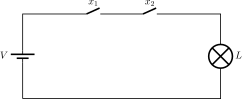
\includegraphics[width=199.3pt]{lect_2_switching_circuit_and}\caption{AND}\label{fig:sw-and}
\end{subfigure}
\hfill
\begin{subfigure}[b]{201.3pt}\centering
  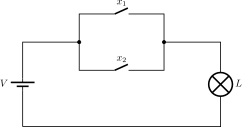
\includegraphics[width=199.3pt]{lect_2_switching_circuit_or}\caption{OR}\label{fig:sw-or}
\end{subfigure}
\\[6pt]
\begin{subfigure}[b]{158.8pt}\centering
  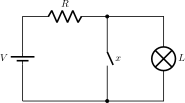
\includegraphics[width=156.8pt]{lect_2_switching_circuit_not}\caption{NOT}\label{fig:sw-not}
\end{subfigure}
\caption{Switching circuits for the three basic functions.}\label{fig:sw}
\end{figure}

\paragraph{NOT: a switch that diverts current.} Suppose the lamp should be on when the switch is \emph{open}. In \cref{fig:sw-not} current flows through the resistor $R$ and the lamp when switch $S$ is open ($x=0$); closing $S$ ($x=1$) short-circuits the lamp to ground. Hence $L = x'$.

\subsection{Truth tables}
A \term{truth table} lists the value of a function for every combination of its inputs; a function of $n$ variables has $2^n$ rows. The truth tables of the basic functions are in \cref{tab:basic-tt}. A truth table is the most complete and unambiguous specification of a combinational function, and it is the usual starting point of a design.

\begin{table}[htbp]
\centering
\caption{Truth tables of AND, OR and NOT.}
\label{tab:basic-tt}
\begin{tabular}{cc|c}
\toprule
$x_1$&$x_2$&$x_1x_2$\\ \midrule
0&0&0\\0&1&0\\1&0&0\\1&1&1\\ \bottomrule
\end{tabular}\qquad\qquad
\begin{tabular}{cc|c}
\toprule
$x_1$&$x_2$&$x_1+x_2$\\ \midrule
0&0&0\\0&1&1\\1&0&1\\1&1&1\\ \bottomrule
\end{tabular}\qquad\qquad
\begin{tabular}{c|c}
\toprule
$x$&$x'$\\ \midrule
0&1\\1&0\\ \bottomrule
\end{tabular}
\end{table}

\section{Logic Gates and Networks}\label{sec:gates}
Each basic operation is implemented by an electronic circuit called a \term{logic gate}, drawn with the standard symbols of \cref{fig:gate-symbols}. A gate has one or more inputs and one output. Gates are connected into a \term{logic network} (or logic circuit) that implements a larger function. For example, \cref{fig:logic-network} shows the function $f=(x_1+x_2)\cdot x_3$ realised by an OR gate feeding an AND gate.

\begin{figure}[htbp]
\centering
\begin{subfigure}[b]{138.7pt}\centering
  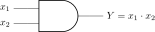
\includegraphics[width=136.7pt]{lect_2_and_symbol}\caption{AND}
\end{subfigure}
\hfill
\begin{subfigure}[b]{142.4pt}\centering
  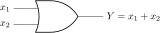
\includegraphics[width=140.4pt]{lect_2_or_symbol}\caption{OR}
\end{subfigure}
\hfill
\begin{subfigure}[b]{99.1pt}\centering
  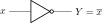
\includegraphics[width=97.1pt]{lect_2_not_symbol}\caption{NOT (inverter)}
\end{subfigure}
\caption{Graphical symbols of the basic gates.}\label{fig:gate-symbols}
\end{figure}

\figw{168.6pt}{lect_2_logic_network}{A logic network for $f=(x_1+x_2)\cdot x_3$: an OR gate feeding an AND gate.}{fig:logic-network}

\begin{lstlisting}[caption={VHDL description of $f=(x_1+x_2)\cdot x_3$.},label={lst:logic-function}]
library IEEE;
use IEEE.STD_LOGIC_1164.ALL;

entity logic_function is
  port (x1, x2, x3 : in  std_logic;
        f          : out std_logic);
end logic_function;

architecture behavioral of logic_function is
begin
  f <= (x1 or x2) and x3;
end behavioral;
\end{lstlisting}

\subsection{A first look at VHDL}
A hardware description language lets us write a circuit as text. A VHDL design unit has two parts, illustrated by \cref{lst:logic-function}.
\begin{itemize}
  \item The \code{entity} declares the \emph{interface}: the name of the circuit and its \code{port}s, each with a direction (\code{in} or \code{out}) and a type. We use \code{std_logic}, a one-bit type from the library \code{IEEE.std_logic_1164}.
  \item The \code{architecture} describes the \emph{behaviour} or structure. The statement \code{f <= (x1 or x2) and x3;} is a \term{concurrent signal assignment}: it describes a gate network that evaluates continuously, not a step executed once. Operators \code{and}, \code{or}, \code{not}, \code{xor}, \dots{} correspond directly to gates.
\end{itemize}
Appendix~\ref{app:vhdl} summarises the language elements used in this book.

\section{Logic Synthesis}\label{sec:synthesis}
\termx{Logic synthesis}{logic synthesis} is the process of producing a logic circuit that implements a desired function, usually given as a truth table or a Boolean expression. The primary goal is correctness; the secondary goal is optimisation: a circuit that is smaller, faster or uses less power. A function can be synthesised by looking at the rows where it is 1 or at the rows where it is 0, which leads to two standard forms.

\subsection{Sum of products and minterms}
A \term{minterm} of $n$ variables is a product (AND) term in which every variable appears exactly once, either complemented or not. Each minterm is 1 for exactly one row of the truth table, and the row number $i$ (read as a binary number) names the minterm $m_i$: a variable is complemented if its value in that row is 0 and uncomplemented if it is 1.

\begin{keypoint}[Synthesis of a sum of products]
(1)~Mark the rows in which $f=1$. (2)~Write the minterm of each marked row. (3)~OR the minterms together. The result is the \term{canonical sum of products} (canonical SOP), abbreviated $f=\Sm(\dots)$.
\end{keypoint}

\subsection{Product of sums and maxterms}
Dually, a \term{maxterm} is a sum (OR) term containing every variable once; it is 0 for exactly one row, and the maxterm $M_i$ is formed with a variable uncomplemented if its value in the row is 0 and complemented if it is 1. The \term{canonical product of sums} (canonical POS) ANDs the maxterms of all rows in which $f=0$: $f=\PM(\dots)$. Note that $m_i' = M_i$.

\begin{example}{SOP and POS of one function}{sop-pos}
The function $f(a,b,c)$ is 1 whenever $c=1$ (\cref{tab:sop-pos}).

\textbf{SOP:} the rows with $f=1$ are 1, 3, 5, 7, hence
\[
 f = a'b'c + a'bc + ab'c + abc = m_1+m_3+m_5+m_7 = \Sm(1,3,5,7).
\]
\textbf{POS:} the rows with $f=0$ are 0, 2, 4, 6, hence
\[
 f = (a+b+c)(a+b'+c)(a'+b+c)(a'+b'+c) = M_0M_2M_4M_6 = \PM(0,2,4,6).
\]
Both are correct and equal; in this case each simplifies to $f=c$.
\end{example}

\begin{table}[htbp]
\centering
\caption{Truth table of \cref{ex:sop-pos} with minterms and maxterms.}
\label{tab:sop-pos}
\begin{tabular}{ccc|c|ll}
\toprule
$a$&$b$&$c$&$f$&Minterm&Maxterm\\ \midrule
0&0&0&0&$m_0 = a'b'c'$&$\mathbf{M_0 = a+b+c}$\\
0&0&1&1&$\mathbf{m_1 = a'b'c}$&$M_1 = a+b+c'$\\
0&1&0&0&$m_2 = a'bc'$&$\mathbf{M_2 = a+b'+c}$\\
0&1&1&1&$\mathbf{m_3 = a'bc}$&$M_3 = a+b'+c'$\\
1&0&0&0&$m_4 = ab'c'$&$\mathbf{M_4 = a'+b+c}$\\
1&0&1&1&$\mathbf{m_5 = ab'c}$&$M_5 = a'+b+c'$\\
1&1&0&0&$m_6 = abc'$&$\mathbf{M_6 = a'+b'+c}$\\
1&1&1&1&$\mathbf{m_7 = abc}$&$M_7 = a'+b'+c'$\\
\bottomrule
\end{tabular}
\end{table}

\subsection{Minimality and simplification}
A canonical expression is seldom the cheapest. The cost of a circuit is roughly the number of gates and gate inputs, so we try to find an equivalent expression with fewer literals.

\begin{example}{Algebraic simplification}{simplify}
Simplify the canonical SOP $f(x_1,x_2) = x_1'x_2' + x_1'x_2 + x_1x_2$, whose truth table is 1, 1, 0, 1 for $x_1x_2 = 00, 01, 10, 11$.

\textbf{Solution.}
\begin{align*}
f &= x_1'(x_2'+x_2) + x_1x_2 && \text{(distributive)}\\
  &= x_1'\cdot 1 + x_1x_2 = x_1' + x_1x_2 && (x+x'=1)\\
  &= (x_1'+x_1)(x_1'+x_2) && \text{(distributive, OR form)}\\
  &= 1\cdot(x_1'+x_2) = x_1' + x_2 .
\end{align*}
The canonical form needs three 2-input AND gates, two inverters and a 3-input OR; the simplified form needs one inverter and one 2-input OR (\cref{fig:orig-simpl}).
\end{example}

\begin{figure}[htbp]
\centering
\begin{subfigure}[b]{215.4pt}\centering
  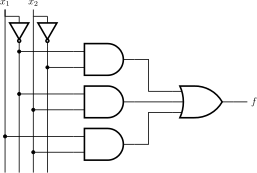
\includegraphics[width=213.4pt]{lect_2_sop_circuit}\caption{canonical form}
\end{subfigure}
\hfill
\begin{subfigure}[b]{147.2pt}\centering
  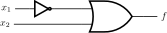
\includegraphics[width=145.2pt]{lect_2_simplified_circuit}\caption{simplified form $x_1'+x_2$}
\end{subfigure}
\caption{Two circuits for the same function of \cref{ex:simplify}.}\label{fig:orig-simpl}
\end{figure}

\Cref{lst:two-arch} shows an advantage of VHDL: one entity can have several architectures, so the unsimplified and simplified descriptions can be kept side by side and checked against each other in simulation. A particular architecture is selected by \emph{direct entity instantiation}, \code{UUT : entity work.Logic_Function(RTL_Simplified) port map (\dots);}, or by a \code{configuration} declaration.

\begin{lstlisting}[caption={One entity with two architectures: canonical and simplified.},label={lst:two-arch}]
library ieee;
use ieee.std_logic_1164.all;

entity Logic_Function is
  port (x1, x2 : in  std_logic;
        f      : out std_logic);
end entity Logic_Function;

-- canonical sum of products:  f = x1'x2' + x1'x2 + x1x2
architecture RTL_Canonical of Logic_Function is
begin
  f <= (not x1 and not x2) or (not x1 and x2) or (x1 and x2);
end architecture RTL_Canonical;

-- simplified:  f = x1' + x2
architecture RTL_Simplified of Logic_Function is
begin
  f <= not x1 or x2;
end architecture RTL_Simplified;
\end{lstlisting}

\section{Design Examples}\label{sec:examples2}
A systematic design proceeds from a word description to a truth table, to a Boolean expression, to a simplified expression and finally to a circuit and its VHDL description. We illustrate the flow with four examples.

\subsection{Three-way light control}
\begin{example}{Light controlled from three doors}{three-way}
A room has three doors, each with a switch $x_1,x_2,x_3$, that control a single light. Flipping any switch must toggle the light. When all switches are open (0) the light is off. Design the circuit.

\textbf{Truth table.} If one switch is closed the light is on; if two are closed it is off (flipping one switch from the one-closed state switched it off); if all three are closed it is on again. So $f=1$ in rows 1, 2, 4 and 7 (\cref{tab:threeway}).

\textbf{Expression.} The canonical SOP is
\[
 f = x_1'x_2'x_3 + x_1'x_2x_3' + x_1x_2'x_3' + x_1x_2x_3 .
\]
This is already the simplest SOP, but it has a compact form: $f$ is 1 when an \emph{odd} number of inputs is 1, which is the \term{exclusive OR} (XOR) of the three variables, $f = x_1\xor x_2\xor x_3$, where $x\xor y = x'y+xy'$.
\end{example}

\begin{table}[htbp]
\centering
\caption{Truth table for the three-way light.}
\label{tab:threeway}
\begin{tabular}{ccc|c}
\toprule
$x_1$&$x_2$&$x_3$&$f$\\ \midrule
0&0&0&0\\0&0&1&\textbf{1}\\0&1&0&\textbf{1}\\0&1&1&0\\
1&0&0&\textbf{1}\\1&0&1&0\\1&1&0&0\\1&1&1&\textbf{1}\\ \bottomrule
\end{tabular}
\end{table}

\Cref{lst:threeway} gives both descriptions and a testbench. The testbench is explained in \cref{sec:testbench}.

\begin{lstlisting}[caption={Three-way light: two architectures.},label={lst:threeway}]
library ieee;
use ieee.std_logic_1164.all;

entity three_way_light is
  port (x1, x2, x3 : in  std_logic;
        f          : out std_logic);
end three_way_light;

-- direct sum of products
architecture arch_sop of three_way_light is
begin
  f <= (not x1 and not x2 and x3) or (not x1 and x2 and not x3) or
       (x1 and not x2 and not x3) or (x1 and x2 and x3);
end arch_sop;

-- XOR form: same function, simpler description
architecture arch_simplified of three_way_light is
begin
  f <= x1 xor x2 xor x3;
end arch_simplified;
\end{lstlisting}

\subsection{Two-to-one multiplexer}
\begin{example}{Multiplexer}{mux}
Design a circuit that selects between two data inputs $x_1$ and $x_2$ using a control input $s$: $f=x_1$ if $s=0$ and $f=x_2$ if $s=1$.

\textbf{Truth table.} Rows are ordered $s\,x_1x_2$ (\cref{tab:mux}). $f=1$ in rows 2, 3, 5 and 7.

\textbf{Expression and simplification.}
\begin{align*}
f &= s'x_1x_2' + s'x_1x_2 + sx_1'x_2 + sx_1x_2\\
  &= s'x_1(x_2'+x_2) + sx_2(x_1'+x_1) = s'x_1 + sx_2 .
\end{align*}
The circuit is two AND gates, one inverter and one OR gate (\cref{fig:mux}).
\end{example}

\begin{table}[htbp]
\centering
\caption{Truth table of a 2-to-1 multiplexer.}
\label{tab:mux}
\begin{tabular}{ccc|c}
\toprule
$s$&$x_1$&$x_2$&$f$\\ \midrule
0&0&0&0\\0&0&1&0\\0&1&0&\textbf{1}\\0&1&1&\textbf{1}\\
1&0&0&0\\1&0&1&\textbf{1}\\1&1&0&0\\1&1&1&\textbf{1}\\ \bottomrule
\end{tabular}
\end{table}

\begin{figure}[htbp]
\centering
\begin{subfigure}[b]{223.9pt}\centering
  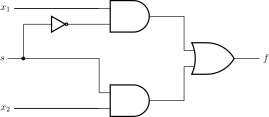
\includegraphics[width=221.9pt]{lect_2_mux_2to1}\caption{circuit for $f=s'x_1+sx_2$}
\end{subfigure}
\hfill
\begin{subfigure}[b]{75.3pt}\centering
  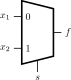
\includegraphics[width=73.3pt]{lect_2_mux_2_to_1_symbol}\caption{graphical symbol}
\end{subfigure}
\caption{A 2-to-1 multiplexer. The multiplexer is one of the most useful blocks in digital design and is studied further in \cref{ch:blocks}.}\label{fig:mux}
\end{figure}

\subsection{Car safety alarm}
\begin{example}{Car alarm}{car-alarm}
A car alarm $A$ must sound if (1)~the key is in the ignition ($K=1$) and the door is not closed ($D=0$), or (2)~the door is closed ($D=1$), the key is in ($K=1$), the driver is in the seat ($S=1$) and the seat belt is not fastened ($B=0$). Derive a minimal expression.

\textbf{Solution.} Translating the conditions, $A = KD' + DKSB'$. Factor out $K$: $A = K(D' + DSB')$. Using the identity $X + X'Y = X+Y$ (proved by distributing: $X+X'Y=(X+X')(X+Y)=X+Y$) with $X=D'$,
\[
  A = K\,(D' + SB').
\]
This needs one inverter for $D$, one for $B$, one AND, one OR and one more AND (\cref{fig:car-alarm}), far fewer than the original expression, and the VHDL is a single line, \cref{lst:car-alarm}.
\end{example}

\begin{figure}[htbp]
\centering
\begin{subfigure}[b]{130.2pt}\centering
  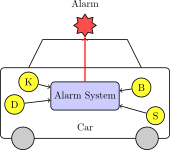
\includegraphics[width=128.2pt]{lect_2_car_alarm_sketch}\caption{the system}
\end{subfigure}
\hfill
\begin{subfigure}[b]{239.3pt}\centering
  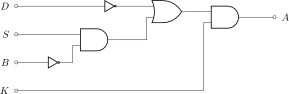
\includegraphics[width=237.3pt]{lect_2_car_alarm}\caption{circuit for $A=K(D'+SB')$}
\end{subfigure}
\caption{The car safety alarm of \cref{ex:car-alarm}.}\label{fig:car-alarm}
\end{figure}

\begin{lstlisting}[caption={Car alarm logic.},label={lst:car-alarm}]
library ieee;
use ieee.std_logic_1164.all;

entity car_alarm_logic is
  port (K, D, S, B : in  std_logic;
        A          : out std_logic);
end entity car_alarm_logic;

architecture rtl of car_alarm_logic is
begin
  A <= K and (not D or (S and not B));     -- A = K (D' + S B')
end architecture rtl;
\end{lstlisting}

\subsection{Half adder}
\begin{example}{Half adder}{half-adder}
Design a circuit that adds two bits $x$ and $y$ and produces a \emph{sum} bit $s$ and a \emph{carry} bit $c$.

\textbf{Truth table.} The arithmetic $0{+}0=00$, $0{+}1=01$, $1{+}0=01$, $1{+}1=10$ gives \cref{tab:ha}. The sum is 1 only when the inputs differ, so $s = x'y+xy' = x\xor y$; the carry is 1 only when both inputs are 1, so $c = xy$.
\end{example}

\begin{table}[htbp]
\centering
\caption{Half adder.}
\label{tab:ha}
\begin{tabular}{cc|cc}
\toprule
$x$&$y$&sum $s$&carry $c$\\ \midrule
0&0&0&0\\0&1&1&0\\1&0&1&0\\1&1&0&1\\ \bottomrule
\end{tabular}
\end{table}

The circuit is an XOR gate and an AND gate (\cref{fig:ha}). The half adder is the starting point of the arithmetic circuits of \cref{ch:arith}.

\begin{figure}[htbp]
\centering
\begin{subfigure}[b]{179.5pt}\centering
  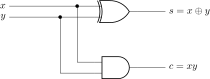
\includegraphics[width=177.5pt]{lect_2_half_adder}\caption{gate-level circuit}
\end{subfigure}
\hfill
\begin{subfigure}[b]{183.3pt}\centering
  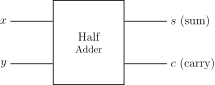
\includegraphics[width=181.3pt]{lect_2_half_adder_block}\caption{block diagram}
\end{subfigure}
\caption{Half adder.}\label{fig:ha}
\end{figure}

\begin{lstlisting}[caption={Half adder in VHDL (dataflow style).},label={lst:half-adder}]
library ieee;
use ieee.std_logic_1164.all;

entity half_adder is
  port (x, y : in  std_logic;     -- the two bits to add
        s, c : out std_logic);    -- sum and carry-out
end entity half_adder;

architecture dataflow of half_adder is
begin
  s <= x xor y;                   -- sum
  c <= x and y;                   -- carry
end architecture dataflow;
\end{lstlisting}

\section{The VHDL Testbench}\label{sec:testbench}
A \term{testbench} is a VHDL entity used to simulate and check another entity, the \emph{unit under test} (UUT). A testbench has no ports because it is closed: it generates its own stimulus and observes the UUT's response (\cref{fig:tb}). Writing a testbench takes four steps.
\begin{enumerate}
  \item \textbf{Instantiate} the UUT as a \code{component} (or by direct entity instantiation) and connect its ports to local signals.
  \item \textbf{Generate stimulus.} A \code{process} assigns values to the input signals and uses \code{wait for} statements to advance simulated time.
  \item \textbf{Observe} the outputs in the simulator's waveform window.
  \item \textbf{Verify.} Compare the waveform with the truth table, either by inspection or automatically with \code{assert} statements that report an error if an output is wrong.
\end{enumerate}

\figw{265.8pt}{lect_2_test_bench}{The relationship between a testbench and the unit under test (UUT).}{fig:tb}

\begin{lstlisting}[caption={A testbench for the three-way light that applies all eight input combinations.},label={lst:tb}]
library ieee;
use ieee.std_logic_1164.all;

entity three_way_light_tb is end entity;          -- no ports

architecture behavior of three_way_light_tb is
  signal x1, x2, x3 : std_logic := '0';            -- inputs to the UUT
  signal f          : std_logic;                   -- output of the UUT
begin
  uut : entity work.three_way_light(arch_simplified)
        port map (x1 => x1, x2 => x2, x3 => x3, f => f);

  stim_proc : process
  begin
    wait for 100 ns;                               -- let the simulator settle
    x1<='0'; x2<='0'; x3<='0'; wait for 10 ns;     -- expect f = 0
    x1<='0'; x2<='0'; x3<='1'; wait for 10 ns;     -- expect f = 1
    x1<='0'; x2<='1'; x3<='0'; wait for 10 ns;     -- expect f = 1
    x1<='0'; x2<='1'; x3<='1'; wait for 10 ns;     -- expect f = 0
    x1<='1'; x2<='0'; x3<='0'; wait for 10 ns;     -- expect f = 1
    x1<='1'; x2<='0'; x3<='1'; wait for 10 ns;     -- expect f = 0
    x1<='1'; x2<='1'; x3<='0'; wait for 10 ns;     -- expect f = 0
    x1<='1'; x2<='1'; x3<='1'; wait for 10 ns;     -- expect f = 1
    wait;                                          -- stop the process
  end process;
end architecture behavior;
\end{lstlisting}

\Cref{fig:sim-threeway} shows the waveform obtained by simulating \cref{lst:tb} in the Intel\textregistered\ Questa simulator. Each of the eight 10~ns intervals corresponds to one row of \cref{tab:threeway}; the output $f$ is high in rows 1, 2, 4 and 7, as predicted.

\begin{figure}[htbp]
\centering
\wavesplit{lect_2_three_way_light_sim}{4}
\caption{Simulation of the three-way light in Intel Questa (author's screenshot).}\label{fig:sim-threeway}
\end{figure}

\begin{caution}
Writing the expected value of $f$ only by looking at the simulation output proves nothing: the simulator will always give you the answer your design computes. Work out the expected outputs from the truth table \emph{first}, then compare.
\end{caution}

\begin{chaptersummary}
\begin{itemize}
  \item \textbf{Boolean algebra} has two values and three operations (AND, OR, NOT). Its theorems appear in dual pairs; \textbf{De Morgan's theorem} gives the complement of a sum or a product.
  \item An identity can be proved by \textbf{perfect induction}: check every row of the truth table.
  \item A \textbf{truth table} fully specifies a combinational function. \textbf{Gates} implement the basic operations and are connected into \textbf{logic networks}.
  \item A function with $f=1$ in rows $i_1,i_2,\dots$ has the canonical \textbf{SOP} $\Sm(i_1,i_2,\dots)$; with $f=0$ in rows $j_1,\dots$ it has the canonical \textbf{POS} $\PM(j_1,\dots)$.
  \item \textbf{Simplification} reduces the number of gates and inputs; the same function may have many equivalent expressions.
  \item The design flow is: \emph{word problem $\to$ truth table $\to$ expression $\to$ simplification $\to$ circuit $\to$ VHDL $\to$ testbench}.
  \item A VHDL \textbf{entity} defines the interface and an \textbf{architecture} the behaviour; a \textbf{testbench} stimulates the unit under test and lets us check it against the truth table.
\end{itemize}
\end{chaptersummary}

\chapsec{Exercises}
\begin{exlist}
  \item \textbf{Majority function.} A majority function is true when more than half of its inputs are true. (a)~Write the truth table of a 3-input majority function $f(x,y,z)$. (b)~Write its canonical SOP. (c)~Simplify it algebraically. (d)~Draw the circuit using AND, OR and NOT gates. (e)~Write VHDL and a testbench that applies all eight input combinations, and show the waveform.
  \item \textbf{Home alarm.} The alarm $A$ sounds if the system is armed ($S=1$) \emph{and} either the front door ($D=1$) or the window ($W=1$) is open. It never sounds if the system is not armed. Give the truth table, the Boolean expression, the circuit, and a simulation of the case $S=1$, $D=1$.
  \item \textbf{Line-following robot.} A robot has three sensors $L$, $C$, $R$ (value 0 over the black line, 1 over the white surface) and two motors $M_L$, $M_R$. It must \emph{go forward} ($M_L=M_R=1$) when centred ($L=1,C=0,R=1$); \emph{turn right} ($M_L=1, M_R=0$) when it drifts left ($L=1,C=1,R=0$); \emph{turn left} ($M_L=0,M_R=1$) when it drifts right ($L=0,C=1,R=1$); and \emph{stop} ($M_L=M_R=0$) in every other case. (a)~Write the truth table. (b)~Write SOP expressions for $M_L$ and $M_R$ and simplify them. (c)~Draw the circuits. (d)~Simulate all four behaviours.
  \item \textbf{Seven-segment decoder.} A seven-segment display has segments $a,b,c,d,e,f,g$ (\cref{fig:sevenseg}). Design a decoder with a 4-bit BCD input $b_3b_2b_1b_0$ that lights the segments to show the digits 0--9. Assume a \emph{common anode} display, in which a segment lights when its control signal is \emph{low}. (a)~Give the truth table, treating the input values 10--15 as don't-cares. (b)~Find the simplified SOP for segment $a$ (you may postpone the other segments until you have learnt Karnaugh maps in \cref{ch:kmap}). (c)~Draw the circuit for segment $a$.
  \item Use truth tables to prove: (a)~$x+xy=x$; (b)~$x+yz=(x+y)(x+z)$; (c)~$xy+x'z+yz=xy+x'z$.
  \item Write the dual of each identity: (a)~$x+x'y=x+y$; (b)~$(x+y)(x+z)=x+yz$; (c)~$xy+x'z+yz = xy+x'z$.
  \item Use De Morgan's theorem to find the complement of each function and express it as a sum of products: (a)~$F=x+yz'$; (b)~$F=x'y+xy'$; (c)~$F=(a+b)(c+d)$.
  \item Simplify algebraically, stating the identity used in each step: (a)~$F=x'y+xy+x'y'$; (b)~$F=(x+y)(x+y')(x'+z)$; (c)~$F=xy+x'z+yz$.
  \item A function is defined by $f=\Sm(0,3,5,6)$ of three variables $x,y,z$. (a)~Write the canonical SOP and the canonical POS. (b)~Describe in words when $f=1$. (c)~Give the complement $f'$ in $\Sm$ notation.
  \item Design a circuit with inputs $x_1,x_2,x_3$ whose output is 1 if and only if \emph{exactly two} of the inputs are 1. Give the canonical SOP and draw the circuit.
  \item Design a circuit with two 2-bit inputs $A=A_1A_0$ and $B=B_1B_0$ whose output $E$ is 1 when $A=B$. \emph{Hint:} $A=B$ if and only if each pair of corresponding bits is equal, and two bits are equal when their XOR is 0.
  \item How many different Boolean functions exist of (a)~two variables; (b)~three variables; (c)~$n$ variables? \emph{Hint:} each function is defined by a column of the truth table.
  \item The three-way light of \cref{ex:three-way} is extended to a corridor with four switches $x_1,\dots,x_4$, each of which toggles the light. (a)~Write the function using XOR. (b)~How many minterms does the canonical SOP contain?
\end{exlist}

\begin{figure}[htbp]
\centering
\begin{tikzpicture}[x=1cm,y=1cm]
  \tikzset{seg/.style={fill=kmutnborange!85, draw=none}, lab/.style={font=\sffamily\scriptsize}}
  \fill[seg] (0.15,2.35) -- (0.35,2.55) -- (1.65,2.55) -- (1.85,2.35) -- (1.65,2.15) -- (0.35,2.15) -- cycle;
  \fill[seg] (0.1,1.1) -- (0.3,1.3) -- (0.3,2.1) -- (0.1,2.3) -- (-0.1,2.1) -- (-0.1,1.3) -- cycle;
  \fill[seg] (1.9,1.1) -- (2.1,1.3) -- (2.1,2.1) -- (1.9,2.3) -- (1.7,2.1) -- (1.7,1.3) -- cycle;
  \fill[seg] (0.15,1.05) -- (0.35,1.25) -- (1.65,1.25) -- (1.85,1.05) -- (1.65,0.85) -- (0.35,0.85) -- cycle;
  \fill[seg] (0.1,-0.1) -- (0.3,0.1) -- (0.3,0.8) -- (0.1,1.0) -- (-0.1,0.8) -- (-0.1,0.1) -- cycle;
  \fill[seg] (1.9,-0.1) -- (2.1,0.1) -- (2.1,0.8) -- (1.9,1.0) -- (1.7,0.8) -- (1.7,0.1) -- cycle;
  \fill[seg] (0.15,-0.15) -- (0.35,0.05) -- (1.65,0.05) -- (1.85,-0.15) -- (1.65,-0.35) -- (0.35,-0.35) -- cycle;
  \node[lab] at (1,2.85) {a}; \node[lab] at (2.45,1.7) {b}; \node[lab] at (2.45,0.45) {c};
  \node[lab] at (1,-0.7) {d}; \node[lab] at (-0.45,0.45) {e}; \node[lab] at (-0.45,1.7) {f}; \node[lab] at (1,1.45) {g};
\end{tikzpicture}
\caption{Segment labels of the seven-segment display used in Exercise~2.4.}
\label{fig:sevenseg}
\end{figure}

\chapsec{Further Reading}
The reader who wants a systematic treatment of Boolean algebra and switching functions will find it in Brown and Vranesic~\cite{brown2009} and in Mano and Ciletti~\cite{mano2018}; Wakerly~\cite{wakerly2006} gives a particularly careful account of the relation between gates, expressions and timing. Shannon's thesis~\cite{shannon1938} remains very readable. For VHDL, see Ashenden~\cite{ashenden2008} and the language standard~\cite{ieee1076}.

\chapter{Logic Optimisation with Karnaugh Maps}\label{ch:kmap}

\begin{objectives}
After studying this chapter you will be able to:
\begin{itemize}
  \item draw two-, three- and four-variable Karnaugh maps and plot a function on them;
  \item find all prime implicants, identify the essential ones, and derive a minimal sum-of-products (SOP) expression;
  \item exploit don't-care conditions to obtain simpler circuits;
  \item derive a minimal product-of-sums (POS) expression by grouping the 0s;
  \item implement SOP and POS expressions with two-level NAND--NAND and NOR--NOR circuits, and explain why NAND and NOR are universal gates;
  \item use XOR and XNOR gates, recognise odd and even functions, and design parity generators and checkers.
\end{itemize}
\end{objectives}

\section{The Need for Optimisation}
In the design flow of \cref{fig:comb-flow}, the step after deriving a Boolean expression from a truth table (for example with minterms, \cref{sec:synthesis}) is \emph{optimisation}. A simpler expression gives a circuit with fewer gates, which is cheaper, usually faster and consumes less power. Algebraic manipulation, as in \cref{ex:simplify}, can do the job, but it follows no fixed rule: it is not obvious which identity to apply next, nor when to stop. The \term{Karnaugh map} turns simplification into a pattern-recognition task that a person can perform reliably for up to about five variables.

\figside{540.1pt}{lect_3_combinational_design_flow}{Design flow of a combinational circuit: specification, truth table, Boolean expression, optimisation and implementation.}{fig:comb-flow}

\section{The Karnaugh Map}
The Karnaugh map (K-map), introduced by Maurice Karnaugh in 1953~\cite{karnaugh1953}, is a pictorial form of the truth table. It is a diagram made up of squares, \emph{each square representing one minterm}. It is arranged so that squares that are \emph{adjacent}, horizontally or vertically, represent minterms that differ in exactly one variable. Two such minterms can be combined by the combining identity $xy+xy'=x$, which removes the variable that changes. The map thus displays, at a glance, all the pairs of minterms that can be merged.

\figw{180.0pt}{lect_3_kmap_example}{A Karnaugh map is a truth table rearranged so that neighbouring squares differ in one variable.}{fig:kmap-example}

\subsection{The two-variable map}
A function of two variables has $2^2=4$ minterms, so its map has four squares (\cref{fig:kmap2}). The rows correspond to the values of $x$ and the columns to the values of $y$. To plot a function, write a 1 in the square of every minterm of the function. For instance $f=xy$ is the single minterm $m_3$, while $f=x+y=m_1+m_2+m_3$ has three 1s.

\begin{figure}[htbp]
\centering
\begin{subfigure}[b]{128.7pt}\centering
  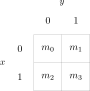
\includegraphics[width=126.7pt]{lect_3_kmap_2var_minterm}\caption{minterms}
\end{subfigure}
\hfill
\begin{subfigure}[b]{128.7pt}\centering
  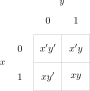
\includegraphics[width=126.7pt]{lect_3_kmap_2var_variable}\caption{variables}
\end{subfigure}
\hfill
\begin{subfigure}[b]{128.7pt}\centering
  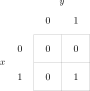
\includegraphics[width=126.7pt]{lect_3_kmap_x_and_y}\caption{$f=xy$}
\end{subfigure}
\\[6pt]
\begin{subfigure}[b]{128.7pt}\centering
  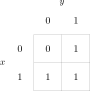
\includegraphics[width=126.7pt]{lect_3_kmap_x_or_y}\caption{$f=x+y$}
\end{subfigure}
\caption{Two-variable K-maps: the layout of minterms and variables, and two plotted functions.}\label{fig:kmap2}
\end{figure}

\subsection{The three-variable map}
Three variables give $2^3 = 8$ squares, arranged in two rows and four columns (\cref{fig:kmap3}). The key point is that the columns are ordered in \term{Gray code}, $00, 01, 11, 10$, not in binary order: in a Gray code only one bit changes between consecutive code words. Because of this, horizontally adjacent squares differ in exactly one variable. The ordering also makes the \emph{leftmost and rightmost columns adjacent}, as if the map were wrapped around a cylinder (column $10$ is adjacent to column $00$).

Two adjacent 1s can be merged to remove one variable. For example $m_5$ and $m_7$ are adjacent: $xy'z + xyz = xz(y'+y) = xz$.

\figw{180.0pt}{lect_3_kmap_3var_structure}{Structure of the three-variable K-map. Columns follow a Gray code and wrap around.}{fig:kmap3}

\subsection{Rules for simplification}
\begin{keypoint}[Rules for grouping on a K-map]
The aim is to cover all the 1s of the map with as few and as large groups as possible.
\begin{enumerate}
  \item Groups must be \textbf{rectangles} containing $1, 2, 4, 8,\dots$ squares (a power of two).
  \item Make each group \textbf{as large as possible}; a group of four is better than two groups of two.
  \item \textbf{Every 1 must be covered} by at least one group.
  \item Groups \textbf{may overlap} if this allows larger groups.
  \item \textbf{Wrap-around} adjacency is allowed: the left and right edges, and the top and bottom edges, are neighbours.
  \item Use the \textbf{fewest groups} that cover all the 1s.
\end{enumerate}
Each group gives one product term; the variables that take a constant value over the whole group appear in the term (uncomplemented if the constant is 1, complemented if it is 0) and the variables that change are eliminated. The simplified function is the OR of the product terms. A group of $2^k$ squares eliminates $k$ variables.
\end{keypoint}

\begin{example}{Two groups of two}{kmap1}
Simplify $F(x,y,z)=\Sm(2,3,4,5)$.

\textbf{Solution.} Plot 1s in squares 2, 3, 4 and 5 (\cref{fig:ex31}). Minterms $m_2,m_3$ ($x'yz'$ and $x'yz$) are adjacent and combine to $x'y$; $m_4,m_5$ ($xy'z'$ and $xy'z$) combine to $xy'$. Hence
\[ F = x'y + xy' = x\xor y. \]
\end{example}

\begin{example}{Groups with wrap-around}{kmap2}
Simplify $F(x,y,z)=\Sm(3,4,6,7)$.

\textbf{Solution.} $m_3$ and $m_7$ ($x'yz$, $xyz$) combine to $yz$. $m_4$ and $m_6$ ($xy'z'$, $xyz'$) are adjacent \emph{through the wrap-around} (column $00$ to column $10$) and combine to $xz'$. Hence $F = yz + xz'$ (\cref{fig:ex32}).
\end{example}

\begin{example}{A group of four}{kmap3}
Simplify $F(x,y,z)=\Sm(0,2,4,6)$.

\textbf{Solution.} All four 1s form a single group (the two outer columns, joined by wrap-around). Over this group $x$ takes both values and so does $y$, so both are eliminated; $z$ is 0 in all four squares, so $z'$ remains: $F = z'$ (\cref{fig:ex33}). A group of four eliminates two variables.
\end{example}

\begin{example}{Overlapping groups}{kmap4}
Simplify $F(x,y,z)=\Sm(0,2,4,5,6)$.

\textbf{Solution.} The largest group covers $m_0,m_2,m_4,m_6$ and gives $z'$. The 1 in $m_5$ is not yet covered; the largest group containing it is $m_4,m_5$, which gives $xy'$. Note that $m_4$ belongs to both groups, which is allowed and gives the simplest result: $F = z' + xy'$ (\cref{fig:ex34}).
\end{example}

\begin{figure}[htbp]
\centering
\begin{subfigure}[b]{182.0pt}\centering
  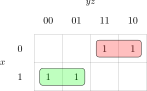
\includegraphics[width=180.0pt]{kmap_3var_ex1}\caption{\cref{ex:kmap1}}\label{fig:ex31}
\end{subfigure}
\hfill
\begin{subfigure}[b]{182.0pt}\centering
  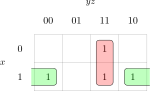
\includegraphics[width=180.0pt]{lect_3_kmap_3var_ex2}\caption{\cref{ex:kmap2}}\label{fig:ex32}
\end{subfigure}
\\[6pt]
\begin{subfigure}[b]{182.0pt}\centering
  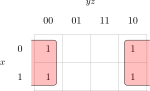
\includegraphics[width=180.0pt]{lect_3_kmap_3var_ex3}\caption{\cref{ex:kmap3}}\label{fig:ex33}
\end{subfigure}
\hfill
\begin{subfigure}[b]{182.0pt}\centering
  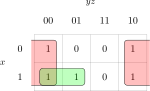
\includegraphics[width=180.0pt]{kmap_3var_ex4}\caption{\cref{ex:kmap4}}\label{fig:ex34}
\end{subfigure}
\caption{K-maps for \cref{ex:kmap1,ex:kmap2,ex:kmap3,ex:kmap4}.}\label{fig:ex3x}
\end{figure}

\section{Prime Implicants}
The grouping procedure can be stated more precisely with three definitions.

\begin{definition}{Implicants}{implicant}
An \term{implicant} of a function is a product term that covers one or more minterms of the function (every group of 1s on the map is an implicant). A \term{prime implicant} (PI) is an implicant that cannot be combined with another to form a larger implicant, that is, a group of 1s that is as large as it can be. An \term{essential prime implicant} (EPI) is a prime implicant that covers at least one minterm covered by no other prime implicant.
\end{definition}

\begin{keypoint}[Minimisation procedure]
\begin{enumerate}
  \item Find all prime implicants.
  \item Include all essential prime implicants.
  \item Choose the smallest set of the remaining prime implicants that covers all the 1s not yet covered.
\end{enumerate}
\end{keypoint}

\section{The Four-Variable Map}
A function of four variables has 16 minterms and a $4\times4$ map (\cref{fig:kmap4}). Both the rows (variables $w,x$) and the columns (variables $y,z$) are in Gray-code order $00,01,11,10$. Wrap-around applies in both directions: the top row is adjacent to the bottom row, and the left column to the right column; in effect the map is a torus. The four corners are therefore adjacent to one another.

\figw{186.2pt}{lect_3_kmap_4x4_structure}{Structure of the four-variable K-map.}{fig:kmap4}

\begin{example}{Four-variable simplification}{kmap5}
Simplify $F(w,x,y,z)=\Sm(0,1,2,4,5,6,8,9,12,13,14)$.

\textbf{Solution.} The map is \cref{fig:ex35}. Look for the largest groups first.
\begin{itemize}
  \item The eight squares in the two columns where $y=0$ (minterms 0, 1, 4, 5, 8, 9, 12, 13) form a group of eight: the term is $y'$.
  \item $m_0,m_2,m_4,m_6$ form a group of four (using the wrap-around between columns $00$ and $10$): $w'z'$.
  \item $m_4,m_6,m_{12},m_{14}$ form a group of four (again by wrap-around): $xz'$.
\end{itemize}
All eleven 1s are covered, and each group is needed ($y'$ is the only group containing $m_1,m_9$; $w'z'$ is the only one containing $m_2$; $xz'$ is the only one containing $m_{14}$). Hence
\[ F = y' + w'z' + xz'. \]
\end{example}

\begin{example}{More than one minimal expression}{kmap6}
Simplify $F(A,B,C,D)=\Sm(0,1,2,5,7,8,9,10,13,15)$.

\textbf{Solution.} The prime implicants are $B'C'$ ($m_0,m_1,m_8,m_9$), $B'D'$ ($m_0,m_2,m_8,m_{10}$), $BD$ ($m_5,m_7,m_{13},m_{15}$) and $C'D$ ($m_1,m_5,m_9,m_{13}$). $B'D'$ is essential because it alone covers $m_2$ and $m_{10}$, and $BD$ is essential because it alone covers $m_7$ and $m_{15}$. The essential prime implicants cover all the 1s except $m_1$ and $m_9$, and either of the remaining prime implicants covers both. There are therefore \emph{two} minimal expressions (\cref{fig:ex36}):
\[ F = BD + B'D' + B'C' \qquad\text{or}\qquad F = BD + B'D' + C'D. \]
They have the same cost; the choice may depend on which signals are already available.
\end{example}

\begin{figure}[htbp]
\centering
\begin{subfigure}[b]{188.2pt}\centering
  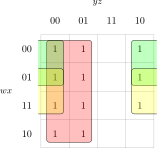
\includegraphics[width=186.2pt]{lect_3_kmap_4x4_ex5}\caption{\cref{ex:kmap5}}\label{fig:ex35}
\end{subfigure}
\hfill
\begin{subfigure}[b]{190.2pt}\centering
  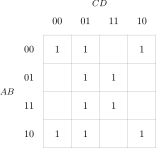
\includegraphics[width=188.2pt]{lect_3_kmap_4x4_ex6_1}\caption{plotted $F$}
\end{subfigure}
\\[6pt]
\begin{subfigure}[b]{190.2pt}\centering
  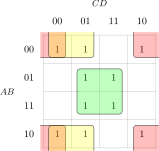
\includegraphics[width=188.2pt]{lect_3_kmap_4x4_ex6_sol_1}\caption{solution 1}
\end{subfigure}
\hfill
\begin{subfigure}[b]{190.2pt}\centering
  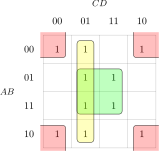
\includegraphics[width=188.2pt]{lect_3_kmap_4x4_ex6_sol_2}\caption{solution 2}
\end{subfigure}
\caption{(a)~\Cref{ex:kmap5}. (b--d)~\Cref{ex:kmap6}: the map and its two minimal covers.}\label{fig:ex36}
\end{figure}

\section{Don't-Care Conditions}\label{sec:dontcare}
In many designs the output for some input combinations is not specified. These are \term{don't-care conditions}. They arise because (a)~the input combination can never occur (for example, the six invalid codes $1010$ to $1111$ of a 4-bit BCD input), or (b)~the output for that input does not matter. On the map a don't-care is marked with an \textbf{X} (sometimes ``d''). The rules are:
\begin{itemize}
  \item treat an X as a 1 if this lets you form a larger group;
  \item otherwise treat it as a 0 (ignore it);
  \item you need \emph{not} cover all the X squares.
\end{itemize}

\begin{example}{Using don't-cares}{dontcare}
Simplify $F(w,x,y,z) = \Sm(1,3,7,11,15) + d(0,2,5)$.

\textbf{Solution.} See \cref{fig:dontcare}. The group $m_3,m_7,m_{11},m_{15}$ gives $yz$. The remaining 1, $m_1$, can be grouped with the don't-cares in two ways: $m_1,m_3,m_5,m_7$ gives $w'z$, and $m_0,m_1,m_2,m_3$ gives $w'x'$. Either is acceptable:
\[ F = yz + w'z \qquad\text{or}\qquad F = yz + w'x'. \]
Without don't-cares, $m_1$ could be combined only with $m_3$, giving a less simple term $w'x'z$.
\end{example}

\figw{357.4pt}{lect_3_kmap_dontcare}{K-map with don't-care conditions for \cref{ex:dontcare}.}{fig:dontcare}

\section{Five- and Six-Variable Maps}
For more than four variables the method still works but becomes harder to apply. A \textbf{five-variable} map consists of two four-variable maps, one for $a=0$ and one for $a=1$, imagined to be stacked (\cref{fig:kmap56}a). Squares are adjacent if they are adjacent within one four-variable map \emph{or} are in the same position in the two maps; thus $m_0$ and $m_{16}$ are adjacent. A \textbf{six-variable} map has four such maps, arranged in a $2\times2$ grid according to $ab$ (\cref{fig:kmap56}b). Beyond six variables, a K-map is no longer practical, and tabular methods such as the \term{Quine--McCluskey algorithm}~\cite{mccluskey1956}, which can be programmed, are used; the logic-synthesis tools used in practice are based on more efficient heuristics of the same kind.

\begin{figure}[htbp]
\centering
\begin{subfigure}[b]{294.1pt}\centering
  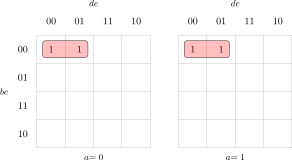
\includegraphics[width=292.1pt]{lect_3_kmap_5var}\caption{five variables}
\end{subfigure}
\caption{K-maps for five and six variables.}\label{fig:kmap56}
\end{figure}

\begin{figure}[htbp]
\centering
\ContinuedFloat
\begin{subfigure}[b]{294.8pt}\centering
  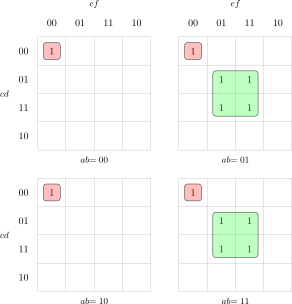
\includegraphics[width=292.8pt]{lect_3_kmap_6var}\caption{six variables}
\end{subfigure}
\caption[]{K-maps for five and six variables.}
\end{figure}

\section{Product-of-Sums Simplification}
A K-map also yields a minimal POS expression: \emph{group the 0s} instead of the 1s. There are two equivalent methods.

\paragraph{Method 1: simplify $F'$ and complement.} Group the 0s of $F$ (the 1s of $F'$) to obtain a minimal SOP for $F'$, then apply De~Morgan's theorem: if $F'=AB+C'D$, then $F=(AB+C'D)'=(A'+B')(C+D')$.

\paragraph{Method 2: direct.} For each group of 0s write a \emph{sum} term: a variable that is 0 over the group appears uncomplemented, a variable that is 1 appears complemented, and a variable that changes is eliminated. The function is the product of the sum terms.

\begin{example}{POS from a K-map}{pos}
Find the minimal POS of $F(A,B,C,D)=\Sm(0,1,2,5,8,9,10)$.

\textbf{Solution.} The 0s are at $m_3,m_4,m_6,m_7,m_{11},m_{12},m_{13},m_{14},m_{15}$ (\cref{fig:pos}). Group them as follows.
\begin{itemize}
  \item $m_{12},m_{13},m_{14},m_{15}$: $A=1,B=1$, giving the sum $(A'+B')$.
  \item $m_3,m_7,m_{11},m_{15}$: $C=1,D=1$, giving $(C'+D')$.
  \item $m_4,m_6,m_{12},m_{14}$: $B=1$, $D=0$, giving $(B'+D)$.
\end{itemize}
Hence $F=(A'+B')(C'+D')(B'+D)$.
\end{example}

\figw{188.2pt}{lect_3_kmap_pos}{Grouping the 0s of \cref{ex:pos}.}{fig:pos}

\section{NAND and NOR as Universal Gates}
The NAND gate ($(xy)'$) and the NOR gate ($(x+y)'$) are called \term{universal gates}: every other gate can be built from NANDs alone, or from NORs alone, so any digital circuit can be built from just one type of gate. This is useful because in many technologies NAND and NOR gates are smaller and faster than AND and OR gates. \Cref{fig:universal} shows the constructions; each follows from De~Morgan's theorem. A NAND with its inputs tied together is a NOT: $(xx)'=x'$. An AND is a NAND followed by a NAND used as an inverter. An OR is built from inverted inputs: $x+y=(x'y')'$. The NOR constructions are the duals.

\begin{figure}[htbp]
\centering
\begin{subfigure}[b]{130.0pt}\centering
  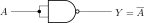
\includegraphics[width=128.0pt]{lect_3_nand_as_not}\caption{NOT}
\end{subfigure}
\hfill
\begin{subfigure}[b]{183.5pt}\centering
  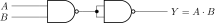
\includegraphics[width=181.5pt]{lect_3_nand_as_and}\caption{AND}
\end{subfigure}
\\[6pt]
\begin{subfigure}[b]{208.5pt}\centering
  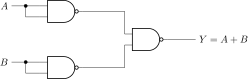
\includegraphics[width=206.5pt]{lect_3_nand_as_or}\caption{OR}
\end{subfigure}
\hfill
\begin{subfigure}[b]{144.9pt}\centering
  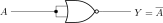
\includegraphics[width=142.9pt]{lect_3_nor_as_not}\caption{NOT}
\end{subfigure}
\\[6pt]
\begin{subfigure}[b]{187.2pt}\centering
  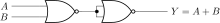
\includegraphics[width=185.2pt]{lect_3_nor_as_or}\caption{OR}
\end{subfigure}
\hfill
\begin{subfigure}[b]{204.7pt}\centering
  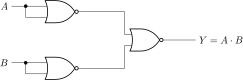
\includegraphics[width=202.7pt]{lect_3_nor_as_and}\caption{AND}
\end{subfigure}
\caption{Universal gates: NOT, AND and OR built from NAND gates only (top row) or from NOR gates only (bottom row).}\label{fig:universal}
\end{figure}

\subsection{Two-level NAND--NAND implementation of an SOP}
A minimal SOP expression is normally drawn as a two-level AND--OR circuit. Applying De~Morgan's theorem to the double complement converts it directly to \emph{two levels of NAND gates}:
\[
 F = AB + CD + E = \bigl((AB+CD+E)'\bigr)' = \bigl((AB)'\cdot(CD)'\cdot E'\bigr)'.
\]
The first level of NAND gates forms the complemented product terms $(AB)'$, $(CD)'$ and $E'$ (a single literal needs only an inverter); the second-level NAND gate then ORs the products. The circuits are shown in \cref{fig:twolevel}a and b. This is a very common implementation of the SOP obtained from a K-map.

\subsection{Two-level NOR--NOR implementation of a POS}
Dually, a POS expression, drawn as OR--AND, converts to \emph{two levels of NOR gates}:
\[
 F = (A+B)(C+D)E = \bigl(((A+B)(C+D)E)'\bigr)' = \bigl((A+B)' + (C+D)' + E'\bigr)'.
\]
This is the standard implementation when the expression was found by grouping 0s (\cref{fig:twolevel}c and d).

\begin{figure}[htbp]
\centering
\begin{subfigure}[b]{236.0pt}\centering
  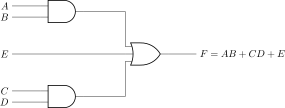
\includegraphics[width=234.0pt]{lect_3_two_level_sop}\caption{AND--OR}
\end{subfigure}
\\[6pt]
\begin{subfigure}[b]{236.0pt}\centering
  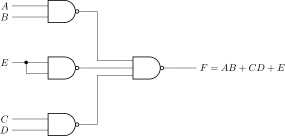
\includegraphics[width=234.0pt]{lect_3_two_level_sop_nand}\caption{NAND--NAND}
\end{subfigure}
\\[6pt]
\begin{subfigure}[b]{247.6pt}\centering
  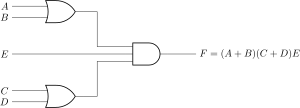
\includegraphics[width=245.6pt]{lect_3_two_level_pos}\caption{OR--AND}
\end{subfigure}
\caption{Two-level circuits: an SOP as AND--OR and as NAND--NAND (a, b); a POS as OR--AND and as NOR--NOR (c, d).}\label{fig:twolevel}
\end{figure}

\begin{figure}[htbp]
\centering
\ContinuedFloat
\begin{subfigure}[b]{247.6pt}\centering
  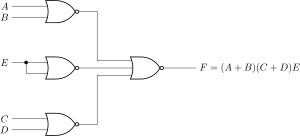
\includegraphics[width=245.6pt]{lect_3_two_level_pos_nor}\caption{NOR--NOR}
\end{subfigure}
\caption[]{Two-level circuits: an SOP as AND--OR and as NAND--NAND (a, b); a POS as OR--AND and as NOR--NOR (c, d).}
\end{figure}

\section{Exclusive-OR and Exclusive-NOR}
The \term{exclusive-OR} (XOR) function is 1 when its inputs \emph{differ}: $x\xor y = x'y+xy'$. The \term{exclusive-NOR} (XNOR, or \emph{equivalence}) is 1 when the inputs are \emph{equal}: $(x\xor y)' = xy+x'y'$. Both are fundamental in arithmetic and comparison circuits. Useful identities are
\[
 x\xor 0 = x,\qquad x\xor 1 = x',\qquad x\xor x = 0,\qquad x\xor x' = 1,
\]
and XOR is commutative and associative, $A\xor B = B\xor A$ and $(A\xor B)\xor C = A\xor(B\xor C)$, so that XOR of more than two variables is unambiguous. The symbols are shown in \cref{fig:xor}.

\begin{figure}[htbp]
\centering
\begin{subfigure}[b]{144.7pt}\centering
  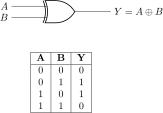
\includegraphics[width=142.7pt]{lect_3_xor_symbol}\caption{XOR}
\end{subfigure}
\hfill
\begin{subfigure}[b]{144.7pt}\centering
  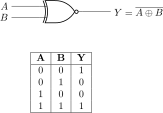
\includegraphics[width=142.7pt]{lect_3_xnor_symbol}\caption{XNOR}
\end{subfigure}
\caption{Symbols and truth tables of XOR and XNOR.}\label{fig:xor}
\end{figure}

\subsection{Odd and even functions}
The XOR of several variables is 1 when an \emph{odd} number of its inputs are 1; it is called the \term{odd function}. Its complement, the XNOR of several variables, is 1 when an \emph{even} number of the inputs are 1, and is called the \term{even function}. On a K-map these functions have a checkerboard pattern in which no two 1s are adjacent, so no simplification is possible (\cref{fig:oddeven}). For three variables
\[
 A\xor B\xor C = \Sm(1,2,4,7), \qquad (A\xor B\xor C)' = \Sm(0,3,5,6).
\]

\begin{figure}[htbp]
\centering
\begin{subfigure}[b]{183.5pt}\centering
  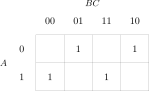
\includegraphics[width=181.5pt]{lect_3_kmap_odd}\caption{K-map of the odd function $A\xor B\xor C$}
\end{subfigure}
\hfill
\begin{subfigure}[b]{173.5pt}\centering
  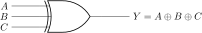
\includegraphics[width=171.5pt]{lect_3_logic_odd}\caption{logic diagram of the odd function}
\end{subfigure}
\\[6pt]
\begin{subfigure}[b]{183.5pt}\centering
  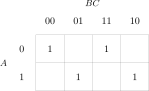
\includegraphics[width=181.5pt]{lect_3_kmap_even}\caption{K-map of the even function $(A\xor B\xor C)'$}
\end{subfigure}
\hfill
\begin{subfigure}[b]{173.5pt}\centering
  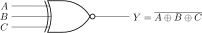
\includegraphics[width=171.5pt]{lect_3_logic_even}\caption{logic diagram of the even function}
\end{subfigure}
\caption{Odd and even functions of three variables: K-maps and logic diagrams.}\label{fig:oddeven}
\end{figure}

\section{Application: Parity Generation and Checking}\label{sec:parity}
XOR gates are ideal for detecting errors in data transmission. A \term{parity bit} is an extra bit appended to a message so that the total number of 1s is always even (\term{even parity}) or always odd (\term{odd parity}). \Cref{fig:parity-system} shows the system: a parity generator at the transmitter, the channel, and a parity checker at the receiver.

\figside{481.9pt}{lect_3_parity_system}{A parity system: the generator appends a parity bit; the checker at the receiver signals an error.}{fig:parity-system}

\paragraph{Even-parity generator.} For a 3-bit message $x,y,z$ the parity bit $P$ must make the number of 1s in $(x,y,z,P)$ even. This is true if and only if $P$ is the odd function of the message: $P=x\xor y\xor z$.

\paragraph{Even-parity checker.} The receiver computes $C = x\xor y\xor z\xor P$ from the four received bits; $C=0$ means that the number of 1s is even and no error is detected, whereas $C=1$ signals an error. A single-bit error always changes the parity and is detected; a double-bit error is not.

\begin{figure}[htbp]
\centering
\begin{subfigure}[b]{261.7pt}\centering
  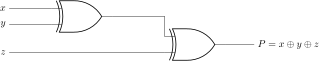
\includegraphics[width=259.7pt]{lect_3_logic_parity_generator}\caption{generator $P=x\xor y\xor z$}
\end{subfigure}
\\[6pt]
\begin{subfigure}[b]{320.8pt}\centering
  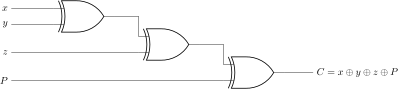
\includegraphics[width=318.8pt]{lect_3_logic_parity_checker}\caption{checker $C=x\xor y\xor z\xor P$}
\end{subfigure}
\caption{Even-parity generator and checker for a 3-bit message.}\label{fig:parity}
\end{figure}

\begin{lstlisting}[caption={Even-parity generator and checker in VHDL.},label={lst:parity}]
library ieee;
use ieee.std_logic_1164.all;

entity parity_generator is
  port (x, y, z : in  std_logic;
        p_even  : out std_logic);          -- parity bit for the even-parity scheme
end parity_generator;

architecture behavioral of parity_generator is
begin
  p_even <= x xor y xor z;                 -- 1 if the message has an odd number of 1s
end behavioral;

library ieee;
use ieee.std_logic_1164.all;

entity parity_checker is
  port (x, y, z, p_in : in  std_logic;     -- message and received parity bit
        err           : out std_logic);    -- 0 = no error detected, 1 = error detected
end parity_checker;

architecture behavioral of parity_checker is
begin
  err <= x xor y xor z xor p_in;           -- 1 if the total number of 1s is odd
end behavioral;
\end{lstlisting}

\begin{chaptersummary}
\begin{itemize}
  \item A \textbf{Karnaugh map} is a truth table arranged in Gray-code order so that adjacent squares differ in one variable. Groups of $2^k$ adjacent 1s eliminate $k$ variables.
  \item Group the 1s with \textbf{rectangles of size $2^k$}, as large as possible, allowing overlap and wrap-around; find all \textbf{prime implicants}, take the \textbf{essential} ones, then complete the cover with as few others as possible. A minimal SOP is not always unique.
  \item \textbf{Don't-cares} may be treated as 1 or as 0 to make larger groups.
  \item For a \textbf{minimal POS}, group the 0s and write sum terms (or simplify $F'$ and apply De~Morgan).
  \item \textbf{NAND} and \textbf{NOR} are universal; an SOP maps to a two-level \textbf{NAND--NAND} circuit, a POS to a two-level \textbf{NOR--NOR} circuit.
  \item \textbf{XOR} is the odd function and \textbf{XNOR} the even function; they form a checkerboard on the K-map and are the basis of \textbf{parity} generation and checking.
\end{itemize}
\end{chaptersummary}

\chapsec{Exercises}
\begin{exlist}
  \item Simplify $F(A,B,C)=\Sm(0,2,3,4,6)$. (a)~Construct the truth table. (b)~Draw the K-map and the groups. (c)~Write the minimal SOP. (d)~Draw the circuit with AND, OR and NOT gates.
  \item Simplify $F(w,x,y,z)=\Sm(0,1,2,7,8,9,10,15)$ with don't-cares $d(5,13)$. (a)~Draw the K-map, marking X squares. (b)~Find the minimal SOP, stating which don't-cares were used as 1s. (c)~Draw the circuit.
  \item Simplify $F(x,y,z)=\Sm(0,1,2,5,7)$ to a minimal \emph{POS}. (a)~Draw the K-map and plot the 0s. (b)~Find the minimal POS. (c)~Draw the two-level NOR--NOR circuit.
  \item \textbf{Prime and parity detector.} Design a 4-input circuit with inputs $A,B,C,D$ (binary number $ABCD$, $A$ the most significant bit) and two outputs. $F=1$ only when the input is a \emph{prime number} (0 and 1 are not prime). $G=1$ only when the number of 1s in the input is \emph{even}. Inputs 10--15 are not valid BCD and are don't-cares. (a)~Make one truth table for both outputs. (b)~Find the minimal SOP for $F$ and the minimal POS for $G$. (c)~Draw $F$ using only NAND gates and $G$ using only NOR gates.
  \item Find all prime implicants and all essential prime implicants of $F(w,x,y,z)=\Sm(0,2,3,5,7,8,10,11,13,15)$. Give all minimal SOP expressions.
  \item Simplify the following four-variable functions to minimal SOP: (a)~$F=\Sm(0,2,8,10)$; (b)~$F=\Sm(0,1,2,3,12,13,14,15)$; (c)~$F=\Sm(0,2,5,7,8,10,13,15)$.
  \item Convert the expression $F=AB+CD'+A'C'$ into (a)~a circuit with only NAND gates and (b)~a circuit with only NOR gates. Count the gates in each case.
  \item Show that the XOR operation is associative, $(A\xor B)\xor C = A\xor(B\xor C)$, by means of a truth table. How many 1s does the K-map of the 4-variable odd function $A\xor B\xor C\xor D$ contain?
  \item Design an \emph{odd}-parity generator for a 4-bit message $w,x,y,z$. Write the VHDL entity and architecture, and give the output for the messages \bin{0110}, \bin{0111} and \bin{1111}.
  \item The 7-bit ASCII code of the letter `A' is \bin{1000001}. What parity bit must be appended for (a)~even parity and (b)~odd parity? A receiver using even parity gets \bin{11000001} (parity bit first): is an error detected? Can the receiver tell which bit is wrong?
  \item Complete the 4-bit BCD to seven-segment decoder of Exercise~2.4 by finding minimal SOP expressions for segments $b$ and $c$ with the help of K-maps (outputs for inputs 10--15 are don't-cares).
\end{exlist}

\chapsec{Further Reading}
Karnaugh's original paper~\cite{karnaugh1953} is short and clear. McCluskey's tabular method~\cite{mccluskey1956} is the basis for computer-aided minimisation, and is covered in most digital-design textbooks, including Mano and Ciletti~\cite{mano2018} and Wakerly~\cite{wakerly2006}, the latter with an excellent discussion of timing hazards in two-level logic. Brown and Vranesic~\cite{brown2009} treat minimisation, NAND/NOR implementation and multilevel synthesis in depth.

\chapter{Number Representation and Arithmetic Circuits}\label{ch:arith}

\begin{objectives}
After studying this chapter you will be able to:
\begin{itemize}
  \item convert numbers among decimal, binary, octal and hexadecimal;
  \item represent signed integers in sign-magnitude, one's-complement and two's-complement form, and explain why two's complement is used in practice;
  \item add and subtract two's-complement numbers and detect arithmetic overflow;
  \item design half adders, full adders, ripple-carry adders and adder/subtractor circuits, and describe them in VHDL;
  \item explain the delay problem of the ripple-carry adder and design a carry-lookahead adder using generate and propagate signals;
  \item multiply unsigned numbers with an array multiplier;
  \item represent fractions in fixed-point and IEEE~754 floating-point formats, and decimal digits and characters in BCD and ASCII.
\end{itemize}
\end{objectives}

\section{Positional Number Systems}\label{sec:numsys}
Section~\ref{sec:adc} showed that a binary string can represent a quantity. In a positional system with radix $r$ the value of the digit string $d_{n-1}\cdots d_1d_0.\,d_{-1}d_{-2}\cdots$ is $\sum_i d_i r^{\,i}$, with negative $i$ for the fraction. Four radices matter in digital design:
\begin{itemize}
  \item \textbf{Binary} ($r=2$), digits 0 and 1; each digit is a \term{bit}, and a group of eight bits is a \term{byte}.
  \item \textbf{Octal} ($r=8$), digits 0--7; one octal digit stands for exactly three bits.
  \item \textbf{Decimal} ($r=10$), the system used by people.
  \item \textbf{Hexadecimal} ($r=16$), digits 0--9 and A--F (A$=10$, \dots, F$=15$); one hex digit stands for exactly four bits. It is the usual compact way of writing binary values.
\end{itemize}
\Cref{tab:radix} lists the first values. The binary--octal--hex conversions are trivial because $8=2^3$ and $16=2^4$: group the bits in threes or fours starting at the binary point, and replace each group by its digit.

\begin{table}[htbp]
\centering
\small
\caption{The numbers 0 to 16 in four radices.}
\label{tab:radix}
\begin{tabular}{@{}cccc@{\hspace{2.5em}}cccc@{}}
\toprule
Dec & Binary & Oct & Hex & Dec & Binary & Oct & Hex\\
\midrule
0&00000&00&0 & 9 &01001&11&9\\
1&00001&01&1 & 10&01010&12&A\\
2&00010&02&2 & 11&01011&13&B\\
3&00011&03&3 & 12&01100&14&C\\
4&00100&04&4 & 13&01101&15&D\\
5&00101&05&5 & 14&01110&16&E\\
6&00110&06&6 & 15&01111&17&F\\
7&00111&07&7 & 16&10000&20&10\\
8&01000&10&8 & &&&\\
\bottomrule
\end{tabular}
\end{table}

\subsection{Converting from decimal}
To convert the \emph{integer part} to radix $r$, divide repeatedly by $r$ and collect the remainders; the first remainder is the least significant digit. To convert the \emph{fractional part}, multiply repeatedly by $r$ and collect the integer parts; the first is the most significant fractional digit.

\begin{example}{Radix conversion}{radix}
Convert $156_{10}$ to binary, hexadecimal and octal, and convert $0.6875_{10}$ to binary.

\textbf{Solution.} Dividing 156 by 2 repeatedly gives remainders $0,0,1,1,1,0,0,1$ (least significant first), so $156 = \bin{10011100}_2$. Grouping in fours gives $\bin{1001}\,\bin{1100}=9\mathrm{C}_{16}$, and grouping in threes ($\bin{010}\,\bin{011}\,\bin{100}$) gives $234_8$. Check: $2\cdot64+3\cdot8+4=156$.
For the fraction: $0.6875\times2=1.375\to1$; $0.375\times2=0.75\to0$; $0.75\times2=1.5\to1$; $0.5\times2=1.0\to1$, so $0.6875=\bin{0.1011}_2$.
\end{example}

\section{Signed Integer Representations}\label{sec:signed}
To represent negative numbers in binary, the most significant bit (MSB) is used as a \term{sign bit}: 0 means positive and 1 means negative (\cref{fig:msb}). Three schemes differ in how the remaining bits represent a negative value.

\figw{213.3pt}{lect_4_8bit_msb_lsb}{An 8-bit signed number: the MSB is the sign bit, the LSB is bit 0.}{fig:msb}

\paragraph{Sign-magnitude.} The remaining $n-1$ bits hold the magnitude. The range is $\pm(2^{n-1}-1)$ and there are \emph{two zeros}, $\bin{0000}$ ($+0$) and $\bin{1000}$ ($-0$). Arithmetic is awkward, since the signs and magnitudes must be compared first.

\paragraph{One's complement.} Positive numbers are as in sign-magnitude; a negative number is obtained by \emph{inverting every bit} of the positive number: $+5=\bin{0101}$, $-5=\bin{1010}$. There are again two zeros ($\bin{0000}$ and $\bin{1111}$). Addition requires an \emph{end-around carry}: the carry out of the MSB is added back to the result.

\paragraph{Two's complement.} A negative number is obtained by inverting all bits and \emph{adding 1}: $+5=\bin{0101}\to\bin{1010}\to\bin{1011}=-5$. There is only one zero, and the range is asymmetric: $-2^{n-1}$ to $2^{n-1}-1$. The value of an $n$-bit two's-complement number is
\begin{equation}
  V = -d_{n-1}\,2^{\,n-1} + \sum_{i=0}^{n-2} d_i\,2^{\,i}.
  \label{eq:twos}
\end{equation}
Hence $\bin{10110101} = -128+32+16+4+1=-75$. \Cref{tab:signed} compares the three schemes for 4-bit numbers.

\begin{table}[htbp]
\centering
\small
\caption{Four-bit signed numbers in the three representations.}
\label{tab:signed}
\begin{tabular}{@{}rccc@{\hspace{3em}}rccc@{}}
\toprule
Dec & Sign-mag. & 1's comp. & 2's comp. & Dec & Sign-mag. & 1's comp. & 2's comp.\\
\midrule
$+7$&0111&0111&0111 & $-0$&1000&1111&---\\
$+6$&0110&0110&0110 & $-1$&1001&1110&1111\\
$+5$&0101&0101&0101 & $-2$&1010&1101&1110\\
$+4$&0100&0100&0100 & $-3$&1011&1100&1101\\
$+3$&0011&0011&0011 & $-4$&1100&1011&1100\\
$+2$&0010&0010&0010 & $-5$&1101&1010&1011\\
$+1$&0001&0001&0001 & $-6$&1110&1001&1010\\
$+0$&0000&0000&0000 & $-7$&1111&1000&1001\\
    &&&              & $-8$&---&---&1000\\
\bottomrule
\end{tabular}
\end{table}

\begin{example}{Two's-complement conversions}{twos}
(a)~Represent $-75$ as an 8-bit two's-complement number, in binary and hexadecimal. (b)~Find the decimal value of $\bin{1011\,0101}$. (c)~Extend $\bin{1011}$ ($-5$) to 8 bits.

\textbf{Solution.} (a)~$+75=\bin{0100\,1011}$. Invert: $\bin{1011\,0100}$. Add 1: $\bin{1011\,0101}=\mathrm{B5}_{16}$. (b)~Using \cref{eq:twos}, $-128+32+16+4+1=-75$; this is indeed the number found in~(a). (c)~To widen a two's-complement number, \term{sign-extend} it by copying the sign bit into the new upper bits: $\bin{1111\,1011}$, which is again $-5$ ($-128+64+32+16+8+2+1=-5$).
\end{example}

\begin{keypoint}[Why two's complement?]
Two's complement has a single zero, a simple negation (invert and add 1), and, above all, \emph{the same adder circuit adds signed and unsigned numbers}: subtraction is just addition of the negated operand. This is why every modern processor uses it.
\end{keypoint}

\section{Arithmetic and Overflow}\label{sec:overflow}
\Cref{ex:addrep} shows the calculation $4+(-3)$ in the three representations.

\begin{example}{$4+(-3)$ in the three systems}{addrep}
\textbf{Sign-magnitude.} $+4=\bin{0100}$, $-3=\bin{1011}$. The signs differ, so subtract the smaller magnitude from the larger: $\bin{100}-\bin{011}=\bin{001}$, with the sign of the larger magnitude (positive): $\bin{0001}=+1$.\\
\textbf{One's complement.} $-3=\bin{1100}$. $\bin{0100}+\bin{1100}=\bin{1\,0000}$. The end-around carry gives $\bin{0000}+1=\bin{0001}=+1$.\\
\textbf{Two's complement.} $-3=\bin{1101}$. $\bin{0100}+\bin{1101}=\bin{1\,0001}$. Discarding the carry-out gives $\bin{0001}=+1$.
\end{example}

If the true result of an operation lies outside the range of the representation, \term{arithmetic overflow} occurs and the result is wrong. With $n$ bits the range for signed numbers is $-2^{n-1}$ to $2^{n-1}-1$. For example, in 4 bits $(+7)+(+2)=+9$ computes as $\bin{0111}+\bin{0010}=\bin{1001}$, which reads as $-7$. Similarly $(-7)+(-2)=\bin{1001}+\bin{1110}=\bin{1\,0111}$, which after discarding the carry reads as $+7$. Two facts make detection easy. First, overflow \emph{cannot occur when the operands have different signs}. Second, when it does occur, the carry into the sign bit differs from the carry out of it.

\begin{keypoint}[Overflow rule for two's complement]
Let $c_{n-1}$ be the carry into the sign-bit position and $c_n$ the carry out of it. Overflow occurs if and only if
\[
  \text{overflow} = c_{n-1}\xor c_n .
\]
\end{keypoint}

In the first example, $c_4=0$ and $c_3=1$; in the second, $c_4=1$ and $c_3=0$. In both cases the two carries differ, so overflow is signalled.

\section{Adders}\label{sec:adders}
\subsection{Half adder and full adder}
The half adder of \cref{ex:half-adder} adds two bits. To add multi-bit numbers we need to include the carry arriving from the lower position: a \term{full adder} (FA) adds three bits, $A$, $B$ and $C_{in}$, and produces a sum $S$ and carry-out $C_{out}$ (\cref{tab:fa}). From the truth table
\begin{equation}
 S = A\xor B\xor C_{in}, \qquad C_{out} = AB + C_{in}(A\xor B).
 \label{eq:fa}
\end{equation}
The carry output is the \emph{majority} function of the three inputs, so it also equals $AB + AC_{in} + BC_{in}$.

\begin{table}[htbp]
\centering
\caption{Truth table of the full adder.}
\label{tab:fa}
\begin{tabular}{ccc|cc}
\toprule
$A$&$B$&$C_{in}$&$C_{out}$&$S$\\ \midrule
0&0&0&0&0\\0&0&1&0&1\\0&1&0&0&1\\0&1&1&1&0\\
1&0&0&0&1\\1&0&1&1&0\\1&1&0&1&0\\1&1&1&1&1\\ \bottomrule
\end{tabular}
\end{table}

Equation~\eqref{eq:fa} shows that a full adder can be built from \emph{two half adders and an OR gate}: the first half adder adds $A$ and $B$ giving $S_1=A\xor B$ and $C_1=AB$; the second adds $S_1$ and $C_{in}$ giving $S=S_1\xor C_{in}$ and $C_2=S_1C_{in}$; and $C_{out}=C_1+C_2$ (\cref{fig:fa}). \Cref{lst:fa} is the corresponding \emph{structural} VHDL description, in which a design is written as a set of component instances connected by signals; it uses the half-adder entity of \cref{lst:half-adder}.

\begin{figure}[htbp]
\centering
\begin{subfigure}[b]{324.2pt}\centering
  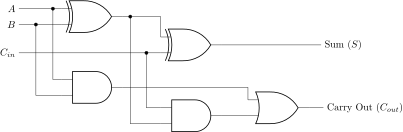
\includegraphics[width=322.2pt]{lect_4_circuit_full_adder}\caption{gate-level circuit}
\end{subfigure}
\\[6pt]
\begin{subfigure}[b]{299.2pt}\centering
  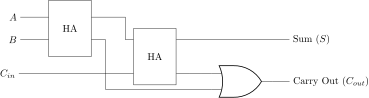
\includegraphics[width=297.2pt]{lect_4_circuit_full_adder_from_ha}\caption{from two half adders}
\end{subfigure}
\caption{Two implementations of the full adder.}\label{fig:fa}
\end{figure}

\vhdlfile[firstline=1, lastline=57]{../vhdl/full_adder.vhd}{Structural VHDL of the full adder, built from two half-adder components.}{lst:fa}

\subsection{Ripple-carry adder}
To add two $n$-bit numbers we cascade $n$ full adders: the carry-out of stage $i$ becomes the carry-in of stage $i+1$. The first carry-in $C_0$ is 0 for ordinary addition. \Cref{fig:ripple} shows a 4-bit \term{ripple-carry adder}, so called because the carry ``ripples'' from the least significant to the most significant stage. \Cref{lst:ripple} describes it in VHDL using a \code{std_logic_vector}, which is an array of bits written with an index range such as \code{(3 downto 0)}, and an internal vector of carries.

\figw{301.8pt}{lect_4_circuit_ripple_adder}{A 4-bit ripple-carry adder built from four full adders.}{fig:ripple}

\vhdlfile{../vhdl/ripple_adder_4bit.vhd}{Structural VHDL of a 4-bit ripple-carry adder.}{lst:ripple}

\Cref{fig:sim-ra} shows a ModelSim simulation of this adder using a testbench with assertions: $0+0$, $1+1$, $15+1$ (carry out, sum $0000$), $15+15+1$ (sum $1111$, carry out 1) and $5+3$ (sum $1000$). The testbenches of this chapter, in the style of \cref{lst:tb}, are provided with the book's source files.

\begin{figure}[htbp]
\centering
\wavesplit{lect_4_sim_result_RA}{3}\vspace{4pt}
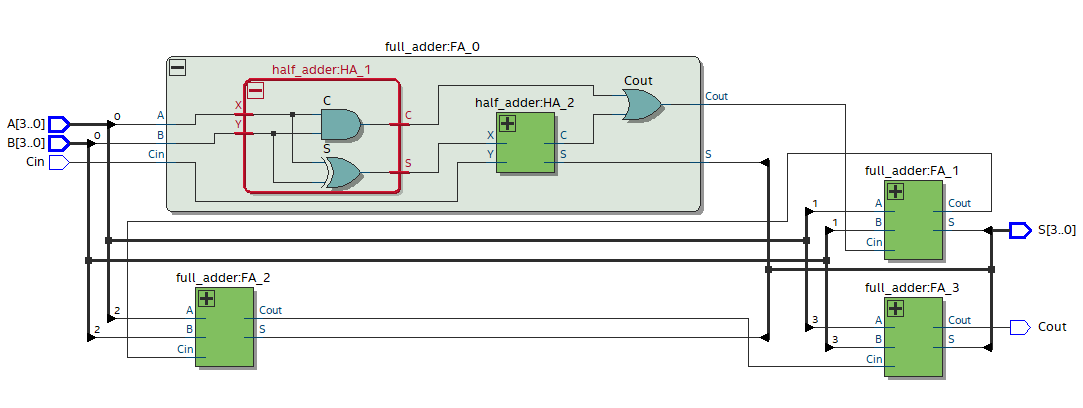
\includegraphics[width=\linewidth]{lect_4_rtl_viewer_RA}
\caption{Ripple-carry adder: ModelSim simulation of the testbench (top) and the RTL viewer schematic produced by Quartus (bottom), author's screenshots.}
\label{fig:sim-ra}
\end{figure}

\subsection{Adder/subtractor}
Since $A-B = A+(-B) = A+\NOT{B}+1$ in two's complement, the same adder performs subtraction if the bits of $B$ are inverted and the initial carry-in is 1. An XOR gate works as a \emph{controllable inverter}: $B_i\xor 0=B_i$ and $B_i\xor 1=B_i'$. With a control input $\mathit{sub}$ ($0$ = add, $1$ = subtract) connected both to the XOR gates and to $C_0$ we obtain the adder/subtractor of \cref{fig:addsub}. When $\mathit{sub}=0$ the circuit computes $A+B$, and when $\mathit{sub}=1$ it computes $A+\NOT{B}+1=A-B$. The overflow signal is $c_{n-1}\xor c_n$.

\figw{245.5pt}{lect_4_circuit_adder_subtractor}{A 4-bit adder/subtractor. The XOR gates conditionally complement $B$, and the control input is also the initial carry.}{fig:addsub}

\vhdlfile{../vhdl/adder_subtractor_4bit.vhd}{VHDL of the 4-bit adder/subtractor, reusing the ripple-carry adder.}{lst:addsub}

\begin{figure}[htbp]
\centering
\wavesplit{lect_4_sim_result_AS}{4}
\caption{ModelSim simulation of the adder/subtractor: $5+3=8$, $5-3=2$, $3-5=-2$ ($\bin{1110}$), $7+2$ (overflow, $\bin{1001}$) and $-8-1$ (overflow, $\bin{0111}$). Author's screenshot.}
\label{fig:sim-as}
\end{figure}

\section{The Carry Delay and the Carry-Lookahead Adder}\label{sec:cla}
\subsection{Delay of the ripple-carry adder}
The \term{critical path}, the longest delay between an input change and a stable output, of a ripple-carry adder passes through the carry chain. The worst case, for example $\bin{1111}+\bin{0001}$, requires the carry generated in the first stage to travel through every later stage. If each full adder adds two gate delays on the carry path, an $n$-bit adder has a delay of about $2n$ gate delays, so a 16-bit adder needs about $32$ gate delays (\cref{fig:rcdelay}). The delay grows linearly with $n$, which is unacceptable in a fast processor.

\figw{353.1pt}{lect_4_ripple_carry_delay}{The carry must ripple through every stage in the worst case.}{fig:rcdelay}

\subsection{Generate and propagate}
A \term{carry-lookahead adder} (CLA) computes all the carries in parallel directly from the inputs, which removes the long dependency chain. The key is to re-express the full adder in terms of two signals for each bit position $i$:
\begin{itemize}
  \item the \term{generate} signal $G_i = A_iB_i$: stage $i$ produces a carry by itself, regardless of its carry-in;
  \item the \term{propagate} signal $P_i = A_i\xor B_i$: stage $i$ passes its carry-in on to its carry-out.
\end{itemize}
Then
\begin{equation}
  S_i = P_i\xor C_i, \qquad C_{i+1} = G_i + P_iC_i .
  \label{eq:gp}
\end{equation}
Substituting repeatedly removes the dependence on the previous carry:
\begin{align*}
 C_1 &= G_0 + P_0C_0,\\
 C_2 &= G_1 + P_1G_0 + P_1P_0C_0,\\
 C_3 &= G_2 + P_2G_1 + P_2P_1G_0 + P_2P_1P_0C_0,\\
 C_4 &= G_3 + P_3G_2 + P_3P_2G_1 + P_3P_2P_1G_0 + P_3P_2P_1P_0C_0 .
\end{align*}
Each carry is a two-level AND--OR expression of the $P_i$, $G_i$ and $C_0$ only, and all four are computed at the same time (\cref{fig:cla4}).

\figw{364.8pt}{lect_4_circuit_cla_4bit}{Block diagram of a 4-bit carry-lookahead adder: a P/G generator for each bit, the lookahead logic, and sum XOR gates.}{fig:cla4}

\Cref{lst:cla-logic} is the lookahead logic block in VHDL and \cref{lst:cla4} is the top-level design, which instantiates the P/G units, the lookahead block and the sum gates.

\vhdlfile{../vhdl/cla_logic.vhd}{Carry-lookahead logic block of the 4-bit CLA.}{lst:cla-logic}

\vhdlfile{../vhdl/cla_4bit_adder.vhd}{Top level of the 4-bit carry-lookahead adder.}{lst:cla4}

\subsection{Hierarchical lookahead}
The fan-in (number of inputs) of the gates in a lookahead circuit grows with the word length, so a single-level CLA is impractical for 16 or 32 bits. The remedy is to build a \emph{hierarchy}: a 16-bit adder is made of four 4-bit CLA blocks, and a second-level lookahead unit computes the carries between the blocks. Each 4-bit block supplies a block-propagate and a block-generate signal:
\begin{align*}
 P^*_0 &= P_3P_2P_1P_0, & G^*_0 &= G_3 + P_3G_2 + P_3P_2G_1 + P_3P_2P_1G_0,
\end{align*}
and similarly $P^*_1,G^*_1$ for bits 4--7, $P^*_2,G^*_2$ for bits 8--11 and $P^*_3,G^*_3$ for bits 12--15. The block carries follow the same pattern as the bit carries:
\begin{align*}
 c_4 &= G^*_0 + P^*_0c_0,\\
 c_8 &= G^*_1 + P^*_1G^*_0 + P^*_1P^*_0c_0,\\
 c_{12} &= G^*_2 + P^*_2G^*_1 + P^*_2P^*_1G^*_0 + P^*_2P^*_1P^*_0c_0 .
\end{align*}
The structure is shown in \cref{fig:cla16}.

\figside{501.5pt}{lect_4_16-bit_cla}{A 16-bit adder with four 4-bit carry-lookahead blocks and a second-level lookahead unit.}{fig:cla16}

\begin{example}{Delay comparison for 16 bits}{cladelay}
Take one gate delay as $t$.

\textbf{Ripple-carry:} the carry passes through 16 full adders at $2t$ each: $16\times2t=32t$.

\textbf{Hierarchical CLA:} (1)~all $P_i$ and $G_i$: $1t$; (2)~block $P^*$ and $G^*$: $2t$; (3)~second-level lookahead gives $c_4,c_8,c_{12}$: $2t$; (4)~the carries inside each block: $2t$; (5)~the sum bits $S_i=P_i\xor C_i$: $1t$. The total is $1+2+2+2+1 = 8t$, four times faster than the ripple-carry adder, at the price of more gates.
\end{example}

\begin{figure}[htbp]
\centering
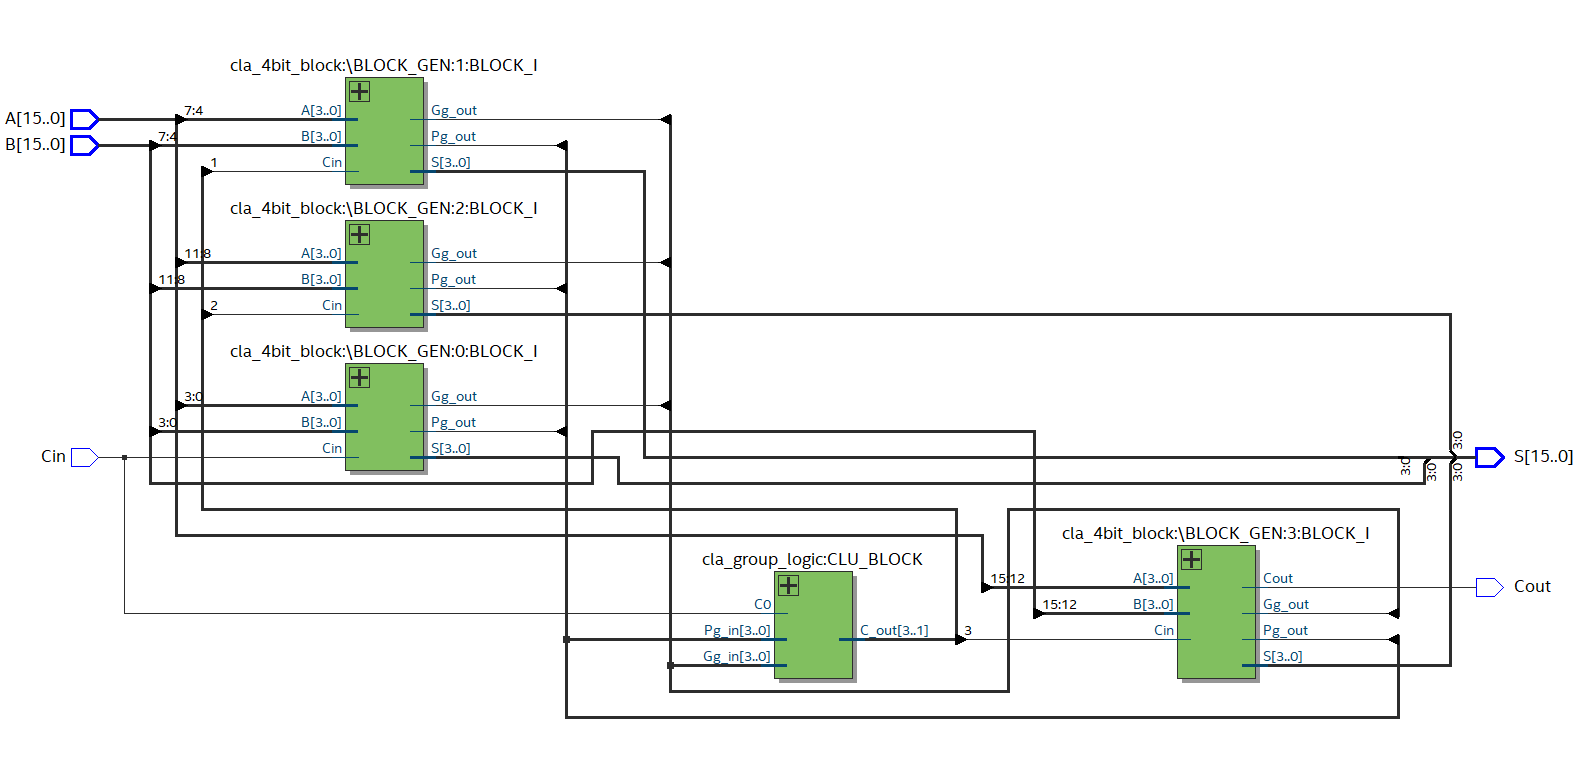
\includegraphics[width=\linewidth]{lect_4_rtl_viewer_cla_16bit}\\[4pt]
\wavesplit{lect_4_sim_result_cla_16bit}{3}
\caption{16-bit carry-lookahead adder: RTL viewer (top) and ModelSim simulation (bottom). Author's screenshots. The VHDL files \code{cla_4bit_block}, \code{cla_group_logic} and \code{cla_16bit_adder} accompany the book.}
\label{fig:cla16-sim}
\end{figure}

\section{Multiplication}\label{sec:mult}
Binary multiplication is a process of adding \emph{partial products}. Because each multiplier bit is 0 or 1, each partial product is either zero or a copy of the multiplicand, shifted to the position of the multiplier bit.

\begin{example}{Multiplying $1101\times1011$}{mult}
Multiply $A=\bin{1101}\ (13)$ by $B=\bin{1011}\ (11)$.
\begin{center}\ttfamily
\begin{tabular}{@{}r@{}}
\phantom{000}1101\\
$\times$\ \ 1011\\ \hline
\phantom{000}1101\\
\phantom{00}11010\\
\phantom{0}000000\\
1101000\\ \hline
10001111
\end{tabular}
\end{center}
The partial products are $A\times B_0$, $A\times B_1$ (shifted one place), and so on; adding them, $\bin{1101}+\bin{11010}+\bin{000000}+\bin{1101000}=13+26+0+104=143=\bin{10001111}$. The product of two 4-bit numbers needs up to 8 bits.
\end{example}

An \term{array multiplier} implements this directly. An AND gate forms each bit of the partial products, $A_iB_j$, and an array of adders adds them with the correct shifts. For a $4\times4$ multiplier (\cref{fig:mult4}) we need 16 AND gates and 12 adders (3 half adders and 9 full adders in the design of \cref{lst:mult}). \Cref{lst:mult} also shows the VHDL \code{generate} statement, which replicates hardware: here it creates the 16 AND gates.

\figw{410.0pt}{lect_4_multiplier_4x4}{A $4\times4$ array multiplier: partial products are formed by AND gates and summed by rows of adders.}{fig:mult4}

\vhdlfile[firstline=1, lastline=62]{../vhdl/multiplier_4x4.vhd}{VHDL of the $4\times4$ array multiplier (first part: declarations, partial products and the first adder row). The remaining rows follow the same pattern.}{lst:mult}

\begin{figure}[htbp]
\centering
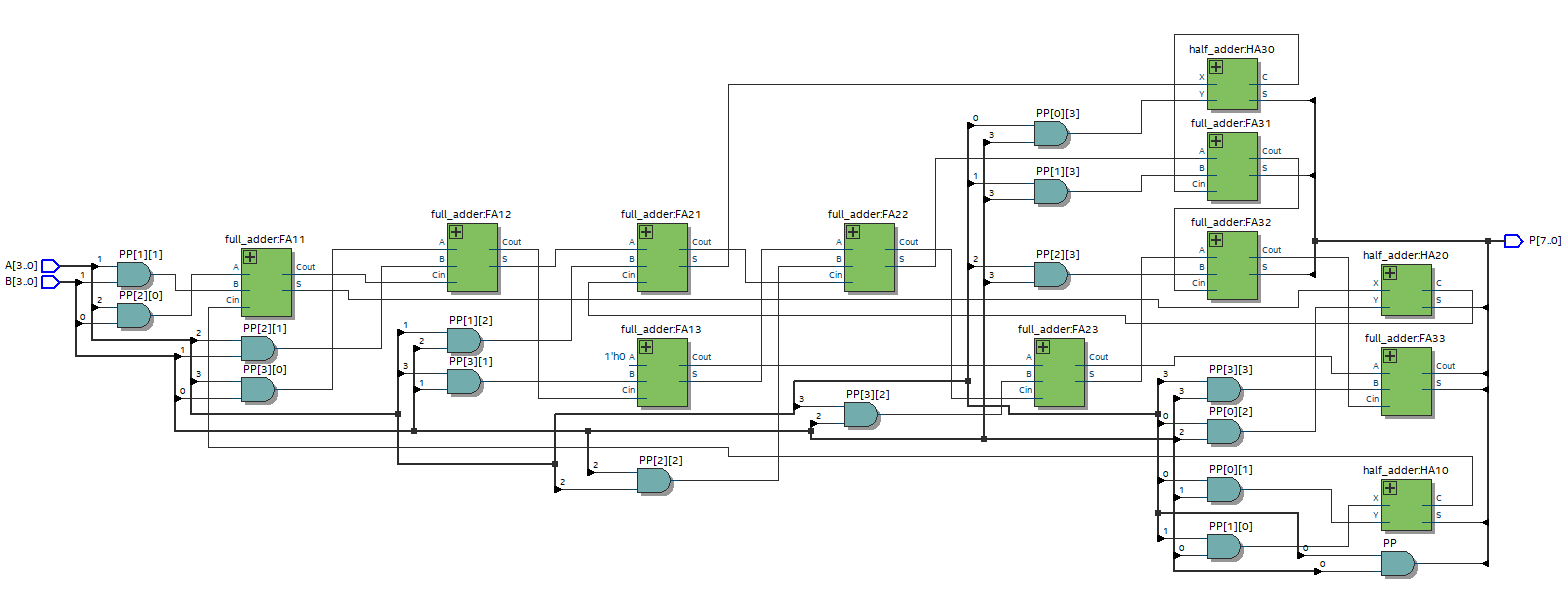
\includegraphics[width=\linewidth]{lect_4_rtl_viewer_mul_4x4}\\[4pt]
\wavesplit{lect_4_sim_result_mul_4x4}{3}
\caption{$4\times4$ multiplier: RTL viewer (top) and ModelSim simulation (bottom). Author's screenshots.}
\label{fig:mult-sim}
\end{figure}

\section{Fractions and Floating Point}\label{sec:fixfloat}
\subsection{Fixed-point numbers}
A \term{fixed-point} number represents a fraction with a fixed number of bits for the integer and fractional parts; the binary point is implicit. The notation $Qn.m$ means $n$ integer bits and $m$ fractional bits (unsigned unless stated otherwise); the resolution is $2^{-m}$ and the range $0$ to $2^n-2^{-m}$. Fixed-point arithmetic uses ordinary integer hardware, so it is fast, small and low-power, but the range and precision are limited and the designer must choose the format carefully to avoid overflow and loss of precision.

\begin{example}{Fixed-point conversion}{fixed}
Represent $6.75_{10}$ in $Q4.4$ format (8 bits).

\textbf{Solution.} The integer part is $6=\bin{0110}$. The fraction: $0.75\times2=1.5\to1$; $0.5\times2=1.0\to1$; then $0, 0$. So $0.75=\bin{.1100}$ and the number is $\bin{0110.1100}=\bin{01101100}$. Check: $4+2+0.5+0.25=6.75$.
\end{example}

\subsection{Floating-point numbers (IEEE~754)}
Floating point represents a number as a sign, a significand (mantissa) and a power of two, much like scientific notation, and gives a huge dynamic range with a fixed word length. The \term{IEEE~754} standard~\cite{ieee754} defines the formats; the 32-bit \emph{single precision} format (\cref{fig:fp32}) has
\begin{itemize}
  \item a \textbf{sign} bit $S$ (0 positive, 1 negative);
  \item an 8-bit \textbf{exponent} $E$ in \emph{excess-127} form (true exponent $=E-127$);
  \item a 23-bit \textbf{fraction} $M$. A normalised number has the form $1.M$; the leading 1 is not stored (the \term{hidden bit}), which gives 24 bits of precision.
\end{itemize}
\begin{equation}
  V = (-1)^S\times(1.M)_2\times2^{\,E-127}.
  \label{eq:ieee}
\end{equation}
The exponent values $E=0$ and $E=255$ are reserved for zero and subnormal numbers, and for infinity and \emph{not-a-number} (NaN). Normal single-precision numbers range from about $1.2\times10^{-38}$ to $3.4\times10^{38}$ with about seven significant decimal digits. A useful discussion of the pitfalls of floating-point arithmetic is given by Goldberg~\cite{goldberg1991}.

\figside{448.1pt}{lect_4_floating_point_32bit}{The IEEE~754 single-precision format.}{fig:fp32}

\begin{example}{Encoding $3.5$ and $-6.25$}{ieee}
\textbf{$3.5$.} $3.5=\bin{11.1}=\bin{1.11}\times2^1$. $S=0$; $E=1+127=128=\bin{10000000}$; $M=\bin{11}$ followed by 21 zeros. The word is $\bin{0\ 10000000\ 11000000000000000000000}$, or $\mathrm{40600000}_{16}$.

\textbf{$-6.25$.} $6.25=\bin{110.01}=\bin{1.1001}\times2^2$. $S=1$; $E=2+127=129=\bin{10000001}$; $M=\bin{1001}$ then zeros. The word is $\bin{1\ 10000001\ 10010000000000000000000}=\mathrm{C0C80000}_{16}$.
\end{example}

\section{Codes for Decimal Digits and Characters}\label{sec:codes}
\paragraph{Binary-coded decimal (BCD).} \term{BCD} encodes each decimal digit in four bits: $0=\bin{0000}$ up to $9=\bin{1001}$; the codes $\bin{1010}$ to $\bin{1111}$ are unused (and are natural don't-cares in a K-map). For example $78_{10}=\bin{0111\,1000}_{\mathrm{BCD}}$, whereas the binary value of 78 is $\bin{0100\,1110}$. BCD wastes some codes and needs special adders (\cref{ch:blocks}), but it makes conversion to a display trivial, which is why it is used in calculators and digital clocks (\cref{fig:bcdclock}).

\figw{218.6pt}{lect_4_bcd_clock}{BCD digits drive the displays of a digital clock.}{fig:bcdclock}

\paragraph{ASCII.} The \term{American Standard Code for Information Interchange}~\cite{ansix34} assigns 7-bit codes to 128 characters: codes 0--31 (and 127) are non-printing control characters, and codes 32--126 are the space, punctuation, the digits and the upper- and lower-case letters. Most modern systems use 8-bit extensions, and ASCII is the first 128 code points of Unicode and UTF-8. Some codes are listed in \cref{tab:ascii}. Note that lower-case letters differ from the corresponding upper-case letters by exactly one bit (bit~5: $\mathrm{a}=\mathrm{A}+32$), and that the digit characters have the decimal value in their low nibble ($\texttt{'7'}=\mathrm{37}_{16}$).

\begin{table}[htbp]
\centering
\caption{Example ASCII codes.}
\label{tab:ascii}
\begin{tabular}{lccc@{\hspace{3em}}lccc}
\toprule
Char & Dec & Hex & Binary & Char & Dec & Hex & Binary\\ \midrule
A & 65 & 41 & 0100\,0001 & 0 & 48 & 30 & 0011\,0000\\
B & 66 & 42 & 0100\,0010 & 1 & 49 & 31 & 0011\,0001\\
a & 97 & 61 & 0110\,0001 & space & 32 & 20 & 0010\,0000\\
b & 98 & 62 & 0110\,0010 & ! & 33 & 21 & 0010\,0001\\
\bottomrule
\end{tabular}
\end{table}

\begin{chaptersummary}
\begin{itemize}
  \item Binary, octal and hexadecimal are related by grouping bits in threes and fours. Convert from decimal by repeated division (integer part) and multiplication (fraction).
  \item \textbf{Two's complement} is the standard signed representation: negate by inverting and adding 1; range $-2^{n-1}\dots2^{n-1}-1$; one zero; the same adder works for signed and unsigned numbers. Overflow $=c_{n-1}\xor c_n$.
  \item A \textbf{full adder} computes $S=A\xor B\xor C_{in}$ and $C_{out}=AB+C_{in}(A\xor B)$. $n$ of them form a \textbf{ripple-carry adder}, whose delay grows linearly with $n$.
  \item The \textbf{adder/subtractor} uses XOR gates to complement $B$ and the control signal as the first carry-in.
  \item The \textbf{carry-lookahead adder} uses $G_i=A_iB_i$ and $P_i=A_i\xor B_i$ to compute all carries in parallel; a hierarchical design reduces a 16-bit delay from about $32t$ to about $8t$.
  \item An \textbf{array multiplier} forms partial products with AND gates and adds them with an array of adders.
  \item \textbf{Fixed-point} ($Qn.m$) is cheap but has limited range; \textbf{IEEE~754} single precision is $(-1)^S\,1.M\times2^{E-127}$. \textbf{BCD} and \textbf{ASCII} encode digits and characters.
\end{itemize}
\end{chaptersummary}

\chapsec{Exercises}
\begin{exlist}
  \item \textbf{Number conversion.} (a)~Convert the decimal number $-75$ to an 8-bit two's-complement binary number and to hexadecimal. (b)~What is the decimal value of the 8-bit two's-complement number $\bin{1011\,0101}$?
  \item \textbf{Two's-complement arithmetic.} Let $A=\bin{0110\,1001}$ and $B=\bin{1101\,0110}$ be 8-bit two's-complement numbers. (a)~Calculate $A+B$. Is there an overflow? (b)~Calculate $A-B$ (as $A+(-B)$). Is there an overflow?
  \item \textbf{Adder delay.} (a)~What is the approximate worst-case delay of a 16-bit ripple-carry adder if each full adder contributes two gate delays on the carry path? (b)~Define the propagate $P_i$ and generate $G_i$ signals of a carry-lookahead adder and explain why they are useful.
  \item \textbf{8-bit adder in VHDL.} Using the entity \code{ripple_adder_4bit} of \cref{lst:ripple} as a component, write the structural VHDL of an 8-bit ripple-carry adder with inputs \code{A, B : std_logic_vector(7 downto 0)} and \code{Cin}, and outputs \code{S} and \code{Cout}. How many internal signals do you need to connect the two blocks?
  \item Convert (a)~$\bin{1011\,0110}_2$ to decimal and hexadecimal; (b)~$\mathrm{A7}_{16}$ to binary and decimal; (c)~$725_8$ to binary and decimal; (d)~$0.8125_{10}$ to binary.
  \item Write $+19$, $-19$ and $-32$ as 6-bit two's-complement numbers. What is the range of 6-bit two's-complement numbers?
  \item Perform the following in 5-bit two's complement, and state whether overflow occurs: (a)~$9+7$; (b)~$(-9)+(-8)$; (c)~$12-5$.
  \item Show that for two's-complement addition, $S=A+B$, overflow also occurs if and only if the two operands have the same sign and the sign of the result is different, i.e.\ $V = A_{n-1}B_{n-1}S_{n-1}' + A_{n-1}'B_{n-1}'S_{n-1}$.
  \item Show from the truth table that $C_{out}=AB+AC_{in}+BC_{in}$ for the full adder, and derive the same expression from \cref{eq:fa}. Draw the corresponding two-level circuit.
  \item For $A=\bin{1011}$, $B=\bin{0110}$ and $C_0=1$, compute $G_i$, $P_i$, $C_1,\dots,C_4$ and $S_3S_2S_1S_0$ using the carry-lookahead equations. Verify the result by ordinary addition.
  \item Multiply $\bin{1011}\times\bin{0110}$ by forming the partial products. Verify the result in decimal.
  \item (a)~Represent $10.3125$ in $Q4.4$. (b)~What decimal value does the $Q4.4$ word $\mathrm{5C}_{16}$ represent? (c)~What is the resolution of a $Q8.8$ number, and what is its range?
  \item (a)~Convert $0.15625$ to IEEE~754 single precision, in hexadecimal. (b)~What number does the word $\mathrm{41480000}_{16}$ represent?
  \item (a)~Write $2026_{10}$ in BCD. How does it differ from the binary representation? (b)~How many bits are needed to store a 6-digit decimal number in BCD and in binary?
  \item (a)~Write the ASCII codes (in hexadecimal) of the string \texttt{Hi!}. (b)~What simple operation converts the ASCII code of a decimal digit character to the number it represents? (c)~What single-bit operation converts an upper-case letter to lower case?
  \item Add an \emph{overflow} output to the adder/subtractor of \cref{fig:addsub}. Which internal signals of the ripple-carry adder do you need, and which gate? What change does this require in the entity \code{ripple_adder_4bit} of \cref{lst:ripple}?
\end{exlist}

\chapsec{Further Reading}
Number systems and arithmetic circuits are treated in Chapter~5 of Brown and Vranesic~\cite{brown2009} and Chapters~1 and~4 of Mano and Ciletti~\cite{mano2018}. For the numerical behaviour of floating-point arithmetic read the paper by Goldberg~\cite{goldberg1991} and the standard~\cite{ieee754}. Hwang~\cite{hwang2005} describes a VHDL carry-lookahead adder in detail.

\chapter{Combinational Circuit Building Blocks}\label{ch:blocks}

\begin{objectives}
After studying this chapter you will be able to:
\begin{itemize}
  \item analyse a given combinational circuit to find its Boolean functions, truth table and purpose, and follow a systematic procedure to design a new one;
  \item design a code converter, such as BCD to excess-3, and a decimal (BCD) adder;
  \item explain the operation of decoders, demultiplexers, encoders and priority encoders, and build larger ones from smaller ones;
  \item use a multiplexer to implement any Boolean function, and state Shannon's expansion theorem;
  \item describe the structure of a simple arithmetic logic unit (ALU);
  \item explain three-state gates and why buses need them; and
  \item design a magnitude comparator, and describe all of these blocks in VHDL.
\end{itemize}
\end{objectives}

\section{Combinational and Sequential Circuits}
Digital circuits are of two kinds. In a \term{combinational circuit} the outputs depend \emph{only on the present values of the inputs}: the circuit has no memory, and its behaviour is completely described by a truth table with $2^n$ rows for $n$ inputs. An adder is the typical example. In a \term{sequential circuit} the outputs depend on the inputs \emph{and on the state} held in memory elements (flip-flops), and therefore on past inputs; a counter is the typical example. Sequential circuits are the subject of Chapters~6--8.

The combinational circuits of this chapter are so frequently needed that they are provided as standard functions: as medium-scale-integration (MSI) chips in the 74xx series, as library cells, and as ready-made components in any HDL design tool. We study them in order to use them and to understand what a synthesis tool produces. \Cref{fig:comb-block} shows a combinational circuit as a block with $n$ inputs and $m$ outputs.

\figw{238.3pt}{lect_5_combinational_logic_circuit}{A combinational circuit has $n$ input variables and $m$ output variables.}{fig:comb-block}

\section{Analysis of a Combinational Circuit}\label{sec:analysis}
\termx{Analysis}{analysis} determines what function a given circuit implements.
\begin{enumerate}
  \item \textbf{Check that the circuit is combinational:} it must have no feedback paths and no memory elements.
  \item \textbf{Derive Boolean functions.} Label every gate output with a symbol; write the function at each gate output, starting at the inputs and working towards the outputs; then substitute to obtain the output functions in terms of the primary inputs only.
  \item \textbf{Make a truth table} by evaluating the output functions for all $2^n$ input combinations.
  \item \textbf{Explain the function} by observing the pattern in the truth table.
\end{enumerate}

\begin{example}{Analysis of a circuit}{analysis}
Analyse the circuit of \cref{fig:analysis-circuit}, which has inputs $A,B,C$ and outputs $F_1$, $F_2$.

\textbf{Solution.} Labelling the internal signals $T_1,T_2,T_3$ as in the figure:
\begin{align*}
 F_2 &= AB + AC + BC, & T_1 &= A+B+C, & T_2 &= ABC,\\
 T_3 &= F_2'\,T_1, & F_1 &= T_3 + T_2 .
\end{align*}
Substituting, $F_1 = (AB+AC+BC)'(A+B+C) + ABC$. The first term is 1 exactly when at least one input is 1 but fewer than two are (that is, exactly one input is 1), and $ABC$ covers the case where all three are 1. Hence
\[
 F_1 = A'B'C + A'BC' + AB'C' + ABC = A\xor B\xor C .
\]
The truth table (\cref{tab:analysis}) agrees: $F_1$ is the \emph{sum} bit and $F_2$ the \emph{carry} bit of $A+B+C$. The circuit is a \textbf{full adder}.
\end{example}

\begin{table}[htbp]
\centering
\caption{Truth table obtained in \cref{ex:analysis}.}
\label{tab:analysis}
\begin{tabular}{ccc|cc}
\toprule
$A$&$B$&$C$&$F_2$ (carry)&$F_1$ (sum)\\ \midrule
0&0&0&0&0\\0&0&1&0&1\\0&1&0&0&1\\0&1&1&1&0\\
1&0&0&0&1\\1&0&1&1&0\\1&1&0&1&0\\1&1&1&1&1\\ \bottomrule
\end{tabular}
\end{table}

\figw{375.6pt}{lect_5_analysis_example_circuit}{The circuit analysed in \cref{ex:analysis}.}{fig:analysis-circuit}

\section{Design Procedure}\label{sec:design}
\termx{Design}{design} is the inverse process: from a specification to a circuit.
\begin{enumerate}
  \item State the problem and understand the required behaviour.
  \item Determine the number of inputs and outputs; the inputs fix the truth-table size ($2^n$ rows).
  \item Assign symbols to the inputs ($A,B,C,\dots$ or $x,y,z,\dots$) and outputs ($F_1,F_2,\dots$).
  \item Derive the truth table.
  \item Derive and simplify the Boolean function of each output (K-maps or algebra).
  \item Draw the logic diagram (or write the HDL) and verify it by simulation.
\end{enumerate}

\subsection{Example: BCD to excess-3 converter}
The \term{excess-3 code} of a decimal digit is the 4-bit binary code of the digit plus 3; it is a self-complementing code used in some older decimal arithmetic circuits. We design a converter from BCD to excess-3.

\begin{example}{BCD to excess-3 code converter}{excess3}
\textbf{Steps 1--3.} The input is a BCD digit $ABCD$ ($A$ is the MSB) and the output is the excess-3 code $wxyz$ (\cref{fig:bcd-e3-block}). \textbf{Step 4.} Excess-3 is the BCD value plus 3 (\cref{tab:e3}); inputs 10--15 are not valid BCD and are don't-cares.

\textbf{Step 5.} The K-maps with don't-cares (\cref{fig:e3-kmaps}) give
\begin{align*}
 w &= A + BC + BD = A + B(C+D), & x &= B'C + B'D + BC'D' = B\xor(C+D),\\
 y &= CD + C'D' = (C\xor D)', & z &= D'.
\end{align*}
\textbf{Step 6.} The circuit is in \cref{fig:e3-circuit} and its VHDL description in \cref{lst:e3}. For $x$ we used the identity $B'(C+D)+B(C+D)'=B\xor(C+D)$.
\end{example}

\begin{table}[htbp]
\centering
\caption{BCD and excess-3 codes.}
\label{tab:e3}
\begin{tabular}{c|c|c}
\toprule
Decimal & BCD ($ABCD$) & Excess-3 ($wxyz$)\\ \midrule
0&0000&0011\\1&0001&0100\\2&0010&0101\\3&0011&0110\\4&0100&0111\\
5&0101&1000\\6&0110&1001\\7&0111&1010\\8&1000&1011\\9&1001&1100\\
10--15&1010--1111&xxxx\\ \bottomrule
\end{tabular}
\end{table}

\begin{figure}[htbp]
\centering
\begin{subfigure}[b]{167.5pt}\centering
  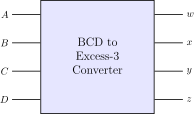
\includegraphics[width=165.5pt]{lect_5_bcd_to_excess3_block}\caption{block diagram}\label{fig:bcd-e3-block}
\end{subfigure}
\\[6pt]
\begin{subfigure}[b]{258.3pt}\centering
  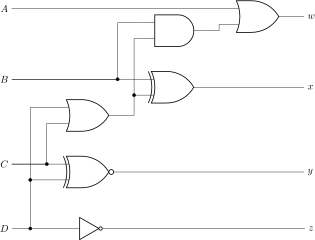
\includegraphics[width=256.3pt]{lect_5_bcd_to_excess3_circuit}\caption{logic diagram}\label{fig:e3-circuit}
\end{subfigure}
\caption{BCD to excess-3 converter of \cref{ex:excess3}.}
\end{figure}

\begin{figure}[htbp]
\centering
\begin{subfigure}[b]{382.0pt}\centering
  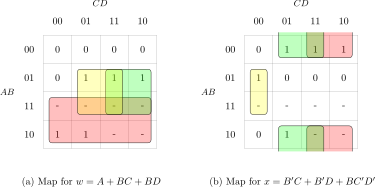
\includegraphics[width=380.0pt]{lect_5_bcd_kmaps_wx}\caption{K-maps for $w$ and $x$}
\end{subfigure}
\\[6pt]
\begin{subfigure}[b]{382.0pt}\centering
  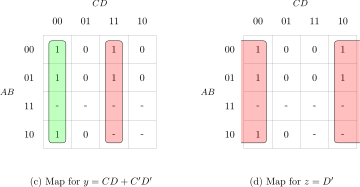
\includegraphics[width=380.0pt]{lect_5_bcd_kmaps_yz}\caption{K-maps for $y$ and $z$}
\end{subfigure}
\caption{K-maps for the outputs of the BCD to excess-3 converter; X marks don't-care inputs.}\label{fig:e3-kmaps}
\end{figure}

\vhdlfile{listings/ch05_bcd_to_excess3.vhd}{VHDL of the BCD to excess-3 converter.}{lst:e3}

\section{Decimal (BCD) Adder}\label{sec:bcdadder}
A \term{BCD adder} adds two BCD digits (plus a carry-in) and produces a BCD sum digit and a carry-out. A direct design would have 8 inputs (plus carry-in), a truth table with 256 rows and no usable K-map. A better idea is to reuse the 4-bit binary adder:
\begin{enumerate}
  \item add the two digits with a binary adder; the sum $Z$ (with carry $K$) lies between 0 and 19 ($9+9+1$);
  \item if the binary sum is 9 or less it is already the correct BCD digit;
  \item if it exceeds 9, add 6 ($\bin{0110}$): the extra 6 skips the six unused codes 10--15 and produces the correct decimal digit and a carry to the next decade.
\end{enumerate}
A correction is therefore needed if $K=1$ (sums 16--19) or if $Z\in\{10,\dots,15\}$ ($K=0$). In the latter range $Z_3=1$ always, and either $Z_2=1$ (12--15) or $Z_1=1$ (10, 11, 14, 15). The correction (and the carry-out) is
\begin{equation}
  C = K + Z_3Z_2 + Z_3Z_1 .
  \label{eq:bcdcorr}
\end{equation}
\Cref{fig:bcd-adder} shows the arrangement: the first adder forms $Z$, the logic of \cref{eq:bcdcorr} detects sums above 9, and the second adder adds $0110$ when $C=1$ and $0000$ otherwise.

\begin{example}{Adding BCD digits}{bcdadd}
$7+5$: the binary sum is $\bin{0111}+\bin{0101}=\bin{1100}=12>9$, so add $\bin{0110}$: $\bin{1100}+\bin{0110}=\bin{1\,0010}$. The carry is 1 and the digit is $\bin{0010}$: the BCD number $\bin{0001\,0010}=12$. \quad
$9+8+1$: $\bin{1001}+\bin{1000}+1=\bin{1\,0010}$, so $K=1$; adding 6 gives $\bin{1\,1000}$, the digit $\bin{1000}=8$ and carry 1, i.e.\ $18$.
\end{example}

\figw{206.8pt}{lect_5_bcd_adder}{A one-digit BCD adder: a binary adder, the correction-detection logic and a second adder that adds 6.}{fig:bcd-adder}

\vhdlfile{listings/ch05_bcd_adder.vhd}{Behavioural VHDL of a one-digit BCD adder. The package \code{numeric_std} provides the type \code{unsigned} and arithmetic on it.}{lst:bcdadder}

\section{Decoders}\label{sec:decoders}
A \term{decoder} converts binary information from $n$ input lines to at most $2^n$ unique output lines, so that for each input combination exactly one output is active. A decoder with $n$ inputs and $m\le2^n$ outputs is called an $n$-to-$m$-line decoder. \Cref{tab:dec38} gives the truth table of a 3-to-8 decoder, which is simply a generator of all eight \emph{minterms} of the three inputs: output $D_i$ is the minterm $m_i$. \Cref{fig:dec38} shows the block and its AND-gate implementation, and \cref{lst:dec} the VHDL.

\begin{table}[htbp]
\centering
\small
\caption{Truth table of a 3-to-8-line decoder (active-high outputs).}
\label{tab:dec38}
\begin{tabular}{ccc|cccccccc}
\toprule
$x$&$y$&$z$&$D_0$&$D_1$&$D_2$&$D_3$&$D_4$&$D_5$&$D_6$&$D_7$\\ \midrule
0&0&0&\textbf{1}&0&0&0&0&0&0&0\\
0&0&1&0&\textbf{1}&0&0&0&0&0&0\\
0&1&0&0&0&\textbf{1}&0&0&0&0&0\\
0&1&1&0&0&0&\textbf{1}&0&0&0&0\\
1&0&0&0&0&0&0&\textbf{1}&0&0&0\\
1&0&1&0&0&0&0&0&\textbf{1}&0&0\\
1&1&0&0&0&0&0&0&0&\textbf{1}&0\\
1&1&1&0&0&0&0&0&0&0&\textbf{1}\\ \bottomrule
\end{tabular}
\end{table}

\begin{figure}[htbp]
\centering
\begin{subfigure}[b]{169.5pt}\centering
  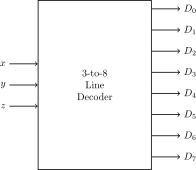
\includegraphics[width=167.5pt]{lect_5_decoder_3to8_block}\caption{block diagram}
\end{subfigure}
\hfill
\begin{subfigure}[b]{236.3pt}\centering
  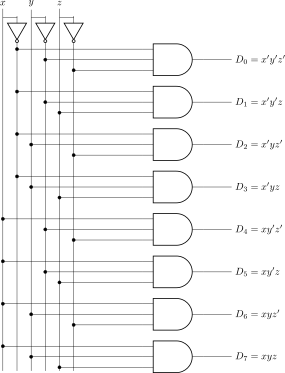
\includegraphics[width=234.3pt]{lect_5_decoder_3to8_circuit}\caption{logic diagram}
\end{subfigure}
\caption{A 3-to-8-line decoder.}\label{fig:dec38}
\end{figure}

\vhdlfile{listings/ch05_decoder_3to8.vhd}{A 3-to-8 decoder in VHDL.}{lst:dec}

\paragraph{Decoder with enable.} Decoders usually have an \term{enable} input $E$. In the common NAND-gate implementation of \cref{tab:dec-en} the outputs are active-low and the decoder works when $E=0$; when $E=1$ all outputs are inactive (1). \Cref{fig:dec-en} shows the circuit. Enable inputs allow decoders to be \emph{cascaded}: two 3-to-8 decoders form a 4-to-16 decoder if the most significant input drives the enable of one decoder directly and of the other through an inverter (\cref{fig:dec416}).

\begin{table}[htbp]
\centering
\scriptsize
\caption{3-to-8 decoder with active-low enable $E$ and active-low outputs.}
\label{tab:dec-en}
\begin{tabular}{c|ccc|cccccccc}
\toprule
$E$&$x$&$y$&$z$&$D_0$&$D_1$&$D_2$&$D_3$&$D_4$&$D_5$&$D_6$&$D_7$\\ \midrule
1&X&X&X&1&1&1&1&1&1&1&1\\
0&0&0&0&\textbf{0}&1&1&1&1&1&1&1\\
0&0&0&1&1&\textbf{0}&1&1&1&1&1&1\\
0&0&1&0&1&1&\textbf{0}&1&1&1&1&1\\
0&0&1&1&1&1&1&\textbf{0}&1&1&1&1\\
0&1&0&0&1&1&1&1&\textbf{0}&1&1&1\\
0&1&0&1&1&1&1&1&1&\textbf{0}&1&1\\
0&1&1&0&1&1&1&1&1&1&\textbf{0}&1\\
0&1&1&1&1&1&1&1&1&1&1&\textbf{0}\\ \bottomrule
\end{tabular}
\end{table}

\begin{figure}[htbp]
\centering
\begin{subfigure}[b]{229.3pt}\centering
  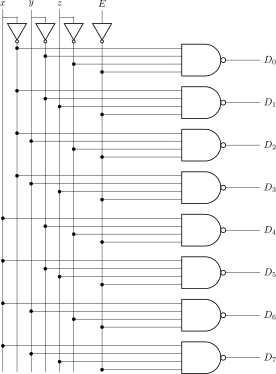
\includegraphics[width=227.3pt]{lect_5_decoder_3to8_enable_circuit}\caption{3-to-8 decoder with enable}\label{fig:dec-en}
\end{subfigure}
\caption{Decoder with enable input and cascading.}
\end{figure}

\begin{figure}[htbp]
\centering
\ContinuedFloat
\begin{subfigure}[b]{186.7pt}\centering
  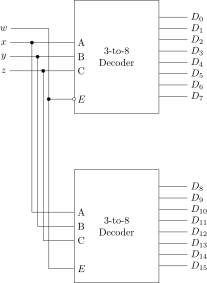
\includegraphics[width=184.7pt]{lect_5_decoder_4to16_block}\caption{4-to-16 decoder from two 3-to-8 decoders}\label{fig:dec416}
\end{subfigure}
\caption[]{Decoder with enable input and cascading.}
\end{figure}

\begin{keypoint}[Decoders implement functions]
Because the outputs of a decoder are the minterms of its inputs, any combinational function of $n$ variables can be implemented by an $n$-to-$2^n$ decoder and an OR gate that collects the minterms for which $f=1$. For example the full adder is $S=\Sm(1,2,4,7)$ and $C_{out}=\Sm(3,5,6,7)$: one 3-to-8 decoder and two 4-input OR gates.
\end{keypoint}

\subsection{Demultiplexers}
A \term{demultiplexer} (DEMUX) does the opposite of a multiplexer: it takes data from a single input line and routes it to one of $2^n$ output lines selected by $n$ select lines. A decoder with an enable input is a demultiplexer: the \emph{enable} becomes the \emph{data input} and the decoder inputs become the select inputs. \Cref{tab:demux} and \cref{fig:demux} show a 1-to-4 demultiplexer.

\begin{table}[htbp]
\centering
\caption{1-to-4 demultiplexer.}
\label{tab:demux}
\begin{tabular}{c|cc|cccc}
\toprule
Data&$S_1$&$S_0$&$Y_0$&$Y_1$&$Y_2$&$Y_3$\\ \midrule
$D$&0&0&$D$&0&0&0\\ $D$&0&1&0&$D$&0&0\\ $D$&1&0&0&0&$D$&0\\ $D$&1&1&0&0&0&$D$\\ \bottomrule
\end{tabular}
\end{table}

\figw{317.8pt}{lect_5_demux_1to4}{A 1-to-4 demultiplexer.}{fig:demux}

\section{Encoders}\label{sec:encoders}
An \term{encoder} performs the inverse of a decoder: it has $2^n$ (or fewer) input lines and $n$ output lines, and produces the binary code of the input line that is active. It is assumed that only one input is active at a time. For the octal-to-binary encoder with inputs $D_0,\dots,D_7$ and outputs $xyz$ (\cref{fig:enc83}),
\[
 x = D_4+D_5+D_6+D_7,\qquad y = D_2+D_3+D_6+D_7,\qquad z = D_1+D_3+D_5+D_7 .
\]
Each output is the OR of the inputs whose code has a 1 in that bit position. The simple encoder has two defects: the output is undefined if more than one input is active, and the all-zero output code is produced both by $D_0$ and by no input at all.

\figw{267.2pt}{lect_5_encoder_8to3_circuit}{An octal-to-binary (8-to-3) encoder.}{fig:enc83}

\subsection{Priority encoders}
A \term{priority encoder} gives each input a priority and outputs the code of the active input with the \emph{highest priority}. It also has a \emph{valid} output $V$ that shows whether any input is active, which resolves the second defect. \Cref{tab:prio} is the truth table of a 4-input priority encoder in which $D_3$ has the highest priority; X means don't-care. From it,
\[
 x = D_3 + D_2,\qquad y = D_3 + D_2'D_1,\qquad V = D_3+D_2+D_1+D_0 ,
\]
and \cref{fig:prio} is the circuit. Priority encoders are used, for example, to arbitrate interrupt requests.

\begin{table}[htbp]
\centering
\caption{4-to-2 priority encoder ($D_3$ has the highest priority).}
\label{tab:prio}
\begin{tabular}{cccc|ccc}
\toprule
$D_3$&$D_2$&$D_1$&$D_0$&$x$&$y$&$V$\\ \midrule
0&0&0&0&X&X&0\\0&0&0&1&0&0&1\\0&0&1&X&0&1&1\\0&1&X&X&1&0&1\\1&X&X&X&1&1&1\\ \bottomrule
\end{tabular}
\end{table}

\figw{237.0pt}{lect_5_priority_encoder_circuit}{A 4-to-2 priority encoder.}{fig:prio}

\section{Multiplexers}\label{sec:mux}
A \term{multiplexer} (MUX, or data selector) selects one of $2^n$ data inputs and connects it to a single output; $n$ \emph{select} lines determine which. We met the 2-to-1 multiplexer in \cref{ex:mux}. For the 4-to-1 multiplexer (\cref{tab:mux4}, \cref{fig:mux4}),
\[
 Y = S_1'S_0'I_0 + S_1'S_0I_1 + S_1S_0'I_2 + S_1S_0I_3 .
\]
\Cref{lst:mux-b} describes it behaviourally, as a selection (\code{when ... else}); \cref{lst:mux-s} gives the same function as a Boolean expression. Both produce the same hardware after synthesis, but the behavioural style is shorter and much easier to read and to scale to wider multiplexers.

\begin{table}[htbp]
\centering
\caption{4-to-1 multiplexer.}
\label{tab:mux4}
\begin{tabular}{cc|c}
\toprule $S_1$&$S_0$&$Y$\\ \midrule 0&0&$I_0$\\0&1&$I_1$\\1&0&$I_2$\\1&1&$I_3$\\ \bottomrule
\end{tabular}
\end{table}

\figw{262.8pt}{lect_5_mux_4to1_logic}{Logic diagram of a 4-to-1 multiplexer.}{fig:mux4}

\vhdlfile{listings/ch05_mux_4to1_behav.vhd}{4-to-1 multiplexer, behavioural architecture.}{lst:mux-b}
\vhdlfile{listings/ch05_mux_4to1_struct.vhd}{4-to-1 multiplexer written as a Boolean expression (``structural'' in the lecture notes).}{lst:mux-s}

\subsection{Implementing Boolean functions with multiplexers}
A multiplexer is a \emph{universal logic module}: any Boolean function of $n$ variables can be implemented by a multiplexer with $n-1$ select lines.
\begin{enumerate}
  \item Connect $n-1$ of the variables to the select inputs.
  \item Using an \emph{implementation table}, express $F$ for each select combination as a function of the remaining variable $D$. It is always one of $D$, $D'$, $0$ or $1$.
  \item Connect each data input $I_k$ to the corresponding $D$, $D'$, 0 or 1.
\end{enumerate}

\begin{example}{Function with an 8-to-1 multiplexer}{muxfunc}
Implement $F(A,B,C,D)=\Sm(1,3,4,11,12,13,14,15)$ with an 8-to-1 multiplexer.

\textbf{Solution.} Connect $A,B,C$ to the select inputs $S_2,S_1,S_0$. For each $ABC$ pair of rows, see where $F=1$ (\cref{tab:muximpl}). The data inputs are
\[
 I_0=D,\ I_1=D,\ I_2=D',\ I_3=0,\ I_4=0,\ I_5=D,\ I_6=1,\ I_7=1 .
\]
The circuit is \cref{fig:mux8}.
\end{example}

\begin{table}[htbp]
\centering
\small
\caption{Implementation table for \cref{ex:muxfunc}.}
\label{tab:muximpl}
\begin{tabular}{ccc|cc|c}
\toprule
$A$&$B$&$C$&$F$ for $D=0$&$F$ for $D=1$&Data input\\ \midrule
0&0&0&0&1&$I_0=D$\\
0&0&1&0&1&$I_1=D$\\
0&1&0&1&0&$I_2=D'$\\
0&1&1&0&0&$I_3=0$\\
1&0&0&0&0&$I_4=0$\\
1&0&1&0&1&$I_5=D$\\
1&1&0&1&1&$I_6=1$\\
1&1&1&1&1&$I_7=1$\\ \bottomrule
\end{tabular}
\end{table}

\figw{202.2pt}{lect_5_mux_8to1_func}{\Cref{ex:muxfunc}: a four-variable function with an 8-to-1 multiplexer.}{fig:mux8}

\subsection{Shannon's expansion theorem}
\term{Shannon's expansion theorem} states that any Boolean function can be split about any variable $x_i$:
\begin{equation}
  F(x_1,\dots,x_n) = x_i'\,F(x_1,\dots,0,\dots,x_n) + x_i\,F(x_1,\dots,1,\dots,x_n).
  \label{eq:shannon}
\end{equation}
The two terms are the \emph{cofactors} of $F$ with respect to $x_i$. Equation~\eqref{eq:shannon} is exactly the equation of a 2-to-1 multiplexer with select input $x_i$ and data inputs the two cofactors. Repeating the expansion for further variables gives a tree of 2-to-1 multiplexers: any $n$-variable function can be built from at most $2^{n-1}-1$ of them, with the last variable (or a constant) at the leaves.

\begin{example}{Multiplexer tree}{shannon}
Implement $F(A,B,C)=AB+C$ with 2-to-1 multiplexers.

\textbf{Solution.} Expanding on $A$: $F_{A'}=C$ and $F_A=B+C$. Expanding $F_A$ on $B$: $F_{AB'}=C$ and $F_{AB}=1$. Hence one multiplexer selected by $B$ with inputs $(C,1)$ produces $F_A$, and a second one selected by $A$ with inputs $(C, F_A)$ produces $F$ (\cref{fig:mux-tree}); two multiplexers suffice.
\end{example}

\figw{188.9pt}{lect_5_mux_tree_3var}{Multiplexer tree for a function of three variables.}{fig:mux-tree}

\section{The Arithmetic Logic Unit}\label{sec:alu}
An \term{arithmetic logic unit} (ALU) is a combinational circuit that performs a set of arithmetic and logic operations on two binary operands, the operation being chosen by select inputs. It is the computational core of every processor. A classic example is the 4-bit 74381 ALU (\cref{fig:alu-block}), which performs the eight operations of \cref{tab:alu} on operands $A$ and $B$ under the control of three inputs $S_2S_1S_0$. It also produces \emph{group propagate} and \emph{group generate} outputs, which serve as the inputs $P^*$ and $G^*$ of a carry-lookahead generator (\cref{sec:cla}), so that wider ALUs can be built without a long carry delay.

\begin{table}[htbp]
\centering
\caption{Function table of the 74381 ALU.}
\label{tab:alu}
\begin{tabular}{ccc|ll}
\toprule
$S_2$&$S_1$&$S_0$&Function&Operation\\ \midrule
0&0&0&Clear&$F=0000$\\
0&0&1&Subtract&$F=B-A$\\
0&1&0&Subtract&$F=A-B$\\
0&1&1&Add&$F=A+B$\\
1&0&0&XOR&$F=A\xor B$\\
1&0&1&OR&$F=A+B$ (logical)\\
1&1&0&AND&$F=A\cdot B$\\
1&1&1&Preset&$F=1111$\\ \bottomrule
\end{tabular}
\end{table}

Subtraction uses two's complement ($A+\NOT{B}+1$, \cref{sec:adders}). Each bit slice (\cref{fig:alu-slice}) contains a logic unit (AND, OR, XOR), an arithmetic unit (a full adder in propagate/generate form, $P_i=A_i\xor B_i$, $G_i=A_iB_i$) and a multiplexer, controlled by the select inputs, that chooses the result of the slice.

\begin{figure}[htbp]
\centering
\begin{subfigure}[b]{227.6pt}\centering
  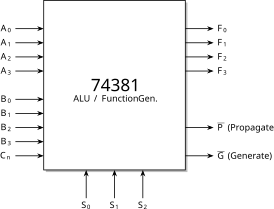
\includegraphics[width=225.6pt]{lect_5_alu_74381_block}\caption{block symbol}\label{fig:alu-block}
\end{subfigure}
\caption{The 74381 ALU: symbol and one bit slice.}
\end{figure}

\begin{figure}[htbp]
\centering
\ContinuedFloat
\begin{subfigure}[b]{412.0pt}\centering
  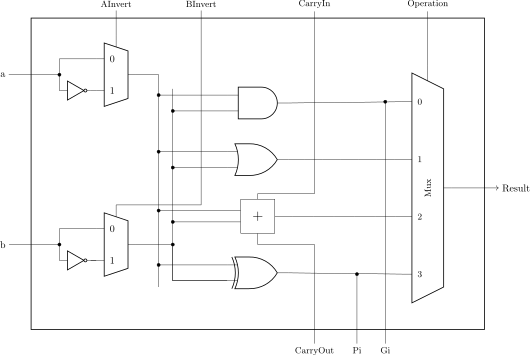
\includegraphics[width=410.0pt]{lect_5_alu_74381_logic}\caption{simplified 1-bit slice}\label{fig:alu-slice}
\end{subfigure}
\caption[]{The 74381 ALU: symbol and one bit slice.}
\end{figure}

\section{Three-State Gates and Buses}\label{sec:tristate}
A \term{three-state gate} (tri-state buffer) has three output states: logic 0, logic 1 and \term{high impedance} (Hi-Z), in which the output is effectively disconnected, like an open circuit. A control input $C$ selects the state: if $C=1$ the buffer is enabled and $\mathrm{Output}=\mathrm{Input}$; if $C=0$ the output is Hi-Z (\cref{fig:tristate}).

Three-state gates make it possible to connect several devices to a common wire, a \term{bus}, so long as \emph{only one device drives the bus at a time}. Two ordinary gates cannot drive the same wire: if one outputs 1 and the other 0 there is a low-resistance path between the supply and ground through the two output stages, a condition called \emph{bus contention} that causes a large current and an undefined voltage. \Cref{lst:tristate} shows the buffer in VHDL; the value \code{'Z'} of \code{std_logic} stands for high impedance. A three-state output can only be described behaviourally, because high impedance is a property of the output driver and cannot be formed from AND/OR/NOT gates.

\figw{147.7pt}{lect_5_tri_state_buffer}{A three-state buffer with enable input $C$.}{fig:tristate}

\vhdlfile{listings/ch05_tri_state_buffer.vhd}{A three-state buffer.}{lst:tristate}

\section{Magnitude Comparator}\label{sec:comparator}
A \term{magnitude comparator} compares two binary numbers $A$ and $B$ and produces three outputs: $A>B$, $A=B$ and $A<B$. The comparison proceeds from the most significant bit. Let $x_i = A_i\odot B_i = (A_i\xor B_i)'$ be 1 when the bits at position $i$ are equal. Then, for 4-bit numbers,
\begin{align*}
 (A=B) &= x_3x_2x_1x_0,\\
 (A>B) &= A_3B_3' + x_3A_2B_2' + x_3x_2A_1B_1' + x_3x_2x_1A_0B_0',\\
 (A<B) &= A_3'B_3 + x_3A_2'B_2 + x_3x_2A_1'B_1 + x_3x_2x_1A_0'B_0 .
\end{align*}
$A>B$ if at some position $A_i=1$, $B_i=0$ and all more significant bits are equal. The circuit is \cref{fig:comparator}; \cref{lst:comp-b,lst:comp-s} describe it behaviourally, and structurally with the equations above.

\figw{410.0pt}{lect_5_magnitude_comparator}{A 4-bit magnitude comparator.}{fig:comparator}

\vhdlfile{listings/ch05_magnitude_comparator_behav.vhd}{Behavioural description of the comparator using the relational operators.}{lst:comp-b}
\vhdlfile{listings/ch05_magnitude_comparator_struct.vhd}{Gate-level description of the comparator.}{lst:comp-s}

\begin{chaptersummary}
\begin{itemize}
  \item A \textbf{combinational circuit} has no memory. \textbf{Analysis}: label gate outputs, derive functions, build the truth table, explain. \textbf{Design}: specification, truth table, simplification, logic diagram, verification.
  \item \textbf{Code converters} such as BCD to excess-3 are designed with K-maps and don't-cares. The \textbf{BCD adder} adds 6 to a binary sum greater than 9, with $C=K+Z_3Z_2+Z_3Z_1$.
  \item A \textbf{decoder} generates the minterms of its inputs; with an enable input it is also a \textbf{demultiplexer} and can be cascaded. Any function can be built from a decoder and an OR gate.
  \item An \textbf{encoder} produces the code of the active input; a \textbf{priority encoder} handles several active inputs and has a valid output.
  \item A \textbf{multiplexer} selects one of $2^n$ inputs; it implements any function of $n+1$ variables, and Shannon's expansion gives a tree of 2-to-1 multiplexers.
  \item An \textbf{ALU} selects among arithmetic and logic operations; its group $P$ and $G$ outputs permit fast wide ALUs.
  \item \textbf{Three-state gates} (Hi-Z) allow many drivers on one bus, provided only one is enabled at a time.
  \item A \textbf{magnitude comparator} compares from the MSB downward using $x_i=A_i\odot B_i$.
\end{itemize}
\end{chaptersummary}

\chapsec{Exercises}
\begin{exlist}
  \item \textbf{Multiplexer expansion.} Construct a 4-to-1 multiplexer using only 2-to-1 multiplexers. How many are needed? \emph{Hint:} use the LSB select line $S_0$ in the first stage to choose within the pairs $(I_0,I_1)$ and $(I_2,I_3)$, and the MSB $S_1$ in the second stage.
  \item \textbf{Function with a 4-to-1 multiplexer.} Implement $F(A,B,C)=\Sm(1,3,5,6,7)$ with a single 4-to-1 multiplexer. Connect $A$ and $B$ to the select lines and find $I_0,\dots,I_3$ in terms of $C$.
  \item \textbf{Tri-state bus.} Explain why the outputs of two ordinary AND gates cannot be connected together to the same wire. What happens if one gate outputs 1 and the other 0? How does a three-state buffer solve the problem?
  \item \textbf{Comparator analysis.} For $A=\bin{1011}$ and $B=\bin{1001}$, find the equivalence signals $x_3,x_2,x_1,x_0$ and the outputs $A>B$, $A=B$, $A<B$.
  \item Analyse the circuit defined by $T_1=AB'$, $T_2=A'B$, $F=T_1+T_2+C$. Write $F$ as a function of $A,B,C$, make the truth table and describe the function in words.
  \item Implement the full adder ($S$ and $C_{out}$) with a 3-to-8 decoder (active-high outputs) and OR gates.
  \item Design a 4-to-2 priority encoder in which $D_0$ has the \emph{highest} priority and $D_3$ the lowest. Give the equations for $x$, $y$ and $V$.
  \item Implement $F(A,B,C,D)=\Sm(0,2,6,7,8,10,13,15)$ with an 8-to-1 multiplexer, using $A,B,C$ as the select inputs. Give the data inputs in terms of $D$.
  \item Implement $F=xy+x'z$ with a single 2-to-1 multiplexer. Identify the select and data inputs.
  \item Show how to build a 5-to-32 decoder from 3-to-8 decoders with enable inputs and one 2-to-4 decoder. How many of each are needed?
  \item How many 2-to-1 multiplexers are needed to build an 8-to-1 multiplexer?
  \item Add the BCD digits (a)~$\bin{0111}+\bin{0101}$ and (b)~$\bin{1001}+\bin{1001}+1$ using the BCD adder method, giving the binary sum, the correction and the result.
  \item Design a 2-bit magnitude comparator with outputs $A>B$, $A=B$, $A<B$ and draw the logic diagram. \emph{Hint:} $A>B = A_1B_1' + (A_1\odot B_1)A_0B_0'$.
  \item Design a combinational circuit that converts a 4-bit \emph{binary} number in the range 0--9 into the corresponding Gray code of that number, ($g_3=b_3$, $g_2=b_3\xor b_2$, $g_1=b_2\xor b_1$, $g_0=b_1\xor b_0$). Write its VHDL in one architecture with four concurrent assignments.
  \item A three-state buffer drives the bus with the value of an 8-bit register when the signal \code{rd} is 1. Write the VHDL, using a \code{std_logic_vector} of width 8 and the value \code{(others => 'Z')}.
\end{exlist}

\chapsec{Further Reading}
All the blocks of this chapter are treated in Chapter~4 of Mano and Ciletti~\cite{mano2018} and in Chapters~6 and~7 of Brown and Vranesic~\cite{brown2009}, including the VHDL descriptions; Wakerly~\cite{wakerly2006} also discusses MSI parts in detail. Ashenden~\cite{ashenden2008} is a good reference for the VHDL features used in the listings.

\chapter{Latches, Flip-Flops and Synchronous Sequential Circuits}\label{ch:latches}

\begin{objectives}
After studying this chapter you will be able to:
\begin{itemize}
  \item explain why a digital system needs memory and describe the general structure of a sequential circuit;
  \item distinguish synchronous from asynchronous circuits, and level-triggered latches from edge-triggered flip-flops;
  \item describe the operation of the SR, $\overline{S}\overline{R}$, gated SR and D latches, and of the D, JK and T flip-flops, using characteristic tables and equations;
  \item write VHDL for latches and flip-flops, with synchronous and asynchronous reset;
  \item analyse a clocked sequential circuit by deriving its state table and state diagram;
  \item distinguish the Mealy and Moore models; and
  \item design a synchronous sequential circuit with D, JK and T flip-flops using excitation tables.
\end{itemize}
\end{objectives}

\section{Why Sequential Circuits?}
The combinational circuits of Chapters~2--5 have one limitation: their output depends \emph{only} on the present input, and they have no memory of the past. Many real systems need such a memory:
\begin{itemize}
  \item a \textbf{vending machine} must know how much money \emph{has been} inserted;
  \item a \textbf{combination lock} must know whether the \emph{previous} digits were correct;
  \item a \textbf{counter} must know its \emph{present} value to compute the next.
\end{itemize}
The information that must be remembered is called the \term{state} of the system, and circuits that store it are built from \emph{memory elements}: latches and flip-flops.

\section{Structure of a Sequential Circuit}
A \term{sequential circuit} (\cref{fig:seq-block}) consists of a combinational circuit and memory elements connected in a loop. The memory elements hold the \emph{present state}; the combinational logic computes the \emph{next state} and the \emph{outputs} from the inputs and the present state; and the next state is stored in the memory elements at the next clock pulse. The feedback loop through the memory is what distinguishes a sequential from a combinational circuit.

\figside{472.2pt}{lect_6_sequential_circuit_block}{Block diagram of a sequential circuit: combinational logic, memory elements and the state feedback.}{fig:seq-block}

Sequential circuits are of two kinds.
\begin{itemize}
  \item In a \term{synchronous} sequential circuit state changes happen only at discrete instants, determined by a periodic signal called the \term{clock}. The memory elements are \emph{flip-flops}. Synchronous design is the dominant style because it is easier to design and verify and avoids many timing problems.
  \item In an \term{asynchronous} sequential circuit the state may change whenever an input changes. The memory elements are often simple \emph{latches}. Asynchronous circuits are faster but difficult to design reliably, and are outside the scope of this book.
\end{itemize}

\section{Latches}\label{sec:latches}
A \term{latch} is the simplest memory element: a circuit with two stable states, a \emph{bistable} circuit, that can store one bit as long as power is applied.

\subsection{The SR latch}
The \term{SR latch} (\cref{fig:sr-nor}) consists of two cross-coupled NOR gates; the inputs are \emph{Set} ($S$) and \emph{Reset} ($R$). Its behaviour (\cref{tab:sr-nor}) is:
\begin{itemize}
  \item $S=R=0$: no change; the latch remembers its state;
  \item $S=1,R=0$: \emph{set}: $Q=1$;
  \item $S=0,R=1$: \emph{reset}: $Q=0$;
  \item $S=R=1$: \emph{forbidden}: both outputs go to 0, violating $Q'=\overline{Q}$, and when both inputs return to 0 simultaneously the final state is unpredictable. This input combination must be avoided.
\end{itemize}
The memory comes from the feedback: when $S=R=0$ each gate acts as an inverter, and the two inverters in a loop hold whatever state they have.

\begin{table}[htbp]
\centering
\caption{SR latch with NOR gates.}
\label{tab:sr-nor}
\begin{tabular}{cc|cc|l}
\toprule
$S$&$R$&$Q(t+1)$&$Q'(t+1)$&State\\ \midrule
0&0&$Q$&$Q'$&no change\\0&1&0&1&reset\\1&0&1&0&set\\1&1&0&0&invalid\\ \bottomrule
\end{tabular}
\end{table}

\subsection{The $\overline{S}\overline{R}$ latch}
With NAND gates the same circuit has \emph{active-low} inputs, $\overline{S}$ and $\overline{R}$ (\cref{fig:sr-nand}, \cref{tab:sr-nand}): $(\overline{S},\overline{R})=(1,1)$ holds the state, $(0,1)$ sets, $(1,0)$ resets, and $(0,0)$ is invalid (both outputs 1).

\begin{table}[htbp]
\centering
\caption{$\overline{S}\overline{R}$ latch with NAND gates.}
\label{tab:sr-nand}
\begin{tabular}{cc|cc|l}
\toprule
$\overline{S}$&$\overline{R}$&$Q(t+1)$&$Q'(t+1)$&State\\ \midrule
0&0&1&1&invalid\\0&1&1&0&set\\1&0&0&1&reset\\1&1&$Q$&$Q'$&no change\\ \bottomrule
\end{tabular}
\end{table}

\begin{figure}[htbp]
\centering
\begin{subfigure}[b]{129.4pt}\centering
  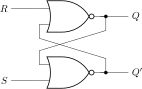
\includegraphics[width=127.4pt]{lect_6_sr_latch_nor}\caption{NOR SR latch}\label{fig:sr-nor}
\end{subfigure}
\hfill
\begin{subfigure}[b]{129.4pt}\centering
  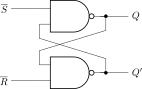
\includegraphics[width=127.4pt]{lect_6_sr_latch_nand}\caption{NAND $\overline{S}\overline{R}$ latch}\label{fig:sr-nand}
\end{subfigure}
\caption{Basic latches built from cross-coupled gates.}
\end{figure}

\subsection{Gated SR latch and D latch}
Adding two gates and a control input $C$ makes the latch respond to $S$ and $R$ only while $C=1$ (\cref{fig:gated}a): when $C=0$ the latch holds its state. This is the \term{gated SR latch}. To remove the forbidden input combination, an inverter ensures that $S$ and $R$ are never 1 together: connect $S=D$ and $R=D'$. The result is the \term{D latch} (\cref{fig:gated}b, \cref{tab:dlatch}): while $C=1$, $Q$ follows $D$ (the latch is \emph{transparent}); when $C=0$ the latch holds the last value of $D$. Its equation is $Q(t+1)=D$ when $C=1$.

\begin{table}[htbp]
\centering
\caption{D latch.}
\label{tab:dlatch}
\begin{tabular}{cc|l}
\toprule $C$&$D$&$Q(t+1)$\\ \midrule 0&X&no change\\1&0&0 (reset)\\1&1&1 (set)\\ \bottomrule \end{tabular}
\end{table}

\begin{figure}[htbp]
\centering
\begin{subfigure}[b]{207.4pt}\centering
  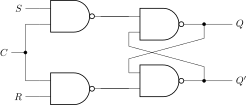
\includegraphics[width=205.4pt]{lect_6_gated_sr_latch}\caption{gated SR latch}
\end{subfigure}
\\[6pt]
\begin{subfigure}[b]{250.5pt}\centering
  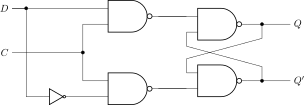
\includegraphics[width=248.5pt]{lect_6_d_latch}\caption{D latch}
\end{subfigure}
\caption{Gated latches.}\label{fig:gated}
\end{figure}

\figw{292.1pt}{lect_6_latch_symbols}{Graphical symbols of the SR, $\overline{S}\overline{R}$ and D latches.}{fig:latch-symbols}

\vhdlfile{listings/ch06_d_latch.vhd}{A D latch. The process is sensitive to both \code{D} and \code{C}; since no value is assigned when \code{C} is 0, the synthesis tool infers a latch.}{lst:dlatch}

\Cref{lst:dlatch} shows how a latch is described: the process has no \code{else} branch, so \code{Q} keeps its value when \code{C = '0'}, which means memory. Unintentional latches caused by incomplete \code{if} statements are a common mistake in combinational VHDL descriptions.

\section{Flip-Flops}\label{sec:flipflops}
A latch is \term{level-triggered}: its output may change at any time while the control input is active. In a circuit in which the latch output feeds back into its own input through combinational logic this causes uncontrolled multiple transitions during one clock pulse. A \term{flip-flop} is \term{edge-triggered}: it samples its inputs and changes state only at one \emph{edge} of the clock (\cref{fig:trigger}), so that all state changes in a synchronous system happen at the same moment. In a \emph{positive-edge} flip-flop the transition is on the rising edge (0 $\to$ 1), in a \emph{negative-edge} flip-flop on the falling edge (1 $\to$ 0).

\figw{191.7pt}{lect_6_trigger_types}{Level triggering, positive-edge triggering and negative-edge triggering.}{fig:trigger}

\subsection{The D flip-flop}
The D flip-flop is the most common flip-flop. At the active clock edge it captures the value of $D$ and stores it in $Q$. One way to build it is the \emph{master--slave} configuration of \cref{fig:ms}: two D latches in series with opposite clock polarity. While CLK is 1 the master latch is transparent and follows $D$ while the slave is closed and holds the old value. When CLK falls to 0 the master closes, capturing $D$, and the slave opens and passes the captured value to $Q$. $Q$ therefore changes only when the clock falls: a negative-edge D flip-flop. The characteristic equation is $Q(t+1)=D$.

\begin{figure}[htbp]
\centering
\begin{subfigure}[b]{208.9pt}\centering
  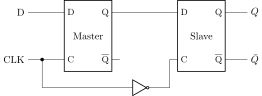
\includegraphics[width=206.9pt]{lect_6_master_slave_d_flip_flop}\caption{master--slave construction}
\end{subfigure}
\hfill
\begin{subfigure}[b]{145.3pt}\centering
  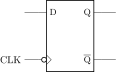
\includegraphics[width=143.3pt]{lect_6_d_flip_flop_neg_edge}\caption{symbols}
\end{subfigure}
\caption{Edge-triggered D flip-flop.}\label{fig:ms}
\end{figure}

\subsection{The JK flip-flop}
The \term{JK flip-flop} refines the SR flip-flop by giving meaning to the forbidden input. $J$ sets, $K$ resets, and when $J=K=1$ the flip-flop \emph{toggles}: $Q$ becomes $Q'$. Its characteristic equation is
\[
 Q(t+1) = JQ' + K'Q .
\]
A JK flip-flop can be built from a D flip-flop with the input equation $D=JQ'+K'Q$ (\cref{fig:jk}).

\subsection{The T flip-flop}
The \term{T flip-flop} has a single input $T$: if $T=0$ it holds its state and if $T=1$ it toggles, $Q(t+1)=T\xor Q$. It is useful for counters. It is obtained from a JK flip-flop by tying $J=K=T$, or from a D flip-flop with an XOR gate, $D=T\xor Q$ (\cref{fig:tff}).

\begin{figure}[htbp]
\centering
\begin{subfigure}[b]{304.6pt}\centering
  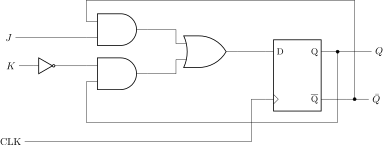
\includegraphics[width=302.6pt]{lect_6_jk_flip_flop_from_d}\caption{JK from a D flip-flop}
\end{subfigure}
\\[6pt]
\begin{subfigure}[b]{145.3pt}\centering
  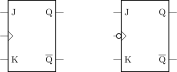
\includegraphics[width=143.3pt]{lect_6_jk_flip_flop_symbol}\caption{JK symbol}
\end{subfigure}
\caption{JK flip-flop.}\label{fig:jk}
\end{figure}

\begin{figure}[htbp]
\centering
\begin{subfigure}[b]{145.3pt}\centering
  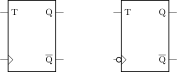
\includegraphics[width=143.3pt]{lect_6_t_flip_flop_symbol}\caption{symbol}
\end{subfigure}
\hfill
\begin{subfigure}[b]{124.0pt}\centering
  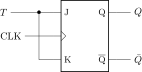
\includegraphics[width=122.0pt]{lect_6_t_flip_flop_from_jk}\caption{from JK}
\end{subfigure}
\\[6pt]
\begin{subfigure}[b]{180.6pt}\centering
  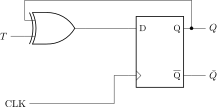
\includegraphics[width=178.6pt]{lect_6_t_flip_flop_from_d}\caption{from D and XOR}
\end{subfigure}
\caption{T flip-flop.}\label{fig:tff}
\end{figure}

\subsection{Characteristic tables}
The behaviour of each flip-flop is summarised by its \term{characteristic table}, which gives the next state $Q(t+1)$ as a function of the inputs and the present state $Q(t)$, and by the equivalent \term{characteristic equation} (\cref{tab:char}). The SR equation $Q(t+1)=S+R'Q$ holds under the restriction $SR=0$.

\begin{table}[htbp]
\centering
\caption{Characteristic tables and equations of the flip-flops.}
\label{tab:char}
\begin{tabular}{@{}cccc@{}}
\toprule
\textbf{SR} & \textbf{D} & \textbf{JK} & \textbf{T}\\ \midrule
$Q(t{+}1)=S+R'Q$ & $Q(t{+}1)=D$ & $Q(t{+}1)=JQ'+K'Q$ & $Q(t{+}1)=T\xor Q$\\[4pt]
\begin{tabular}{cc|c}$S$&$R$&$Q(t{+}1)$\\\hline0&0&$Q$\\0&1&0\\1&0&1\\1&1&?\end{tabular}&
\begin{tabular}{c|c}$D$&$Q(t{+}1)$\\\hline0&0\\1&1\end{tabular}&
\begin{tabular}{cc|c}$J$&$K$&$Q(t{+}1)$\\\hline0&0&$Q$\\0&1&0\\1&0&1\\1&1&$Q'$\end{tabular}&
\begin{tabular}{c|c}$T$&$Q(t{+}1)$\\\hline0&$Q$\\1&$Q'$\end{tabular}\\
\bottomrule
\end{tabular}
\end{table}

\subsection{VHDL descriptions}
In VHDL a flip-flop is described by a process that is sensitive to the clock and does something only at the active edge, detected with the function \code{rising_edge(CLK)} (or \code{falling_edge}). The assignments made in such a process are \emph{registered}: the synthesis tool creates flip-flops. \Cref{lst:dff,lst:jkff,lst:tff} show the D, JK and T flip-flops.

\vhdlfile{listings/ch06_d_ff.vhd}{A positive-edge-triggered D flip-flop.}{lst:dff}
\vhdlfile{listings/ch06_jk_ff.vhd}{A JK flip-flop. The internal signal \code{q_int} lets the value of \code{Q} be read back for the toggle operation.}{lst:jkff}
\vhdlfile{listings/ch06_t_ff.vhd}{A T flip-flop.}{lst:tff}

\subsection{Asynchronous and synchronous reset}
Flip-flops often have \emph{preset} (set $Q=1$) and \emph{clear} or \emph{reset} (set $Q=0$) inputs, shown with a bubble if active-low (\cref{fig:ffpr}). A reset can act in two ways.
\begin{itemize}
  \item An \term{asynchronous} reset overrides the clock and the data input: the output changes \emph{immediately} when the reset becomes active. In VHDL the reset is tested \emph{before} the clock-edge condition (\cref{lst:async}).
  \item A \term{synchronous} reset takes effect only at the active clock edge. In VHDL the reset is tested \emph{inside} the clock-edge condition (\cref{lst:sync}).
\end{itemize}
Asynchronous reset is convenient for initialising a system at power-up; synchronous reset keeps all state changes aligned with the clock. Releasing an asynchronous reset close to a clock edge can cause timing violations, so in practice the reset signal is itself synchronised to the clock.

\figw{242.0pt}{lect_6_d_ff_preset_reset}{D flip-flops with asynchronous preset and clear inputs.}{fig:ffpr}

\vhdlfile{listings/ch06_async_reset.vhd}{Process with asynchronous reset.}{lst:async}
\vhdlfile{listings/ch06_sync_reset.vhd}{Process with synchronous reset.}{lst:sync}

\section{Analysis of Clocked Sequential Circuits}\label{sec:seq-analysis}
\termx{Analysis}{analysis} derives the behaviour of a given sequential circuit, expressed as a \term{state table} or \term{state diagram}.
\begin{enumerate}
  \item From the logic diagram, write the \term{flip-flop input equations} (excitation equations) and the \term{output equations}.
  \item Substitute the input equations in the characteristic equation of each flip-flop to obtain the \emph{next-state equations}: $Q(t+1)=D$ for a D flip-flop, $Q(t+1)=JQ'+K'Q$ for JK, $Q(t+1)=T\xor Q$ for T.
  \item Construct the \term{state table}, which lists the next state and the output for every combination of present state and input.
  \item Draw the \term{state diagram}: a circle for each state and an arrow for each transition, labelled \texttt{input/output}.
\end{enumerate}

\begin{example}{Analysis with D flip-flops}{seq-d}
The circuit of \cref{fig:seq-d} has two D flip-flops $A$ and $B$, an input $x$ and an output $y$.

\textbf{Equations.} $D_A=Ax+Bx$, $D_B=A'x$, $y=A+Bx'$. Since $A(t+1)=D_A$ and $B(t+1)=D_B$, the next-state equations are $A(t+1)=Ax+Bx$ and $B(t+1)=A'x$.

\textbf{State table.} Evaluating these equations for the eight combinations of $AB$ and $x$ gives \cref{tab:seq-d}; the corresponding state diagram is \cref{fig:seq-d-state}.
\end{example}

\begin{table}[htbp]
\centering
\caption{State table of \cref{ex:seq-d}.}
\label{tab:seq-d}
\begin{tabular}{cc|c|cc|c}
\toprule
\multicolumn{2}{c|}{Present state} & Input & \multicolumn{2}{c|}{Next state} & Output\\
$A$&$B$&$x$&$A$&$B$&$y$\\ \midrule
0&0&0&0&0&0\\0&0&1&0&1&0\\0&1&0&0&0&1\\0&1&1&1&1&0\\
1&0&0&0&0&1\\1&0&1&1&0&0\\1&1&0&0&0&1\\1&1&1&1&0&0\\ \bottomrule
\end{tabular}
\end{table}

\begin{figure}[htbp]
\centering
\begin{subfigure}[b]{402.8pt}\centering
  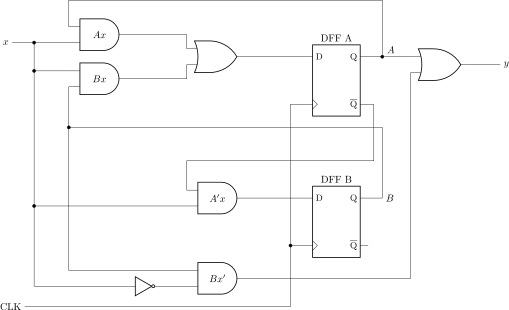
\includegraphics[width=400.8pt]{lect_6_sequential_analysis_example}\caption{circuit}\label{fig:seq-d}
\end{subfigure}
\\[6pt]
\begin{subfigure}[b]{131.8pt}\centering
  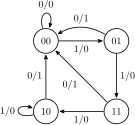
\includegraphics[width=129.8pt]{lect_6_d_state_diagram}\caption{state diagram}\label{fig:seq-d-state}
\end{subfigure}
\caption{The circuit analysed in \cref{ex:seq-d}.}
\end{figure}

\begin{example}{Analysis with JK flip-flops}{seq-jk}
In \cref{fig:seq-jk} the inputs are $J_A=B$, $K_A=Bx'$, $J_B=x'$, $K_B=A'x+Ax'=A\xor x$. With $Q(t+1)=JQ'+K'Q$,
\[
 A(t+1)=BA'+(Bx')'A,\qquad B(t+1)=x'B'+(A\xor x)'B .
\]
\Cref{tab:seq-jk} lists the flip-flop inputs for each row and the resulting next state, which gives the state diagram of \cref{fig:seq-jk-state}. (Row $AB=01$, $x=0$: $J_A=1,K_A=1$ toggles $A$ from 0 to 1, and $J_B=1,K_B=0$ sets $B$, so the next state is 11.)
\end{example}

\begin{table}[htbp]
\centering
\caption{State table of \cref{ex:seq-jk}.}
\label{tab:seq-jk}
\begin{tabular}{cc|c|cccc|cc}
\toprule
\multicolumn{2}{c|}{Present state} & Input & \multicolumn{4}{c|}{Flip-flop inputs} & \multicolumn{2}{c}{Next state}\\
$A$&$B$&$x$&$J_A$&$K_A$&$J_B$&$K_B$&$A$&$B$\\ \midrule
0&0&0&0&0&1&0&0&1\\0&0&1&0&0&0&1&0&0\\0&1&0&1&1&1&0&1&1\\0&1&1&1&0&0&1&1&0\\
1&0&0&0&0&1&1&1&1\\1&0&1&0&0&0&0&1&0\\1&1&0&1&1&1&1&0&0\\1&1&1&1&0&0&0&1&1\\ \bottomrule
\end{tabular}
\end{table}

\begin{figure}[htbp]
\centering
\begin{subfigure}[b]{295.1pt}\centering
  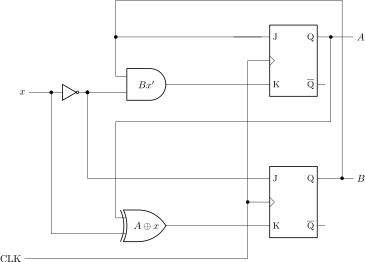
\includegraphics[width=293.1pt]{lect_6_jk_sequential_analysis}\caption{circuit}\label{fig:seq-jk}
\end{subfigure}
\\[6pt]
\begin{subfigure}[b]{137.8pt}\centering
  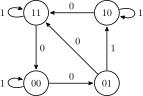
\includegraphics[width=135.8pt]{lect_6_jk_state_diagram}\caption{state diagram}\label{fig:seq-jk-state}
\end{subfigure}
\caption{The circuit analysed in \cref{ex:seq-jk}.}
\end{figure}

\begin{example}{Analysis with T flip-flops}{seq-t}
In \cref{fig:seq-t}: $T_A=Bx$, $T_B=x$ and $y=AB$. With $Q(t+1)=T\xor Q$, $A(t+1)=Bx\xor A$ and $B(t+1)=x\xor B$. The state table is \cref{tab:seq-t}. Because $y=AB$ depends on the state only, the machine is a \emph{Moore} machine and its diagram (\cref{fig:seq-t-state}) writes the output inside each state, \texttt{state/output}, and labels the arrows with the input.
\end{example}

\begin{table}[htbp]
\centering
\caption{State table of \cref{ex:seq-t}.}
\label{tab:seq-t}
\begin{tabular}{cc|c|cc|c}
\toprule
\multicolumn{2}{c|}{Present state} & Input & \multicolumn{2}{c|}{Next state} & Output\\
$A$&$B$&$x$&$A$&$B$&$y$\\ \midrule
0&0&0&0&0&0\\0&0&1&0&1&0\\0&1&0&0&1&0\\0&1&1&1&0&0\\
1&0&0&1&0&0\\1&0&1&1&1&0\\1&1&0&1&1&1\\1&1&1&0&0&1\\ \bottomrule
\end{tabular}
\end{table}

\begin{figure}[htbp]
\centering
\begin{subfigure}[b]{377.3pt}\centering
  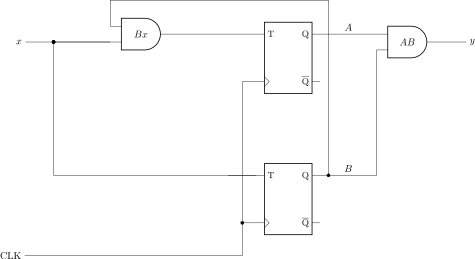
\includegraphics[width=375.3pt]{lect_6_t_sequential_analysis}\caption{circuit}\label{fig:seq-t}
\end{subfigure}
\\[6pt]
\begin{subfigure}[b]{148.8pt}\centering
  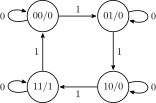
\includegraphics[width=146.8pt]{lect_6_t_state_diagram}\caption{state diagram}\label{fig:seq-t-state}
\end{subfigure}
\caption{The circuit analysed in \cref{ex:seq-t}.}
\end{figure}

\section{Mealy and Moore Models}\label{sec:mealymoore}
Synchronous sequential circuits are classified by how their outputs are generated.
\begin{itemize}
  \item In the \term{Mealy model}~\cite{mealy1955} the outputs depend on the \emph{present state and the present inputs}. In a state diagram the output is written on each transition, \texttt{input/output}. Because the output depends directly on the inputs, it can change between clock edges whenever the input changes, and may show momentary false values (glitches).
  \item In the \term{Moore model}~\cite{moore1956} the outputs depend \emph{only on the present state}. In a state diagram the output is written inside each state circle. Moore outputs change only when the state changes, which is just after a clock edge, so they are synchronous and glitch-free.
\end{itemize}
The two models are compared in detail, with timing diagrams, in \cref{sec:moore-mealy}.

\section{Design of Sequential Circuits}\label{sec:seq-design}
\termx{Design}{design} is the reverse of analysis: from a specification to a logic diagram.
\begin{enumerate}
  \item Derive a \textbf{state diagram} from the word description.
  \item Perform \textbf{state reduction}: remove states that are equivalent.
  \item Perform \textbf{state assignment}: assign a unique binary code to each state. A machine with $N$ states needs at least $\lceil\log_2N\rceil$ flip-flops.
  \item Write the binary-coded \textbf{state table}.
  \item Choose the \textbf{type of flip-flop}.
  \item Derive the simplified \textbf{flip-flop input equations} and \textbf{output equations} with K-maps (unused states give don't-cares).
  \item Draw the \textbf{logic diagram} (or write the VHDL) and verify it.
\end{enumerate}

\subsection{Example: a sequence detector}
\begin{example}{101 sequence detector}{seqdet}
Design a circuit with input $x$ and output $y$ that produces $y=1$ whenever the input sequence $101$ has just been received. Overlapping sequences count ($10101$ contains two).

\textbf{State diagram.} Three states are needed to remember how much of the pattern has been seen: $S_0$, the initial state (no useful input yet, or the last input was 0 without a preceding 1); $S_1$, the last input was 1; $S_2$, the last two inputs were 10. In $S_2$ a 1 completes the sequence: the output is 1 and, since the last input was 1, the next state is $S_1$. The output depends on the input, so this is a Mealy machine (\cref{fig:seqdet-state}).

\textbf{State assignment.} $S_0=00$, $S_1=01$, $S_2=10$; two flip-flops $A$ and $B$. The state $11$ is unused.

\textbf{State table} (\cref{tab:seqdet}).
\end{example}

\begin{table}[htbp]
\centering
\caption{State table of the 101 detector, $S_0=00$, $S_1=01$, $S_2=10$.}
\label{tab:seqdet}
\begin{tabular}{cc|c|cc|c}
\toprule
\multicolumn{2}{c|}{Present state} & Input & \multicolumn{2}{c|}{Next state} & Output\\
$A$&$B$&$x$&$A$&$B$&$y$\\ \midrule
0&0&0&0&0&0\\0&0&1&0&1&0\\0&1&0&1&0&0\\0&1&1&0&1&0\\
1&0&0&0&0&0\\1&0&1&0&1&1\\ \bottomrule
\end{tabular}
\end{table}

\figw{204.9pt}{lect_6_sequence_detector_state}{State diagram of the 101 sequence detector (Mealy).}{fig:seqdet-state}

\paragraph{Implementation with D flip-flops.} For D flip-flops the input equation is the next-state value. From K-maps of \cref{tab:seqdet} (with the unused state 11 as don't-care):
\[
 D_A = Bx',\qquad D_B = x,\qquad y = Ax .
\]
The circuit is shown in \cref{fig:seqdet-circuit}.

\figw{391.2pt}{lect_6_sequence_detector_circuit}{Logic diagram of the 101 detector with D flip-flops.}{fig:seqdet-circuit}

\paragraph{Excitation tables.} For JK and T flip-flops we need the \term{excitation table}, the inverse of the characteristic table: it states which flip-flop inputs produce a required transition $Q(t)\to Q(t+1)$ (\cref{tab:excit}). The X entries are don't-cares and are what make JK designs sometimes simpler than D designs.

\begin{table}[htbp]
\centering
\caption{Excitation tables of the JK and T flip-flops.}
\label{tab:excit}
\begin{tabular}{cc|cc}
\toprule \multicolumn{4}{c}{JK}\\ $Q(t)$&$Q(t{+}1)$&$J$&$K$\\ \midrule
0&0&0&X\\0&1&1&X\\1&0&X&1\\1&1&X&0\\ \bottomrule
\end{tabular}\qquad\qquad
\begin{tabular}{cc|c}
\toprule \multicolumn{3}{c}{T}\\ $Q(t)$&$Q(t{+}1)$&$T$\\ \midrule
0&0&0\\0&1&1\\1&0&1\\1&1&0\\ \bottomrule
\end{tabular}
\end{table}

\paragraph{Implementation with JK flip-flops.} We extend the state table with the required $J$ and $K$ inputs of each flip-flop (\cref{tab:seqdet-jk}). For flip-flop $A$: transition $0\to0$ needs $J_A=0$; $0\to1$ (row $AB=01$, $x=0$) needs $J_A=1$; $1\to0$ (both rows with $AB=10$) needs $K_A=1$. For flip-flop $B$: $0\to1$ occurs when $x=1$ in states 00 and 10; $1\to0$ in state 01 when $x=0$; $1\to1$ in state 01 when $x=1$. The K-maps (the unused state 11 and all entries X are don't-cares) give
\[
 J_A = Bx',\qquad K_A = 1,\qquad J_B = x,\qquad K_B = x',\qquad y = Ax .
\]
Note that $K_A$ is the constant 1: in state $10$ the flip-flop $A$ must always return to 0, whatever the input, and in all other states the value of $K_A$ is a don't-care. The flip-flop input logic of the JK design is thus one AND gate and one inverter (shared by $J_A$ and $K_B$), the same as for the D design; the advantage of JK flip-flops appears in larger machines, where the don't-cares often remove literals.

\begin{table}[htbp]
\centering
\caption{Excitation table for the 101 detector with JK flip-flops.}
\label{tab:seqdet-jk}
\begin{tabular}{cc|c|cc|cc|cc}
\toprule
\multicolumn{2}{c|}{PS} & Input & \multicolumn{2}{c|}{NS} & \multicolumn{2}{c|}{$A$ inputs} & \multicolumn{2}{c}{$B$ inputs}\\
$A$&$B$&$x$&$A$&$B$&$J_A$&$K_A$&$J_B$&$K_B$\\ \midrule
0&0&0&0&0&0&X&0&X\\0&0&1&0&1&0&X&1&X\\
0&1&0&1&0&1&X&X&1\\0&1&1&0&1&0&X&X&0\\
1&0&0&0&0&X&1&0&X\\1&0&1&0&1&X&1&1&X\\ \bottomrule
\end{tabular}
\end{table}

\paragraph{VHDL descriptions.} In VHDL a machine is best described with an \emph{enumerated type} for the states, e.g.\ \code{type state_type is (S0, S1, S2);}; the synthesis tool then chooses the state encoding (binary, one-hot, \dots). \Cref{lst:seqdet-fsm} describes the detector with two processes: a clocked process holding the state register and a combinational process computing the next state and the output. \Cref{lst:seqdet-struct} is the gate-level (structural) description that follows the D-flip-flop design.

\vhdlfile{listings/ch06_seq_detector_fsm.vhd}{The 101 detector as a state machine with an enumerated state type.}{lst:seqdet-fsm}
\vhdlfile{listings/ch06_seq_detector_struct.vhd}{The 101 detector as two D flip-flops and gates (structural description).}{lst:seqdet-struct}

\subsection{Example: a binary counter with T flip-flops}
\begin{example}{3-bit binary counter}{counter3}
Design a counter that cycles through $000,001,\dots,111$ and back to $000$, using T flip-flops. There are no inputs except the clock.

\textbf{Solution.} A T flip-flop must toggle ($T=1$) exactly when its bit changes between the present and next states. In the table, $A_0$ changes every clock; $A_1$ changes when $A_0=1$; $A_2$ changes when $A_1=A_0=1$ (\cref{tab:counter3}). Hence
\[
 T_{A_0}=1,\qquad T_{A_1}=A_0,\qquad T_{A_2}=A_1A_0 .
\]
The circuit (\cref{fig:counter3}) uses three flip-flops and one AND gate.
\end{example}

\begin{table}[htbp]
\centering
\caption{State table and T inputs of the 3-bit counter.}
\label{tab:counter3}
\begin{tabular}{ccc|ccc|ccc}
\toprule
\multicolumn{3}{c|}{Present state} & \multicolumn{3}{c|}{Next state} & \multicolumn{3}{c}{Flip-flop inputs}\\
$A_2$&$A_1$&$A_0$&$A_2$&$A_1$&$A_0$&$T_{A_2}$&$T_{A_1}$&$T_{A_0}$\\ \midrule
0&0&0&0&0&1&0&0&1\\0&0&1&0&1&0&0&1&1\\0&1&0&0&1&1&0&0&1\\0&1&1&1&0&0&1&1&1\\
1&0&0&1&0&1&0&0&1\\1&0&1&1&1&0&0&1&1\\1&1&0&1&1&1&0&0&1\\1&1&1&0&0&0&1&1&1\\ \bottomrule
\end{tabular}
\end{table}

\figw{314.0pt}{lect_6_t_3bit_counter}{A 3-bit binary counter with T flip-flops.}{fig:counter3}

\begin{chaptersummary}
\begin{itemize}
  \item A \textbf{sequential circuit} contains memory; its output depends on the inputs and the \textbf{state}. \textbf{Synchronous} circuits change state at clock edges, using flip-flops.
  \item \textbf{Latches} (SR, $\overline{S}\overline{R}$, gated SR, D) are level-triggered. \textbf{Flip-flops} (D, JK, T) are edge-triggered. Characteristic equations: $Q^+=D$; $Q^+=JQ'+K'Q$; $Q^+=T\xor Q$; $Q^+=S+R'Q$ ($SR=0$).
  \item \textbf{Asynchronous} reset overrides the clock; \textbf{synchronous} reset acts at the clock edge. In VHDL, \code{rising_edge(clk)} describes a flip-flop.
  \item \textbf{Analysis}: logic diagram $\to$ flip-flop input equations $\to$ next-state equations $\to$ state table $\to$ state diagram.
  \item \textbf{Mealy}: output depends on state and input. \textbf{Moore}: output depends on state only.
  \item \textbf{Design}: word problem $\to$ state diagram $\to$ (reduction) $\to$ state assignment $\to$ state table $\to$ excitation $\to$ flip-flop input equations $\to$ logic diagram. Use the \textbf{excitation tables} for JK and T flip-flops.
\end{itemize}
\end{chaptersummary}

\chapsec{Exercises}
\begin{exlist}
  \item \textbf{Next-state equations.} A sequential circuit has two D flip-flops $A$, $B$ and an input $x$, with $D_A=Ax+Bx$ and $D_B=A'x$. Write the next-state equations $A(t+1)$ and $B(t+1)$.
  \item \textbf{State diagram.} A circuit has one T flip-flop and an input $x$, with $T=A\xor x$. Draw the state diagram. Describe what the circuit does.
  \item \textbf{JK flip-flop behaviour.} A JK flip-flop has $J=K=1$ permanently. (a)~Describe how $Q$ changes on each clock pulse. (b)~Draw its state diagram. (c)~If the clock frequency is 1~MHz, what is the frequency of $Q$?
  \item \textbf{Mealy or Moore?} ``A sequence detector produces $y=1$ whenever the internal counter holds the value 101. The output remains 1 as long as the counter is in this state, regardless of the input during that clock cycle.'' Classify the machine and justify your answer.
  \item An NOR SR latch initially has $Q=0$. The inputs $(S,R)$ are applied in turn: $(0,0)$, $(1,0)$, $(0,0)$, $(0,1)$, $(0,0)$. Give $Q$ after each step.
  \item Explain why a D latch cannot be used directly in place of a D flip-flop in a counter in which $Q'$ is fed back to $D$. What happens while the latch is transparent?
  \item Show how to build (a)~a T flip-flop and (b)~a D flip-flop from a JK flip-flop.
  \item Derive the characteristic equation $Q(t+1)=S+R'Q$ of the SR flip-flop from its characteristic table, with a K-map in which the combination $S=R=1$ is a don't-care.
  \item \textbf{Analysis.} A circuit has two D flip-flops with $D_A=x\xor B$, $D_B=A$ and output $y=AB'$. Draw the state table and state diagram. Is it a Mealy or a Moore machine?
  \item \textbf{Design.} Design a Mealy sequence detector with input $x$ and output $y$ that detects the sequence $110$ (overlapping allowed) using two D flip-flops with the state assignment $S_0=00$, $S_1=01$, $S_2=10$. Give the state diagram, the state table, the equations, and the VHDL of the machine.
  \item Design a 3-bit binary counter with JK flip-flops.
  \item How many flip-flops are required to implement a state machine with (a)~5 states; (b)~9 states; (c)~a one-hot encoding of 9 states?
  \item Write VHDL for a D flip-flop with synchronous reset and an enable input \code{en}: the register loads \code{D} only when \code{en = '1'}.
  \item Write the VHDL of an 8-bit register with asynchronous active-low reset.
\end{exlist}

\chapsec{Further Reading}
The treatment of latches, flip-flops and the analysis and design of clocked sequential circuits follows Chapter~5 of Mano and Ciletti~\cite{mano2018}. Brown and Vranesic~\cite{brown2009} (Chapters~7 and~8) and Wakerly~\cite{wakerly2006} discuss timing parameters (setup, hold, propagation delay) in detail, which we have not covered. Mealy~\cite{mealy1955} and Moore~\cite{moore1956} introduced the two models. For VHDL coding style for registers and state machines, see Ashenden~\cite{ashenden2008}.

\chapter{Registers and Counters}\label{ch:registers}

\begin{objectives}
After studying this chapter you will be able to:
\begin{itemize}
  \item design registers with parallel load and shift registers, and describe serial transfer and serial addition;
  \item describe a universal shift register and write it in VHDL;
  \item explain the operation, delay and frequency limit of asynchronous (ripple) counters;
  \item design synchronous binary counters, up/down counters and counters with parallel load;
  \item build modulo-$N$ counters, including the BCD counter, and make a counter self-correcting;
  \item use ring counters and counter--decoder combinations to generate timing signals.
\end{itemize}
\end{objectives}

\section{Registers}\label{sec:registers}
A \term{register} is a group of flip-flops, each of which stores one bit. An $n$-bit register consists of $n$ flip-flops sharing one clock and stores one $n$-bit word. The simplest register (\cref{fig:reg4}) is a row of D flip-flops: at each clock edge the four inputs are copied to the outputs. Registers may also contain gates that control \emph{how} and \emph{when} new information is accepted.

\figw{403.1pt}{lect_7_4bit_register_diagram}{A 4-bit register built from D flip-flops.}{fig:reg4}

\subsection{Register with parallel load}
Transferring new information into a register is called \term{loading}; if all bits are transferred at the same moment it is a \term{parallel load}. A register that loads on every clock pulse cannot hold its data. A \emph{load} control input solves this (\cref{fig:regload}): a 2-to-1 multiplexer at each flip-flop input selects either the external data $I_i$ (when $\mathit{Load}=1$) or the flip-flop's own output (when $\mathit{Load}=0$), so that the register keeps its value through the feedback path. Equivalently, the clock may be \emph{gated}, but this is poor practice in synchronous design because it can introduce clock skew and glitches; a multiplexer (or a flip-flop with a clock-enable input) is preferred.

\figside{509.4pt}{lect_7_4bit_register_parallel_load}{A 4-bit register with parallel load. When $\mathit{Load}=0$ the flip-flops recirculate their own outputs.}{fig:regload}

\section{Shift Registers}\label{sec:shift}
A \term{shift register} can move its stored bits to the left or right. The simplest one is a chain of D flip-flops in which the output of each is connected to the input of the next and all flip-flops share a clock (\cref{fig:shift}). At each clock pulse every bit moves one position along the chain, and a new bit enters at the \emph{serial input}. Because all flip-flops change simultaneously, each captures the \emph{old} output of its neighbour, which is why the data moves exactly one position and not through the whole chain.

\figw{401.6pt}{lect_7_4bit_shift_register}{A 4-bit shift register: serial input at the left, serial output at the right.}{fig:shift}

\subsection{Serial transfer}
In a \term{serial transfer}, information is moved from a register $A$ to a register $B$ one bit at a time: the serial output of $A$ is connected to the serial input of $B$, and both registers are clocked together (\cref{fig:sertrans}). After $n$ clock pulses the $n$-bit word has been transferred. If the serial output of $A$ is also fed back to its own serial input, $A$ is \emph{rotated} and keeps its data. \Cref{tab:sertrans} traces the transfer of $A=\bin{1011}$, and \cref{fig:sertrans-timing} is the timing diagram; a serial transfer needs far fewer wires than a parallel transfer, but takes $n$ clock periods instead of one.

\begin{figure}[htbp]
\centering
\begin{subfigure}[b]{234.3pt}\centering
  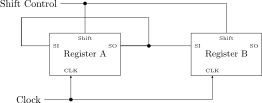
\includegraphics[width=232.3pt]{lect_7_serial_transfer}\caption{circuit}\label{fig:sertrans}
\end{subfigure}
\\[6pt]
\begin{subfigure}[b]{282.8pt}\centering
  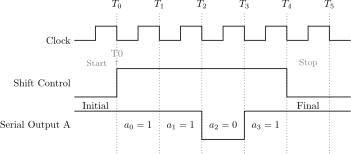
\includegraphics[width=280.8pt]{lect_7_serial_transfer_timing}\caption{timing diagram}\label{fig:sertrans-timing}
\end{subfigure}
\caption{Serial transfer from register $A$ to register $B$.}
\end{figure}

\begin{table}[htbp]
\centering
\caption{Serial transfer of $A=\bin{1011}$ into $B$ ($A$ is rotated).}
\label{tab:sertrans}
\begin{tabular}{lccc}
\toprule
Timing pulse & Serial output & Register $A$ & Register $B$\\ \midrule
Initial & --- & 1011 & 0000\\
$T_1$ & 1 & 1101 & 1000\\
$T_2$ & 1 & 1110 & 1100\\
$T_3$ & 0 & 0111 & 0110\\
$T_4$ & 1 & 1011 & 1011\\ \bottomrule
\end{tabular}
\end{table}

\subsection{Serial adder}
A \term{serial adder} adds two binary numbers one bit at a time, using one full adder instead of $n$ (\cref{fig:seradd}). Two shift registers hold the operands $A$ (augend) and $B$ (addend); at each clock pulse the least significant bits of both registers and a stored carry are added by the full adder; the sum bit is shifted into the most significant end of $A$ (so that the sum replaces the augend); $B$ is rotated to preserve its value; and the carry-out is stored in a D flip-flop for the next bit position. The flip-flop is cleared to 0 initially. \Cref{tab:seradd} traces $A=\bin{1001}$ (9) plus $B=\bin{0011}$ (3): after four pulses $A=\bin{1100}=12$. The adder is slow ($n$ clock periods) but needs very little hardware.

\figw{273.1pt}{lect_7_serial_adder}{A serial adder: one full adder and a carry flip-flop.}{fig:seradd}

\begin{table}[htbp]
\centering
\caption{Trace of the serial addition $1001+0011$.}
\label{tab:seradd}
\begin{tabular}{lcc|ccc|cc}
\toprule
Pulse & Reg.\ $A$ & Reg.\ $B$ & $x$ & $y$ & $C_{in}$ & $S$ & $C_{out}$\\ \midrule
Initial & 1001 & 0011 & --- & --- & 0 & --- & ---\\
$T_1$ & 0100 & 1001 & 1 & 1 & 0 & 0 & 1\\
$T_2$ & 0010 & 1100 & 0 & 1 & 1 & 0 & 1\\
$T_3$ & 1001 & 0110 & 0 & 0 & 1 & 1 & 0\\
$T_4$ & 1100 & 0011 & 1 & 0 & 0 & 1 & 0\\ \bottomrule
\end{tabular}

\smallskip
{\small $x$ and $y$ are the bits of $A$ and $B$ added in each step (before the shift); the registers show their contents after the pulse.}
\end{table}

\subsection{Universal shift register}
A \term{universal shift register} combines several operations in one register: clear, shift right, shift left, parallel load and no change. Two mode inputs $s_1s_0$ select the operation (\cref{tab:usr}). In the implementation (\cref{fig:usr}) a 4-to-1 multiplexer at the input of each flip-flop selects among its own output (hold), its left neighbour (shift right), its right neighbour (shift left) and the parallel input. \Cref{lst:usr} is a behavioural VHDL description: the concatenation operator \code{&} builds the shifted word, e.g.\ \code{SR_IN & reg_val(3 downto 1)} places the serial input in the MSB and drops the LSB.

\begin{table}[htbp]
\centering
\caption{Function table of a 4-bit universal shift register ($A_i^+$ is the next value of $A_i$).}
\label{tab:usr}
\begin{tabular}{cc|l|cccc}
\toprule
$s_1$&$s_0$&Operation&$A_3^+$&$A_2^+$&$A_1^+$&$A_0^+$\\ \midrule
0&0&no change&$A_3$&$A_2$&$A_1$&$A_0$\\
0&1&shift right&SIR&$A_3$&$A_2$&$A_1$\\
1&0&shift left&$A_2$&$A_1$&$A_0$&SIL\\
1&1&parallel load&$I_3$&$I_2$&$I_1$&$I_0$\\ \bottomrule
\end{tabular}
\end{table}

\begin{sidewaysfigure}[htbp]
\centering
\begin{subfigure}[b]{363.5pt}\centering
  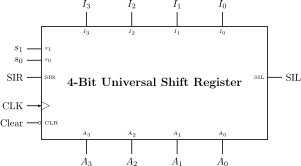
\includegraphics[width=361.5pt]{lect_7_universal_shift_register_block}\caption{block diagram}
\end{subfigure}
\caption{A 4-bit universal shift register.}\label{fig:usr}
\end{sidewaysfigure}

\begin{sidewaysfigure}[htbp]
\centering
\ContinuedFloat
\begin{subfigure}[b]{602.0pt}\centering
  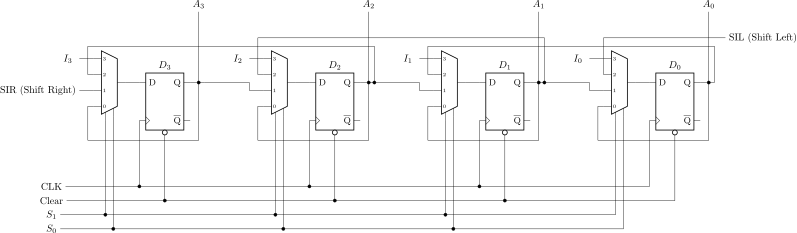
\includegraphics[width=600.0pt]{lect_7_universal_shift_register}\caption{implementation with multiplexers}
\end{subfigure}
\caption[]{A 4-bit universal shift register.}
\end{sidewaysfigure}

\vhdlfile{listings/ch07_universal_shift_register.vhd}{Behavioural VHDL of a 4-bit universal shift register with asynchronous clear.}{lst:usr}

\begin{keypoint}[Shifts are multiplications]
Shifting an unsigned binary number one place to the left multiplies it by 2 (provided no 1 is shifted out), and shifting right with a 0 entering the MSB divides it by 2 (discarding the remainder). Shifters are therefore used to multiply and divide by powers of two, and in the shift-and-add algorithms for multiplication.
\end{keypoint}

\section{Counters}\label{sec:counters}
A \term{counter} is a register that goes through a predetermined sequence of states when it is driven by input pulses, most often the clock. The sequence can be a binary count or any other. Counters are classified by how the clock reaches the flip-flops (\cref{fig:counter-block}):
\begin{itemize}
  \item in a \term{ripple} (asynchronous) counter, the output of one flip-flop clocks the next, so there is no common clock;
  \item in a \term{synchronous} counter, a common clock drives all flip-flops simultaneously.
\end{itemize}

\figw{247.9pt}{lect_7_counter_block}{General $n$-bit counter.}{fig:counter-block}

\subsection{Ripple counters}
In a \term{ripple counter} the clock is applied only to the first flip-flop, and the output of each flip-flop provides the clock of the next (\cref{fig:ripple}). Each stage is a T flip-flop with $T=1$ (a JK flip-flop with $J=K=1$), so each stage divides the frequency of its clock by 2, and the outputs form a binary count. The counter is very simple, but it is slower than a synchronous counter because the changes propagate, or ``ripple'', along the chain.

\figw{398.6pt}{lect_7_4bit_ripple_counter}{A 4-bit binary ripple counter built from T flip-flops with $T=1$.}{fig:ripple}

\paragraph{Characteristics.} The flip-flops change one after another, not together (\cref{fig:ripple-timing}).
\begin{itemize}
  \item \textbf{Propagation delay.} Each flip-flop has a delay $t_{pd}$ between a clock edge and the change of its output; in a ripple counter the delays add, so an $n$-bit counter needs up to $n\,t_{pd}$ to settle after a clock edge.
  \item \textbf{Glitches.} While the counter ripples to its final state, the outputs pass through \emph{invalid intermediate states} (for example $0111\to0110\to0100\to0000$ when counting from 7 to 8). Combinational logic or decoders connected to the outputs may see these states and produce momentary false outputs.
  \item \textbf{Frequency limit.} The next clock edge must not arrive before the previous ripple has finished: $f_{clk} < 1/(n\,t_{pd})$.
\end{itemize}
For example, a 4-bit ripple counter with $t_{pd}=10$~ns per stage settles in at most 40~ns, so the clock must be slower than 25~MHz.

\figw{243.5pt}{lect_7_4bit_ripple_counter_timing}{Timing diagram of a ripple counter: each flip-flop changes a delay after the previous one.}{fig:ripple-timing}

\subsection{BCD ripple counter}
A \term{BCD counter} counts from 0 to 9 ($\bin{0000}$ to $\bin{1001}$) and returns to 0 (\cref{fig:bcd-state}). BCD counters are essential in instruments and clocks that display decimal digits. A BCD ripple counter is obtained from the binary ripple counter by modifying two stages so that the state $1001$ is followed by $0000$ and states 10--15 are skipped (\cref{fig:bcd-ripple}).
\begin{itemize}
  \item The $J$ input of the $Q_1$ flip-flop is connected to $\overline{Q_3}$. When the count reaches $1000$ ($Q_3=1$), $J=0$ and $Q_1$ cannot toggle to 1 on the next pulse, so the sequence $1001\to1010$ never occurs.
  \item The $J$ input of the $Q_3$ flip-flop is connected to $Q_2Q_1$, so $Q_3$ sets only on the transition $0111\to1000$; $Q_3$ is reset on the transition $1001\to0000$ by its own $K=1$.
\end{itemize}

\begin{figure}[htbp]
\centering
\begin{subfigure}[b]{253.3pt}\centering
  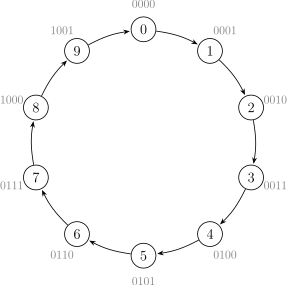
\includegraphics[width=251.3pt]{lect_7_bcd_state_diagram}\caption{state diagram}\label{fig:bcd-state}
\end{subfigure}
\\[6pt]
\begin{subfigure}[b]{412.0pt}\centering
  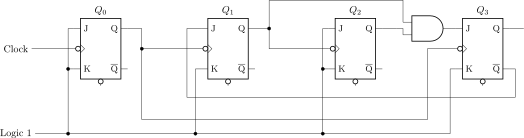
\includegraphics[width=410.0pt]{lect_7_bcd_ripple_counter}\caption{BCD ripple counter}\label{fig:bcd-ripple}
\end{subfigure}
\caption{The BCD counter.}
\end{figure}

\subsection{Synchronous binary counters}
In a \term{synchronous counter} all flip-flops are clocked together, and combinational logic at the $J$, $K$ or $T$ inputs decides which of them toggle. There is no accumulation of delays, so synchronous counters are used for high frequencies. They are designed with the standard procedure of \cref{sec:seq-design}. From the 3-bit design of \cref{ex:counter3} we know that in a binary up-counter a bit toggles when \emph{all lower-order bits are 1}:
\[
 T_{A_i} = A_{i-1}A_{i-2}\cdots A_0,\quad T_{A_0}=1 .
\]
\Cref{fig:sync} shows the 4-bit counter: the toggle condition of each stage is formed by a chain of AND gates. The delay of a synchronous counter is therefore the flip-flop delay plus the delay of one AND chain, independent of the number of bits if wider AND gates or a lookahead structure are used.

\figside{542.9pt}{lect_7_4bit_synchronous_counter}{A 4-bit synchronous binary counter with T flip-flops.}{fig:sync}

\subsection{Up/down counter}
An \term{up/down counter} counts up when $\mathit{Up}=1$ and down when $\mathit{Down}=1$ (\cref{fig:updown-state}). In the down direction a bit toggles when all lower-order bits are 0, so
\[
 T_{A_i} = \mathit{Up}\cdot A_{i-1}\cdots A_0 \;+\; \mathit{Down}\cdot \NOT{A_{i-1}}\cdots\NOT{A_0}.
\]
\Cref{fig:updown} shows the circuit.

\begin{sidewaysfigure}[htbp]
\centering
\begin{subfigure}[b]{359.5pt}\centering
  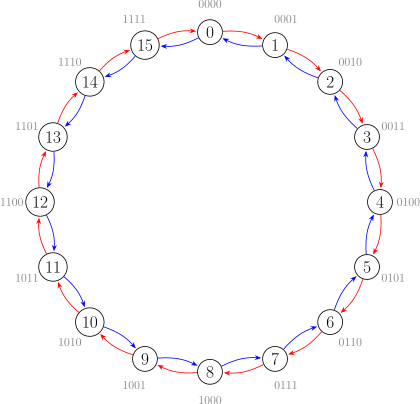
\includegraphics[width=357.5pt]{lect_7_4bit_up_down_counter_state_diagram}\caption{state diagram}\label{fig:updown-state}
\end{subfigure}
\caption{Up/down counter.}
\end{sidewaysfigure}

\begin{sidewaysfigure}[htbp]
\centering
\ContinuedFloat
\begin{subfigure}[b]{514.6pt}\centering
  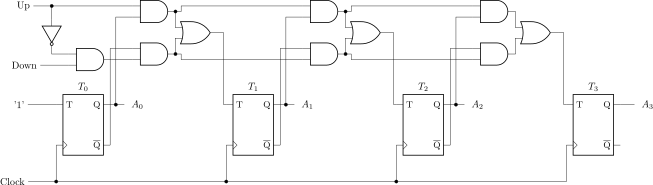
\includegraphics[width=512.6pt]{lect_7_4bit_up_down_counter}\caption{4-bit synchronous up/down counter}\label{fig:updown}
\end{subfigure}
\caption[]{Up/down counter.}
\end{sidewaysfigure}

\subsection{Counter with parallel load}
Counters in digital systems often need to be preset to a given value as well as counted. \Cref{tab:cnt-load} gives the function table of a counter with \emph{clear}, \emph{load} and \emph{count} controls (\cref{fig:cnt-load}), with a priority order: clear first, then load, then count. \Cref{lst:cnt-load} is the VHDL; the type \code{unsigned} of the package \code{numeric_std} allows the expression \code{count_val + 1}.

\begin{table}[htbp]
\centering
\caption{Function table of a 4-bit counter with parallel load (the clear is asynchronous and active-high in the VHDL of \cref{lst:cnt-load}).}
\label{tab:cnt-load}
\begin{tabular}{cccc|l}
\toprule
Clear & CLK & Load & Count & Function\\ \midrule
1 & X & X & X & clear to 0\\
0 & $\uparrow$ & 1 & X & load parallel inputs\\
0 & $\uparrow$ & 0 & 1 & count up\\
0 & $\uparrow$ & 0 & 0 & no change\\ \bottomrule
\end{tabular}
\end{table}

\figw{410.0pt}{lect_7_counter_parallel_load}{A 4-bit counter with parallel load.}{fig:cnt-load}

\vhdlfile{listings/ch07_counter_parallel_load.vhd}{VHDL of a 4-bit counter with asynchronous clear, parallel load and count enable.}{lst:cnt-load}

\subsection{Modulo-$N$ counters}
A \term{modulo-$N$ counter} goes through a repeating sequence of $N$ states and so divides the clock frequency by $N$. The BCD counter is a modulo-10 counter. A modulo-$N$ counter can be built from a binary counter with parallel load or clear in two ways (\cref{fig:bcd-load}):
\begin{itemize}
  \item \textbf{synchronous load}: detect the last count (for BCD, $9=\bin{1001}$) and, on the \emph{next clock edge}, load $\bin{0000}$; the count 9 appears for a full clock period;
  \item \textbf{asynchronous clear}: detect the first \emph{invalid} count ($10=\bin{1010}$) and clear the counter \emph{immediately}; the state 10 appears for a brief moment (a glitch) before the counter resets, which may disturb other circuits.
\end{itemize}
The synchronous method is cleaner. For BCD the detection of 9 needs only $Q_3Q_0$ since 9 is the only count between 0 and 9 with both bits 1.

\begin{figure}[htbp]
\centering
\begin{subfigure}[b]{203.7pt}\centering
  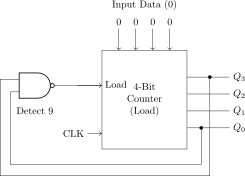
\includegraphics[width=201.7pt]{lect_7_bcd_counter_sync_load}\caption{synchronous load (detect 9)}
\end{subfigure}
\\[6pt]
\begin{subfigure}[b]{207.4pt}\centering
  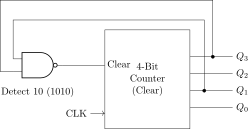
\includegraphics[width=205.4pt]{lect_7_bcd_counter_async_clear}\caption{asynchronous clear (detect 10)}
\end{subfigure}
\caption{Two ways of making a BCD counter from a binary counter,.}\label{fig:bcd-load}
\end{figure}

\figw{225.2pt}{lect_7_modulo_n_counter}{Block diagram of a modulo-$N$ counter.}{fig:modn}

\subsection{Self-correcting counters}
A counter with \emph{unused} states can enter one of them by noise or at power-up. If there is no path out of the unused states, the counter is stuck. A \term{self-correcting} design makes sure that every unused state eventually leads to a valid state. In the modulo-6 counter of \cref{fig:selfcorr} the unused states 110 and 111 both lead to 000 (\cref{tab:selfcorr}). Note that don't-cares used during minimisation must be checked afterwards: the next states of the unused states are whatever the simplified equations produce.

\begin{table}[htbp]
\centering
\caption{State table of the self-correcting modulo-6 counter.}
\label{tab:selfcorr}
\begin{tabular}{ccc|ccc}
\toprule
$Q_2$&$Q_1$&$Q_0$&$Q_2^+$&$Q_1^+$&$Q_0^+$\\ \midrule
0&0&0&0&0&1\\0&0&1&0&1&0\\0&1&0&0&1&1\\0&1&1&1&0&0\\1&0&0&1&0&1\\1&0&1&0&0&0\\ \midrule
1&1&0&0&0&0\\1&1&1&0&0&0\\ \bottomrule
\end{tabular}
\end{table}

\figw{172.8pt}{lect_7_self_correcting_counter}{State diagram of the self-correcting modulo-6 counter.}{fig:selfcorr}

\subsection{Ring counters}
A \term{ring counter} is a circular shift register in which a single 1 circulates (\cref{fig:ring}): it is initialised to $1000$ and the 1 moves one place at every pulse, producing the sequence of \cref{tab:ring}. An $n$-bit ring counter has $n$ states, and the output of each flip-flop is high for one clock period out of $n$, so the outputs are $n$ non-overlapping timing signals (\cref{fig:timing}) with no decoder needed. Each output has a frequency $f_{clk}/n$. A \term{Johnson} (twisted-ring) counter feeds back the \emph{complement} of the last output instead, which doubles the number of states to $2n$ at the cost of a decoder.

\begin{table}[htbp]
\centering
\caption{Sequence of a 4-bit ring counter.}
\label{tab:ring}
\begin{tabular}{c|cccc}
\toprule Clock & $T_0$&$T_1$&$T_2$&$T_3$\\ \midrule
$t_0$&1&0&0&0\\$t_1$&0&1&0&0\\$t_2$&0&0&1&0\\$t_3$&0&0&0&1\\$t_4$&1&0&0&0\\ \bottomrule
\end{tabular}
\end{table}

\begin{figure}[htbp]
\centering
\begin{subfigure}[b]{191.1pt}\centering
  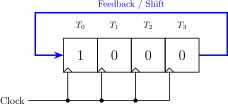
\includegraphics[width=189.1pt]{lect_7_ring_counter}\caption{4-bit ring counter}\label{fig:ring}
\end{subfigure}
\\[6pt]
\begin{subfigure}[b]{293.0pt}\centering
  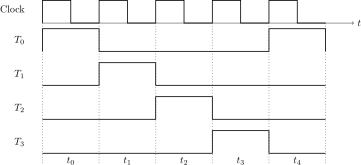
\includegraphics[width=291.0pt]{lect_7_timing_signals}\caption{timing signals}\label{fig:timing}
\end{subfigure}
\caption{Ring counter and the timing signals it generates.}
\end{figure}

\subsection{Application: generating timing signals}
Controllers need timing signals that start the successive steps of an operation. Two methods are common (\cref{fig:timing-gen}):
\begin{enumerate}
  \item a \textbf{ring counter}: $N$ flip-flops give $N$ signals directly, with no decoding, glitch-free and fast, but it needs many flip-flops;
  \item a \textbf{counter and decoder}: an $n$-bit binary counter followed by an $n$-to-$2^n$ decoder gives $N=2^n$ signals with only $n$ flip-flops, at the cost of the decoder gates (and, with a ripple counter, glitches).
\end{enumerate}
For 16 signals the ring counter needs 16 flip-flops, whereas the counter and decoder need 4 flip-flops and a 4-to-16 decoder. Timing signals of this kind drive the control unit of the processors in \cref{ch:dedicated,ch:gp}.

\begin{figure}[htbp]
\centering
\begin{subfigure}[b]{228.4pt}\centering
  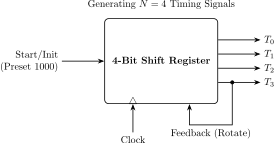
\includegraphics[width=226.4pt]{lect_7_ring_counter_generator}\caption{ring counter}
\end{subfigure}
\\[6pt]
\begin{subfigure}[b]{278.1pt}\centering
  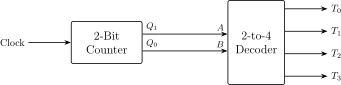
\includegraphics[width=276.1pt]{lect_7_counter_decoder_block}\caption{counter and decoder}
\end{subfigure}
\caption{Two timing-signal generators.}\label{fig:timing-gen}
\end{figure}

\begin{chaptersummary}
\begin{itemize}
  \item A \textbf{register} is a group of flip-flops; \textbf{parallel load} uses a multiplexer at each input to choose between new data and hold.
  \item A \textbf{shift register} moves its bits one place per clock; serial transfer and the \textbf{serial adder} (one full adder and a carry flip-flop) take $n$ clock periods. The \textbf{universal shift register} supports hold, shift right, shift left and load.
  \item \textbf{Ripple counters} are simple but their delays accumulate ($f_{clk}<1/(n\,t_{pd})$) and they glitch. \textbf{Synchronous counters} toggle bit $i$ when all lower bits are 1 ($T_i=A_{i-1}\cdots A_0$).
  \item \textbf{Up/down counters} combine both toggle conditions. \textbf{Counters with parallel load} can be preset and truncated: a modulo-$N$ counter uses synchronous load (detect $N-1$) or asynchronous clear (detect $N$).
  \item \textbf{Self-correcting} counters guarantee that unused states lead to a valid state.
  \item A \textbf{ring counter} generates $N$ timing signals with $N$ flip-flops; a counter with a decoder uses only $\log_2N$ flip-flops.
\end{itemize}
\end{chaptersummary}

\chapsec{Exercises}
\begin{exlist}
  \item \textbf{Register design.} Design a 4-bit register with inputs \code{CLK}, \code{CLR}, \code{LD}, \code{INC} and \code{I[3:0]}. \code{CLR = 1} resets it to \bin{0000} at the clock edge; \code{LD = 1} loads \code{I} (with priority over \code{INC}); \code{INC = 1} increments it; otherwise it holds its value. Write the behavioural VHDL.
  \item \textbf{Shift register analysis.} A 4-bit universal shift register (\cref{tab:usr}) initially holds $\bin{1010}$. Find its content after (a)~shift right with $\mathrm{SIR}=1$; then (b)~shift left with $\mathrm{SIL}=0$; then (c)~no change; then (d)~parallel load of $I=\bin{1100}$.
  \item \textbf{Counter design.} Design a synchronous modulo-6 counter (sequence 0, 1, 2, 3, 4, 5, 0, \dots) with JK flip-flops. Draw the state diagram and the excitation table, and find the $J$ and $K$ equations. Does the counter correct itself from the unused states 6 and 7?
  \item \textbf{Timing diagram.} Draw the timing diagram of a 4-bit ring counter initially in the state $\bin{1000}$ ($Q_3=1$) for five clock pulses. What is the relation between the frequency of a single output $Q_i$ and the clock frequency? How does a Johnson counter differ?
  \item Trace the serial transfer of $A=\bin{1100}$ into a register $B$ initially $\bin{0000}$ (as in \cref{tab:sertrans}), with $A$ rotating. What do $A$ and $B$ contain after four pulses?
  \item Trace the serial addition of $A=\bin{0110}$ and $B=\bin{0101}$ in the format of \cref{tab:seradd}, and give the sum.
  \item A 4-bit ripple counter uses flip-flops with $t_{pd}=10$~ns. What is the highest clock frequency, and what is the worst-case settling time when the counter changes from 0111 to 1000?
  \item Show how to use a 4-bit counter with synchronous parallel load to make a BCD counter. Give the load condition and the data inputs.
  \item Derive the $T$ input equations of a 3-bit synchronous \emph{up/down} counter with control inputs $\mathit{Up}$ and $\mathit{Down}$.
  \item You need eight timing signals. Compare (a)~a ring counter and (b)~a counter and decoder in terms of the number of flip-flops and other gates.
  \item A 4-bit universal shift register contains the unsigned number 0011 (3). What number does it hold after one shift left with $\mathrm{SIL}=0$? What is the effect on a number if the shift-left is applied $k$ times? What does a shift right with $\mathrm{SIR}=0$ do to $\bin{0110}$?
  \item Write VHDL for an 8-bit shift register with serial input \code{sin}, serial output \code{sout}, a clock and a shift-enable input \code{en}.
  \item Write the VHDL of a modulo-10 counter that counts 0--9 (4-bit output) using \code{unsigned} arithmetic and a synchronous reset to 0 after 9.
  \item Explain, with a timing sketch, how an asynchronous-clear BCD counter can produce a short glitch on the output $Q_1$ when it passes through the state 10.
\end{exlist}

\chapsec{Further Reading}
Registers and counters are covered in Chapter~6 of Mano and Ciletti~\cite{mano2018} and in Chapter~7 of Brown and Vranesic~\cite{brown2009}, which also treat Johnson counters and the VHDL of counters in more detail; see also Wakerly~\cite{wakerly2006} for the design of synchronous counters and a thorough treatment of the timing of ripple counters.

\chapter{Finite State Machines}\label{ch:fsm}

\begin{objectives}
After studying this chapter you will be able to:
\begin{itemize}
  \item describe a finite state machine (FSM) by its next-state logic, state memory and output logic, and distinguish the Moore from the Mealy model;
  \item analyse an FSM from its circuit and synthesise one from a word description, using state diagrams, state tables and K-maps;
  \item apply the design procedure to counters, controllers and one-shot circuits;
  \item write FSMs in VHDL with the two-process method and the \code{numeric_std} type conversions;
  \item compare Moore and Mealy implementations of the same function, in the number of states, the output timing and the risk of glitches; and
  \item state the clock-period constraint of a synchronous FSM and choose a state encoding.
\end{itemize}
\end{objectives}

\section{Finite State Machines}\label{sec:fsm-recall}
A \term{finite state machine} (FSM) is a computational model with a finite number of \emph{states}; it moves between states according to its inputs and its present state, and produces outputs. Every synchronous sequential circuit of \cref{ch:latches} is an FSM, and an FSM is the standard way to describe a controller. It has three parts (\cref{fig:fsm-general}):
\begin{enumerate}
  \item \textbf{next-state logic}, a combinational circuit that computes the next state from the present state and the inputs;
  \item \textbf{state memory}, the flip-flops (the \term{state register}) that hold the present state and are updated at each clock edge; and
  \item \textbf{output logic}, a combinational circuit that generates the outputs.
\end{enumerate}

\figside{461.1pt}{lect_8_fsm_general_block_diagram}{General structure of an FSM: next-state logic, state register and output logic.}{fig:fsm-general}

\section{Moore and Mealy Machines}\label{sec:models}
The two FSM models differ in their output logic (\cref{fig:mealy-moore}).
\begin{itemize}
  \item \textbf{Moore machine}: $\mathrm{output}=f(\mathrm{present\ state})$. Outputs change synchronously with the state, are stable for the whole clock period and are glitch-free. The output logic is simple, but the machine often needs more states.
  \item \textbf{Mealy machine}: $\mathrm{output}=f(\mathrm{present\ state},\mathrm{inputs})$. Outputs can change as soon as the inputs change, which gives a faster response and often \emph{fewer states}, but the output can also show glitches and is not synchronised with the clock.
\end{itemize}

\figw{376.1pt}{lect_8_mealy_moore_block}{Block diagrams of the Moore and Mealy models; the only difference is whether the inputs feed the output logic.}{fig:mealy-moore}

\section{Analysis of an FSM}\label{sec:fsm-analysis}
\termx{Analysis}{analysis} determines the behaviour of a given circuit. The steps are those of \cref{sec:seq-analysis}: (1)~determine the flip-flop input equations and output equations; (2)~construct the state table; (3)~draw the state diagram, with states as nodes and transitions as arrows labelled \texttt{input/output}. Examples with D, JK and T flip-flops were given in \cref{ch:latches}; here is one with two inputs.

\begin{example}{Analysis of a one-flip-flop machine}{fsm-an}
The circuit of \cref{fig:fsm-an} has one D flip-flop $A$, two inputs $x$, $y$ and an output $z$.

\textbf{Equations.} $D_A=A\xor x\xor y$ and $z=Ax$. Since $A^+=D_A$, the state table is \cref{tab:fsm-an}. For example, in state $A=1$ with $x=1,y=0$, $A^+=1\xor1\xor0=0$ and $z=1$.

\textbf{Diagram.} The machine has two states. The output depends on the input $x$, so it is a Mealy machine (\cref{fig:fsm-an-state}).
\end{example}

\begin{table}[htbp]
\centering
\caption{State table of \cref{ex:fsm-an}.}
\label{tab:fsm-an}
\begin{tabular}{c|cc|c|c}
\toprule PS $A$ & $x$ & $y$ & NS $A^+=A\xor x\xor y$ & $z=Ax$\\ \midrule
0&0&0&0&0\\0&0&1&1&0\\0&1&0&1&0\\0&1&1&0&0\\
1&0&0&1&0\\1&0&1&0&0\\1&1&0&0&1\\1&1&1&1&1\\ \bottomrule
\end{tabular}
\end{table}

\begin{figure}[htbp]
\centering
\begin{subfigure}[b]{264.3pt}\centering
  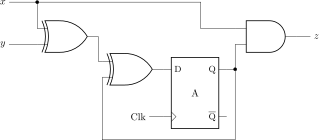
\includegraphics[width=262.3pt]{lect_8_analysis_example_fsm}\caption{circuit}\label{fig:fsm-an}
\end{subfigure}
\\[6pt]
\begin{subfigure}[b]{188.1pt}\centering
  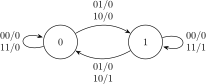
\includegraphics[width=186.1pt]{lect_8_analysis_example_state_diagram}\caption{state diagram}\label{fig:fsm-an-state}
\end{subfigure}
\caption{The circuit analysed in \cref{ex:fsm-an}.}
\end{figure}

\section{Synthesis of an FSM}\label{sec:fsm-synth}
\termx{Synthesis}{synthesis} creates a circuit from a description of behaviour.
\begin{enumerate}
  \item \textbf{Understand the specification}: inputs, outputs, initial state.
  \item Create the \textbf{state diagram}.
  \item Create the \textbf{state table}.
  \item (Optional) \textbf{state minimisation}: merge equivalent states.
  \item \textbf{State assignment}: assign binary codes to states.
  \item Choose the \textbf{flip-flop type} (D, JK, T).
  \item Derive the \textbf{logic equations} for the flip-flop inputs and outputs with K-maps.
  \item Draw the \textbf{logic diagram} and, in a modern flow, write the VHDL.
\end{enumerate}

\paragraph{State encoding.} A machine with $N$ states needs at least $\lceil\log_2N\rceil$ flip-flops. \emph{Binary} encoding uses this minimum, but the next-state logic can be complex. \emph{Gray} encoding gives adjacent states that differ in one bit, which suits counters and reduces glitches. \emph{One-hot} encoding uses $N$ flip-flops, exactly one of which is 1 in each state; it needs more flip-flops but simpler and faster logic, and is popular in FPGAs, which are rich in flip-flops. In VHDL an enumerated state type leaves the choice of encoding to the synthesis tool.

\section{Design Examples}\label{sec:fsm-examples}

\subsection{A 2-bit up/down counter}
\begin{example}{2-bit up/down counter}{updown}
Design a synchronous 2-bit counter that counts up when $x=1$ and down when $x=0$, using JK flip-flops.

\textbf{State table.} The states are 00, 01, 10, 11. For $x=1$: $00\to01\to10\to11\to00$; for $x=0$: $00\to11\to10\to01\to00$. The excitation table (\cref{tab:updown}) is obtained from the transitions of each flip-flop with the JK excitation table of \cref{tab:excit}.

\textbf{Equations.} All entries for $Q_0$ are 1 or X, so $J_0=K_0=1$ ($Q_0$ toggles on every clock). For $Q_1$ the K-maps (\cref{fig:updown-km}) give
\[
 J_1 = K_1 = x\odot Q_0 = \overline{x\xor Q_0}.
\]
Check: counting up ($x=1$), $Q_1$ must toggle when $Q_0=1$; counting down ($x=0$) it toggles when $Q_0=0$; in both cases $x\odot Q_0=1$. The circuit is \cref{fig:updown-circ}.
\end{example}

\begin{table}[htbp]
\centering
\small
\caption{Excitation table of the 2-bit up/down counter.}
\label{tab:updown}
\begin{tabular}{cc|c|cc|cccc}
\toprule
\multicolumn{2}{c|}{PS} & Input & \multicolumn{2}{c|}{NS} & $J_1$&$K_1$&$J_0$&$K_0$\\
$Q_1$&$Q_0$&$x$&$Q_1^+$&$Q_0^+$&&&&\\ \midrule
0&0&0&1&1&1&X&1&X\\0&0&1&0&1&0&X&1&X\\
0&1&0&0&0&0&X&X&1\\0&1&1&1&0&1&X&X&1\\
1&0&0&0&1&X&1&1&X\\1&0&1&1&1&X&0&1&X\\
1&1&0&1&0&X&0&X&1\\1&1&1&0&0&X&1&X&1\\ \bottomrule
\end{tabular}
\end{table}

\begin{figure}[htbp]
\centering
\begin{subfigure}[b]{346.6pt}\centering
  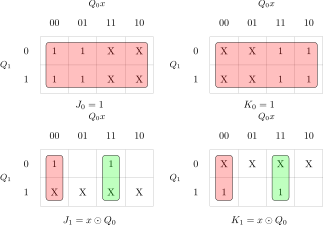
\includegraphics[width=344.6pt]{lect_8_up_down_counter_kmaps}\caption{K-maps}\label{fig:updown-km}
\end{subfigure}
\\[6pt]
\begin{subfigure}[b]{294.1pt}\centering
  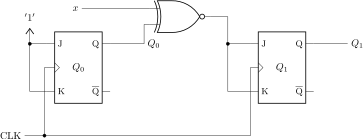
\includegraphics[width=292.1pt]{lect_8_up_down_counter_circuit}\caption{logic diagram}\label{fig:updown-circ}
\end{subfigure}
\caption{Synthesis of the 2-bit up/down counter.}
\end{figure}

\subsection{A car security system (Moore)}
\begin{example}{Car security controller}{carsec}
Design a controller with inputs $M$ (master switch), $D$ (door sensor), $V$ (vibration sensor) and output $A$ (alarm siren). The system is initially disarmed. If $M=1$ it is armed; if it is armed and a door or the vibration sensor trips, the siren sounds. Once the siren sounds it stays on until $M=0$.

\textbf{State diagram.} Two states: \emph{No\_Siren} ($Q=0$, $A=0$) and \emph{Siren} ($Q=1$, $A=1$) (\cref{fig:car-fsm}). The output depends only on the state: a Moore machine.

\textbf{State table} (\cref{tab:carsec}). The K-maps (\cref{fig:car-km}) give
\[
 Q^+ = M\,(Q + D + V),\qquad A = Q .
\]
The circuit is \cref{fig:car-circ} and \cref{lst:carsec} the VHDL.
\end{example}

\begin{table}[htbp]
\centering
\caption{State table of the car security controller.}
\label{tab:carsec}
\begin{tabular}{l|ccc|c|c}
\toprule
State $Q$ & $M$&$D$&$V$&$Q^+$&$A$\\ \midrule
0 (No\_Siren)&0&X&X&0&0\\0 (No\_Siren)&1&0&0&0&0\\0 (No\_Siren)&1&1&X&1&0\\0 (No\_Siren)&1&X&1&1&0\\
1 (Siren)&0&X&X&0&1\\1 (Siren)&1&X&X&1&1\\ \bottomrule
\end{tabular}
\end{table}

\begin{figure}[htbp]
\centering
\begin{subfigure}[b]{161.4pt}\centering
  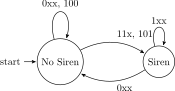
\includegraphics[width=159.4pt]{lect_8_car_security_fsm}\caption{state diagram}\label{fig:car-fsm}
\end{subfigure}
\hfill
\begin{subfigure}[b]{198.7pt}\centering
  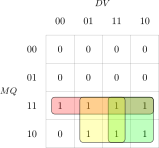
\includegraphics[width=196.7pt]{lect_8_car_security_kmaps}\caption{K-map}\label{fig:car-km}
\end{subfigure}
\\[6pt]
\begin{subfigure}[b]{262.8pt}\centering
  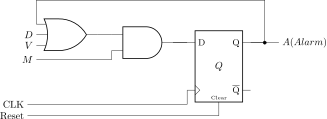
\includegraphics[width=260.8pt]{lect_8_car_security_circuit}\caption{circuit}\label{fig:car-circ}
\end{subfigure}
\caption{Car security controller.}
\end{figure}

\vhdlfile{listings/ch08_car_security.vhd}{VHDL of the car security controller: an enumerated state type, a state-register process and a combinational process (the two-process method).}{lst:carsec}

The VHDL uses an \emph{enumerated type} to give names to the states, so the designer does not have to choose binary codes by hand. It follows the \term{two-process method}: a \emph{sequential} process updates \code{current_state} on the clock edge (with an asynchronous reset), and a \emph{combinational} process computes \code{next_state} and the outputs from \code{current_state} and the inputs. Default assignments at the beginning of the combinational process (\code{next_state <= current_state;} and \code{A <= '0';}) guarantee that every signal is assigned in every path, which prevents unintended latches.

\subsection{A modulo-6 counter with enable}
\begin{example}{Modulo-6 up-counter}{mod6}
Design a synchronous counter that counts $0,1,\dots,5$ and repeats, with a count-enable input $C$ and an output $Y=1$ when the state is 5, using D flip-flops.

\textbf{State table.} States 000 to 101 (\cref{tab:mod6}); the unused states 110 and 111 are don't-cares. K-maps (\cref{fig:mod6-km}) give
\begin{align*}
 D_2 &= Q_2Q_0' + Q_2C' + Q_1Q_0C, & D_1 &= Q_1C' + Q_1Q_0' + Q_2'Q_1'Q_0C,\\
 D_0 &= Q_0\xor C, & Y &= Q_2Q_1'Q_0 .
\end{align*}
The circuit is \cref{fig:mod6-circ}. \Cref{lst:mod6} is a behavioural VHDL description of the same machine, which is much shorter than the equations: \emph{describing what the machine does} lets the tool derive the logic.
\end{example}

\begin{table}[htbp]
\centering
\caption{State table of the modulo-6 counter with enable $C$.}
\label{tab:mod6}
\begin{tabular}{ccc|ccc|ccc|c}
\toprule
\multicolumn{3}{c|}{PS} & \multicolumn{3}{c|}{NS, $C=0$} & \multicolumn{3}{c|}{NS, $C=1$} & $Y$\\ \midrule
0&0&0&0&0&0&0&0&1&0\\0&0&1&0&0&1&0&1&0&0\\0&1&0&0&1&0&0&1&1&0\\
0&1&1&0&1&1&1&0&0&0\\1&0&0&1&0&0&1&0&1&0\\1&0&1&1&0&1&0&0&0&1\\
\multicolumn{3}{c|}{1xx (110, 111)}&\multicolumn{3}{c|}{xxx}&\multicolumn{3}{c|}{xxx}&x\\ \bottomrule
\end{tabular}
\end{table}

\begin{figure}[htbp]
\centering
\begin{subfigure}[b]{252.3pt}\centering
  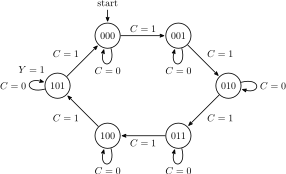
\includegraphics[width=250.3pt]{lect_8_modulo_6_counter}\caption{state diagram}
\end{subfigure}
\caption{Modulo-6 counter with enable.}
\end{figure}

\begin{figure}[htbp]
\centering
\ContinuedFloat
\begin{subfigure}[b]{356.9pt}\centering
  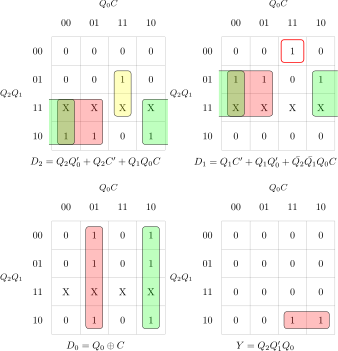
\includegraphics[width=354.9pt]{lect_8_modulo_6_kmaps}\caption{K-maps}\label{fig:mod6-km}
\end{subfigure}
\caption[]{Modulo-6 counter with enable.}
\end{figure}

\begin{figure}[htbp]
\centering
\ContinuedFloat
\begin{subfigure}[b]{412.0pt}\centering
  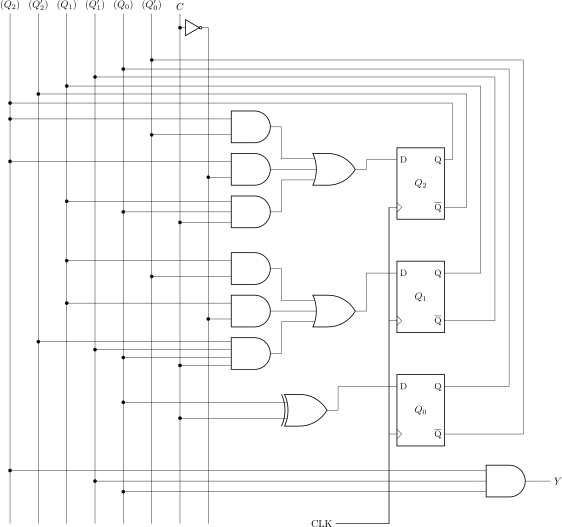
\includegraphics[width=410.0pt]{lect_8_modulo_6_circuit}\caption{logic diagram}\label{fig:mod6-circ}
\end{subfigure}
\caption[]{Modulo-6 counter with enable.}
\end{figure}

\vhdlfile{listings/ch08_modulo6_behav.vhd}{Behavioural VHDL of the modulo-6 counter with enable.}{lst:mod6}

\paragraph{Type conversions in VHDL.} \Cref{lst:mod6} adds one to a vector with the expression
\begin{center}\code{std_logic_vector(unsigned(count) + 1)}\end{center} VHDL is a strongly typed language: arithmetic is defined for the types \code{unsigned} and \code{signed} of the package \code{numeric_std}, not for \code{std_logic_vector}, so one converts explicitly (\cref{fig:conv}). Type-cast functions: \code{unsigned(slv)} and \code{signed(slv)} reinterpret a \code{std_logic_vector}; \code{std_logic_vector(u)} converts back. Integers are converted with \code{to_unsigned(int, size)} and \code{to_signed(int, size)}, and numbers with \code{to_integer(u)} or \code{to_integer(s)}. The conversions of vectors are only reinterpretations of the same bits and cost no hardware.

\figw{410.0pt}{lect_8_vhdl_type_conversion}{Conversions among \code{std_logic_vector}, \code{unsigned}, \code{signed} and \code{integer} in \code{numeric_std}.}{fig:conv}

\subsection{A one-shot circuit}\label{sec:oneshot}
\begin{example}{One-shot}{oneshot}
Design a circuit that produces an output pulse $S=1$ for \emph{exactly one clock cycle} when a push-button input $B$ is pressed, however long the button is held. (Assume the button is already debounced.)

\textbf{Mealy design.} Three states: $S_0$ waits for $B=1$; $S_1$ is the pulse state, always followed by $S_2$ on the next clock; $S_2$ waits for $B=0$ (release) and then returns to $S_0$. Encoding $S_0=00$, $S_1=01$, $S_2=10$, with the unused state 11 returning to 00 (\cref{tab:oneshot}, \cref{fig:os-fsm}), and taking the output as $S=1$ in $S_0$ when $B=1$ (the Mealy output), the K-maps (\cref{fig:os-km}) give
\[
 D_1 = Q_1'Q_0 + Q_1Q_0'B,\qquad D_0 = Q_1'Q_0'B,\qquad S = Q_1'Q_0'B .
\]
The circuit is \cref{fig:os-circ}, the response to a long press is \cref{fig:os-timing}, and \cref{lst:os-mealy} the VHDL.
\end{example}

\begin{table}[htbp]
\centering
\caption{State table of the Mealy one-shot.}
\label{tab:oneshot}
\begin{tabular}{l|c|c|c}
\toprule PS $(Q_1Q_0)$ & NS ($B=0$) & NS ($B=1$) & $S$ (with $B=1$)\\ \midrule
$S_0$ (00)&00&01&1\\ $S_1$ (01)&10&10&0\\ $S_2$ (10)&00&10&0\\ unused (11)&00&00&0\\ \bottomrule
\end{tabular}
\end{table}

\begin{sidewaysfigure}[htbp]
\centering
\begin{subfigure}[b]{244.7pt}\centering
  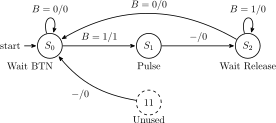
\includegraphics[width=242.7pt]{lect_8_one_shot_fsm}\caption{state diagram}\label{fig:os-fsm}
\end{subfigure}
\caption{The Mealy one-shot circuit.}
\end{sidewaysfigure}

\begin{sidewaysfigure}[htbp]
\centering
\ContinuedFloat
\begin{subfigure}[b]{499.7pt}\centering
  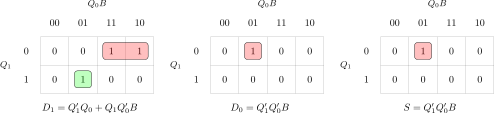
\includegraphics[width=497.7pt]{lect_8_one_shot_kmaps}\caption{K-maps}\label{fig:os-km}
\end{subfigure}
\caption[]{The Mealy one-shot circuit.}
\end{sidewaysfigure}

\begin{sidewaysfigure}[htbp]
\centering
\ContinuedFloat
\begin{subfigure}[b]{313.1pt}\centering
  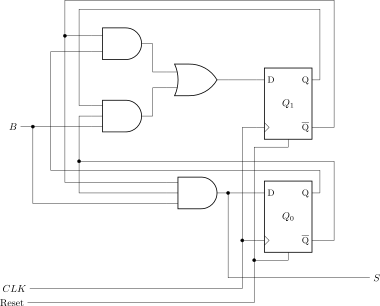
\includegraphics[width=311.1pt]{lect_8_one_shot_circuit}\caption{logic diagram}\label{fig:os-circ}
\end{subfigure}
\caption[]{The Mealy one-shot circuit.}
\end{sidewaysfigure}

\begin{sidewaysfigure}[htbp]
\centering
\ContinuedFloat
\begin{subfigure}[b]{463.4pt}\centering
  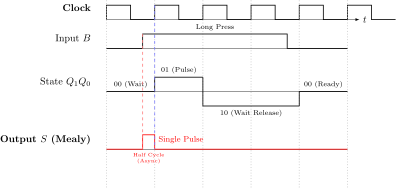
\includegraphics[width=461.4pt]{lect_8_one_shot_timing}\caption{response to a long press}\label{fig:os-timing}
\end{subfigure}
\caption[]{The Mealy one-shot circuit.}
\end{sidewaysfigure}

\vhdlfile{listings/ch08_oneshot_mealy.vhd}{VHDL of the Mealy one-shot.}{lst:os-mealy}

\paragraph{A problem with the Mealy design.} Because $S=Q_1'Q_0'B$ depends directly on the input $B$, which is not synchronised with the clock, the pulse starts when the button is pressed and ends at the next clock edge; its width is therefore \emph{less than one clock period} and varies with the moment of pressing (and any noise on $B$ passes straight to $S$). A \textbf{Moore} design solves the problem: the machine has states $S_0$ (idle, output 0, wait for $B=1$), $S_1$ (pulse, output 1, unconditionally to $S_2$) and $S_2$ (wait for $B=0$), and the output $S=1$ only in the state $S_1$. Since states change only at clock edges, the pulse starts and ends at clock edges and lasts \emph{exactly one period} (\cref{fig:os-moore,fig:os-comp}, \cref{lst:os-moore}). The price is a delay of one clock period between the press and the pulse.

\begin{figure}[htbp]
\centering
\begin{subfigure}[b]{182.9pt}\centering
  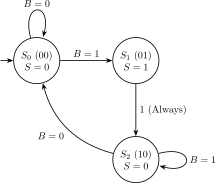
\includegraphics[width=180.9pt]{lect_8_one_shot_moore_fsm}\caption{Moore state diagram}\label{fig:os-moore}
\end{subfigure}
\\[6pt]
\begin{subfigure}[b]{412.0pt}\centering
  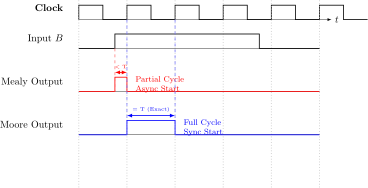
\includegraphics[width=410.0pt]{lect_8_one_shot_comparison}\caption{Mealy (asynchronous) and Moore (synchronous) pulse}\label{fig:os-comp}
\end{subfigure}
\caption{The Moore one-shot and the comparison of the two outputs.}
\end{figure}

\vhdlfile{listings/ch08_oneshot_moore.vhd}{VHDL of the Moore one-shot (exact one-cycle pulse).}{lst:os-moore}

\paragraph{VHDL coding of Moore and Mealy machines.} The two styles differ in a recognisable way, summarised in \cref{tab:vhdl-style}. In a Moore machine the outputs are assigned depending on \code{current_state} only; in a Mealy machine the output assignments are inside the \code{if} statements that test the inputs, so the process must be sensitive to the inputs as well.

\begin{table}[htbp]
\centering
\small
\caption{VHDL coding differences between Moore and Mealy machines.}
\label{tab:vhdl-style}
\begin{tabularx}{\linewidth}{@{}lXX@{}}
\toprule
 & \textbf{Moore} & \textbf{Mealy}\\ \midrule
Sensitivity list & \code{process(current_state)} (and the inputs for the next-state logic) & \code{process(current_state, inputs)}\\
Output assignment & outside any test of inputs within the \code{case} branch: \code{when S0 => A <= '1'; next_state <= S1;} & inside \code{if}/\code{case} tests of inputs: \code{when S0 => if X='1' then A<='1'; else A<='0'; end if;}\\
Timing & output stable between clock edges (comes from the state register) & output may change whenever an input changes\\ \bottomrule
\end{tabularx}
\end{table}

\subsection{A control unit}
\begin{example}{A simple processor control unit}{cpu}
An FSM is also the form of the \emph{control unit} of a processor (\cref{ch:dedicated}): it steps through the actions of a computation in response to status signals. The machine in \cref{fig:cpu-fsm} has states $s_0,\dots,s_3$ and outputs $x$ and $y$; the transitions out of $s_0$ depend on the input \textit{Start} ($Start$ and $Start'$), and those out of $s_2$ on the status signal $n=9$ ($n=9$ and $(n=9)'$). The remaining transitions are unconditional. Such a machine is synthesised exactly as the others in this chapter; note that its inputs are \emph{comparisons} produced by other circuits, a feature that we exploit in \cref{ch:dedicated,ch:gp}.
\end{example}

\figw{234.5pt}{lect_8_simple_cpu_fsm_example}{State diagram of the control unit of \cref{ex:cpu}.}{fig:cpu-fsm}

\subsection{An elevator controller: Moore and Mealy}
\begin{example}{Two-floor elevator controller (Moore)}{elev-moore}
Design the FSM for an elevator serving two floors (\cref{fig:elev-setup}). Inputs: $f_1,f_2$ are the call buttons for floors 1 and 2 (hall and cabin buttons combined, assumed to stay pressed until served) and $at_1,at_2$ are position sensors, asserted when the cabin is at floor 1 or 2. Outputs: $go_1$ (motor on) and $go_0$ (direction, $0$ = down, $1$ = up), and the floor indicators $led_1$ and $led_2$.

\textbf{State diagram} (\cref{fig:elev-moore}). Four states: \textbf{00} floor 1 (idle; $led_1$ on; on $f_2$ go to 11); \textbf{11} moving up ($go_1=go_0=1$; on $at_2$ go to 10); \textbf{10} floor 2 (idle; $led_2$ on; on $f_1$ go to 01); \textbf{01} moving down ($go_1=1,go_0=0$; on $at_1$ go to 00). The motor outputs depend on the state only, so this is a Moore machine.

\textbf{Equations.} From the K-maps of \cref{fig:elev-moore-km},
\begin{align*}
 D_1 &= Q_1'Q_0'f_2 + Q_1Q_0 + Q_1Q_0'f_1',\\
 D_0 &= Q_1'Q_0'f_2 + Q_1Q_0\,at_2' + Q_1Q_0'f_1 + Q_1'Q_0\,at_1' .
\end{align*}
Each term describes one transition: for example $Q_1Q_0\,at_2'$ keeps $D_0=1$ while the cabin moves up and has not yet arrived. \Cref{lst:elev-moore} is the VHDL.
\end{example}

\begin{figure}[htbp]
\centering
\begin{subfigure}[b]{338.4pt}\centering
  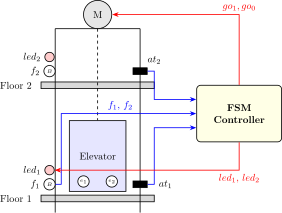
\includegraphics[width=336.4pt]{lect_8_elevator_setup}\caption{system}\label{fig:elev-setup}
\end{subfigure}
\caption{Two-floor elevator controller, Moore version.}
\end{figure}

\begin{figure}[htbp]
\centering
\ContinuedFloat
\begin{subfigure}[b]{282.0pt}\centering
  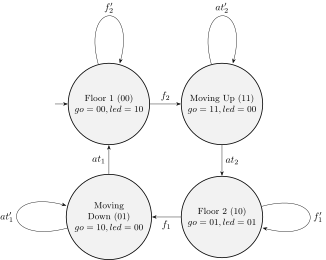
\includegraphics[width=280.0pt]{lect_8_elevator_fsm}\caption{Moore state diagram}\label{fig:elev-moore}
\end{subfigure}
\\[6pt]
\begin{subfigure}[b]{252.3pt}\centering
  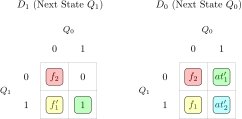
\includegraphics[width=250.3pt]{lect_8_elevator_moore_kmaps}\caption{K-maps for $D_1$, $D_0$}\label{fig:elev-moore-km}
\end{subfigure}
\caption[]{Two-floor elevator controller, Moore version.}
\end{figure}

\vhdlfile{listings/ch08_elevator_moore.vhd}{VHDL of the Moore elevator controller (four states).}{lst:elev-moore}

\begin{example}{Two-floor elevator controller (Mealy)}{elev-mealy}
The same controller can be built with only \emph{two} states, \textit{Floor1} and \textit{Floor2}, if the motor outputs are allowed to depend on the buttons. The state changes only when the cabin \emph{arrives} at a floor ($at_x$); the motor is turned on by the call button of the \emph{other} floor (\cref{fig:elev-mealy}):
\begin{align*}
 D &= \NOT{Q}\,(f_2\cdot at_2) + Q\,\overline{(f_1\cdot at_1)},\\
 led_1 &= \NOT{Q},\quad led_2 = Q,\quad go_1 = \NOT{Q}f_2 + Qf_1,\quad go_0 = \NOT{Q}.
\end{align*}
With $Q=0$ (floor 1) and $f_2$ pressed the motor runs upwards until $at_2$ arrives; the K-maps are \cref{fig:elev-mealy-km} and the VHDL \cref{lst:elev-mealy}. The state memory shrinks from two flip-flops to one, but the output logic becomes more complex, and the outputs now respond directly to the buttons. In this version the indicators show the last floor served, not the cabin position while it moves.
\end{example}

\begin{figure}[htbp]
\centering
\begin{subfigure}[b]{202.1pt}\centering
  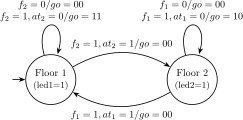
\includegraphics[width=200.1pt]{lect_8_elevator_mealy_fsm}\caption{Mealy state diagram}\label{fig:elev-mealy}
\end{subfigure}
\\[6pt]
\begin{subfigure}[b]{228.7pt}\centering
  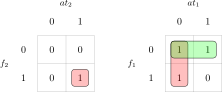
\includegraphics[width=226.7pt]{lect_8_elevator_mealy_kmaps}\caption{K-maps}\label{fig:elev-mealy-km}
\end{subfigure}
\caption{Two-floor elevator controller, Mealy version.}
\end{figure}

\vhdlfile{listings/ch08_elevator_mealy.vhd}{VHDL of the Mealy elevator controller (two states).}{lst:elev-mealy}

\section{Moore versus Mealy Timing}\label{sec:moore-mealy}
The essential difference is the timing of the outputs (\cref{fig:mm-timing}). A Moore output changes only just after a clock edge, because it is a function of the state register, so it is synchronous and stable for the whole period. A Mealy output can change at any time during the period when an input changes: it \emph{reacts one clock period earlier} than the equivalent Moore output, but it can also show glitches if the inputs change at different times, and in a chain of Mealy machines such combinational paths from input to output add up. The elevator timing diagram, \cref{fig:elev-timing}, shows a complete trip with the two versions.

\begin{sidewaysfigure}[htbp]
\centering
\begin{subfigure}[b]{544.8pt}\centering
  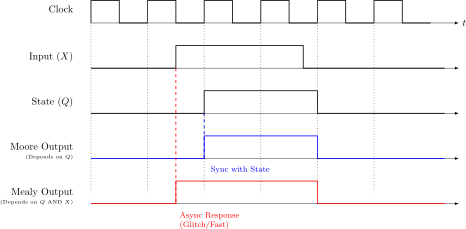
\includegraphics[width=542.8pt]{lect_8_moore_vs_mealy_timing}\caption{generic timing comparison}\label{fig:mm-timing}
\end{subfigure}
\caption{Moore and Mealy output timing.}
\end{sidewaysfigure}

\begin{sidewaysfigure}[htbp]
\centering
\ContinuedFloat
\begin{subfigure}[b]{602.0pt}\centering
  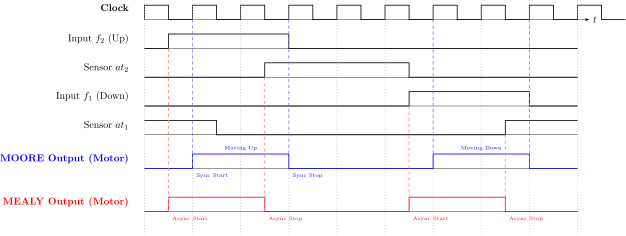
\includegraphics[width=600.0pt]{lect_8_elevator_timing}\caption{elevator, up and down}\label{fig:elev-timing}
\end{subfigure}
\caption[]{Moore and Mealy output timing.}
\end{sidewaysfigure}

\begin{keypoint}[Choosing between Moore and Mealy]
Use a \textbf{Moore} machine when the outputs must be glitch-free and aligned with the clock, or drive other synchronous logic (the usual choice). Use a \textbf{Mealy} machine when you need the fastest reaction or the smallest number of states, and take care that the inputs are synchronised. Any Mealy machine has an equivalent Moore machine, usually with more states.
\end{keypoint}

\section{Timing of a Synchronous FSM}\label{sec:fsm-timing}
All state changes occur at the active clock edge, but the next state must be \emph{ready} before the next edge. The signal path is: clock edge $\to$ flip-flop output ($t_{pcq}$, the propagation delay from clock to $Q$) $\to$ next-state logic ($t_{comb}$) $\to$ flip-flop input, which must be stable for the \emph{setup time} $t_{setup}$ before the next edge. Hence
\begin{equation}
  T_{clk} \;\ge\; t_{pcq} + t_{comb} + t_{setup},\qquad f_{max}=\frac{1}{t_{pcq}+t_{comb}+t_{setup}} .
  \label{eq:fmax}
\end{equation}
If $t_{pcq}=0.5$~ns, $t_{comb}=3$~ns and $t_{setup}=0.2$~ns, then $T_{clk}\ge3.7$~ns and $f_{max}\approx270$~MHz. In addition the inputs must remain stable for the \emph{hold time} $t_{hold}$ after the edge. Equation~\eqref{eq:fmax} explains why a design with more complex next-state logic (a longer $t_{comb}$) must run slower, and why one-hot encoding, with its simpler logic, is often faster.

\section{A Template for VHDL State Machines}
Most FSMs in this book follow one template.

\begin{lstlisting}[caption={Template of the two-process FSM description (the state register is process 1 and the combinational logic process 2).},label={lst:fsm-template}]
architecture fsm of my_machine is
  type state_type is (S0, S1, S2);                  -- list the states
  signal current_state, next_state : state_type;
begin
  -- Process 1: state register (sequential)
  process (clk, reset)
  begin
    if reset = '1' then
      current_state <= S0;                          -- initial state
    elsif rising_edge(clk) then
      current_state <= next_state;
    end if;
  end process;

  -- Process 2: next-state and output logic (combinational)
  process (current_state, x)                        -- all signals that are read
  begin
    next_state <= current_state;                    -- defaults: stay, outputs inactive
    y <= '0';
    case current_state is
      when S0 => if x = '1' then next_state <= S1; end if;
      when S1 => y <= '1'; next_state <= S2;        -- Moore output
      when S2 => if x = '0' then next_state <= S0; end if;
    end case;
  end process;
end fsm;
\end{lstlisting}

A common error is to omit a signal from the sensitivity list: for example, writing \code{process(clk)} for the register above without \code{reset} makes the asynchronous reset ineffective in simulation. In process 2 the sensitivity list must contain \emph{every signal that is read}.

\begin{chaptersummary}
\begin{itemize}
  \item An \textbf{FSM} has next-state logic, a state register and output logic. \textbf{Moore}: output = $f$(state). \textbf{Mealy}: output = $f$(state, inputs).
  \item \textbf{Analysis}: equations $\to$ state table $\to$ state diagram. \textbf{Synthesis}: specification $\to$ state diagram $\to$ state table $\to$ (minimisation) $\to$ state assignment $\to$ flip-flop type $\to$ K-maps $\to$ logic diagram or VHDL.
  \item \textbf{State encodings}: binary (fewest flip-flops), Gray, one-hot ($N$ flip-flops, simpler logic).
  \item In VHDL use an \textbf{enumerated state type} and the \textbf{two-process method}; assign defaults to avoid latches; use \code{numeric_std} and explicit conversions for arithmetic.
  \item The \textbf{one-shot} shows the difference between the models: the Mealy output is asynchronous (less than one clock), the Moore output is exactly one cycle but delayed.
  \item The clock period must satisfy $T_{clk}\ge t_{pcq}+t_{comb}+t_{setup}$.
\end{itemize}
\end{chaptersummary}

\chapsec{Exercises}
\begin{exlist}
  \item \textbf{Moore or Mealy?} Machine (A) has next-state logic with inputs \{inputs, present state\} and output logic with inputs \{present state\}. Machine (B) has output logic with inputs \{inputs, present state\}. Which is Moore and which is Mealy?
  \item \textbf{State analysis.} A state machine has one JK flip-flop with $J=x$ and $K=1$. If the present state is $Q=0$ and $x=1$, what is the next state? Give the complete state table.
  \item \textbf{110 detector, overlapping.} Draw the state diagram of a Mealy sequence detector for the sequence \texttt{110} in which overlapping sequences are valid. For the input \texttt{0 1 1 0 1 1 0} the output must be \texttt{0 0 0 1 0 0 1}.
  \item \textbf{110 detector, non-overlapping.} Draw the state diagram of a \emph{non-overlapping} detector for \texttt{110}: after a detection the machine returns to the initial state. Explain why the two diagrams are the same for the sequence \texttt{110} but would differ for \texttt{101}.
  \item \textbf{State encoding.} An FSM has 12 states. How many flip-flops are needed with (a)~binary encoding; (b)~one-hot encoding?
  \item \textbf{VHDL syntax.} What is missing in the sensitivity list of this synchronous-FSM state-register process? \begin{lstlisting}
process (clk)
begin
  if reset = '1' then current_state <= S0;
  elsif rising_edge(clk) then current_state <= next_state;
  end if;
end process;
\end{lstlisting}
  \item \textbf{State-table construction.} Counter sequence $00\to01\to10\to11\to00$ with an input that is 0 for hold and 1 for count. Give the missing next state for present state $01$ and input 1.
  \item \textbf{Logic equation.} In the K-map of \cref{fig:ex88} for $D_0$ (rows $Q$, columns $X$), derive the simplified Boolean equation.
  \item \textbf{Timing.} Which of the following correctly bounds the clock period of an FSM? (1)~$T_{clk}\ge t_{setup}+t_{hold}$; (2)~$T_{clk}\ge t_{pcq}+t_{comb}+t_{setup}$; (3)~$T_{clk}\ge t_{pcq}+t_{comb}-t_{hold}$. Compute $f_{max}$ if $t_{pcq}=0.4$~ns, $t_{comb}=2.1$~ns and $t_{setup}=0.3$~ns.
  \item \textbf{Gray-code counter.} Design a 2-bit Gray-code counter with the sequence $00\to01\to11\to10\to00$: draw the state diagram, find the D flip-flop equations and the circuit.
  \item Convert the Mealy 101 detector of \cref{ex:seqdet} to a \emph{Moore} machine. How many states are needed? Draw the state diagram.
  \item Design a Moore FSM for a simple traffic light with states Green, Yellow and Red, which changes state on every clock pulse when an input \code{tick} is 1. Give the state diagram, a binary state assignment, the equations and VHDL.
  \item Write the VHDL of a Moore machine whose output $z$ is 1 while the input $x$ has been 1 for at least three consecutive clock cycles.
  \item Explain, with a sketch, why the output of a Mealy machine can show a glitch when two inputs change at slightly different times, and why a Moore output cannot.
  \item For the Mealy one-shot, draw the waveforms of $B$, the clock and $S$ if $B$ rises between two clock edges and falls after three clock periods. Compare with the Moore version.
\end{exlist}

\begin{figure}[htbp]
\centering
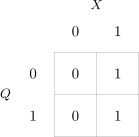
\includegraphics[width=129pt]{lect_8_exercise_8_8_kmap}
\caption{K-map for Exercise~8.8.}
\label{fig:ex88}
\end{figure}

\chapsec{Further Reading}
Mealy's and Moore's original papers~\cite{mealy1955,moore1956} introduced the two models. The synthesis of FSMs and their VHDL descriptions are treated in Chapter~8 of Brown and Vranesic~\cite{brown2009} and Chapter~5 of Hwang~\cite{hwang2005}; the coding templates for state machines follow Ashenden~\cite{ashenden2008}. Gajski~\cite{gajski1997} extends FSMs with a datapath, the topic of the next chapter.

\chapter{Dedicated Microprocessors}\label{ch:dedicated}

\begin{objectives}
After studying this chapter you will be able to:
\begin{itemize}
  \item describe the von Neumann model of a computer and the layers of abstraction from transistors to processors;
  \item explain what a dedicated microprocessor is and how it divides into a \emph{datapath} and a \emph{control unit};
  \item describe computations at the register-transfer level (RTL);
  \item design a datapath for a given algorithm and write its \emph{control words};
  \item design the control unit as an FSM driven by status signals, including a wait state when needed for timing;
  \item implement a dedicated processor in VHDL in the FSM+D style and in the FSMD style.
\end{itemize}
\end{objectives}

\section{The Von Neumann Model}\label{sec:vonneumann}
Almost every computer follows the model described by John von Neumann in 1945~\cite{vonneumann1945}. It has five components (\cref{fig:vn}): \textbf{input} supplies data, \textbf{output} presents results, \textbf{memory} stores programs and data, and the \textbf{microprocessor} (the ``brain'') processes the data. The microprocessor has a \textbf{datapath}, which carries out the data processing (arithmetic and logic), and a \textbf{control unit}, which determines the sequence of operations.

\figw{301.8pt}{lect_9_von_neumann_model}{The von Neumann model of a computer.}{fig:vn}

\section{From Transistors to Microprocessors}
Digital systems are so complex that they can only be designed by managing complexity through \emph{layers of abstraction} (\cref{fig:hier}). Transistors combine into logic gates; gates form combinational and sequential circuits; circuits form functional components such as adders and multiplexers (Chapters~4 and~5) and registers and counters (Chapter~7); and components are integrated into a datapath and a control unit, which together form the microprocessor. Each layer hides the details of the layer below it, so a designer can work at the level of components without thinking of transistors. This chapter works at the top two layers.

\figw{243.9pt}{lect_9_digital_hierarchy}{Layers of abstraction: from transistors to microprocessors.}{fig:hier}

\section{Dedicated Microprocessors}
A \term{dedicated microprocessor} (special-purpose processor) is designed to perform one specific task. The ``program'' is not stored in memory but is \emph{hardwired} in the structure of the processor, which makes it optimised for the task in speed, power and size. Its function cannot be changed after manufacture (if implemented as an ASIC; an FPGA implementation can be reconfigured). Examples are the image-processing chip in a digital camera, the controller in a microwave oven and a GCD engine inside a cryptographic circuit. In contrast, a \emph{general-purpose} processor executes arbitrary programs stored in memory and is the subject of \cref{ch:gp}.

\section{Datapath and Control Unit}\label{sec:dpcu}
A microprocessor is partitioned into two cooperating parts (\cref{fig:dpcu}).
\begin{itemize}
  \item The \term{datapath} performs the data processing operations. It contains functional units (ALUs, adders, comparators), registers, counters and multiplexers; this is where the ``number crunching'' happens.
  \item The \term{control unit} determines the \emph{sequence} of datapath operations. In each clock cycle it generates \term{control signals}, which tell the datapath what to do (load this register, select that input), and it receives \term{status signals} from the datapath (the result is zero, $A>B$) which it uses to make decisions. The control unit is an FSM, as studied in \cref{ch:fsm}.
\end{itemize}

\figw{261.1pt}{lect_9_datapath_control}{A dedicated microprocessor: the control unit sends control signals to the datapath and receives status signals from it.}{fig:dpcu}

\section{Register Transfer Level}\label{sec:rtl}
The \term{register-transfer level} (RTL) is the level of abstraction at which a synchronous digital system is described by (1)~the flow of data between registers and (2)~the logical or arithmetic operations performed on the data on the way (\cref{fig:rtl}). At RTL we consider information moving ``in bulk'' from register to register at each clock tick, ignoring the gates and flip-flops that implement it. This is the level of abstraction of VHDL and Verilog, and of the notation $R_1\leftarrow R_2+R_3$ used in this chapter, meaning ``at the next active clock edge, load $R_1$ with the sum of the contents of $R_2$ and $R_3$''.

\figw{298.3pt}{lect_9_rtl_model}{The RTL model: registers, combinational logic between them, and a common clock.}{fig:rtl}

\section{Datapath Design}\label{sec:datapath}
To design a datapath for a single problem, assemble the registers and functional units needed to perform the required operations, then connect them so that every transfer in the algorithm has a path.

\begin{example}{Datapath for $A=B+C$}{dp1}
Registers $B$ and $C$ hold the operands; an adder forms $B+C$; register $A$ stores the result when the control signal $ALoad$ is asserted (\cref{fig:dp-abc}).
\end{example}

\begin{example}{Datapath for $A=A+3$}{dp2}
The output of register $A$ is fed back to one input of an adder; the other input is the constant 3; the sum is loaded back into $A$ (\cref{fig:dp-a3}). The control unit asserts $ALoad$ once for each addition.
\end{example}

\begin{figure}[htbp]
\centering
\begin{subfigure}[b]{313.3pt}\centering
  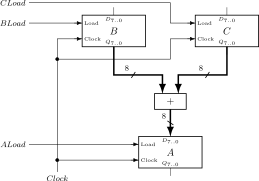
\includegraphics[width=311.3pt]{lect_9_datapath_A_B_plus_C}\caption{$A=B+C$}\label{fig:dp-abc}
\end{subfigure}
\\[6pt]
\begin{subfigure}[b]{198.6pt}\centering
  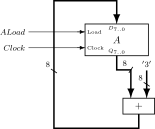
\includegraphics[width=196.6pt]{lect_9_datapath_A_plus_3}\caption{$A=A+3$}\label{fig:dp-a3}
\end{subfigure}
\caption{Two dedicated datapaths.}
\end{figure}

\subsection{Sharing a functional unit with multiplexers}
Suppose the processor must perform \emph{both} $A=A+3$ and $A=B+C$. Two adders would work, but a single adder preceded by multiplexers is cheaper. A multiplexer in front of each adder input selects the operand: the first chooses between $B$ ($0$) and $A$ ($1$), the second between $C$ ($0$) and the constant $3$ ($1$) (\cref{fig:dp-shared}). Because the two operations need either $(B,C)$ or $(A,3)$, one control signal $\mathit{Mux}$ can drive both multiplexers. The control unit selects the operation by the \emph{control word}, i.e.\ the values of all control signals needed in a clock cycle (\cref{tab:cw1}).

\figw{392.6pt}{lect_9_datapath_one_adder}{A shared-adder datapath that performs $A=A+3$ and $A=B+C$. Both multiplexers are driven by the same control signal $Mux$ (input $1$ selects $A$ and the constant $3$, input $0$ selects $B$ and $C$); the bus width is marked with a slash, and the clock is common to all registers.}{fig:dp-shared}

The two multiplexers can also be placed \emph{in front of the destination register} instead: the adder outputs $B+C$ and $A+3$ feed a single 2-to-1 multiplexer $Amux$ that selects what is loaded into $A$ (\cref{fig:dp-combine}). This version needs two adders but only one multiplexer, and the same $ALoad$ and $Amux$ signals again define the two operations.

\figw{265.0pt}{lect_9_datapath_combine}{Alternative datapath for $A=B+C$ and $A=A+3$: one multiplexer $Amux$ in front of register $A$.}{fig:dp-combine}

\begin{table}[htbp]
\centering
\caption{Control words of the shared-adder datapath.}
\label{tab:cw1}
\begin{tabular}{l|cc}
\toprule Operation & $ALoad$ & $Mux$\\ \midrule
$A=A+3$ & 1 & 1\\ $A=B+C$ & 1 & 0\\ \bottomrule
\end{tabular}
\end{table}

\subsection{Status signals and conditional operations}
To implement a conditional such as \textbf{IF} $(A=0)$ the datapath must produce a \emph{status signal} for the control unit. An equality comparator can compare a register with a constant (\cref{fig:dp-if}a). For $A=0$ in an 8-bit register there is a cheaper solution: a single 8-input NOR gate, whose output is 1 only if every bit of $A$ is 0 (\cref{fig:dp-if}b). Similarly, a magnitude comparator (\cref{sec:comparator}) produces $A>B$.

\figw{332.0pt}{lect_9_datapath_if}{Generating the status signal $(A=0)$: (a)~comparator with the constant $0$; (b)~8-input NOR gate.}{fig:dp-if}

\subsection{An if-then-else datapath}
Consider the algorithm
\begin{center}\ttfamily\small
INPUT A;\quad IF (A = 5) THEN B = 8 ELSE B = 13; \quad OUTPUT B
\end{center}
The datapath of \cref{fig:ite-dp} has register $A$ (the input), register $B$ (the result), a multiplexer selecting the constant 8 or 13, an AND gate that generates the status signal $(A=5)$ by decoding the bit pattern $0101$ (the inputs for $A_3$ and $A_1$ are inverted), and an output buffer controlled by $Out$. The control signals are $ALoad$, $BLoad$, $Muxsel$ ($1$ selects 8, $0$ selects 13) and $Out$. The algorithm is converted into a sequence of control words (\cref{tab:cw-ite}); the control unit decides between control words 2 and 3 using the status signal $(A=5)$.

\figw{282.1pt}{lect_9_datapath_if_then_else}{Datapath for the if-then-else algorithm.}{fig:ite-dp}

\begin{table}[htbp]
\centering
\caption{Control words for the if-then-else algorithm.}
\label{tab:cw-ite}
\begin{tabular}{cl|cccc}
\toprule CW & Instruction & $ALoad$ & $Muxsel$ & $BLoad$ & $Out$\\ \midrule
1 & INPUT A & 1 & X & 0 & 0\\ 2 & $B=8$ & 0 & 1 & 1 & 0\\ 3 & $B=13$ & 0 & 0 & 1 & 0\\ 4 & OUTPUT B & 0 & X & 0 & 1\\ \bottomrule
\end{tabular}
\end{table}

\subsection{A datapath with a loop: summing the numbers 1 to 10}
\begin{center}\ttfamily\small
\begin{tabular}{@{}l@{}}
Sum = 0\\ i = 1\\ DO \{\\ \quad Sum = Sum + i\\ \quad i = i + 1\\ \} WHILE (i != 11)\\ OUTPUT Sum
\end{tabular}
\end{center}
The datapath needs two registers, $Sum$ and $i$, an adder, and a gate that signals when $i\neq11$. We build it (\cref{fig:sum-dp}) with \emph{one} adder, whose first input is always $i$ and whose second input is chosen by $\mathit{addMux}$: $Sum$ (0) or the constant 1 (1). The adder output $R$ goes to both registers through input multiplexers: $\mathit{sumMux}$ chooses between $R$ (0) and the constant 0 (1), and $\mathit{iMux}$ between $R$ (0) and the constant 1 (1). With these selections each instruction of the algorithm is one control word (\cref{tab:cw-sum}): $Sum=0$ is $sumLoad=1$, $sumMux=1$; $i=1$ is $iLoad=1$, $iMux=1$; $Sum=Sum+i$ is $sumLoad=1$, $sumMux=0$, $addMux=0$; $i=i+1$ is $iLoad=1$, $iMux=0$, $addMux=1$; and the output is $OE=1$. The loop is made by the control unit (\cref{sec:cu-design}).

\figw{370.5pt}{lect_9_datapath_sum_1_to_10}{A datapath for summing the numbers from 1 to 10 with one adder and three multiplexers. The status signal $(i\neq11)$ is a NAND gate whose inputs for the zero bits of $11=00001011_2$ are inverted; the output $Sum$ is enabled by $OE$.}{fig:sum-dp}

\begin{table}[htbp]
\centering
\caption{Control words for the summation algorithm.}
\label{tab:cw-sum}
\begin{tabular}{cl|cccccc}
\toprule CW & Instruction & $sumLoad$ & $sumMux$ & $iLoad$ & $iMux$ & $addMux$ & $OE$\\ \midrule
1 & $Sum=0$ & 1 & 1 & 0 & X & X & 0\\
2 & $i=1$ & 0 & X & 1 & 1 & X & 0\\
3 & $Sum=Sum+i$ & 1 & 0 & 0 & X & 0 & 0\\
4 & $i=i+1$ & 0 & X & 1 & 0 & 1 & 0\\
5 & OUTPUT $Sum$ & 0 & X & 0 & X & X & 1\\ \bottomrule
\end{tabular}
\end{table}

\section{Control Unit Design}\label{sec:cu-design}
The control unit is an FSM (\cref{fig:dpcu}) that steps through the control words of the algorithm and branches on the status signals. In a Moore machine, each state outputs one control word. We design three control units.

\subsection{Example 1: counting from 1 to 10}
\begin{example}{Counter control unit}{cu1}
The algorithm is \texttt{i = 0; WHILE (i != 10) \{ i = i + 1 \}}. The datapath is a counter $i$ with a clear input and a count input and a comparator producing the status signal $(i=10)$ (\cref{fig:cnt-dp}). The control signals are \emph{Clear} and \emph{Count}.

\textbf{State diagram} (\cref{fig:cnt-fsm}). $S_0$: clear the counter. $S_1$: increment; remain in $S_1$ while $i\neq10$ and leave when $i=10$. $S_2$: the loop is finished. A fourth state $S_3$ (halt) keeps the machine idle after the computation. With the state assignment $S_0=00$, $S_1=01$, $S_2=10$, $S_3=11$ and $x$ denoting the status signal $(i=10)$, the next-state table (\cref{tab:cu1}) and the Moore output table give
\begin{align*}
 D_1 &= Q_1 + Q_0x, & D_0 &= Q_1 + Q_0' + x',\\
 Clear &= Q_1'Q_0' = \overline{Q_1+Q_0}, & Count &= Q_1'Q_0 .
\end{align*}
The control logic is \cref{fig:cnt-logic}; connected to the datapath it forms the complete dedicated microprocessor of \cref{fig:cnt-comb}.
\end{example}

\begin{table}[htbp]
\centering
\caption{Tables of the counter control unit ($x=(i=10)$).}
\label{tab:cu1}
\begin{tabular}{cc|cc}
\toprule PS $Q_1Q_0$ & Input $x$ & NS $D_1D_0$ & \\ \midrule
00 ($S_0$)&X&01 ($S_1$)&\\ 01 ($S_1$)&0&01 ($S_1$)&\\ 01 ($S_1$)&1&10 ($S_2$)&\\
10 ($S_2$)&X&11 ($S_3$)&\\ 11 ($S_3$)&X&11 ($S_3$)&\\ \bottomrule
\end{tabular}\qquad
\begin{tabular}{c|cc}
\toprule State & Clear & Count\\ \midrule
00 ($S_0$)&1&0\\01 ($S_1$)&0&1\\10 ($S_2$)&0&0\\11 ($S_3$)&0&0\\ \bottomrule
\end{tabular}
\end{table}

\begin{figure}[htbp]
\centering
\begin{subfigure}[b]{174.9pt}\centering
  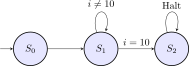
\includegraphics[width=172.9pt]{lect_9_counter_fsm}\caption{control FSM}\label{fig:cnt-fsm}
\end{subfigure}
\hfill
\begin{subfigure}[b]{202.6pt}\centering
  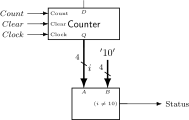
\includegraphics[width=200.6pt]{lect_9_counter_datapath}\caption{datapath}\label{fig:cnt-dp}
\end{subfigure}
\\[6pt]
\begin{subfigure}[b]{300.0pt}\centering
  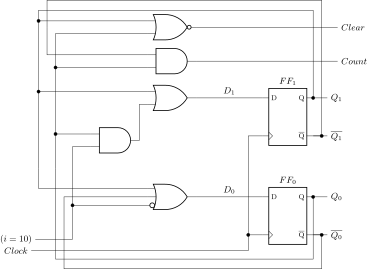
\includegraphics[width=298.0pt]{lect_9_counter_logic}\caption{control logic}\label{fig:cnt-logic}
\end{subfigure}
\caption{The counter processor of \cref{ex:cu1}.}
\end{figure}

\begin{figure}[htbp]
\centering
\ContinuedFloat
\begin{subfigure}[b]{409.4pt}\centering
  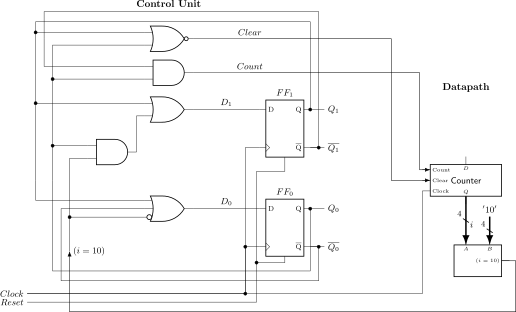
\includegraphics[width=407.4pt]{lect_9_counter_combined}\caption{complete processor}\label{fig:cnt-comb}
\end{subfigure}
\caption[]{The counter processor of \cref{ex:cu1}.}
\end{figure}

\subsection{Example 2: the if-then-else control unit}
\begin{example}{if-then-else control unit}{cu2}
The control signals and control words are those of \cref{tab:cw-ite}; the status signal is $(A=5)$. A first design has the states $S_{input}$ (load $A$), $S_{equal}$ ($B=8$), $S_{notequal}$ ($B=13$) and $S_{output}$, with $S_{input}$ branching directly on the status signal (\cref{fig:ite-fsm-noextra}).

\textbf{The timing problem.} In $S_{input}$ register $A$ is loaded \emph{at the end of the clock cycle}. The control unit takes its branching decision at the same clock edge, so it sees the status signal computed from the \emph{old} contents of $A$ and may go to the wrong state. The simulation of \cref{fig:ite-nowait} shows this error. The remedy is an extra \textbf{wait state} $S_{extra}$ after $S_{input}$, in which nothing happens for one clock period: register $A$ takes its new value and the comparator settles, and the next state is decided in $S_{extra}$ using the correct status (\cref{fig:ite-fsm,fig:ite-wait}).

\textbf{Synthesis.} With the state assignment $S_{input}=000$, $S_{extra}=001$, $S_{notequal}=010$, $S_{equal}=011$, $S_{output}=100$ the next-state table is \cref{tab:ite-ns}. Writing $I$ for the status signal $(A=5)$:
\begin{align*}
 D_2 &= Q_2+Q_1, & D_1 &= Q_1'Q_0, & D_0 &= Q_2'Q_1'(Q_0'+I),\\
 ALoad &= Q_2'Q_1'Q_0', & BLoad &= Q_2'Q_1, & Muxsel &= Q_0, & Out &= Q_2 .
\end{align*}
Muxsel is 1 in $S_{equal}$ (select 8) and 0 in $S_{notequal}$ (select 13); in $S_{extra}$ it is a don't-care. The VHDL is \cref{lst:ite-cu}, in which the state register is built of D flip-flops and the logic is written as the equations above, and \cref{fig:ite-comb} shows the control unit connected to the datapath.
\end{example}

\begin{table}[htbp]
\centering
\caption{Next-state and output tables of the if-then-else control unit with wait state ($I=(A=5)$).}
\label{tab:ite-ns}
\begin{tabular}{cc|c}
\toprule Present state & $I$ & Next state\\ \midrule
000 ($S_{input}$)&X&001\\ 001 ($S_{extra}$)&0&010\\ 001 ($S_{extra}$)&1&011\\
010 ($S_{notequal}$)&X&100\\ 011 ($S_{equal}$)&X&100\\ 100 ($S_{output}$)&X&100\\ \bottomrule
\end{tabular}\qquad
\begin{tabular}{cl|cccc}
\toprule State & Name & $ALoad$ & $Muxsel$ & $BLoad$ & $Out$\\ \midrule
000&$S_{input}$&1&X&0&0\\001&$S_{extra}$&0&X&0&0\\010&$S_{notequal}$&0&0&1&0\\011&$S_{equal}$&0&1&1&0\\100&$S_{output}$&0&X&0&1\\ \bottomrule
\end{tabular}
\end{table}

\begin{figure}[htbp]
\centering
\begin{subfigure}[b]{259.9pt}\centering
  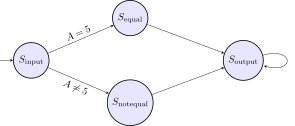
\includegraphics[width=257.9pt]{lect_9_if_then_else_fsm_no_extra}\caption{without wait state}\label{fig:ite-fsm-noextra}
\end{subfigure}
\\[6pt]
\begin{subfigure}[b]{271.2pt}\centering
  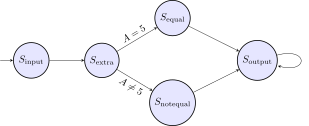
\includegraphics[width=269.2pt]{lect_9_if_then_else_fsm}\caption{with wait state}\label{fig:ite-fsm}
\end{subfigure}
\caption{Control-unit state diagrams for the if-then-else algorithm.}
\end{figure}

\begin{figure}[htbp]
\centering
\wavesplit{lect_9_if_then_else_no_wait}{2}\vspace{3pt}{\small (a)~without wait state: the wrong branch is taken}\\[6pt]
\wavesplit{lect_9_if_then_else_wait_state}{3}\vspace{3pt}{\small (b)~with wait state: the correct branch is taken}
\caption{Simulation waveforms of the if-then-else processor (author's screenshots).}
\label{fig:ite-nowait}\label{fig:ite-wait}
\end{figure}

\vhdlfile{listings/ch09_if_then_else_control.vhd}{Structural VHDL of the if-then-else control unit (state register of D flip-flops and the synthesised equations). The component \code{d_ff_r} is the flip-flop with asynchronous reset of \cref{lst:seqdet-struct}.}{lst:ite-cu}

\figw{410.0pt}{lect_9_if_then_else_combined}{The if-then-else control unit connected to its datapath.}{fig:ite-comb}

\subsection{Example 3: the GCD processor}
\begin{example}{Greatest common divisor}{gcd}
The \emph{greatest common divisor} of two positive integers $X$ and $Y$ can be found by repeated subtraction (Euclid's algorithm): the larger number is replaced by the difference until the two are equal.
\begin{center}\ttfamily\small
\begin{tabular}{@{}l@{}}
INPUT X\\ INPUT Y\\ WHILE (X != Y) \{\\ \quad IF (X > Y) THEN X = X - Y\\ \quad ELSE Y = Y - X\\ \}\\ OUTPUT X
\end{tabular}
\end{center}
For $X=25$, $Y=15$: $X>Y$, so $X=10$; $X<Y$, so $Y=5$; $X>Y$, so $X=5$; now $X=Y=5$, the GCD.

\textbf{Datapath} (\cref{fig:gcd-dp}): registers $X$ and $Y$, each with an input multiplexer that selects the external input or the result of the subtractor, a subtractor whose operands are chosen by multiplexers so that it can compute $X-Y$ or $Y-X$, and comparators that produce the status signals $XeqY$ and $XgtY$. The control signals are \textit{In\_X}, \textit{In\_Y} (select the external input, 1, or the subtractor result, 0), \textit{XLoad}, \textit{YLoad}, \textit{XY} (0: $X-Y$; 1: $Y-X$) and \textit{Out}.

\textbf{Control unit} (\cref{fig:gcd-fsm}). $S_0$ (init): load $X$ and $Y$ from the inputs. $S_1$ (check): compare; go to $S_4$ if $X=Y$, to $S_2$ if $X>Y$, otherwise to $S_3$. $S_2$: $X\leftarrow X-Y$, then back to $S_1$. $S_3$: $Y\leftarrow Y-X$, then back to $S_1$. $S_4$ (done): output the result. \Cref{lst:gcd-cu} is the VHDL of the control unit, with the control signals as Moore outputs. The datapath components and the top-level connection are in \cref{app:listings}, and \cref{fig:gcd-sim} shows the simulation.
\end{example}

\begin{figure}[htbp]
\centering
\begin{subfigure}[b]{412.0pt}\centering
  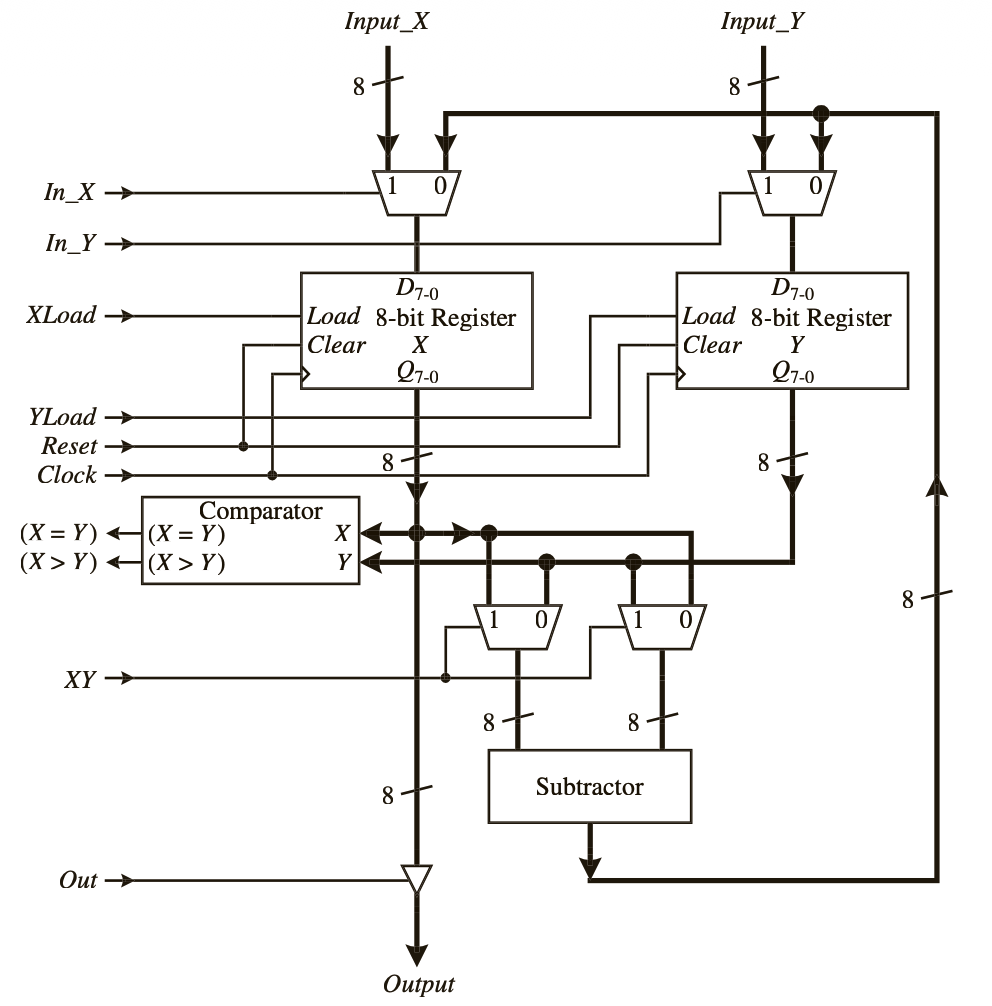
\includegraphics[width=399.0pt]{lect_9_gcd_datapath}\caption{datapath}\label{fig:gcd-dp}
\end{subfigure}
\caption{The GCD processor.}
\end{figure}

\begin{figure}[htbp]
\centering
\ContinuedFloat
\begin{subfigure}[b]{219.0pt}\centering
  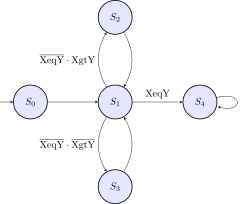
\includegraphics[width=217.0pt]{lect_9_gcd_fsm}\caption{control FSM}\label{fig:gcd-fsm}
\end{subfigure}
\caption[]{The GCD processor.}
\end{figure}

\vhdlfile{../vhdl/gcd/gcd_control.vhd}{VHDL of the GCD control unit (FSM with five states).}{lst:gcd-cu}

\begin{figure}[htbp]
\centering
\wavesplit{lect_9_gcd_sim}{5}
\caption{Simulation of the GCD processor (author's screenshot).}
\label{fig:gcd-sim}
\end{figure}

\section{FSM+D versus FSMD}\label{sec:fsmd}
There are two ways to describe a dedicated processor in an HDL.
\begin{description}[font=\sffamily\bfseries, leftmargin=1.2em]
  \item[FSM+D (FSM plus datapath)] The control unit (FSM) and the datapath are designed as \emph{separate, explicitly constructed} units and connected in a top-level module, as in the examples so far. The designer has full control over the datapath structure, which is useful for highly optimised or unusual datapaths.
  \item[FSMD (FSM with datapath)] The whole design is described as \emph{one behavioural FSM}, with the datapath operations (such as \code{X <= X - Y;}) written inside the states. The synthesis tool infers the registers, adders and multiplexers and connects them to the control logic. This is faster and simpler for standard operations and is the most common modern approach~\cite{gajski1997}.
\end{description}
\Cref{lst:gcd-fsmd} is the GCD calculator as an FSMD. The state diagram is the same as \cref{fig:gcd-fsm}, but each state now contains the register transfer it performs. Compare its length with the FSM+D version; the RTL viewer (\cref{fig:gcd-fsmd-rtl}) shows that the synthesis tool has generated the comparators, subtractors and registers by itself.

\vhdlfile{../vhdl/gcd_fsmd.vhd}{The GCD calculator as an FSMD: datapath operations inside a single behavioural state machine.}{lst:gcd-fsmd}

\begin{figure}[htbp]
\centering
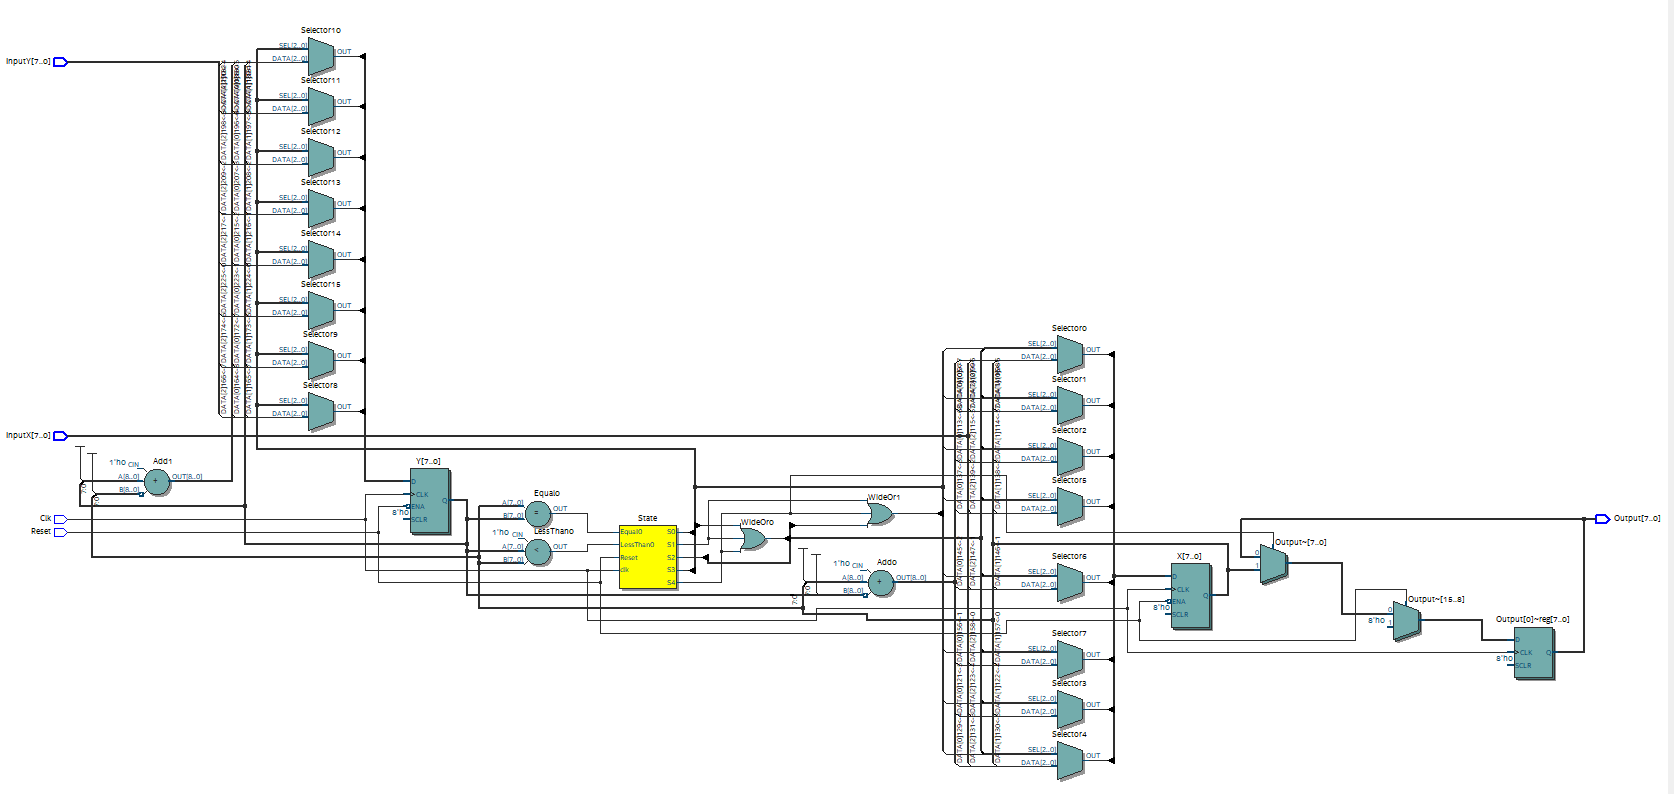
\includegraphics[width=0.9\linewidth]{lect_9_gcd_fsmd}\\[6pt]
\foreach \wsi in {1,...,4}{\includegraphics[width=\linewidth,height=95pt,keepaspectratio]{lect_9_gcd_fsmd_sim_p\wsi}\par\vspace{1.5pt}}
\caption{The FSMD GCD: logic diagram from the Quartus RTL viewer (top) and simulation (bottom). Author's screenshots.}
\label{fig:gcd-fsmd-rtl}
\end{figure}

\begin{chaptersummary}
\begin{itemize}
  \item The \textbf{von Neumann model} has input, output, memory and a microprocessor made of a \textbf{datapath} and a \textbf{control unit}. A \textbf{dedicated microprocessor} hardwires a single algorithm.
  \item The \textbf{datapath} (registers, adders, multiplexers, comparators) performs the data operations; the \textbf{control unit} is an FSM that sends \textbf{control signals} and receives \textbf{status signals}.
  \item At the \textbf{RTL}, a computation is a sequence of register transfers $R_1\leftarrow f(R_2,R_3)$.
  \item Each instruction of an algorithm becomes a \textbf{control word}; multiplexers let one functional unit serve several operations.
  \item The control unit's FSM has one state per control word; the next-state logic uses status signals. A \textbf{wait state} is required when a decision depends on a register loaded in the preceding state.
  \item \textbf{FSM+D} builds the datapath and control unit explicitly; \textbf{FSMD} describes everything as one behavioural FSM and lets the tool infer the datapath.
\end{itemize}
\end{chaptersummary}

\chapsec{Exercises}
\begin{exlist}
  \item \textbf{Datapath design.} Draw a dedicated datapath that performs $R_1\leftarrow R_1-R_2$. List the control signals.
  \item \textbf{Control signals.} In the shared-adder datapath of \cref{fig:dp-shared}, suppose the two multiplexers had separate select signals $Mux1$ (first multiplexer: $0=B$, $1=A$) and $Mux2$ (second multiplexer: $0=C$, $1$ = constant 3). Give the values of $Mux1$, $Mux2$ and $ALoad$ that perform $A=B+3$.
  \item \textbf{Conditional logic.} What hardware must be added to a datapath to support the instruction \textbf{IF} $(A>10)$ \textbf{THEN}~\dots? Which signal is delivered to the control unit?
  \item \textbf{Control-word sequence.} Write the control-word sequence for \emph{swapping} the contents of registers $A$ and $B$, assuming a temporary register $Temp$. Define the control signals and give one control word per step.
  \item Write the control words and draw the FSM of the control unit for the summation algorithm of \cref{tab:cw-sum}. How many states are needed? What is the status signal and in which state is it examined?
  \item Trace Euclid's algorithm for $(X,Y)=(12,18)$ and $(X,Y)=(48,18)$. Count the number of clock cycles the FSM of \cref{fig:gcd-fsm} takes (from $S_0$ to the first cycle in $S_4$).
  \item Draw a datapath for $F\leftarrow(A+B)-C$ with one adder/subtractor and one result register. Write the sequence of control words.
  \item Derive the next-state equations $D_2,D_1,D_0$ of the if-then-else control unit from \cref{tab:ite-ns}. Verify that the unused states 101, 110 and 111 do or do not lead to a valid state, and discuss.
  \item Explain in your own words why the if-then-else control unit needs the state $S_{extra}$, with a timing sketch of the register load and the comparator output.
  \item Rewrite the if-then-else processor as an FSMD in VHDL: a single process with the states \textit{input}, \textit{extra}, \textit{equal}, \textit{notequal}, \textit{output}.
  \item Write an FSMD in VHDL that computes $Sum=1+2+\dots+10$ and presents the result in the last state.
  \item Compare FSM+D and FSMD for a GCD processor: which would you use to build a processor whose adders must be hand-placed on an FPGA to meet timing, and why?
\end{exlist}

\chapsec{Further Reading}
The method of designing a processor as a datapath and a control unit, with control words and status signals, follows Hwang~\cite{hwang2018,hwang2005}. The FSMD model is described by Gajski~\cite{gajski1997} and by Harris and Harris~\cite{harris2012}, who give a good account of the relation between architecture and microarchitecture; Brown and Vranesic~\cite{brown2009} discuss datapath/controller design in their treatment of simple processors.

\chapter{General-Purpose Microprocessors}\label{ch:gp}

\begin{objectives}
After studying this chapter you will be able to:
\begin{itemize}
  \item explain how a general-purpose processor differs from a dedicated one, and describe the instruction cycle (fetch, decode, execute);
  \item define an instruction set and its binary encoding;
  \item describe the datapath and control unit of the simple processors EC-1 and EC-2 and trace the execution of a program;
  \item explain why the control unit needs wait states when memory is synchronous;
  \item write, assemble and trace small programs in machine code, and load them into memory with an Intel HEX file; and
  \item describe how the step from ROM to RAM leads to the von Neumann stored-program computer.
\end{itemize}
\end{objectives}

\section{General-Purpose Microprocessors}
The dedicated processors of \cref{ch:dedicated} perform one task, wired into their structure. A \term{general-purpose microprocessor} can perform many different functions: its function is determined by the \emph{instructions} it executes, which are stored in memory as a \term{program}. Changing the program changes the function without changing the hardware. The Intel Core and ARM Cortex processors are examples.

\begin{keypoint}[A processor is a dedicated processor]
A general-purpose processor can be viewed as a \emph{dedicated} processor whose single task is to \textbf{fetch and execute instructions}. The ``data'' that it processes include the instructions themselves.
\end{keypoint}

We therefore design it with the methods of the previous chapter. The designs of this chapter, the 8-bit processors \textbf{EC-1} and \textbf{EC-2}, follow the educational processor designs of Hwang~\cite{hwang2005,hwang2018}; the structure, the VHDL descriptions, the programs and the simulations presented here are the author's implementations for this course.

\section{Overview of CPU Design}\label{sec:cpu-design}
Designing a central processing unit (CPU) has three steps.
\begin{enumerate}
  \item \textbf{Define the instruction set}: the operations the processor performs (add, load, jump, \dots) and how each instruction is encoded in binary (an \term{opcode} and its \term{operands}).
  \item \textbf{Design the datapath}: a datapath that can execute \emph{every} instruction of the set. It contains the \term{program counter} (PC), which holds the address of the next instruction; the \term{instruction register} (IR), which holds the current instruction; the ALU or other functional units; registers; and memory.
  \item \textbf{Design the control unit}: an FSM that executes the \term{instruction cycle}: \textbf{fetch} the instruction from memory (at the address in the PC) into the IR, \textbf{decode} it by examining the opcode, and \textbf{execute} it by issuing the control signals for the operation.
\end{enumerate}

\section{The EC-1 Microprocessor}\label{sec:ec1}
\subsection{Overview}
To keep the design small enough to do by hand, EC-1 is a simple 8-bit processor with:
\begin{itemize}
  \item an \textbf{8-bit} data width;
  \item a \textbf{4-bit} address, hence $2^4=16$ memory words;
  \item a \textbf{read-only memory} (ROM) that holds the program; and
  \item one data register, the \term{accumulator} $A$.
\end{itemize}
It is an \emph{accumulator machine}: every operation takes its operand from, and returns its result to, register $A$.

\subsection{Instruction set}
EC-1 has only five instructions. The opcode occupies the 3 most significant bits of the 8-bit instruction (\cref{tab:ec1-is}). Opcodes 000, 001 and 010 are unused (no operation); the bits shown as \texttt{x} are don't-cares and \texttt{aaaa} is a 4-bit address.

\begin{table}[htbp]
\centering
\caption{The EC-1 instruction set.}
\label{tab:ec1-is}
\begin{tabular}{llll}
\toprule
Mnemonic & Encoding & Operation & Description\\ \midrule
\texttt{IN A} & \texttt{011 xxxxx} & $A\leftarrow$ Input & input a byte into $A$\\
\texttt{OUT A} & \texttt{100 xxxxx} & Output $\leftarrow A$ & output $A$\\
\texttt{DEC A} & \texttt{101 xxxxx} & $A\leftarrow A-1$ & decrement $A$\\
\texttt{JNZ addr} & \texttt{110 xaaaa} & if $A\neq0$, $PC\leftarrow aaaa$ & jump if not zero\\
\texttt{HALT} & \texttt{111 xxxxx} & halt & stop execution\\ \bottomrule
\end{tabular}
\end{table}

\subsection{Datapath}
The datapath (\cref{fig:ec1-dp}) must support fetching instructions and executing them.
\begin{itemize}
  \item The \textbf{program counter} PC (4 bits) addresses the ROM. Normally $PC\leftarrow PC+1$ (the incrementer). For \texttt{JNZ} with $A\neq0$, $PC\leftarrow IR[3:0]$; the multiplexer \textit{JNZmux} chooses between the incremented PC and the jump address.
  \item The \textbf{instruction register} IR (8 bits) holds the instruction read from the ROM. Its top three bits $IR[7:5]$ are the opcode that goes to the control unit.
  \item The \textbf{accumulator} $A$ (8 bits) takes its input either from the external input port or from the decrementer ($A-1$); the multiplexer \textit{INmux} chooses ($1$ = Input, $0$ = Dec).
  \item A \textbf{zero detector} (an 8-input OR gate on $A$) generates the status signal $A\neq0$ for the control unit.
  \item A \textbf{three-state buffer} controlled by \textit{OutE} drives the output port with $A$.
\end{itemize}
The control signals, produced by the control unit, are \textit{IRload}, \textit{PCload}, \textit{INmux}, \textit{Aload}, \textit{JNZmux}, \textit{OutE} and \textit{Halt}.

\begin{sidewaysfigure}[p]
\centering
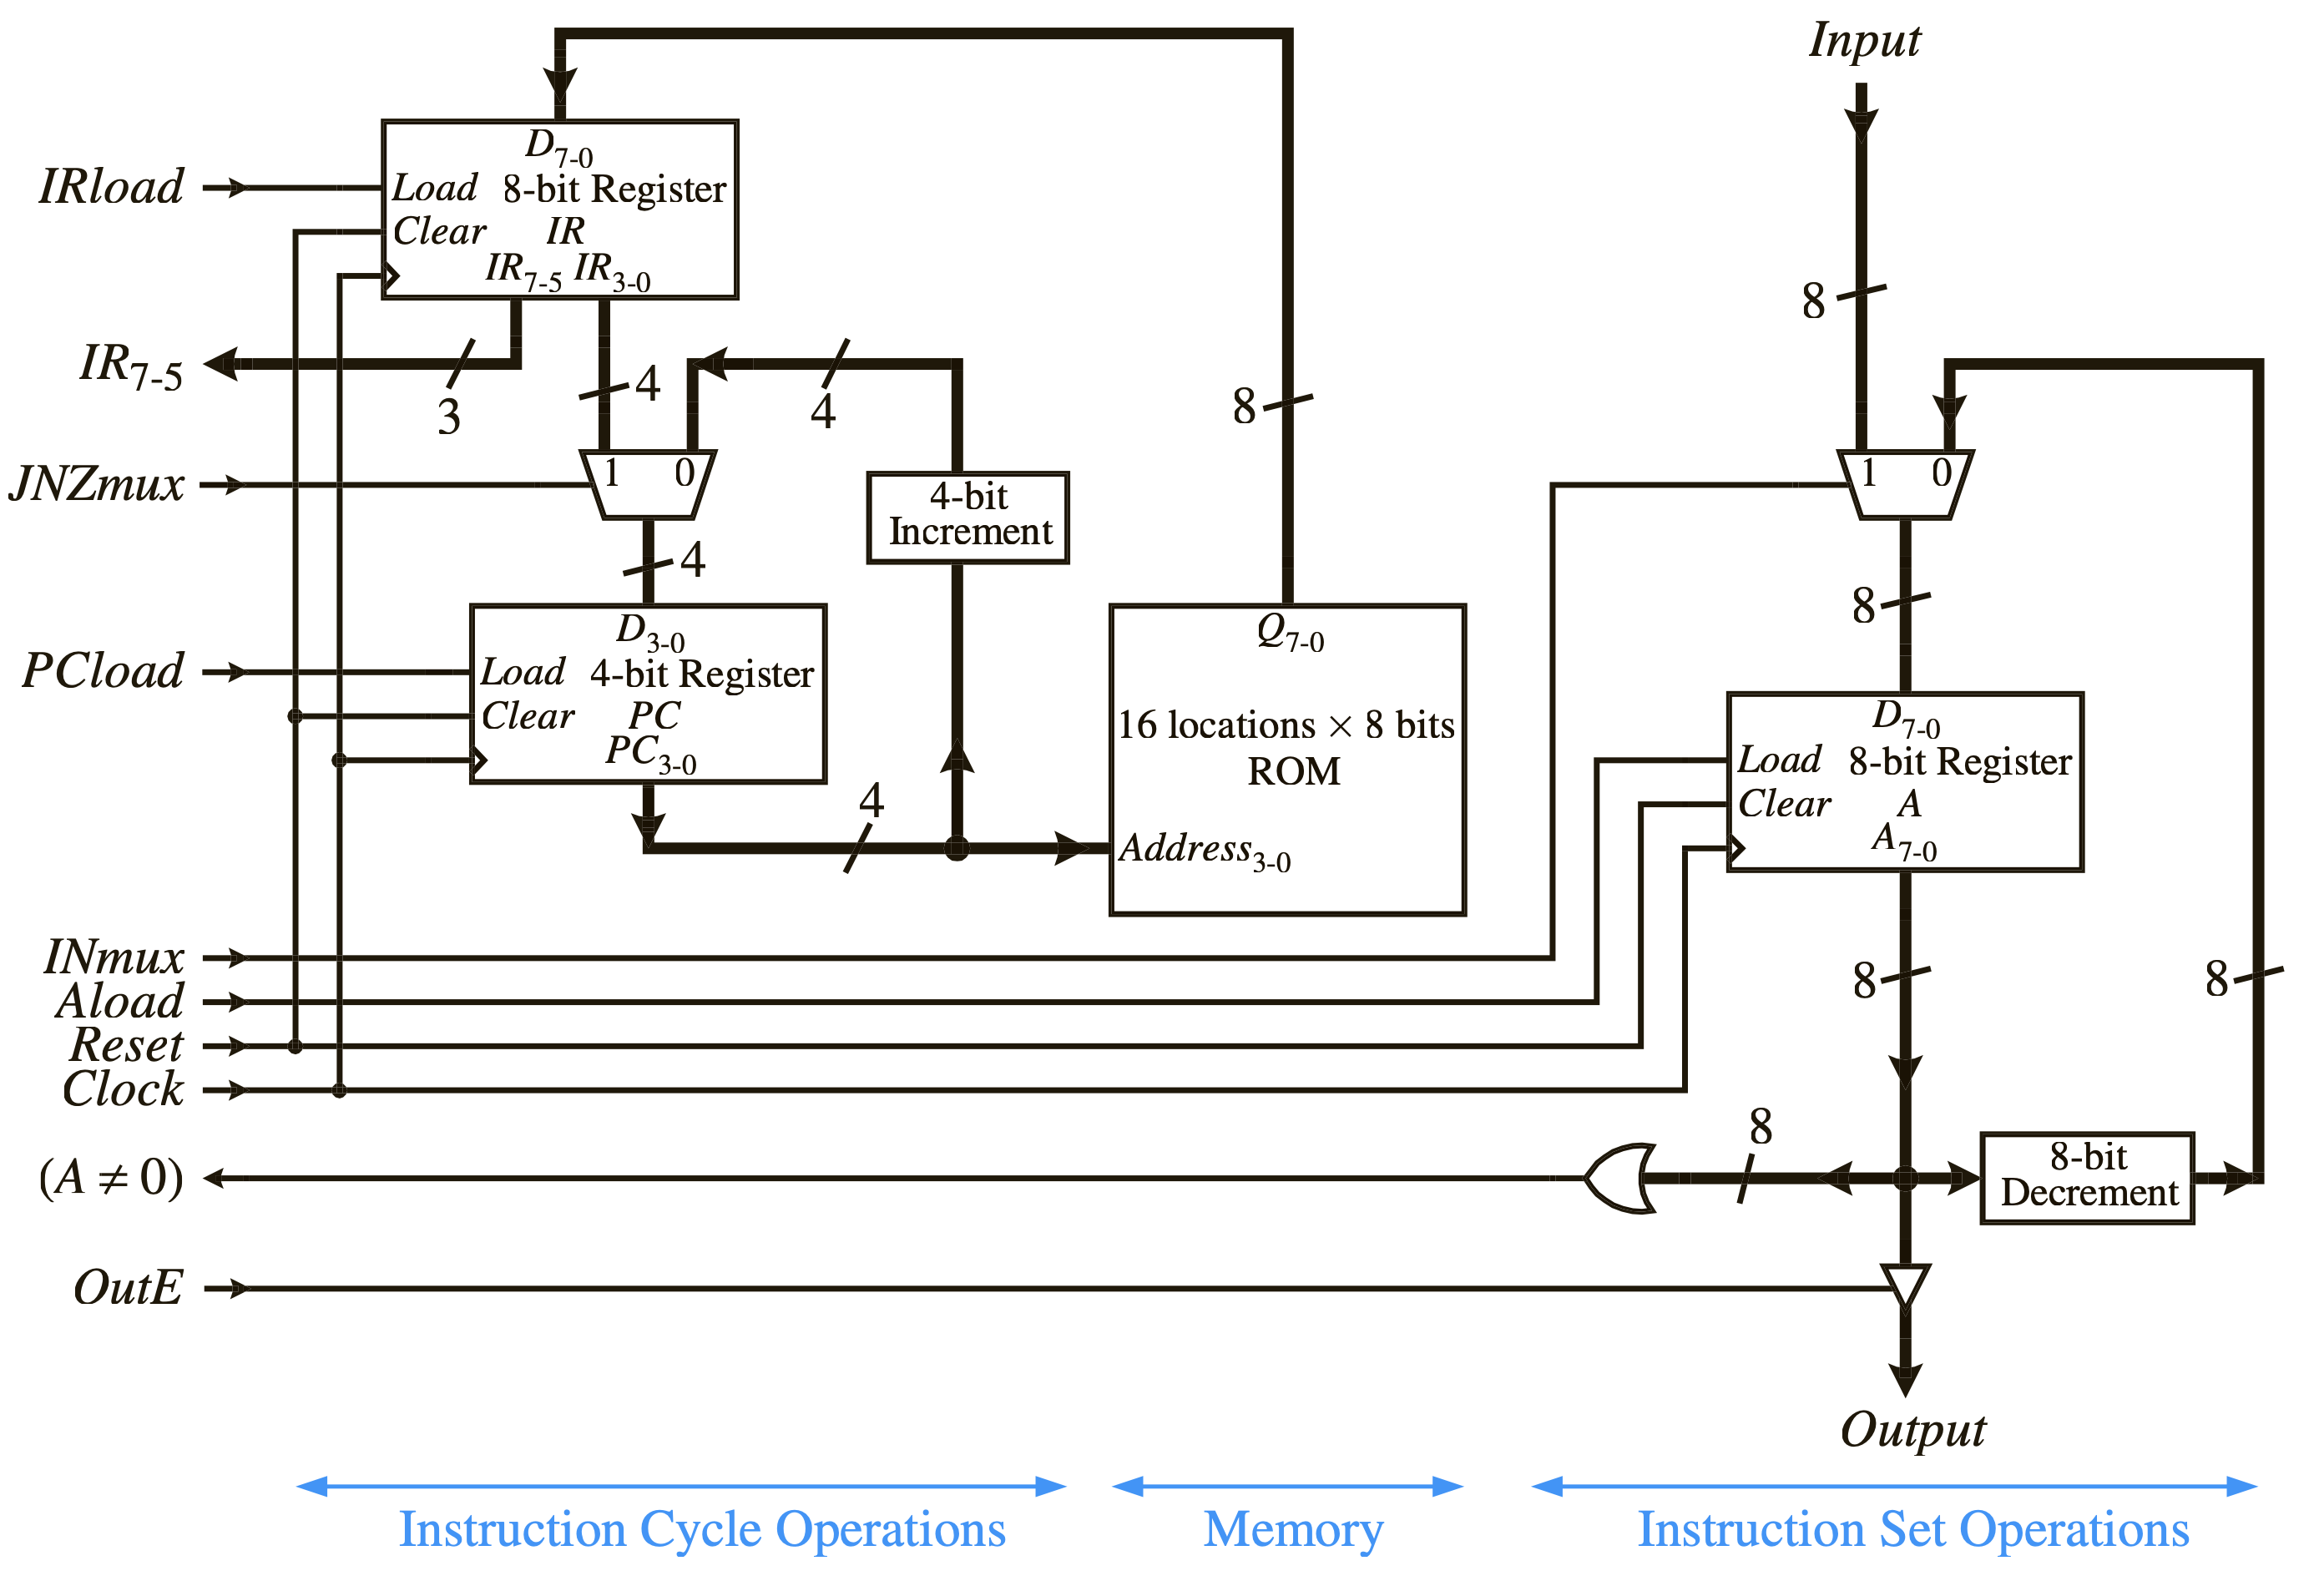
\includegraphics[width=\linewidth, height=415pt, keepaspectratio]{lect_10_ec1_datapath}
\caption{Datapath of the EC-1 microprocessor. Multiplexer inputs are numbered $1$ (left) and $0$ (right); a slash on a bus gives its width in bits. The clock and the reset are common to all registers, and the control signals (left) come from the control unit.}
\label{fig:ec1-dp}
\end{sidewaysfigure}

\subsection{ROM implementation}
FPGA vendors provide optimised memory blocks as \emph{IP cores} (intellectual-property modules). Using them guarantees that the memory is mapped to the FPGA's dedicated block-RAM resources rather than to general logic cells. In our implementation the program ROM is a one-port ROM generated by Intel's megafunction wizard (type \code{altsyncram}): an 8-bit wide, 32-word memory with a single clock and \emph{unregistered} output, initialised at programming time from a file in Intel HEX format. The memory is \emph{synchronous}: the address is sampled on the rising clock edge. As we shall see, this has consequences for the control unit.

\subsection{Intel HEX format}
\term{Intel HEX} is a text format that stores binary data for programming or initialising memories. Each line is a \emph{record} beginning with a colon: \texttt{:}\,\textit{LL}\,\textit{AAAA}\,\textit{TT}\,\textit{DD\dots DD}\,\textit{CC}, where \textit{LL} is the number of data bytes, \textit{AAAA} the starting address, \textit{TT} the record type (00 = data, 01 = end of file), \textit{DD} the data bytes and \textit{CC} a checksum chosen so that the sum of all bytes of the record is $00_{16}$ modulo 256. For example, the line
\begin{center}\ttfamily\small :100000006080A0C1E00000000000000000000000CF\end{center}
holds 16 (\texttt{10}$_{16}$) bytes starting at address 0000, the first five being the program of \cref{tab:ec1-prog}; its checksum is $\mathrm{CF}$ because $10+00+00+00+60+80+A0+C1+E0=331_{16}$ and $100_{16}-31_{16}=\mathrm{CF}_{16}$. The file is completed by a record for addresses 16--31 and the end-of-file record \texttt{:00000001FF}.

\subsection{Control unit}
The control unit is an FSM that carries out the instruction cycle, with one \textbf{fetch} state, one \textbf{decode} state and one execution state for each instruction (\cref{fig:ec1-fsm-nowait}).
\begin{description}[font=\sffamily\bfseries, leftmargin=1.2em]
  \item[FETCH (000)] Read the instruction at address PC into IR ($IR\leftarrow M[PC]$) and increment the PC ($PC\leftarrow PC+1$): $IRload=PCload=1$, $JNZmux=0$.
  \item[DECODE (001)] Examine the opcode $IR[7:5]$ and go to the execution state of the instruction (no control signals). Unused opcodes return to FETCH.
  \item[EXECUTE] \textbf{Input} (011): $A\leftarrow$ Input, $INmux=1$, $Aload=1$. \textbf{Output} (100): $OutE=1$. \textbf{Dec} (101): $A\leftarrow A-1$, $INmux=0$, $Aload=1$. \textbf{JNZ} (110): if $A\neq0$ then $PC\leftarrow IR[3:0]$ ($JNZmux=1$, $PCload=1$). \textbf{Halt} (111): stay here.
\end{description}
All execution states except Halt return to FETCH. The values of the control signals in each state are in \cref{tab:ec1-cs}.

\begin{table}[htbp]
\centering
\small
\caption{Control signals of the EC-1 in each state (``--'' = don't care).}
\label{tab:ec1-cs}
\begin{tabular}{lc|ccccccc}
\toprule
State & Code & IRload & PCload & INmux & Aload & JNZmux & OutE & Halt\\ \midrule
Fetch & 000 & 1 & 1 & -- & 0 & 0 & 0 & 0\\
Decode & 001 & 0 & 0 & -- & 0 & 0 & 0 & 0\\
Wait & 010 & 0 & 0 & -- & 0 & 0 & 0 & 0\\
Input & 011 & 0 & 0 & 1 & 1 & 0 & 0 & 0\\
Output & 100 & 0 & 0 & -- & 0 & 0 & 1 & 0\\
Decrement & 101 & 0 & 0 & 0 & 1 & 0 & 0 & 0\\
JumpNotZero & 110 & 0 & $(A\neq0)$ & -- & 0 & 1 & 0 & 0\\
Halt & 111 & 0 & 0 & -- & 0 & 0 & 0 & 1\\ \bottomrule
\end{tabular}
\end{table}

\subsubsection{The wait state}
The EC-1 uses a \emph{synchronous} ROM: it samples the address at the clock edge. In normal execution the PC is stable throughout the execution state, so the next fetch reads the right instruction. But when a jump is \emph{taken}, the PC is updated with the target address at the clock edge at the \emph{end} of the JNZ state. If the next state were FETCH, the ROM would sample the PC at the \emph{same edge} at which the PC changes, and may read the old address: a race condition. The solution is a \textbf{wait state}: JNZ goes to WAIT (010), a buffer cycle in which all control signals are idle, while the PC settles at the target; WAIT then goes to FETCH, in which the ROM safely samples the stable address (\cref{fig:ec1-fsm}). This is the same idea as the wait state of \cref{ex:cu2}.

\begin{figure}[htbp]
\centering
\begin{subfigure}[b]{396.7pt}\centering
  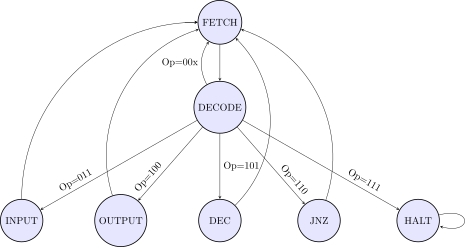
\includegraphics[width=394.7pt]{lect_10_ec1_fsm_no_wait}\caption{without wait state}\label{fig:ec1-fsm-nowait}
\end{subfigure}
\caption{State diagram of the EC-1 control unit.}
\end{figure}

\begin{figure}[htbp]
\centering
\ContinuedFloat
\begin{subfigure}[b]{396.7pt}\centering
  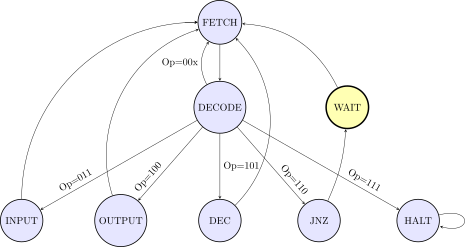
\includegraphics[width=394.7pt]{lect_10_ec1_fsm}\caption{with wait state}\label{fig:ec1-fsm}
\end{subfigure}
\caption[]{State diagram of the EC-1 control unit.}
\end{figure}

\subsubsection{State table and equations}
With the state codes of \cref{tab:ec1-cs}, and $O_2O_1O_0$ the opcode, the next-state equations follow from the state diagram:
\begin{align*}
 D_2 &= \mathrm{Decode}\cdot O_2 + \mathrm{Halt},\\
 D_1 &= \mathrm{Decode}\cdot O_1\cdot(O_2+O_0) + \mathrm{Halt} + \mathrm{JNZ},\\
 D_0 &= \mathrm{Fetch} + \mathrm{Decode}\cdot O_0\cdot(O_2+O_1) + \mathrm{Halt},
\end{align*}
where the state decoders are $\mathrm{Fetch}=Q_2'Q_1'Q_0'$, $\mathrm{Decode}=Q_2'Q_1'Q_0$, $\mathrm{Input}=Q_2'Q_1Q_0$, $\mathrm{Output}=Q_2Q_1'Q_0'$, $\mathrm{Dec}=Q_2Q_1'Q_0$, $\mathrm{JNZ}=Q_2Q_1Q_0'$ and $\mathrm{Halt}=Q_2Q_1Q_0$. Each term can be checked against \cref{fig:ec1-fsm}: for instance $D_1=1$ in the JNZ state because the next state is WAIT ($010$); in the decode state $D_1=1$ for the opcodes 011 (Input $=011$), 110 (JNZ $=110$) and 111 (Halt $=111$) but not 010 (unused, back to Fetch). WAIT and the other states return to $000$ by $D_2=D_1=D_0=0$. The outputs are
\begin{gather*}
 IRload = \mathrm{Fetch},\quad PCload = \mathrm{Fetch} + \mathrm{JNZ}\cdot(A\neq0),\quad INmux = \mathrm{Input},\\
 Aload = \mathrm{Input}+\mathrm{Dec},\quad JNZmux=\mathrm{JNZ},\quad OutE=\mathrm{Output},\quad Halt=\mathrm{Halt}.
\end{gather*}
\Cref{lst:ec1-cu} is the VHDL of the control unit; it is written directly from these equations (structural style), using three D flip-flops. \Cref{lst:ec1-dp} is the datapath. The components (flip-flops, registers, multiplexers, incrementer, decrementer, zero detector, three-state buffer) and the top level, which connects the two, are listed in \cref{app:listings}.

\vhdlfile{../vhdl/ec1_control_unit.vhd}{VHDL of the EC-1 control unit (structural, from the state equations).}{lst:ec1-cu}
\vhdlfile{../vhdl/ec1_datapath.vhd}{VHDL of the EC-1 datapath.}{lst:ec1-dp}

\subsection{Programming example: countdown from 10 to 1}
A program for EC-1 is a list of instruction bytes. \Cref{tab:ec1-prog} counts down from the input value to 1, outputting each value: \texttt{IN A} reads the starting value, \texttt{OUT A} displays $A$, \texttt{DEC A} decrements it, \texttt{JNZ 01} returns to \texttt{OUT A} while $A\neq0$, and \texttt{HALT} stops. Instructions are encoded by \cref{tab:ec1-is}; for example \texttt{JNZ 01} $=\texttt{110\,0\,0001}=\mathrm{C1}$.

\begin{table}[htbp]
\centering
\caption{EC-1 program: count down from the input value.}
\label{tab:ec1-prog}
\begin{tabular}{ccll}
\toprule Address & Hex & Assembly & Comment\\ \midrule
00 & 60 & \texttt{IN A} & input to $A$\\
01 & 80 & \texttt{OUT A} & output $A$\\
02 & A0 & \texttt{DEC A} & decrement $A$\\
03 & C1 & \texttt{JNZ 01} & jump to 01 if $A\ne0$\\
04 & E0 & \texttt{HALT} & done\\ \bottomrule
\end{tabular}
\end{table}

A testbench (similar to \cref{lst:tb}) generates a clock of period 10~ns, holds the reset for 20~ns, applies the input value 10 ($\bin{00001010}$) and runs until the \textit{halt} output is 1. \Cref{fig:ec1-sim} shows the result: the output counts $10,9,\dots,2,1$. For every value the processor goes through FETCH, DECODE and the execution state of \texttt{OUT A}, FETCH, DECODE, \texttt{DEC A}, FETCH, DECODE, \texttt{JNZ} and, when the jump is taken, WAIT; when $A$ reaches 0 the jump is not taken, PC advances to 04 and \texttt{HALT} is executed. The RTL viewer of Quartus shows the synthesised top level (\cref{fig:ec1-rtl}).

\begin{figure}[htbp]
\centering
{\small (a)~start: counting 10, 9, \dots}\\[3pt]
\wavestrip{lect_10_ec-1_count_10_9}{1}{175}
\wavestrip{lect_10_ec-1_count_10_9}{2}{175}
\wavestrip{lect_10_ec-1_count_10_9}{3}{175}
\caption{Simulation of the EC-1 running the countdown program (author's screenshots).}
\label{fig:ec1-sim}
\end{figure}

\begin{figure}[htbp]
\centering
\ContinuedFloat
\wavestrip{lect_10_ec-1_count_10_9}{4}{175}
\wavestrip{lect_10_ec-1_count_10_9}{5}{175}
\vspace{4pt}{\small (b)~end: \dots, 2, 1 and halt}\\[3pt]
\wavestrip{lect_10_ec-1_count_2_1}{1}{167}
\caption[]{Simulation of the EC-1 running the countdown program (author's screenshots).}
\end{figure}

\begin{figure}[htbp]
\centering
\ContinuedFloat
\wavestrip{lect_10_ec-1_count_2_1}{2}{167}
\wavestrip{lect_10_ec-1_count_2_1}{3}{167}
\wavestrip{lect_10_ec-1_count_2_1}{4}{167}
\caption[]{Simulation of the EC-1 running the countdown program (author's screenshots).}
\end{figure}

\begin{figure}[htbp]
\centering
\ContinuedFloat
\wavestrip{lect_10_ec-1_count_2_1}{5}{167}
\caption[]{Simulation of the EC-1 running the countdown program (author's screenshots).}
\end{figure}

\figw{\linewidth}{lect_10_rtl_viewer_ec-1}{RTL viewer (Quartus) of the top level of the EC-1: the control unit and the datapath (author's screenshot).}{fig:ec1-rtl}

\section{The EC-2 Microprocessor}\label{sec:ec2}
\subsection{Overview}
EC-2 improves on EC-1 in two ways: more instructions and a \emph{read/write} memory that stores both code and data. This is a \emph{stored-program computer} in the von Neumann sense (\cref{fig:vn-ec2}). EC-2 has
\begin{itemize}
  \item eight instructions;
  \item a $32\times8$-bit \textbf{RAM} that holds both the program and its variables (unified code/data memory);
  \item a \textbf{5-bit} address; and
  \item an adder/subtractor ALU.
\end{itemize}

\figw{191.1pt}{lect_10_von_neumann}{The von Neumann architecture: a single memory holds instructions and data, connected to the processor by a common bus.}{fig:vn-ec2}

\subsection{Instruction set}
\Cref{tab:ec2-is} lists the instructions. The three most significant bits are the opcode and the five least significant bits the memory address \texttt{aaaaa}. Memory operands make this a \emph{memory-reference} machine. \texttt{JZ} jumps if $A=0$ and \texttt{JPOS} if $A\ge0$ (a non-negative two's-complement value).

\begin{table}[htbp]
\centering
\caption{The EC-2 instruction set.}
\label{tab:ec2-is}
\begin{tabular}{llll}
\toprule
Mnemonic & Encoding & Operation & Description\\ \midrule
\texttt{LOAD A, addr} & \texttt{000 aaaaa} & $A\leftarrow M[aaaaa]$ & load $A$ from memory\\
\texttt{STORE A, addr} & \texttt{001 aaaaa} & $M[aaaaa]\leftarrow A$ & store $A$ to memory\\
\texttt{ADD A, addr} & \texttt{010 aaaaa} & $A\leftarrow A+M[aaaaa]$ & add memory to $A$\\
\texttt{SUB A, addr} & \texttt{011 aaaaa} & $A\leftarrow A-M[aaaaa]$ & subtract memory from $A$\\
\texttt{IN A} & \texttt{100 xxxxx} & $A\leftarrow$ Input & input to $A$\\
\texttt{JZ addr} & \texttt{101 aaaaa} & if $A=0$, $PC\leftarrow aaaaa$ & jump if zero\\
\texttt{JPOS addr} & \texttt{110 aaaaa} & if $A\ge0$, $PC\leftarrow aaaaa$ & jump if non-negative\\
\texttt{HALT} & \texttt{111 xxxxx} & halt & stop execution\\ \bottomrule
\end{tabular}
\end{table}

\subsection{Datapath}
The datapath (\cref{fig:ec2-dp}) is that of EC-1 with the following changes.
\begin{enumerate}
  \item A \textbf{5-bit address bus} to address 32 locations; the PC and IR address fields are 5 bits wide.
  \item A \textbf{RAM} instead of the ROM, so that \texttt{STORE} is possible.
  \item A \textbf{memory-address multiplexer} (\textit{MemInst}): during \emph{fetch} the address comes from the PC ($0$); during the execution of LOAD, STORE, ADD and SUB it comes from $IR[4:0]$ ($1$). This shared address bus is the fundamental constraint of the von Neumann design.
  \item An \textbf{ALU} that adds ($\mathit{Sub}=0$) or subtracts ($\mathit{Sub}=1$) the RAM output from $A$.
  \item A \textbf{4-to-1 accumulator multiplexer} (\textit{Asel}) that selects the input of $A$: the RAM output (LOAD, $00$), the ALU output (ADD, SUB, $01$) or the input port (IN, $10$); code $11$ selects the constant 0.
  \item Flag detectors for $A=0$ (\textit{Zero}, an 8-input NOR gate) and $A\ge0$ (\textit{Pos}, the inverted sign bit $A_7$), the status signals for JZ and JPOS.
\end{enumerate}
The control signals are \textit{IRload}, \textit{PCload}, \textit{MemInst}, \textit{MemWr} (RAM write enable), \textit{Asel}, \textit{Aload}, \textit{Sub}, \textit{JMPmux} (selects the jump address as the new PC) and \textit{Halt}.

\begin{sidewaysfigure}[p]
\centering
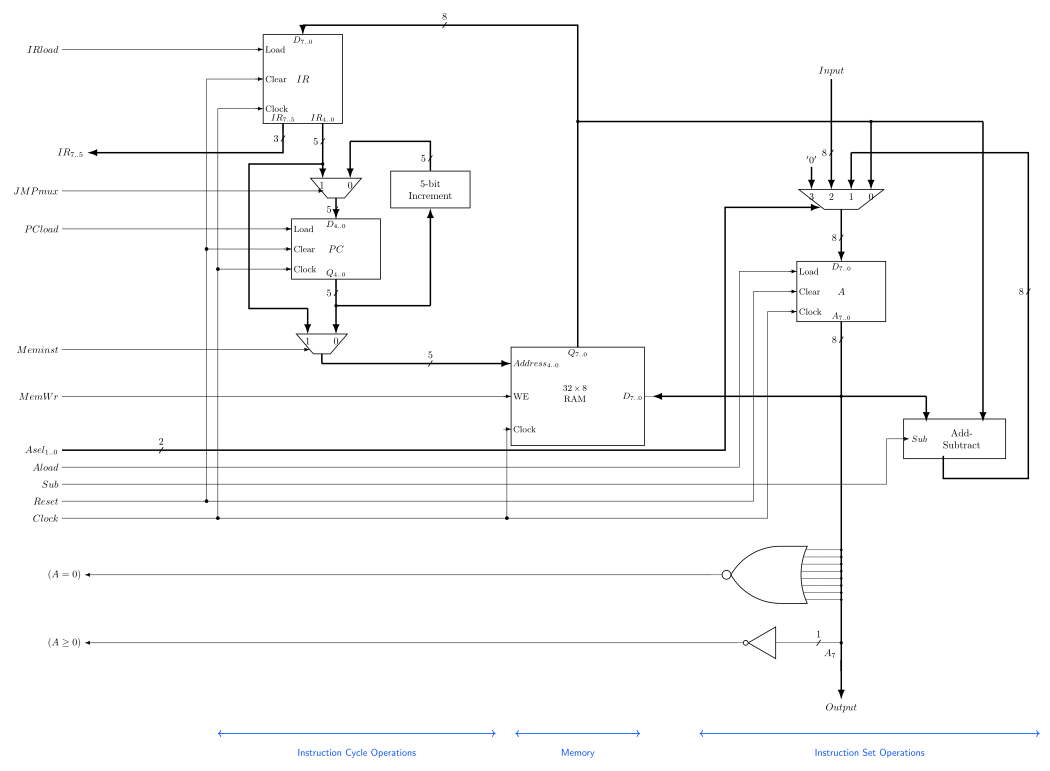
\includegraphics[width=\linewidth, height=425pt, keepaspectratio]{lect_10_ec2_datapath}
\caption{Datapath of the EC-2 microprocessor. The memory-address multiplexer \textit{MemInst} selects the PC (0) in the fetch state and the address field of the IR (1) when a memory operand is accessed; the accumulator multiplexer is selected by $Asel_{1..0}$ ($00$ RAM, $01$ ALU, $10$ input port, $11$ constant $0$). $(A=0)$ and $(A\ge0)$ are the status signals for \texttt{JZ} and \texttt{JPOS}.}
\label{fig:ec2-dp}
\end{sidewaysfigure}

\subsection{Control unit}
The instruction cycle now includes memory access (\cref{tab:ec2-cs}). In \textbf{fetch} ($\mathit{MemInst}=0$) the instruction is read from the address in the PC into IR and the PC is incremented. In \textbf{decode} the opcode selects the execution state. In \textbf{execute}: \texttt{LOAD} sets $MemInst=1$, reads the RAM and loads $A$; \texttt{STORE} sets $MemInst=1$ and $MemWr=1$, writing $A$ into the RAM; \texttt{ADD} and \texttt{SUB} set $MemInst=1$, read the RAM and load $A$ with the ALU result; \texttt{IN} loads $A$ from the input port; \texttt{JZ} and \texttt{JPOS} load the PC with the address field if the flag $Z$ or $P$ is true; \texttt{HALT} stops. The FSM is \cref{fig:ec2-fsm}, with ten states coded in 4 bits.

\begin{table}[htbp]
\centering
\scriptsize
\caption{Control signals of the EC-2 in each state ($Z$: $A=0$; $P$: $A\ge0$).}
\label{tab:ec2-cs}
\setlength{\tabcolsep}{3.5pt}
\begin{tabular}{lc|cccccccccc}
\toprule
State & Code & IRload & PCload & MemInst & MemWr & Asel & Aload & Sub & JMPmux & Halt\\ \midrule
Fetch & 0000 & 1 & 1 & 0 & 0 & -- & 0 & 0 & 0 & 0\\
Decode & 0001 & 0 & 0 & 0 & 0 & -- & 0 & 0 & 0 & 0\\
Load & 0010 & 0 & 0 & 1 & 0 & 00 & 1 & 0 & 0 & 0\\
Store & 0011 & 0 & 0 & 1 & 1 & -- & 0 & 0 & 0 & 0\\
Add & 0100 & 0 & 0 & 1 & 0 & 01 & 1 & 0 & 0 & 0\\
Sub & 0101 & 0 & 0 & 1 & 0 & 01 & 1 & 1 & 0 & 0\\
In & 0110 & 0 & 0 & 0 & 0 & 10 & 1 & 0 & 0 & 0\\
Jz & 0111 & 0 & $Z$ & 0 & 0 & -- & 0 & 0 & 1 & 0\\
Jpos & 1000 & 0 & $P$ & 0 & 0 & -- & 0 & 0 & 1 & 0\\
Halt & 1001 & 0 & 0 & 0 & 0 & -- & 0 & 0 & 0 & 1\\ \bottomrule
\end{tabular}
\end{table}

\begin{figure}[htbp]
\centering
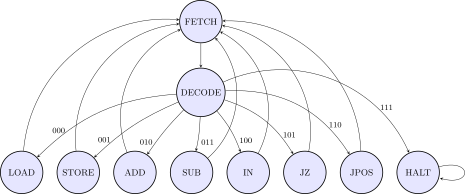
\includegraphics[max width=0.9\linewidth, max height=9cm]{lect_10_ec2_fsm}
\caption{State diagram of the EC-2 control unit.}
\label{fig:ec2-fsm}
\end{figure}

With the state codes of \cref{tab:ec2-cs}, and the opcode $O_2O_1O_0$ examined in the decode state, the next-state equations are
\begin{align*}
 D_3 &= \mathrm{Decode}\cdot O_2O_1 + \mathrm{Halt}, & D_2 &= \mathrm{Decode}\cdot(O_2\xor O_1),\\
 D_1 &= \mathrm{Decode}\cdot O_1', & D_0 &= \mathrm{Fetch} + \mathrm{Decode}\cdot O_0 + \mathrm{Halt},
\end{align*}
and the outputs are
\begin{gather*}
 IRload=\mathrm{Fetch},\quad PCload=\mathrm{Fetch}+\mathrm{Jz}\cdot Z+\mathrm{Jpos}\cdot P,\quad JMPmux=\mathrm{Jz}+\mathrm{Jpos},\\
 MemInst=\mathrm{Load}+\mathrm{Store}+\mathrm{Add}+\mathrm{Sub},\quad MemWr=\mathrm{Store},\\
 Asel_1=\mathrm{In},\quad Asel_0=\mathrm{Add}+\mathrm{Sub},\quad Aload=\mathrm{Load}+\mathrm{Add}+\mathrm{Sub}+\mathrm{In},\quad Sub=\mathrm{Sub},\quad Halt=\mathrm{Halt}.
\end{gather*}
As a check of $D_2$: Add ($010\to0100$), Sub ($011\to0101$), In ($100\to0110$) and Jz ($101\to0111$) have $O_2\xor O_1=1$; Load, Store and Halt/Jpos ($11x$) have $O_2\xor O_1=0$ and $D_2=0$. The complete VHDL of the control unit, the datapath, the components (including the RAM with its initial contents) and the top level is in \cref{app:listings}.

\subsection{Memory wait states and timing}
EC-2 is a \emph{multi-cycle} processor: every instruction takes several clock cycles, and some states act as wait states for the memory (\cref{fig:ec2-wait}). The whole \textbf{fetch} cycle is a wait for the instruction to be read. The execution states of the memory-reading instructions (\texttt{LOAD}, \texttt{ADD}, \texttt{SUB}) drive the address bus and wait for the RAM data, which is captured in $A$ at the end of the cycle (asynchronous read). A \texttt{STORE} sets up the address and data and asserts \textit{MemWr}, and the RAM writes on the clock edge (synchronous write). Waiting for one cycle guarantees that the signals are stable through the chain address multiplexer $\to$ RAM $\to$ data out.

\figw{250.3pt}{lect_10_ec2_wait_state}{Multi-cycle memory access in the EC-2.}{fig:ec2-wait}

\subsection{Programming example: GCD}
The program of \cref{tab:ec2-gcd} implements Euclid's algorithm of \cref{ex:gcd}: \texttt{while (X != Y) \{ if (X > Y) X -= Y; else Y -= X; \}}. The variables occupy memory locations 30 ($X$) and 31 ($Y$), which are initialised to 15 and 25. Because EC-2 has only \texttt{JZ} and \texttt{JPOS}, the compare is done by subtraction: $A=X-Y$ is zero if they are equal (jump to the end) and positive if $X>Y$; a \texttt{JPOS} after a result that is known to be positive acts as an unconditional jump.

\begin{table}[htbp]
\centering
\caption{EC-2 program that computes the GCD of the numbers in locations 30 and 31 (addresses in decimal).}
\label{tab:ec2-gcd}
\begin{tabular}{ccll}
\toprule Address & Hex & Assembly & Comment\\ \midrule
00 & 1E & \texttt{LOAD A, 30} & load $X$\\
01 & 7F & \texttt{SUB A, 31} & $A=X-Y$\\
02 & AA & \texttt{JZ 10} & if $X=Y$, done\\
03 & C8 & \texttt{JPOS 08} & if $X>Y$, update $X$\\
04 & 1F & \texttt{LOAD A, 31} & else ($X<Y$) load $Y$\\
05 & 7E & \texttt{SUB A, 30} & $A=Y-X$\\
06 & 3F & \texttt{STORE A, 31} & save new $Y$\\
07 & C0 & \texttt{JPOS 00} & loop\\
08 & 3E & \texttt{STORE A, 30} & save new $X$\\
09 & C0 & \texttt{JPOS 00} & loop\\
10 & E0 & \texttt{HALT} & result in $M[30]$\\ \bottomrule
\end{tabular}
\end{table}

\paragraph{Trace.} Starting with $X=15$, $Y=25$: $A=X-Y=-10$; \texttt{JZ} and \texttt{JPOS} do not jump; $A\leftarrow Y=25$, $A\leftarrow A-X=10$, $Y\leftarrow10$ and the program loops. Now $A=15-10=5>0$: \texttt{JPOS 08}; $X\leftarrow5$; loop. Then $A=5-10=-5$: $A\leftarrow10$, $A\leftarrow5$, $Y\leftarrow5$; loop. Now $A=5-5=0$ and \texttt{JZ 10} jumps to \texttt{HALT}; $M[30]=5$, the GCD of 15 and 25. \Cref{fig:ec2-sim} shows the simulation of the processor running this program, \cref{fig:ec2-rtl} the synthesised top level.

\begin{figure}[htbp]
\centering
{\small (a)}\\[2pt]
\wavestrip{lect_10_ec2_sim_1}{1}{130}
\wavestrip{lect_10_ec2_sim_1}{2}{130}
\wavestrip{lect_10_ec2_sim_1}{3}{130}
\wavestrip{lect_10_ec2_sim_1}{4}{130}
\caption{Simulation of the EC-2 computing the GCD of 25 and 15: (a)--(d)~successive parts of the run: $Y$ becomes 10, then $X$ becomes 5, then $Y$ becomes 5, and finally $A=X-Y=0$, \texttt{JZ} is taken and the processor halts. Author's screenshots.}
\label{fig:ec2-sim}
\end{figure}

\begin{figure}[htbp]
\centering
\ContinuedFloat
\wavestrip{lect_10_ec2_sim_1}{5}{130}
{\small (b)}\\[2pt]
\wavestrip{lect_10_ec2_sim_2}{1}{130}
\wavestrip{lect_10_ec2_sim_2}{2}{130}
\wavestrip{lect_10_ec2_sim_2}{3}{130}
\caption[]{Simulation of the EC-2 computing the GCD of 25 and 15}
\end{figure}

\begin{figure}[htbp]
\centering
\ContinuedFloat
\wavestrip{lect_10_ec2_sim_2}{4}{130}
\wavestrip{lect_10_ec2_sim_2}{5}{130}
{\small (c)}\\[2pt]
\wavestrip{lect_10_ec2_sim_3}{1}{130}
\wavestrip{lect_10_ec2_sim_3}{2}{130}
\caption[]{Simulation of the EC-2 computing the GCD of 25 and 15}
\end{figure}

\begin{figure}[htbp]
\centering
\ContinuedFloat
\wavestrip{lect_10_ec2_sim_3}{3}{130}
\wavestrip{lect_10_ec2_sim_3}{4}{130}
\wavestrip{lect_10_ec2_sim_3}{5}{130}
{\small (d)}\\[2pt]
\wavestrip{lect_10_ec2_sim_4}{1}{130}
\caption[]{Simulation of the EC-2 computing the GCD of 25 and 15}
\end{figure}

\begin{figure}[htbp]
\centering
\ContinuedFloat
\wavestrip{lect_10_ec2_sim_4}{2}{130}
\wavestrip{lect_10_ec2_sim_4}{3}{130}
\wavestrip{lect_10_ec2_sim_4}{4}{130}
\wavestrip{lect_10_ec2_sim_4}{5}{130}
\caption[]{Simulation of the EC-2 computing the GCD of 25 and 15}
\end{figure}

\figw{\linewidth}{lect_10_rtl_viewer_ec2}{RTL viewer (Quartus) of the EC-2 top level (author's screenshot).}{fig:ec2-rtl}

\subsection{Program loading and self-modifying code}
In \cref{lst:ec2-ram} (Appendix) the program is hard-coded into the RAM initial contents. A real system loads programs from storage into RAM using a \term{bootloader}, a small program that is already in memory. EC-2 has no \emph{indirect addressing} (no way to address memory through a pointer), so the loader cannot write to \texttt{RAM[i]} with a variable $i$. The solution exploits the von Neumann property that \emph{code is data}: the program \textbf{modifies its own} \texttt{STORE} instruction to change its destination (\cref{tab:boot}):
\begin{enumerate}
  \item read a byte from the input;
  \item store it at the target address (the address field of the \texttt{STORE} at location 01);
  \item read the \texttt{STORE} instruction itself (\texttt{LOAD A, 01}), add 1 (the constant at location 06) to its address field, and write it back: \texttt{STORE A,10} becomes \texttt{STORE A,11};
  \item loop to read the next byte.
\end{enumerate}

\begin{table}[htbp]
\centering
\caption{A bootloader for the EC-2 using self-modifying code; the loaded program starts at address 10.}
\label{tab:boot}
\begin{tabular}{cll}
\toprule Address & Assembly & Comment\\ \midrule
00 & \texttt{IN A} & read a byte from storage\\
01 & \texttt{STORE A, 10} & write to address 10 (the target) -- \emph{this instruction is modified}\\
02 & \texttt{LOAD A, 01} & load the instruction at 01\\
03 & \texttt{ADD A, 06} & add 1 to the address field (constant at 06)\\
04 & \texttt{STORE A, 01} & save the modified instruction (\texttt{STORE A,11})\\
05 & \texttt{JPOS 00} & loop for the next byte\\
06 & \texttt{01} & the constant 1\\
10 & xx & start of the destination of the loaded program\\ \bottomrule
\end{tabular}
\end{table}

\begin{caution}[Self-modifying code]
The same property that makes a stored-program computer powerful also makes it vulnerable: a program that can change its own instructions, or data that can be executed as instructions, is a source of bugs and of security attacks. Modern processors separate executable from writable memory.
\end{caution}

\section{EC-1 versus EC-2}
\Cref{tab:ec1-ec2} summarises the architectural step from a small accumulator machine with a program ROM to a stored-program computer.

\begin{table}[htbp]
\centering
\small
\caption{Comparison of EC-1 and EC-2.}
\label{tab:ec1-ec2}
\begin{tabularx}{\linewidth}{@{}lXX@{}}
\toprule
Feature & EC-1 & EC-2\\ \midrule
Architecture & Hardwired control, accumulator machine with a program ROM & Von Neumann: unified memory for code and data\\
Memory & $16\times8$ ROM (program only); no data memory & $32\times8$ RAM (code and data)\\
Instruction set & 5 instructions (input, output, decrement, conditional jump, halt) & 8 instructions (load/store, add/subtract, input, conditional jumps, halt)\\
Addressing & 4-bit program address; operand is the accumulator & 5-bit direct memory addressing\\
Control unit & Fetch--decode--execute with one wait state (jump) & Multi-state memory access with wait cycles\\
Program can modify itself & no & yes (code in RAM)\\ \bottomrule
\end{tabularx}
\end{table}

\begin{chaptersummary}
\begin{itemize}
  \item A \textbf{general-purpose processor} is a dedicated processor whose task is to \textbf{fetch, decode and execute} stored instructions. Its design consists of the \textbf{instruction set}, the \textbf{datapath} and the \textbf{control unit}.
  \item \textbf{EC-1}: 8-bit accumulator machine, 5 instructions, 16-word ROM. The control unit has FETCH, DECODE and execution states; a \textbf{wait state} after JNZ prevents a race with the synchronous ROM.
  \item Programs are loaded into memory with an \textbf{Intel HEX} file; each record has a byte count, address, type, data and checksum.
  \item \textbf{EC-2}: 8 instructions, $32\times8$ RAM for code and data, ALU, flags, and multi-cycle memory access. The memory-address multiplexer shares one address bus between instruction fetch and data access.
  \item With the code in RAM the processor becomes a \textbf{von Neumann} computer: programs can be loaded by a bootloader and can modify themselves.
  \item The processor is an \textbf{interpreter}: the FSM translates opcodes into control signals. Flexibility costs control-unit complexity.
\end{itemize}
\end{chaptersummary}

\chapsec{Exercises}
\begin{exlist}
  \item \textbf{Ramp generator (EC-1).} Write an EC-1 program that outputs a value counting down from the input $n$ to \emph{0} (a descending ramp, as would be sent to a digital-to-analogue converter to generate a sawtooth). Show the waveform simulation. (\emph{Hint:} \cref{tab:ec1-prog} outputs $n,\dots,1$.) Why can the EC-1 not repeat the ramp forever, and what instruction would it need?
  \item \textbf{Odd/even detector (EC-1).} Determine whether the input number is odd or even. The program may not test bit 0 directly. \emph{Hint:} ``ping-pong'' between two decrement points: subtract 1, test, subtract 1, test; the \texttt{HALT} at which the program stops tells the parity. Write the program, encode it in hexadecimal and trace it for the inputs 5 and 6.
  \item \textbf{Multiplication (EC-2).} Compute the product of the numbers in $M[30]$ and $M[31]$ by repeated addition: $Sum=0$; loop: add $A$ to $Sum$, decrement $B$; stop when $B=0$. Write the program, using constants in memory, and trace it for $3\times4$. (EC-2 has no decrement instruction: use \texttt{SUB} with a memory location containing 1.)
  \item \textbf{Absolute difference (EC-2).} Compute $|A-B|$ for the numbers in $M[30]$, $M[31]$ and store it in $M[31]$.
  \item Encode in hexadecimal: (a)~EC-1: \texttt{IN A}, \texttt{DEC A}, \texttt{DEC A}, \texttt{OUT A}, \texttt{HALT}; (b)~EC-2: \texttt{LOAD A,5}, \texttt{ADD A,6}, \texttt{STORE A,7}, \texttt{HALT}.
  \item Write the Intel HEX record for the 5-byte EC-1 program \texttt{60 80 A0 C1 E0} at address 0000, compute its checksum, and give the end-of-file record.
  \item Trace the EC-1 program of \cref{tab:ec1-prog} for the input 2: list for each clock cycle the state, PC, IR, $A$ and output.
  \item Explain what would go wrong in the EC-1 if the wait state after JNZ were removed and the ROM were a synchronous ROM, with a timing sketch of PC, the ROM address sampling and the instruction register.
  \item Why does the EC-2 need the \textit{MemInst} multiplexer? What would be the consequence of using two separate memories for instructions and data (the Harvard architecture)?
  \item How many clock cycles does the EC-2 need to execute \texttt{LOAD A,30}, \texttt{SUB A,31} and \texttt{HALT}? (Use the state diagram: fetch, decode and execute each take one cycle.)
  \item Extend the EC-1 with a new instruction \texttt{INC A} (opcode 010). Which changes are needed in the datapath, in the state diagram and in the next-state and output equations?
  \item Add a \texttt{JMP addr} (unconditional jump) to EC-2 using the unused states. Which parts of the design change?
  \item Compute the contents of $M[30]$ when the EC-2 GCD program is run with $X=48$, $Y=18$, and the number of times that \texttt{SUB} is executed.
\end{exlist}

\chapsec{Further Reading}
The idea of building a processor from a datapath and an FSM, and the EC-1 and EC-2 designs on which this chapter is based, are described in Hwang~\cite{hwang2005,hwang2018}. For modern microarchitecture, Harris and Harris~\cite{harris2012} develop a complete MIPS processor in the same style (single-cycle, multi-cycle and pipelined). The stored-program concept was first described by von Neumann~\cite{vonneumann1945}.


% ------------------------- back matter --------------------------------
\appendix
\chapter{VHDL Quick Reference}\label{app:vhdl}

This appendix summarises the VHDL used in the book~\cite{ieee1076,ashenden2008}. VHDL is \emph{not} case sensitive; \texttt{--} starts a comment that runs to the end of the line.

\section{Structure of a design}
\begin{lstlisting}[caption={Skeleton of a VHDL design unit.},label={lst:a-skeleton}]
library ieee;                          -- library clause
use ieee.std_logic_1164.all;           -- std_logic, std_logic_vector
use ieee.numeric_std.all;              -- unsigned, signed, resize, to_integer ...

entity my_circuit is                   -- the interface
  port (a, b : in  std_logic;
        sel  : in  std_logic_vector(1 downto 0);
        y    : out std_logic);
end entity my_circuit;

architecture rtl of my_circuit is      -- the implementation
  signal tmp : std_logic;              -- internal wires
begin
  tmp <= a and b;                      -- concurrent statements
  y   <= tmp;
end architecture rtl;
\end{lstlisting}

\section{Data types}
\begin{table}[htbp]
\centering
\small
\caption{Common VHDL types.}
\begin{tabularx}{\linewidth}{@{}lX@{}}
\toprule Type & Use\\ \midrule
\code{std_logic} & one bit with values \code{'0'}, \code{'1'}, \code{'Z'} (high impedance), \code{'X'} (unknown), \code{'-'} (don't care), \dots\\
\code{std_logic_vector(7 downto 0)} & array of bits (bus); \code{"1010"} is a vector literal, \code{'1'} a bit literal\\
\code{unsigned(3 downto 0)}, \code{signed(3 downto 0)} & vectors with arithmetic (package \code{numeric_std})\\
\code{integer}, \code{boolean} & integers (for simulation and constants) and truth values\\
\code{type state_type is (S0, S1, S2);} & enumerated type, e.g.\ for FSM states\\
\code{time} & simulation time, e.g.\ \code{10 ns}\\ \bottomrule
\end{tabularx}
\end{table}

\section{Operators}
\begin{itemize}
  \item \textbf{Logical}: \code{and or nand nor xor xnor not}. In an expression with mixed operators use parentheses (VHDL has no precedence between \code{and} and \code{or}).
  \item \textbf{Relational}: \code{= /= < <= > >=} (result: boolean).
  \item \textbf{Arithmetic} (on \code{unsigned}, \code{signed}, \code{integer}): \code{+ - * / mod rem abs}.
  \item \textbf{Concatenation}: \code{&}, e.g.\ \code{x <= a(2 downto 0) & '0';} is a shift left.
  \item \textbf{Assignment}: \code{<=} for signals, \code{:=} for variables and initial values.
\end{itemize}

\section{Concurrent statements}
\begin{lstlisting}[caption={Concurrent signal assignments.},label={lst:a-conc}]
y <= (a and b) or c;                                   -- simple assignment
y <= a when sel = '0' else b;                          -- conditional assignment
with sel select                                        -- selected assignment
  y <= i0 when "00",
       i1 when "01",
       i2 when "10",
       i3 when others;
u1 : entity work.half_adder port map (x => a, y => b, s => sum, c => cy);   -- instance
g1 : for i in 0 to 3 generate                          -- replicated hardware
       y(i) <= a(i) and b(i);
     end generate g1;
\end{lstlisting}

\section{Processes}
A \code{process} contains \emph{sequential} statements, which execute in order when a signal in its \emph{sensitivity list} changes. Signals assigned in a process get their new value only when the process suspends.
\begin{lstlisting}[caption={Processes for combinational logic and flip-flops.},label={lst:a-proc}]
-- combinational process: list every signal that is read
process (a, b, sel)
begin
  if sel = '1' then y <= a; else y <= b; end if;       -- assign y in every branch
end process;

-- flip-flop with asynchronous reset
process (clk, reset)
begin
  if reset = '1' then q <= '0';
  elsif rising_edge(clk) then q <= d; end if;
end process;

-- case statement (all choices must be covered)
case state is
  when S0     => next_state <= S1;
  when S1 | S2 => next_state <= S0;
  when others => next_state <= S0;
end case;
\end{lstlisting}
\textbf{Rules of thumb.} (1)~A combinational process must assign each of its outputs in every branch (give defaults at the top), otherwise a latch is inferred. (2)~A clocked process uses \code{rising_edge(clk)} and describes flip-flops. (3)~Do not assign the same signal from two processes.

\section{Type conversions (package \texttt{numeric\_std})}
\begin{table}[htbp]
\centering
\small
\caption{Conversion functions.}
\begin{tabular}{@{}ll@{}}
\toprule From $\to$ to & Expression\\ \midrule
\code{std_logic_vector} $\to$ \code{unsigned}/\code{signed} & \code{unsigned(v)}, \code{signed(v)}\\
\code{unsigned}/\code{signed} $\to$ \code{std_logic_vector} & \code{std_logic_vector(u)}\\
\code{integer} $\to$ \code{unsigned}/\code{signed} & \code{to_unsigned(n, width)}, \code{to_signed(n, width)}\\
\code{unsigned}/\code{signed} $\to$ \code{integer} & \code{to_integer(u)}\\
resize & \code{resize(u, new_width)}\\ \bottomrule
\end{tabular}
\end{table}

\section{Testbench constructs}
\begin{lstlisting}[caption={Clock generation, stimulus and a self-checking assertion.},label={lst:a-tb}]
constant T : time := 10 ns;
signal clk : std_logic := '0';
...
clk <= not clk after T/2;                              -- free-running clock (concurrent)

stim : process
begin
  reset <= '1'; wait for 2*T;  reset <= '0';
  a <= "0101"; b <= "0011";    wait for T;
  assert s = "1000" report "5 + 3 failed" severity error;
  report "end of simulation" severity note;
  wait;                                                -- stop this process forever
end process;
\end{lstlisting}

\section{Common mistakes}
\begin{enumerate}
  \item \textbf{Unintended latch}: a combinational process that does not assign an output in every branch.
  \item \textbf{Missing signal in the sensitivity list} of a combinational process.
  \item \textbf{Mixing \texttt{std\_logic\_vector} arithmetic}: use \code{unsigned}/\code{signed} and explicit conversions.
  \item \textbf{Multiple drivers}: two concurrent assignments to the same \code{std_logic} signal produce \code{'X'}.
  \item \textbf{Confusing \texttt{:=} and \texttt{<=}}: variables update immediately, signals at the end of the process.
  \item \textbf{Comparing with the wrong width}: \code{count = "101"} requires a 3-bit vector.
\end{enumerate}

\chapter{Reference Tables}\label{app:tables}

\section{Logic gates}
\begin{table}[htbp]
\centering
\small
\caption{Two-input gate functions.}
\begin{tabular}{cc|ccccccc}
\toprule
$x$&$y$&AND&OR&NAND&NOR&XOR&XNOR&$x'$\\ \midrule
0&0&0&0&1&1&0&1&1\\ 0&1&0&1&1&0&1&0&1\\ 1&0&0&1&1&0&1&0&0\\ 1&1&1&1&0&0&0&1&0\\ \bottomrule
\end{tabular}
\end{table}

\begin{table}[htbp]
\centering
\small
\caption{Expressions and VHDL operators of the gates.}
\begin{tabular}{lll}
\toprule Gate & Expression & VHDL\\ \midrule
AND & $xy$ & \code{x and y}\\ OR & $x+y$ & \code{x or y}\\ NOT & $x'$ & \code{not x}\\
NAND & $(xy)'$ & \code{x nand y}\\ NOR & $(x+y)'$ & \code{x nor y}\\
XOR & $x\xor y=x'y+xy'$ & \code{x xor y}\\ XNOR & $(x\xor y)'=xy+x'y'$ & \code{x xnor y}\\ \bottomrule
\end{tabular}
\end{table}

\section{Number systems}
\begin{table}[htbp]
\centering
\small
\caption{Powers of two.}
\begin{tabular}{rr@{\qquad}rr@{\qquad}rr}
\toprule $n$ & $2^n$ & $n$ & $2^n$ & $n$ & $2^n$\\ \midrule
0&1&6&64&12&4\,096\\1&2&7&128&13&8\,192\\2&4&8&256&14&16\,384\\3&8&9&512&15&32\,768\\4&16&10&1\,024&16&65\,536\\5&32&11&2\,048&20&1\,048\,576\\ \bottomrule
\end{tabular}
\end{table}

\begin{table}[htbp]
\centering
\small
\caption{Four-bit binary, Gray and excess-3 codes (excess-3 is used for the decimal digits 0--9 only).}
\begin{tabular}{cccc}
\toprule Decimal & Binary & Gray & Excess-3\\ \midrule
0&0000&0000&0011\\
1&0001&0001&0100\\
2&0010&0011&0101\\
3&0011&0010&0110\\
4&0100&0110&0111\\
5&0101&0111&1000\\
6&0110&0101&1001\\
7&0111&0100&1010\\
8&1000&1100&1011\\
9&1001&1101&1100\\
10&1010&1111&--\\
11&1011&1110&--\\
12&1100&1010&--\\
13&1101&1011&--\\
14&1110&1001&--\\
15&1111&1000&--\\
\bottomrule
\end{tabular}
\end{table}

\begin{table}[htbp]
\centering
\small
\caption{Ranges of $n$-bit integers.}
\begin{tabular}{rrrr}
\toprule $n$ & Unsigned & Two's complement & Hex digits\\ \midrule
4&0 to 15&$-8$ to 7&1\\8&0 to 255&$-128$ to 127&2\\12&0 to 4\,095&$-2048$ to 2\,047&3\\16&0 to 65\,535&$-32\,768$ to 32\,767&4\\32&0 to 4\,294\,967\,295&$-2\,147\,483\,648$ to 2\,147\,483\,647&8\\ \bottomrule
\end{tabular}
\end{table}

\section{Seven-segment display}
\begin{table}[htbp]
\centering
\small
\caption{Segments that are \emph{lit} for each decimal digit (1 = lit; segment letters as in \cref{fig:sevenseg}). For a common-anode display the control signal is the complement.}
\begin{tabular}{c|ccccccc}
\toprule Digit & $a$&$b$&$c$&$d$&$e$&$f$&$g$\\ \midrule
0&1&1&1&1&1&1&0\\1&0&1&1&0&0&0&0\\2&1&1&0&1&1&0&1\\3&1&1&1&1&0&0&1\\4&0&1&1&0&0&1&1\\
5&1&0&1&1&0&1&1\\6&1&0&1&1&1&1&1\\7&1&1&1&0&0&0&0\\8&1&1&1&1&1&1&1\\9&1&1&1&1&0&1&1\\ \bottomrule
\end{tabular}
\end{table}

\section{ASCII printable characters}
\begin{table}[htbp]
\centering
\footnotesize
\caption{The printable ASCII characters (codes 32--126)~\cite{ansix34}.}
\begin{tabular}{@{}rrc@{\hspace{1.4em}}@{}rrc@{\hspace{1.4em}}@{}rrc@{\hspace{1.4em}}rrc@{}}
\toprule
Dec & Hex & Char & Dec & Hex & Char & Dec & Hex & Char & Dec & Hex & Char \\ \midrule
32 & 20 & space & 56 & 38 & \texttt{\char56} & 80 & 50 & \texttt{\char80} & 104 & 68 & \texttt{\char104} \\
33 & 21 & \texttt{\char33} & 57 & 39 & \texttt{\char57} & 81 & 51 & \texttt{\char81} & 105 & 69 & \texttt{\char105} \\
34 & 22 & \texttt{\char34} & 58 & 3A & \texttt{\char58} & 82 & 52 & \texttt{\char82} & 106 & 6A & \texttt{\char106} \\
35 & 23 & \texttt{\char35} & 59 & 3B & \texttt{\char59} & 83 & 53 & \texttt{\char83} & 107 & 6B & \texttt{\char107} \\
36 & 24 & \texttt{\char36} & 60 & 3C & \texttt{\char60} & 84 & 54 & \texttt{\char84} & 108 & 6C & \texttt{\char108} \\
37 & 25 & \texttt{\char37} & 61 & 3D & \texttt{\char61} & 85 & 55 & \texttt{\char85} & 109 & 6D & \texttt{\char109} \\
38 & 26 & \texttt{\char38} & 62 & 3E & \texttt{\char62} & 86 & 56 & \texttt{\char86} & 110 & 6E & \texttt{\char110} \\
39 & 27 & \texttt{\char39} & 63 & 3F & \texttt{\char63} & 87 & 57 & \texttt{\char87} & 111 & 6F & \texttt{\char111} \\
40 & 28 & \texttt{\char40} & 64 & 40 & \texttt{\char64} & 88 & 58 & \texttt{\char88} & 112 & 70 & \texttt{\char112} \\
41 & 29 & \texttt{\char41} & 65 & 41 & \texttt{\char65} & 89 & 59 & \texttt{\char89} & 113 & 71 & \texttt{\char113} \\
42 & 2A & \texttt{\char42} & 66 & 42 & \texttt{\char66} & 90 & 5A & \texttt{\char90} & 114 & 72 & \texttt{\char114} \\
43 & 2B & \texttt{\char43} & 67 & 43 & \texttt{\char67} & 91 & 5B & \texttt{\char91} & 115 & 73 & \texttt{\char115} \\
44 & 2C & \texttt{\char44} & 68 & 44 & \texttt{\char68} & 92 & 5C & \texttt{\char92} & 116 & 74 & \texttt{\char116} \\
45 & 2D & \texttt{\char45} & 69 & 45 & \texttt{\char69} & 93 & 5D & \texttt{\char93} & 117 & 75 & \texttt{\char117} \\
46 & 2E & \texttt{\char46} & 70 & 46 & \texttt{\char70} & 94 & 5E & \texttt{\char94} & 118 & 76 & \texttt{\char118} \\
47 & 2F & \texttt{\char47} & 71 & 47 & \texttt{\char71} & 95 & 5F & \texttt{\char95} & 119 & 77 & \texttt{\char119} \\
48 & 30 & \texttt{\char48} & 72 & 48 & \texttt{\char72} & 96 & 60 & \texttt{\char96} & 120 & 78 & \texttt{\char120} \\
49 & 31 & \texttt{\char49} & 73 & 49 & \texttt{\char73} & 97 & 61 & \texttt{\char97} & 121 & 79 & \texttt{\char121} \\
50 & 32 & \texttt{\char50} & 74 & 4A & \texttt{\char74} & 98 & 62 & \texttt{\char98} & 122 & 7A & \texttt{\char122} \\
51 & 33 & \texttt{\char51} & 75 & 4B & \texttt{\char75} & 99 & 63 & \texttt{\char99} & 123 & 7B & \texttt{\char123} \\
52 & 34 & \texttt{\char52} & 76 & 4C & \texttt{\char76} & 100 & 64 & \texttt{\char100} & 124 & 7C & \texttt{\char124} \\
53 & 35 & \texttt{\char53} & 77 & 4D & \texttt{\char77} & 101 & 65 & \texttt{\char101} & 125 & 7D & \texttt{\char125} \\
54 & 36 & \texttt{\char54} & 78 & 4E & \texttt{\char78} & 102 & 66 & \texttt{\char102} & 126 & 7E & \texttt{\char126} \\
55 & 37 & \texttt{\char55} & 79 & 4F & \texttt{\char79} & 103 & 67 & \texttt{\char103} &  & &  \\
\bottomrule
\end{tabular}
\end{table}

\chapter{Complete VHDL Listings}\label{app:listings}

This appendix lists the VHDL files of the dedicated and general-purpose processors that are not printed in the chapters. The files are also supplied with the book in the directory \texttt{vhdl/}, so they can be compiled and simulated with any VHDL-2008 simulator. All listings are the author's work.

\section{GCD processor (\cref{ch:dedicated})}
\vhdlfilesmall{../vhdl/gcd/components.vhd}{GCD processor: library of components (registers, multiplexers, subtractor, comparator, \dots).}{lst:gcd-comp}
\vhdlfilesmall{../vhdl/gcd/gcd_datapath.vhd}{GCD processor: datapath.}{lst:gcd-dp}
\vhdlfilesmall{../vhdl/gcd/gcd_top.vhd}{GCD processor: top level connecting control unit and datapath.}{lst:gcd-top}
\vhdlfilesmall{../vhdl/gcd/gcd_tb.vhd}{GCD processor: testbench.}{lst:gcd-tb}

\section{EC-1 microprocessor (\cref{sec:ec1})}
\vhdlfilesmall{../vhdl/ec1_components.vhd}{EC-1: components package.}{lst:ec1-comp}
\vhdlfilesmall{../vhdl/ec1.vhd}{EC-1: top level.}{lst:ec1-top}
\vhdlfilesmall{../vhdl/ec1_tb.vhd}{EC-1: testbench (input value 10).}{lst:ec1-tb}

\section{EC-2 microprocessor (\cref{sec:ec2})}
\vhdlfilesmall{../vhdl/EC2_Control_Unit.vhd}{EC-2: control unit.}{lst:ec2-cu}
\vhdlfilesmall{../vhdl/EC2_Datapath.vhd}{EC-2: datapath.}{lst:ec2-dp}
\vhdlfilesmall{../vhdl/EC2_Components.vhd}{EC-2: components package, including the RAM whose initial contents are the GCD program of \cref{tab:ec2-gcd}.}{lst:ec2-ram}
\vhdlfilesmall{../vhdl/ec2.vhd}{EC-2: top level.}{lst:ec2-top}
\vhdlfilesmall{../vhdl/ec2_tb.vhd}{EC-2: testbench.}{lst:ec2-tb}

\chapter{Answers to Selected Exercises}\label{app:answers}

Answers are given for most numerical and design exercises. For design exercises one correct solution is given; other correct solutions may exist. Verify your own answers by simulation before comparing.

\newcommand{\ans}[1]{\par\noindent\textbf{#1}\enspace}

\section*{Chapter 1}
\ans{1.1} (a)~analog; (b)~digital; (c)~digital (two states); (d)~analog.
\ans{1.2} (a)~11; (b)~50; (c)~129.
\ans{1.3} (a)~$100101$; (b)~$1100100$; (c)~$11111111$.
\ans{1.4} (a)~5 bits; (b)~4 bits; (c)~20 bits ($2^{20}=1\,048\,576\ge10^6$).
\ans{1.5} $Q=3.3/256=12.9$~mV; maximum error $6.45$~mV; $1.00/0.01289=77.6$, so the code is $77=\bin{01001101}$.
\ans{1.6} $500/0.1=5000$ levels, so 13 bits ($2^{12}=4096<5000\le8192$).
\ans{1.8} Ratio $1.2\times10^{6}/275\,000=4.36$, $\log_2=2.12$ doublings in 4 years, i.e.\ about 1.9 years, a little faster than the long-run average of 2.3 years.

\section*{Chapter 2}
\ans{2.1} (a)~$f=1$ for rows 3, 5, 6, 7; (b)~$f=x'yz+xy'z+xyz'+xyz$; (c)~$f=xy+xz+yz$.
\ans{2.2} $A=S(D+W)=SD+SW$.
\ans{2.3} $M_L=L\,(C\xor R)=LCR'+LC'R$; $M_R=R\,(L\xor C)=L'CR+LC'R$.
\ans{2.4} Segment $a$ is lit for the digits 0, 2, 3, 5, 6, 7, 8, 9 (off for 1 and 4). With don't-cares for 10--15, $a_{\mathrm{lit}}=b_3+b_1+b_2b_0+b_2'b_0'$; on a common-anode display the output is $\overline{a_{\mathrm{lit}}}$.
\ans{2.6} (a)~$x(x'+y)=xy$; (b)~$xy+xz=x(y+z)$; (c)~$(x+y)(x'+z)(y+z)=(x+y)(x'+z)$.
\ans{2.7} (a)~$F'=x'y'+x'z$; (b)~$F'=xy+x'y'$; (c)~$F'=a'b'+c'd'$.
\ans{2.8} (a)~$F=x'+y$; (b)~$F=xz$ (first $(x+y)(x+y')=x$); (c)~$F=xy+x'z$ (consensus).
\ans{2.9} (a)~$f=x'y'z'+x'yz+xy'z+xyz'$, and $f=\PM(1,2,4,7)=(x+y+z')(x+y'+z)(x'+y+z)(x'+y'+z')$; (b)~$f=1$ when the number of 1s among $x,y,z$ is even; (c)~$f'=\Sm(1,2,4,7)$.
\ans{2.10} $f=\Sm(3,5,6)=x_1x_2x_3'+x_1x_2'x_3+x_1'x_2x_3$.
\ans{2.11} $E=(A_1\xor B_1)'\,(A_0\xor B_0)'$.
\ans{2.12} $2^{2^n}$: (a)~16; (b)~256.
\ans{2.13} (a)~$f=x_1\xor x_2\xor x_3\xor x_4$; (b)~8 minterms (the odd-weight inputs).

\section*{Chapter 3}
\ans{3.1} $F=C'+A'B$.
\ans{3.2} $F=x'y'+x'z'+xz$ (using $d(5)$ and $d(13)$ as 1s in the group $xz$).
\ans{3.3} $F=(x'+z)(x+y'+z')$.
\ans{3.4} Primes are 2, 3, 5, 7. $F=\Sm(2,3,5,7)+d(10\text{--}15)$ gives $F=B'C+BD$; as a NAND--NAND circuit, $F=\overline{\overline{B'C}\cdot\overline{BD}}$ (two 2-input NANDs, one inverter for $B$, one output NAND). $G=\Sm(0,3,5,6,9)+d(10\text{--}15)$ gives $G=(A'+D)(B'+C+D)(B+C'+D)(A+B+C+D')(B'+C'+D')$; as a NOR--NOR circuit, five first-level NOR gates form the complemented sum terms and one NOR gate combines them (plus inverters for the complemented literals).
\ans{3.5} Prime implicants: $x'z'$, $x'y$, $xz$, $yz$. Essential: $x'z'$ and $xz$. Minimal SOPs: $x'z'+xz+x'y$ and $x'z'+xz+yz$.
\ans{3.6} (a)~$x'z'$; (b)~$w'x'+wx$; (c)~$x'z'+xz$.
\ans{3.7} (a)~$F=\overline{\overline{AB}\cdot\overline{CD'}\cdot\overline{A'C'}}$: 3 inverters ($A'$, $C'$, $D'$), three 2-input NANDs and one 3-input NAND = 7 gates. (b)~NOR-only: 3 inverters ($A'$, $B'$, $C'$), three NORs ($AB=\mathrm{NOR}(A',B')$, $CD'=\mathrm{NOR}(C',D)$, $A'C'=\mathrm{NOR}(A,C)$), a 3-input NOR and a final inverter = 8 gates.
\ans{3.8} The odd function $A\xor B\xor C\xor D$ has 8 ones in its K-map (a checkerboard).
\ans{3.9} $P=\overline{w\xor x\xor y\xor z}$, i.e.\ \code{p <= not (w xor x xor y xor z);}. For $\bin{0110}$, $P=1$; for $\bin{0111}$, $P=0$; for $\bin{1111}$, $P=1$.
\ans{3.10} $\bin{1000001}$ has two 1s: (a)~even parity bit $0$; (b)~odd parity bit $1$. The received word has three 1s, so an error is detected, but the position of the error cannot be determined.
\ans{3.11} $b_{\mathrm{lit}}=b_2'+b_1'b_0'+b_1b_0$; $c_{\mathrm{lit}}=b_2+b_1'+b_0$.

\section*{Chapter 4}
\ans{4.1} (a)~$\bin{1011\,0101}=\mathrm{B5}$; (b)~$-75$.
\ans{4.2} $A=105$, $B=-42$. (a)~$A+B=\bin{0011\,1111}=63$, no overflow (different signs). (b)~$-B=\bin{0010\,1010}$; $A+(-B)=\bin{1001\,0011}$, which reads as $-109$: overflow, since $105+42=147>127$.
\ans{4.3} (a)~about $16\times2t=32t$. (b)~$G_i=A_iB_i$, $P_i=A_i\xor B_i$; they let every carry be computed directly from the inputs, $C_{i+1}=G_i+P_iC_i$.
\ans{4.4} One internal signal, the carry between the two 4-bit adders: \code{signal c4 : std_logic;}, with \code{U0: ripple_adder_4bit port map (A(3 downto 0), B(3 downto 0), Cin, S(3 downto 0), c4);} and \code{U1: ripple_adder_4bit port map (A(7 downto 4), B(7 downto 4), c4, S(7 downto 4), Cout);}.
\ans{4.5} (a)~$182=\mathrm{B6}$; (b)~$\bin{1010\,0111}=167$; (c)~$\bin{111\,010\,101}=469$; (d)~$\bin{0.1101}$.
\ans{4.6} $+19=\bin{010011}$, $-19=\bin{101101}$, $-32=\bin{100000}$; range $-32$ to $+31$.
\ans{4.7} (a)~$01001+00111=10000$, overflow; (b)~$10111+11000=1\,01111\to01111=+15$, overflow; (c)~$01100+11011=1\,00111\to00111=7$, no overflow.
\ans{4.9} $C_{out}=AB+AC_{in}+BC_{in}$ (the majority function).
\ans{4.10} $G=(G_3G_2G_1G_0)=0100$, $P=1011$; $C_1=C_2=C_3=C_4=1$; $S=\bin{0010}$ with carry-out 1, i.e.\ $10010=18=11+6+1$.
\ans{4.11} Partial products $0$, $\bin{10110}$, $\bin{101100}$, $0$; the sum is $22+44=66=\bin{0100\,0010}$.
\ans{4.12} (a)~$\bin{1010.0101}=\mathrm{A5}_{16}$; (b)~$\bin{0101.1100}=5.75$; (c)~resolution $2^{-8}=0.0039$; range $0$ to $255.996$.
\ans{4.13} (a)~$0.15625=\bin{1.01}\times2^{-3}$, $E=124$, word $\bin{0\,01111100\,0100\dots0}=\mathrm{3E200000}$; (b)~$\bin{0\,10000010\,1001\dots}=1.5625\times2^{3}=12.5$.
\ans{4.14} (a)~$\bin{0010\,0000\,0010\,0110}$ (16 bits) versus $\bin{111\,1110\,1010}$ (11 bits). (b)~24 bits in BCD; 20 bits in binary.
\ans{4.15} (a)~$48\ 69\ 21$; (b)~subtract $30_{16}$ (or mask with $0F$); (c)~set bit 5 (OR with $20_{16}$).
\ans{4.16} The carry into the sign bit ($c_3$) must be available: add it as an extra output of \code{ripple\_adder\_4bit}; then $V=c_3\xor c_4$ (an XOR gate).

\section*{Chapter 5}
\ans{5.1} Three 2-to-1 multiplexers: two in the first stage (select $S_0$), one in the second (select $S_1$).
\ans{5.2} $I_0=C$, $I_1=C$, $I_2=C$, $I_3=1$.
\ans{5.4} $x_3=1,x_2=1,x_1=0,x_0=1$; $A>B=1$, $A=B=0$, $A<B=0$.
\ans{5.5} $F=(A\xor B)+C$, which is 0 only for $ABC=000$ and $110$: $F=\Sm(1,2,3,4,5,7)$.
\ans{5.6} $S=D_1+D_2+D_4+D_7$, $C_{out}=D_3+D_5+D_6+D_7$.
\ans{5.7} $x=D_0'D_1'(D_2+D_3)$, $y=D_0'(D_1+D_2'D_3)$, $V=D_0+D_1+D_2+D_3$.
\ans{5.8} $I_0=D'$, $I_1=D'$, $I_2=0$, $I_3=1$, $I_4=D'$, $I_5=D'$, $I_6=D$, $I_7=D$.
\ans{5.9} $x$ is the select input; $I_1=y$, $I_0=z$.
\ans{5.10} Four 3-to-8 decoders (with enable) and one 2-to-4 decoder whose outputs drive the four enables.
\ans{5.11} Seven.
\ans{5.12} (a)~$\bin{1100}$, $>9$, add $\bin{0110}$: $\bin{1\,0010}$: carry 1, digit 2 (12). (b)~$\bin{1\,0011}$ ($K=1$), add 6: $\bin{1\,1001}$: carry 1, digit 9 (19).
\ans{5.13} $A>B=A_1B_1'+(A_1\odot B_1)A_0B_0'$; $A=B=(A_1\odot B_1)(A_0\odot B_0)$; $A<B=A_1'B_1+(A_1\odot B_1)A_0'B_0$.
\ans{5.14} \code{g(3) <= b(3); g(2) <= b(3) xor b(2); g(1) <= b(2) xor b(1); g(0) <= b(1) xor b(0);}
\ans{5.15} \code{bus_out <= reg_value when rd = '1' else (others => 'Z');}

\section*{Chapter 6}
\ans{6.1} $A(t+1)=Ax+Bx$, $B(t+1)=A'x$.
\ans{6.2} $A(t+1)=T\xor A=x$: from either state the next state is $x$.
\ans{6.3} (a)~$Q$ toggles at each clock edge; (b)~two states with an arrow each way; (c)~500~kHz.
\ans{6.4} Moore: the output depends only on the state (the counter value).
\ans{6.5} $Q$ after each step: $0,1,1,0,0$.
\ans{6.7} (a)~$J=K=T$; (b)~$J=D$, $K=D'$.
\ans{6.8} In the K-map over $S,R,Q$ the 1s are at $SR'Q'$, $SR'Q$ and $S'R'Q$, and the squares with $SR=11$ are don't-cares; grouping gives $Q(t+1)=S+R'Q$.
\ans{6.9} Present state $AB$, input $x$ $\to$ next state, $y$: $00,0\to00,0$; $00,1\to10,0$; $01,0\to10,0$; $01,1\to00,0$; $10,0\to01,1$; $10,1\to11,1$; $11,0\to11,0$; $11,1\to01,0$. The output $y=AB'$ depends on the state only: Moore.
\ans{6.10} States $S_0,S_1,S_2$ (no 1s, one 1, two or more 1s): $S_0\xrightarrow{1}S_1$, $S_1\xrightarrow{1}S_2$, $S_2\xrightarrow{1}S_2$, $S_1\xrightarrow{0}S_0$, $S_0\xrightarrow{0}S_0$, $S_2\xrightarrow{0/1}S_0$. With $S_0=00$, $S_1=01$, $S_2=10$: $D_A=x(A+B)$, $D_B=A'B'x$, $y=Ax'$.
\ans{6.11} $J_i=K_i=T_i$: $J_0=K_0=1$, $J_1=K_1=Q_0$, $J_2=K_2=Q_1Q_0$.
\ans{6.12} (a)~3; (b)~4; (c)~9.
\ans{6.13--6.14} \begin{lstlisting}
process (clk) begin                      -- 6.13: synchronous reset + enable
  if rising_edge(clk) then
    if reset = '1' then q <= '0';
    elsif en = '1' then q <= d; end if;
  end if;
end process;

process (clk, rstn) begin                -- 6.14: 8-bit register, async active-low reset
  if rstn = '0' then q <= (others => '0');
  elsif rising_edge(clk) then q <= d; end if;
end process;\end{lstlisting}

\section*{Chapter 7}
\ans{7.1} \begin{lstlisting}
architecture behavioral of reg_inc is
  signal r : unsigned(3 downto 0) := (others => '0');
begin
  process (CLK) begin
    if rising_edge(CLK) then
      if    CLR = '1' then r <= (others => '0');
      elsif LD  = '1' then r <= unsigned(I);
      elsif INC = '1' then r <= r + 1;
      end if;
    end if;
  end process;
  Q <= std_logic_vector(r);
end behavioral;\end{lstlisting}
\ans{7.2} (a)~$\bin{1101}$; (b)~$\bin{1010}$; (c)~$\bin{1010}$; (d)~$\bin{1100}$.
\ans{7.3} $J_0=K_0=1$; $J_1=Q_2'Q_0$, $K_1=Q_0$; $J_2=Q_1Q_0$, $K_2=Q_0$. State 110 goes to 111 and 111 to 000: self-correcting.
\ans{7.4} Each output has frequency $f_{clk}/4$ (duty cycle 25\%). A Johnson counter has $2n=8$ states, and each output $f_{clk}/8$.
\ans{7.5} After four pulses $A=\bin{1100}$ (restored) and $B=\bin{1100}$.
\ans{7.6} $T_1$: $A=1011$, $B=1010$, $S=1$, $C=0$; $T_2$: $A=1101$, $B=0101$, $S=1$, $C=0$; $T_3$: $A=0110$, $B=1010$, $S=0$, $C=1$; $T_4$: $A=1011$, $B=0101$, $S=1$, $C=0$. Sum $=\bin{1011}=11$.
\ans{7.7} $f_{max}<25$~MHz; the change 0111 $\to$ 1000 settles in 40~ns.
\ans{7.8} Load condition $Q_3Q_0$ (it is 1 only for the count 9 among 0--9) with data inputs $\bin{0000}$.
\ans{7.9} $T_0=1$; $T_1=\mathit{Up}\,Q_0+\mathit{Down}\,Q_0'$; $T_2=\mathit{Up}\,Q_1Q_0+\mathit{Down}\,Q_1'Q_0'$.
\ans{7.10} (a)~8 flip-flops; (b)~3 flip-flops and a 3-to-8 decoder (eight 3-input AND gates and three inverters).
\ans{7.11} $\bin{0011}\to\bin{0110}$; each shift left doubles the number ($\times2^k$ for $k$ shifts, if no 1 is lost); shifting $\bin{0110}$ right gives $\bin{0011}$.
\ans{7.12--7.13} \begin{lstlisting}
-- 7.12  (entity: clk, en, sin : in std_logic; sout : out std_logic)
signal r : std_logic_vector(7 downto 0) := (others => '0');
process (clk) begin
  if rising_edge(clk) then
    if en = '1' then r <= sin & r(7 downto 1); end if;
  end if;
end process;
sout <= r(0);

-- 7.13  (signal cnt : unsigned(3 downto 0))
process (clk) begin
  if rising_edge(clk) then
    if rst = '1' or cnt = 9 then cnt <= (others => '0');
    else cnt <= cnt + 1; end if;
  end if;
end process;\end{lstlisting}

\section*{Chapter 8}
\ans{8.1} (A)~Moore; (B)~Mealy.
\ans{8.2} $Q(t+1)=JQ'+K'Q=xQ'$. For $Q=0$, $x=1$: next state 1.
\ans{8.3--8.4} Overlapping and non-overlapping 110 detectors are identical, because no proper suffix of $110$ (namely 0 and 10) is a prefix (1, 11). States: $S_0$ (no progress), $S_1$ (seen 1), $S_2$ (seen 11); $S_0\xrightarrow{0/0}S_0$, $S_0\xrightarrow{1/0}S_1$, $S_1\xrightarrow{0/0}S_0$, $S_1\xrightarrow{1/0}S_2$, $S_2\xrightarrow{1/0}S_2$, $S_2\xrightarrow{0/1}S_0$. For 101 the overlapping machine goes $S_2\xrightarrow{1/1}S_1$ and the non-overlapping one $S_2\xrightarrow{1/1}S_0$.
\ans{8.5} (a)~4; (b)~12.
\ans{8.6} The reset must be in the sensitivity list: \code{process (clk, reset)}.
\ans{8.7} 10. \quad \ans{8.8} $D_0=X$. \quad \ans{8.9} (2); $f_{max}=1/2.8\ \mathrm{ns}\approx357$~MHz.
\ans{8.10} $D_1=Q_0$, $D_0=Q_1'$.
\ans{8.11} Four states: $S_0$, $S_1$, $S_2$ and $S_3$ (101 seen, output 1); $S_3\xrightarrow{1}S_1$, $S_3\xrightarrow{0}S_2$; the other transitions as in \cref{fig:seqdet-state} but with the output on the state.

\section*{Chapter 9}
\ans{9.1} Registers $R_1$ and $R_2$, a subtractor with inputs $R_1$ and $R_2$ and its output to the input of $R_1$; control signals $R1Load$ (and the clock).
\ans{9.2} $Mux1=0$ (select $B$), $Mux2=1$ (select 3), $ALoad=1$.
\ans{9.3} A magnitude comparator of $A$ with the constant 10 produces the status signal $AGT10$.
\ans{9.4} $CW_1$: $Temp\leftarrow A$ ($TempLoad=1$, source $A$); $CW_2$: $A\leftarrow B$ ($ALoad=1$, source $B$); $CW_3$: $B\leftarrow Temp$ ($BLoad=1$, source $Temp$).
\ans{9.5} Six states: $S_1$ ($Sum=0$), $S_2$ ($i=1$), $S_3$ ($Sum=Sum+i$), $S_4$ ($i=i+1$), $S_{test}$ (no operation; examine $i=11$ after $i$ has been loaded), $S_5$ (output). From $S_{test}$: if $i\ne11$ go to $S_3$, else to $S_5$.
\ans{9.6} GCD(12,18)=6 in 7 cycles ($S_0,S_1,S_3,S_1,S_2,S_1,S_4$). GCD(48,18)=6 in 11 cycles.
\ans{9.8} $D_2=Q_2+Q_1$, $D_1=Q_1'Q_0$, $D_0=Q_2'Q_1'(Q_0'+I)$. State 101 goes to 110 and then to 100; 110 and 111 go to 100: all unused states lead to $S_{output}$.
\ans{9.12} FSM+D, because it gives full control of the datapath structure.

\section*{Chapter 10}
\ans{10.1} \texttt{IN A; OUT A; DEC A; JNZ 01; OUT A; HALT} outputs $n,n-1,\dots,1,0$. The EC-1 has no unconditional jump, so it cannot repeat the ramp; a \texttt{JMP} instruction would be needed.
\ans{10.2} \texttt{00: IN A; 01: DEC A; 02: JNZ 04; 03: HALT; 04: DEC A; 05: JNZ 01; 06: HALT} $=$ \texttt{60 A0 C4 E0 A0 C1 E0}. Halt at 03 means odd, at 06 even. For input 5 the program stops at 03 (odd); for input 6 at 06 (even).
\ans{10.3} Data: $M[28]=0$ (sum), $M[29]=1$, $M[30]=a$, $M[31]=b$. Program (hex): \texttt{00:1F 01:AA 02:1C 03:5E 04:3C 05:1F 06:7D 07:3F 08:AA 09:C2 10:E0}, i.e.\ \texttt{LOAD A,31; JZ 10; LOAD A,28; ADD A,30; STORE A,28; LOAD A,31; SUB A,29; STORE A,31; JZ 10; JPOS 02; HALT}. For $3\times4$ the sum becomes 3, 6, 9, 12 while $b$ counts 3, 2, 1, 0; the product is in $M[28]$.
\ans{10.4} \texttt{LOAD A,30; SUB A,31; JPOS 05; LOAD A,31; SUB A,30; STORE A,31; HALT} $=$ \texttt{1E 7F C5 1F 7E 3F E0}.
\ans{10.5} (a)~\texttt{60 A0 A0 80 E0}; (b)~\texttt{05 46 27 E0}.
\ans{10.6} \texttt{:050000006080A0C1E0DA}; end of file \texttt{:00000001FF}. (Checksum: $05+60+80+A0+C1+E0=326_{16}$; $100_{16}-26_{16}=\mathrm{DA}_{16}$.)
\ans{10.7} States: Fetch, Decode, Input ($A=2$); Fetch, Decode, Output (out 2); Fetch, Decode, Dec ($A=1$); Fetch, Decode, JNZ (taken, $PC=01$), Wait; Fetch, Decode, Output (out 1); Fetch, Decode, Dec ($A=0$); Fetch, Decode, JNZ (not taken, $PC=04$), Wait; Fetch, Decode, Halt.
\ans{10.10} Three cycles per instruction (fetch, decode, execute): 9 cycles until the machine is in the Halt state.
\ans{10.13} $M[30]=6$; the instruction \texttt{SUB} is executed 6 times (the pairs $(48,18)$, $(30,18)$, $(12,18)$ with two subtractions, $(12,6)$ and $(6,6)$).


\backmatter
\chapter*{Glossary}
\addcontentsline{toc}{chapter}{Glossary}
\markboth{Glossary}{Glossary}
\begin{glossarylist}
\glossaryentry{ALU (arithmetic logic unit)}{A combinational circuit that performs a selectable set of arithmetic and logic operations on its operands (\cref{sec:alu}).}
\glossaryentry{Accumulator}{A register that holds an operand of an instruction and receives its result (\cref{sec:ec1}).}
\glossaryentry{ASIC}{Application-specific integrated circuit: a chip customised for one application (\cref{sec:chiptypes}).}
\glossaryentry{Asynchronous reset}{A reset that acts immediately, independently of the clock (\cref{sec:flipflops}).}
\glossaryentry{Bit}{A binary digit, 0 or 1.}
\glossaryentry{Boolean algebra}{The algebra of two-valued variables with the operations AND, OR and NOT; the mathematical basis of logic design (\cref{sec:boolean}).}
\glossaryentry{BCD (binary-coded decimal)}{A code that represents each decimal digit by four bits (\cref{sec:codes}).}
\glossaryentry{Bus}{A set of wires shared by several devices, only one of which drives it at a time (\cref{sec:tristate}).}
\glossaryentry{Canonical form}{A sum of minterms or a product of maxterms of a function (\cref{sec:synthesis}).}
\glossaryentry{Carry-lookahead adder}{An adder that computes all carries in parallel from generate and propagate signals (\cref{sec:cla}).}
\glossaryentry{Characteristic equation}{The equation that gives the next state of a flip-flop as a function of its inputs and present state (\cref{sec:flipflops}).}
\glossaryentry{Clock}{A periodic signal that synchronises the state changes of a sequential circuit.}
\glossaryentry{Combinational circuit}{A circuit whose outputs depend only on its present inputs (\cref{ch:blocks}).}
\glossaryentry{Control unit}{The FSM of a processor that generates control signals to sequence the datapath (\cref{sec:dpcu}).}
\glossaryentry{Control word}{The vector of control-signal values that drives the datapath during one clock cycle (\cref{sec:datapath}).}
\glossaryentry{Counter}{A register that goes through a prescribed sequence of states (\cref{sec:counters}).}
\glossaryentry{Datapath}{The part of a processor that performs data operations: registers, functional units and multiplexers (\cref{sec:dpcu}).}
\glossaryentry{Decoder}{A circuit that activates one of $2^n$ output lines according to an $n$-bit input code (\cref{sec:decoders}).}
\glossaryentry{Don't-care}{An input combination whose output value is unspecified or irrelevant, used to simplify logic (\cref{sec:dontcare}).}
\glossaryentry{Duality}{The principle that interchanging AND with OR and 0 with 1 in a true Boolean identity gives another true identity (\cref{sec:boolean}).}
\glossaryentry{Edge-triggered}{Responding only at a clock edge, as a flip-flop does (\cref{sec:flipflops}).}
\glossaryentry{Encoder}{A circuit that produces the binary code of the active input line (\cref{sec:encoders}).}
\glossaryentry{Excitation table}{A table of the flip-flop inputs needed for each state transition (\cref{sec:seq-design}).}
\glossaryentry{FPGA}{Field-programmable gate array: a programmable logic chip configured by the user (\cref{sec:chiptypes}).}
\glossaryentry{Finite state machine (FSM)}{A model with a finite set of states, transitions and outputs, used to design sequential circuits (\cref{ch:fsm}).}
\glossaryentry{Flip-flop}{An edge-triggered one-bit memory element (\cref{sec:flipflops}).}
\glossaryentry{FSMD}{A style in which the datapath operations are written inside a behavioural FSM (\cref{sec:fsmd}).}
\glossaryentry{Gate}{A circuit that implements a basic logic function (\cref{sec:gates}).}
\glossaryentry{Generate and propagate}{Signals $G_i=A_iB_i$ and $P_i=A_i\oplus B_i$ used by carry-lookahead adders (\cref{sec:cla}).}
\glossaryentry{Gray code}{A code in which successive values differ in one bit.}
\glossaryentry{Hardware description language (HDL)}{A language, such as VHDL or Verilog, that describes digital hardware (\cref{sec:flow}).}
\glossaryentry{Hexadecimal}{Base-16 notation, one digit per four bits.}
\glossaryentry{High impedance (Hi-Z)}{The third state of a three-state output, in which the output is disconnected (\cref{sec:tristate}).}
\glossaryentry{Instruction cycle}{The sequence of fetch, decode and execute performed for every instruction (\cref{sec:cpu-design}).}
\glossaryentry{Instruction set}{The set of operations a processor can perform and their binary encoding (\cref{sec:cpu-design}).}
\glossaryentry{Karnaugh map}{A diagram that shows the minterms of a function so that adjacent squares differ in one variable (\cref{ch:kmap}).}
\glossaryentry{Latch}{A level-triggered one-bit memory element (\cref{sec:latches}).}
\glossaryentry{Logic synthesis}{The generation of a logic circuit from a functional description (\cref{sec:synthesis}).}
\glossaryentry{Maxterm}{A sum term that contains every variable once; it is 0 for exactly one input combination (\cref{sec:synthesis}).}
\glossaryentry{Mealy machine}{An FSM whose outputs depend on the present state and the inputs (\cref{sec:models}).}
\glossaryentry{Minterm}{A product term that contains every variable once; it is 1 for exactly one input combination (\cref{sec:synthesis}).}
\glossaryentry{Moore machine}{An FSM whose outputs depend only on the present state (\cref{sec:models}).}
\glossaryentry{Moore's law}{The observation that the number of transistors per chip doubles every one to two years (\cref{sec:moore}).}
\glossaryentry{Multiplexer}{A circuit that selects one of several data inputs under the control of select lines (\cref{sec:mux}).}
\glossaryentry{One-hot encoding}{A state encoding in which exactly one flip-flop is 1 in each state (\cref{sec:fsm-synth}).}
\glossaryentry{Opcode}{The part of an instruction that specifies the operation.}
\glossaryentry{Overflow}{A result that does not fit in the number of bits available (\cref{sec:overflow}).}
\glossaryentry{Parity bit}{An extra bit that makes the number of 1s in a word even or odd, used to detect errors (\cref{sec:parity}).}
\glossaryentry{Prime implicant}{A product term that cannot be combined with another to form a larger group (\cref{ch:kmap}).}
\glossaryentry{Program counter (PC)}{The register that holds the address of the next instruction.}
\glossaryentry{Register}{A group of flip-flops that stores one word (\cref{sec:registers}).}
\glossaryentry{Register-transfer level (RTL)}{An abstraction that describes a circuit by data transfers between registers and the operations performed on them (\cref{sec:rtl}).}
\glossaryentry{Ripple-carry adder}{An adder in which the carry propagates through a chain of full adders (\cref{sec:adders}).}
\glossaryentry{Sampling}{Measuring a signal at regular time intervals (\cref{sec:adc}).}
\glossaryentry{Shift register}{A register that moves its contents one position per clock pulse (\cref{sec:shift}).}
\glossaryentry{Sign-magnitude}{A signed-number representation with a sign bit and a magnitude (\cref{sec:signed}).}
\glossaryentry{State diagram}{A graph with states as nodes and transitions as labelled arrows (\cref{sec:seq-analysis}).}
\glossaryentry{State table}{A table of next states and outputs for each present state and input (\cref{sec:seq-analysis}).}
\glossaryentry{Status signal}{A signal sent from the datapath to the control unit to report a condition (\cref{sec:dpcu}).}
\glossaryentry{Sum of products (SOP)}{An OR of AND terms (\cref{sec:synthesis}).}
\glossaryentry{Product of sums (POS)}{An AND of OR terms (\cref{sec:synthesis}).}
\glossaryentry{Synchronous circuit}{A sequential circuit whose state changes only at clock edges (\cref{ch:latches}).}
\glossaryentry{Testbench}{A VHDL entity that stimulates and observes a unit under test (\cref{sec:testbench}).}
\glossaryentry{Three-state gate}{A gate with outputs 0, 1 and high impedance (\cref{sec:tristate}).}
\glossaryentry{Truth table}{A table that gives the output of a function for every input combination (\cref{sec:switches-logic}).}
\glossaryentry{Two's complement}{The standard representation of signed integers, in which negation is inversion plus one (\cref{sec:signed}).}
\glossaryentry{Universal gate}{A gate (NAND or NOR) from which any logic function can be built.}
\glossaryentry{VHDL}{VHSIC Hardware Description Language, IEEE standard 1076~\cite{ieee1076} (\cref{app:vhdl}).}
\glossaryentry{Von Neumann architecture}{A computer organisation in which instructions and data share one memory (\cref{sec:vonneumann}).}
\glossaryentry{Wait state}{A state added to an FSM to give signals time to settle (\cref{ex:cu2}).}
\end{glossarylist}

\cleardoublepage
\phantomsection
\addcontentsline{toc}{chapter}{Bibliography}
\bibliographystyle{IEEEtran}
\bibliography{refs}
\cleardoublepage
\printindex

\end{document}
